\documentclass{beamer}

\mode<presentation>
\useoutertheme{infolines}
\usetheme{CambridgeUS}
\setbeamertemplate{page number in head/foot}[framenumber]
\usefonttheme[onlymath]{serif}

\setbeamercovered{transparent}
\setbeamertemplate{navigation symbols}

\usepackage[english]{babel}
\usepackage{mathptmx}
\usepackage{helvet}
\usepackage{courier}
\usepackage{tikz}
\usepackage[T1]{fontenc}
\usepackage{trajan}
\usepackage{natbib}

\pdfstringdefDisableCommands{%
\def\\{}%
}
\definecolor{maroon}{RGB}{128,0,0}
\newcommand{\centered}[1]{\begin{tabular}{c} #1 \end{tabular}}

\title[The Gerber Method]
{The Gerber Method: \\
Using Multipliers to Predict Daily Domestic Box Office}

\author[Gerber]{Aidan Gerber}

  
\date{May 5, 2025}
% \date{\today}
    
% \subject{Gerber Method}
    
    
\begin{document}

\begin{frame}
  \thispagestyle{empty} 
  \titlepage
  \begin{tikzpicture}[remember picture, overlay]
    \node[above left] at (current page.south east) 
    {
      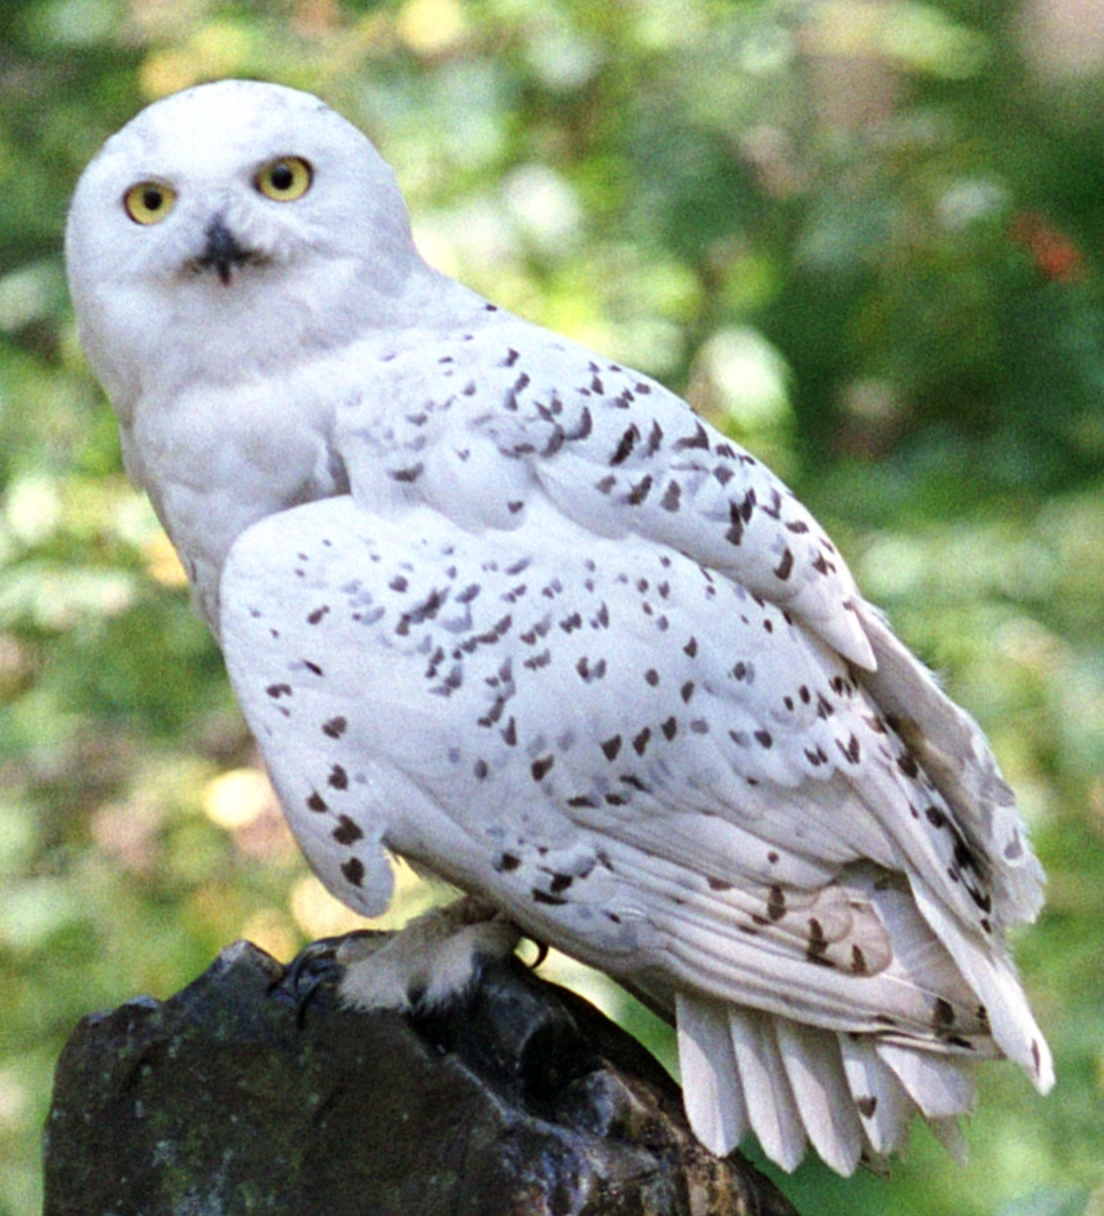
\includegraphics[width=0.25\textwidth]{../shared/images/screenshots/hedwig.jpg}
    };
  \end{tikzpicture}
\end{frame}
  
\begin{frame}{Outline}
  \tableofcontents
  
  \begin{tikzpicture}[remember picture, overlay]
    \node[left] at (current page.east) 
    {
      
\includegraphics[width=0.65\textwidth]{../shared/images/screenshots/outline.jpg}
    };
  \end{tikzpicture}
\end{frame}
  
\section{Introduction}
  
\begin{frame}{Introduction}   
  \textbf{Domestic box office} is the total revenue a movie makes in the United States (+ territories) and Canada. Movie studios report this figure every day, and it is a critical metric for the success of a movie.

  \begin{figure}
    
\includegraphics[width=0.8\textwidth]{../shared/images/screenshots/domesticboxoffice.jpeg}
  \end{figure}
\end{frame}

\begin{frame}{Project Goals}

\begin{itemize}
  \item Model \textbf{daily} domestic box office for every movie in theaters
  \item \textbf{Update model} as new data is available
  \item Use \textbf{no human input} to run
  \item Combine the technical rigor of \textbf{published research} with techniques from \textbf{hobbyists}
\end{itemize}

\begin{figure}
  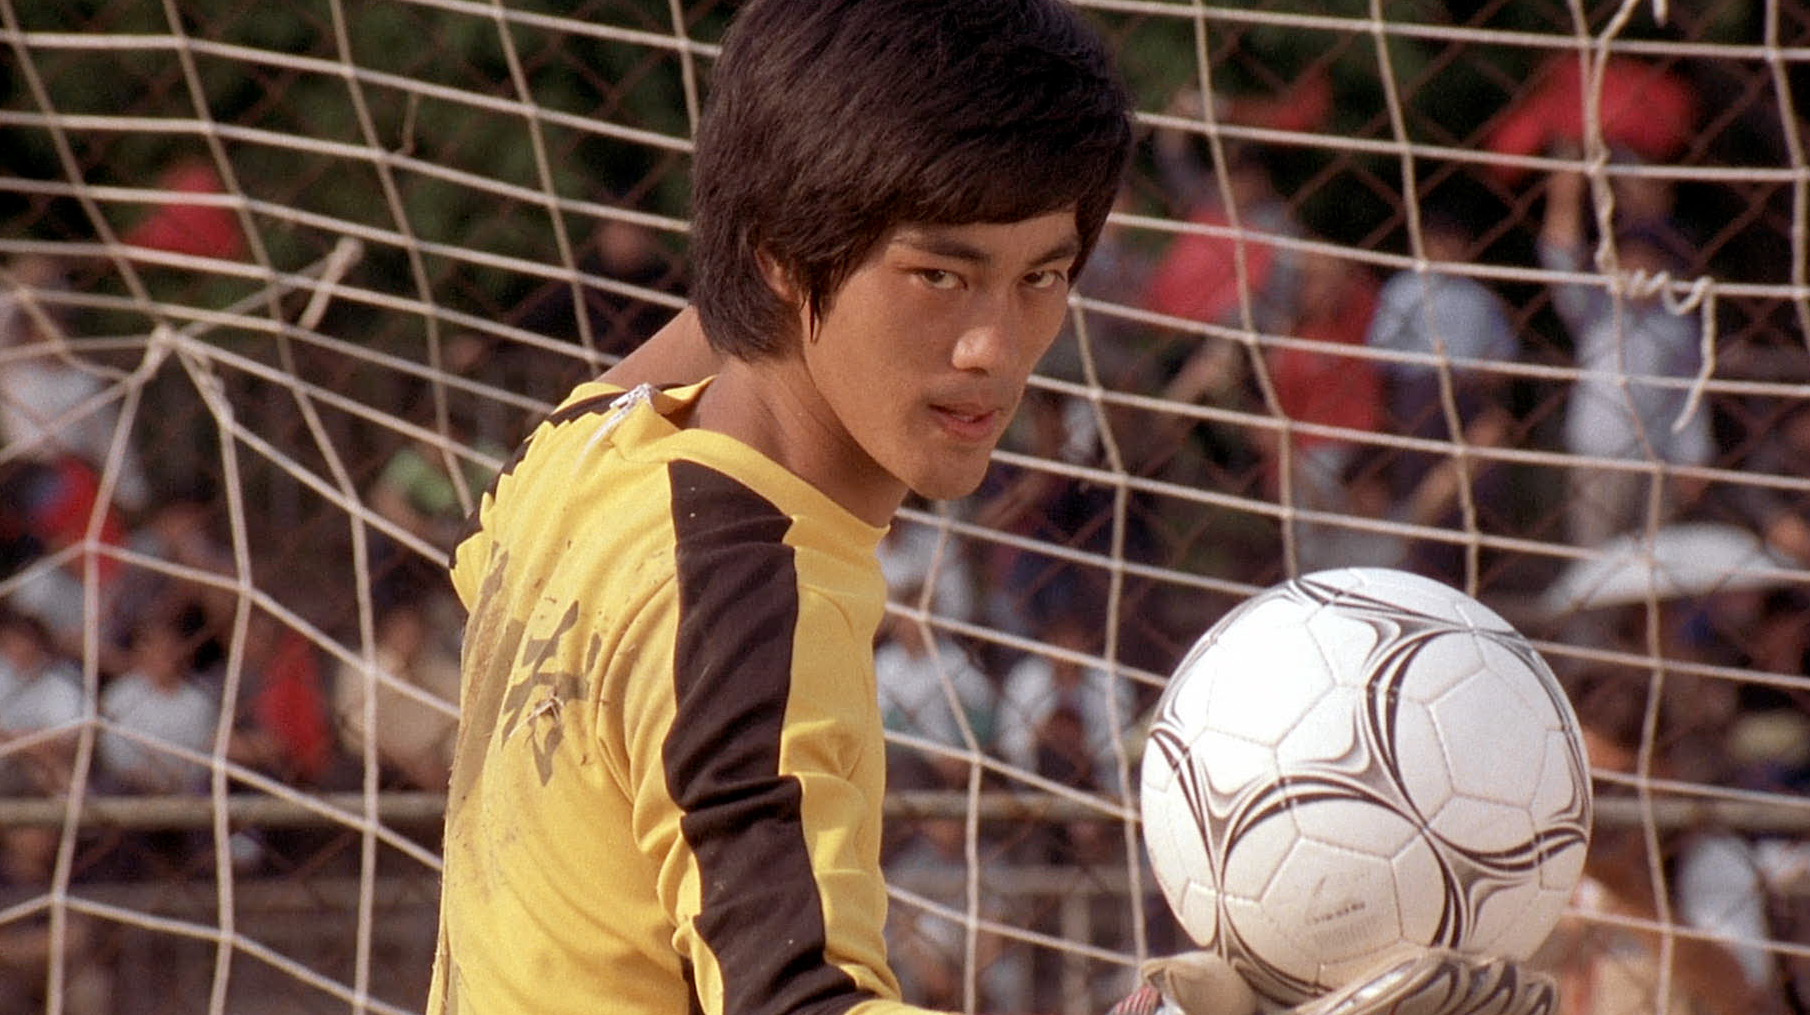
\includegraphics[width=0.6\textwidth]{../shared/images/screenshots/goals.jpg}
\end{figure}
\end{frame}

\begin{frame}{2025 Movies}

% 7 images next to each other
\begin{figure}
  
\includegraphics[width=0.2\textwidth]{../shared/images/posters/avatar3.jpg}
  
\includegraphics[width=0.2\textwidth]{../shared/images/posters/f4.jpg}
  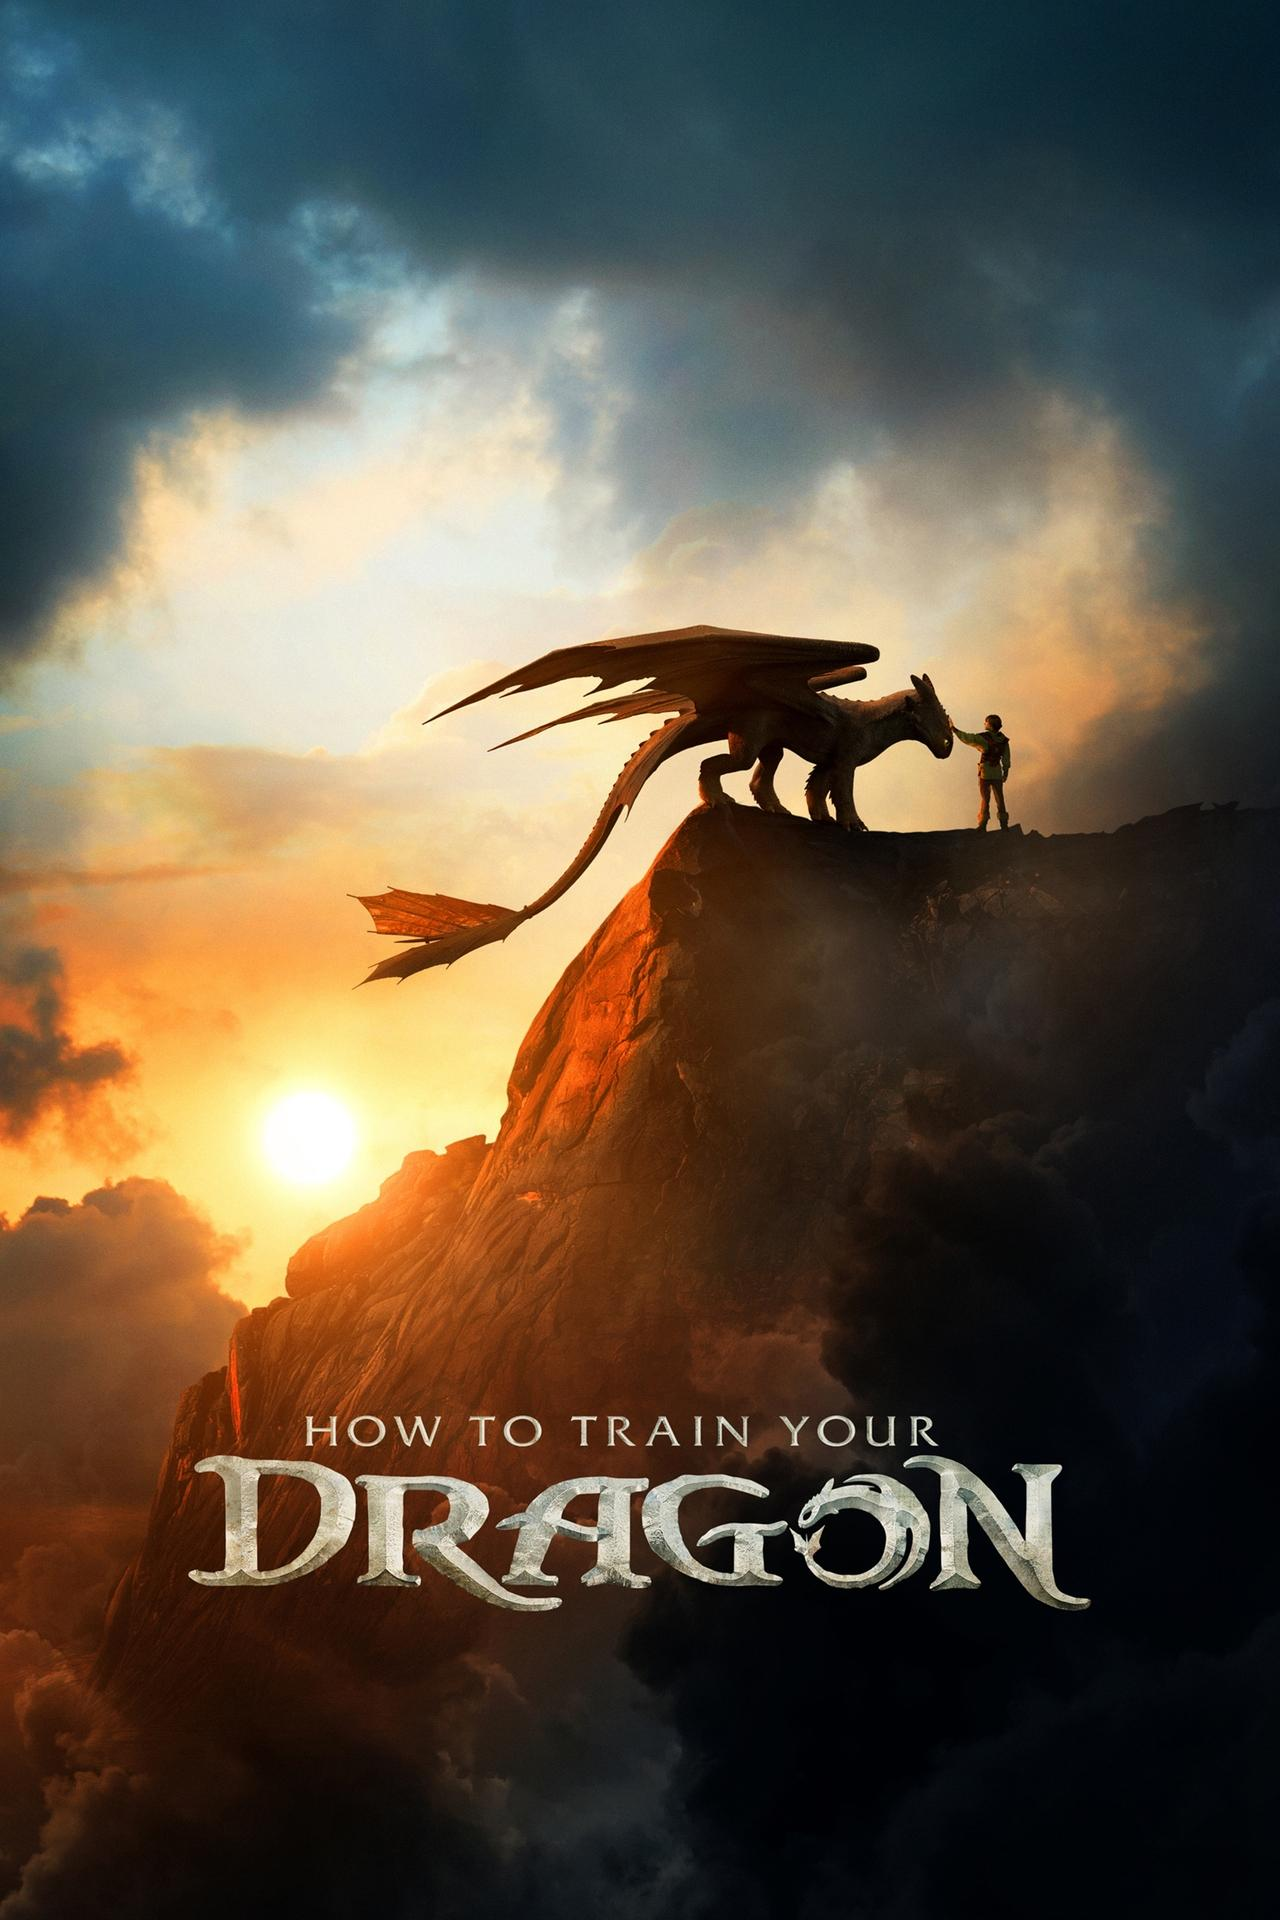
\includegraphics[width=0.2\textwidth]{../shared/images/posters/howtotrainyourdragon.jpg}
  
\includegraphics[width=0.2\textwidth]{../shared/images/posters/jwrebirth.jpg}
  
\includegraphics[width=0.2\textwidth]{../shared/images/posters/minecraft.jpg}
  
\includegraphics[width=0.2\textwidth]{../shared/images/posters/superman.jpg}
  
\includegraphics[width=0.2\textwidth]{../shared/images/posters/wicked2.jpg}
  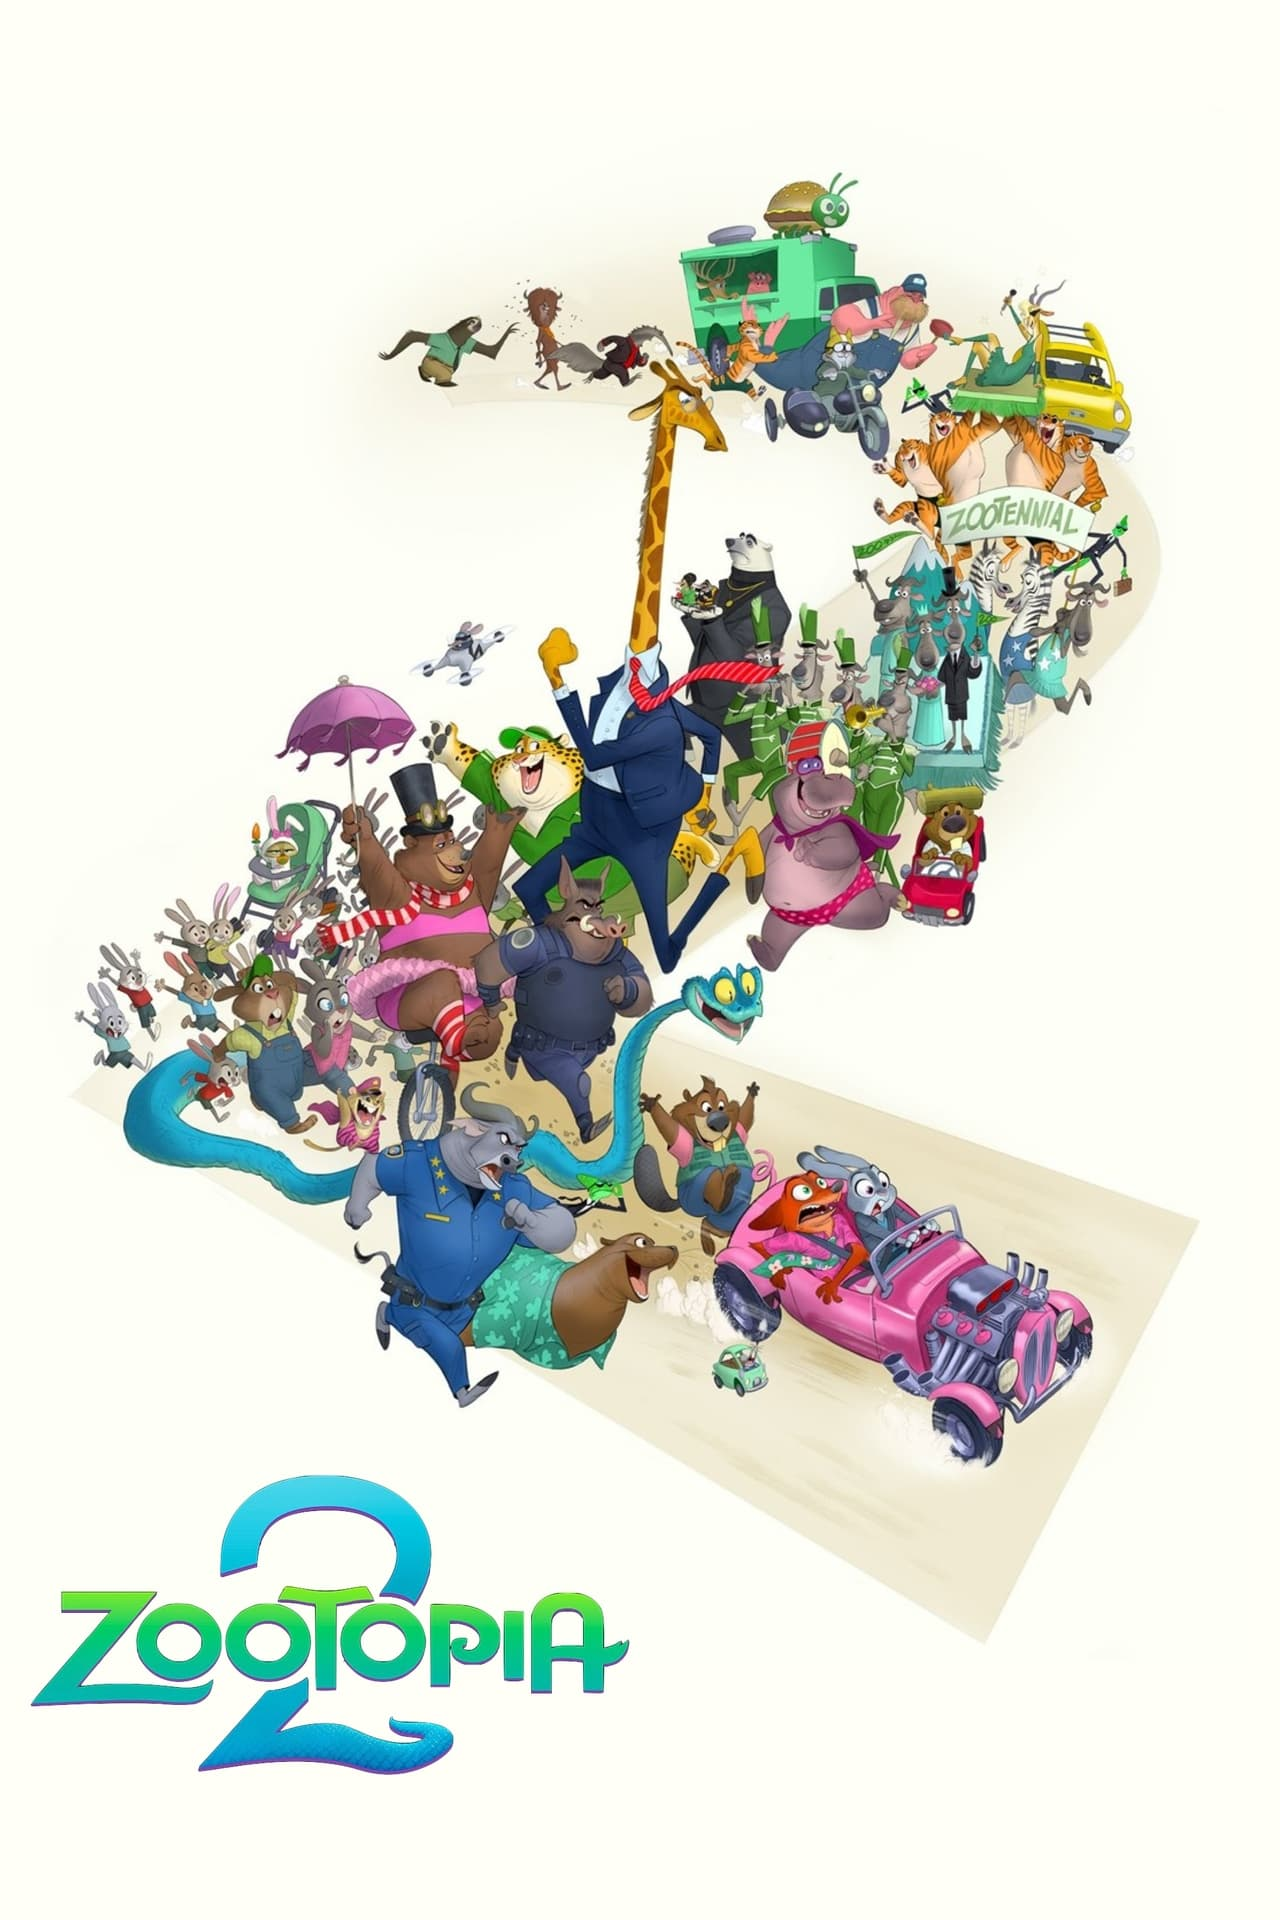
\includegraphics[width=0.2\textwidth]{../shared/images/posters/zootopia2.jpg}
\end{figure}
\end{frame}

\begin{frame}{Yearly Domestic Box Office}

\begin{figure}
  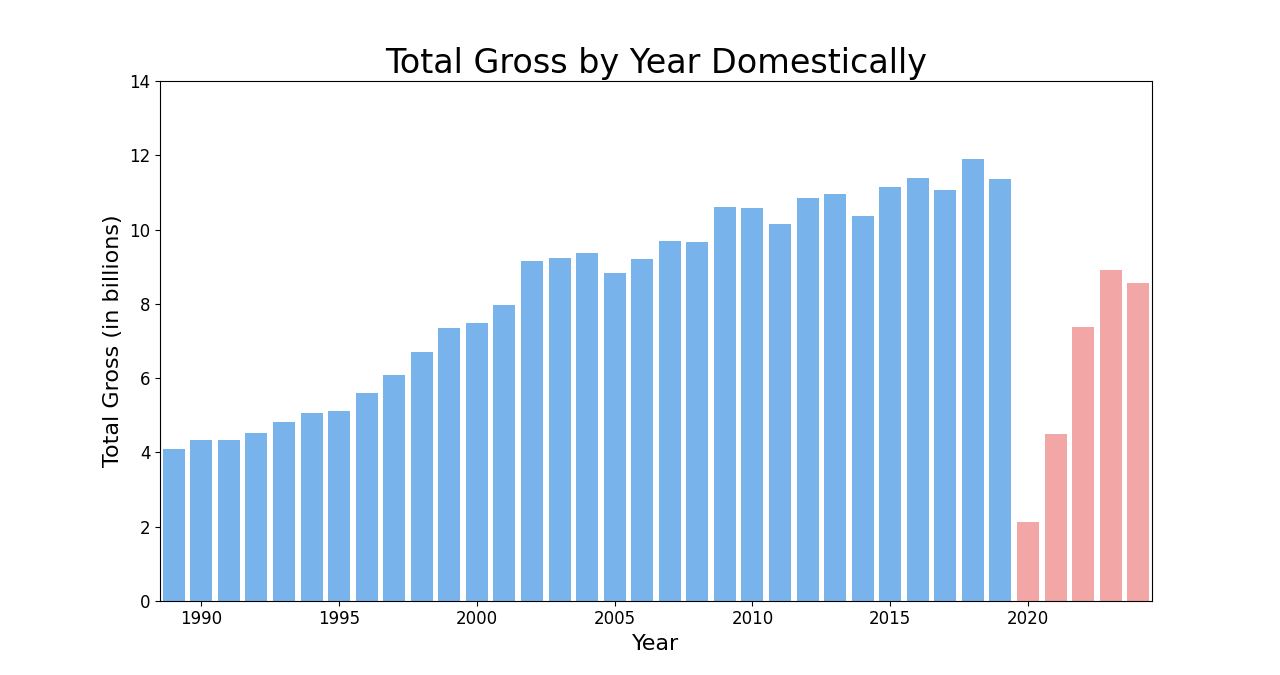
\includegraphics[width=1\textwidth]{../shared/images/yearlygross.png}
\end{figure}
\end{frame}

\begin{frame}{Use Cases}
  \begin{itemize}
    \item Theater Owners
    \item Studios / Distributors
    \item Investors / Executive Producers
    \item Gamblers
    \item Hobbyists
  \end{itemize}
  
  \begin{figure}
    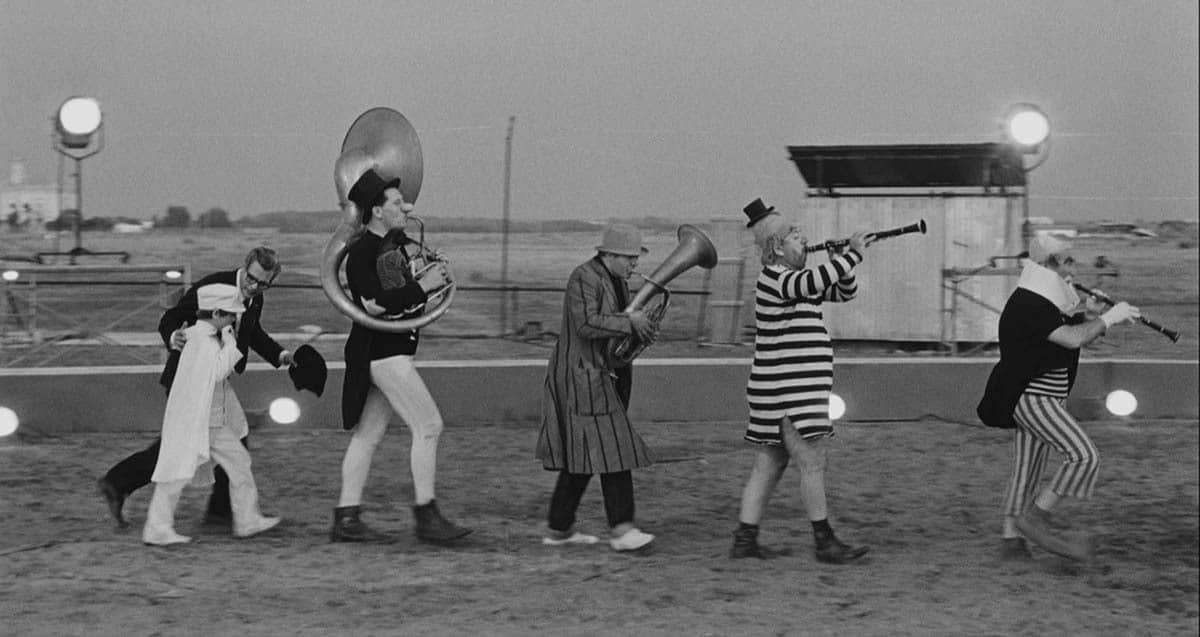
\includegraphics[width=0.6\textwidth]{../shared/images/screenshots/usecases.jpg}
  \end{figure}
\end{frame}

\begin{frame}{Prior Work}
  \textcolor{maroon}{Predicting a full time series from before a movie releases has never been done before in literature}
  \scriptsize
  \begin{itemize}
    \item Previous American works focus on total gross categorization \citep{predictingMovieGrosses,dynamicBayesian,determinantsDomestic}
    \item International works do a limited time series \citep{dailyNeuralNetwork} or classify grosses \citep{boxOfficeInternetData, predictingGrossBoxOffice}
    \item Hobbyists generally focus on weekend predictions \citep{toddMThatcher,boxofficePro,boxofficeReport}
  \end{itemize}
  \normalsize

  \begin{figure}
    
\includegraphics[width=0.6\textwidth]{../shared/images/screenshots/briefcase.jpeg}
  \end{figure}
\end{frame}

\begin{frame}{Release Types}
  % make a table with the release types and then posters
  % wide, limited, IMAX, special engagement, oscar qualifying run, expands wide
  \begin{table}
    \begin{tabular}{cc}
      \textit{Wide (>1000)} & \centered{
\includegraphics[width=0.17\textwidth]{../shared/images/posters/minecraft.jpg}} \\
      \textit{IMAX} & \centered{
\includegraphics[width=0.17\textwidth]{../shared/images/posters/mickey17.jpg}}\\
    \end{tabular}
    \hfill
    \begin{tabular}{rl}
      \textit{Limited (<1000)} & \centered{
\includegraphics[width=0.17\textwidth]{../shared/images/posters/penguinlessons.jpg}} \\
      \textit{Expands Wide} & \centered{
\includegraphics[width=0.17\textwidth]{../shared/images/posters/brutalist.jpg}} \\
    \end{tabular}
  \end{table}

  Other types include \textit{Oscar Qualifying Run} and \textit{Special Engagement}
\end{frame}

\section{Data}

\begin{frame}{Data Gathering}

\begin{itemize}
  \item \textbf{\cite{numbersHome}}: revenue, theater counts, MPAA rating
  \item \textbf{\cite{tmdbHome}}: budget, production company, production country, spoken languages, genres, TMDB rating
  \item \textbf{\cite{imdbHome}}: IMDb rating, metacritic score
  \item \textbf{\cite{pipedGithub}}: YouTube trailers views
  \item \textbf{\cite{wikipediaPageViews}}: Wikipedia page views
\end{itemize}

\begin{figure}
  
\includegraphics[width=0.6\textwidth]{../shared/images/screenshots/datagathering.jpg}
\end{figure}
\end{frame}

\begin{frame}{Data Size}
\begin{itemize}
  \item \textbf{2,940 movies} (all in theaters and on TMDB since 2015)
  \item 137,000 box office days
  \item 124,000 cast and crew records
  \item 355 collections (franchises)
  \item 240,000 movie info days
  \item 80,000 people
  \item 4,585 production companies
  \item 85 spoken languages
\end{itemize}

\begin{tikzpicture}[remember picture, overlay]
  \node[above left] at (current page.south east) 
  {
      
\includegraphics[width=0.53\textwidth]{../shared/images/screenshots/biggerboat.jpg}
  };
\end{tikzpicture}
\end{frame}

\section{Modeling}

\begin{frame}{The Gerber Method}
  % general process of multipliers
  \begin{enumerate}
    \item Find \textbf{comparison (comp)} movies to the target movie
    \item Calculate \textbf{seasonal multipliers}
    \item Calculate \textbf{weekly multipliers} using comps
    \item Calculate \textbf{daily multipliers} using comps
    \item Apply the values!
  \end{enumerate}

  \begin{figure}
    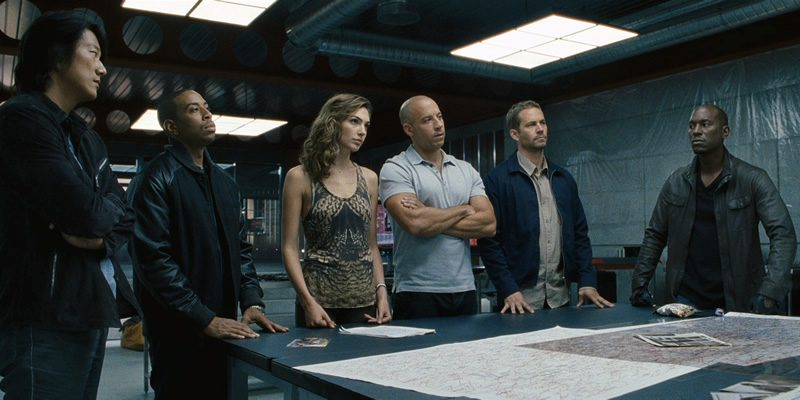
\includegraphics[width=0.7\textwidth]{../shared/images/screenshots/heistplanning.jpg}
  \end{figure}
\end{frame}

\begin{frame}{Step 1: Finding Comps}
  Given weights $w_i$ where $i$ is each of the 12 features, the distance $d$ between two movies is given by:
  \begin{equation*}
    d = \sum_{i=1}^{12} w_i \cdot (x_i - y_i)
  \end{equation*}
  where $x_i$ and $y_i$ are the values of the features for the two movies. 
  \\
  The comps are the \textbf{8} movies with the smallest distance to the target movie. 
  \\
  Weights are found using randomized grid search.
  \begin{figure}
    
\includegraphics[width=0.45\textwidth]{../shared/images/screenshots/whataboutmath.jpg}
  \end{figure}
\end{frame}

\begin{frame}{KNN Features}
  Features of interest:
  \begin{itemize}
    \item Budget
    \item Genres
    \item MPAA Rating
    \item Production companies
    \item Production countries
    \item Production method
    \item Release types
    \item Screenplay source
    \item Spoken languages
  \end{itemize}

  % explain how to find comparisons movies to generate the multipliers
  \begin{tikzpicture}[remember picture, overlay]
    \node[left] at (current page.east) 
    {
        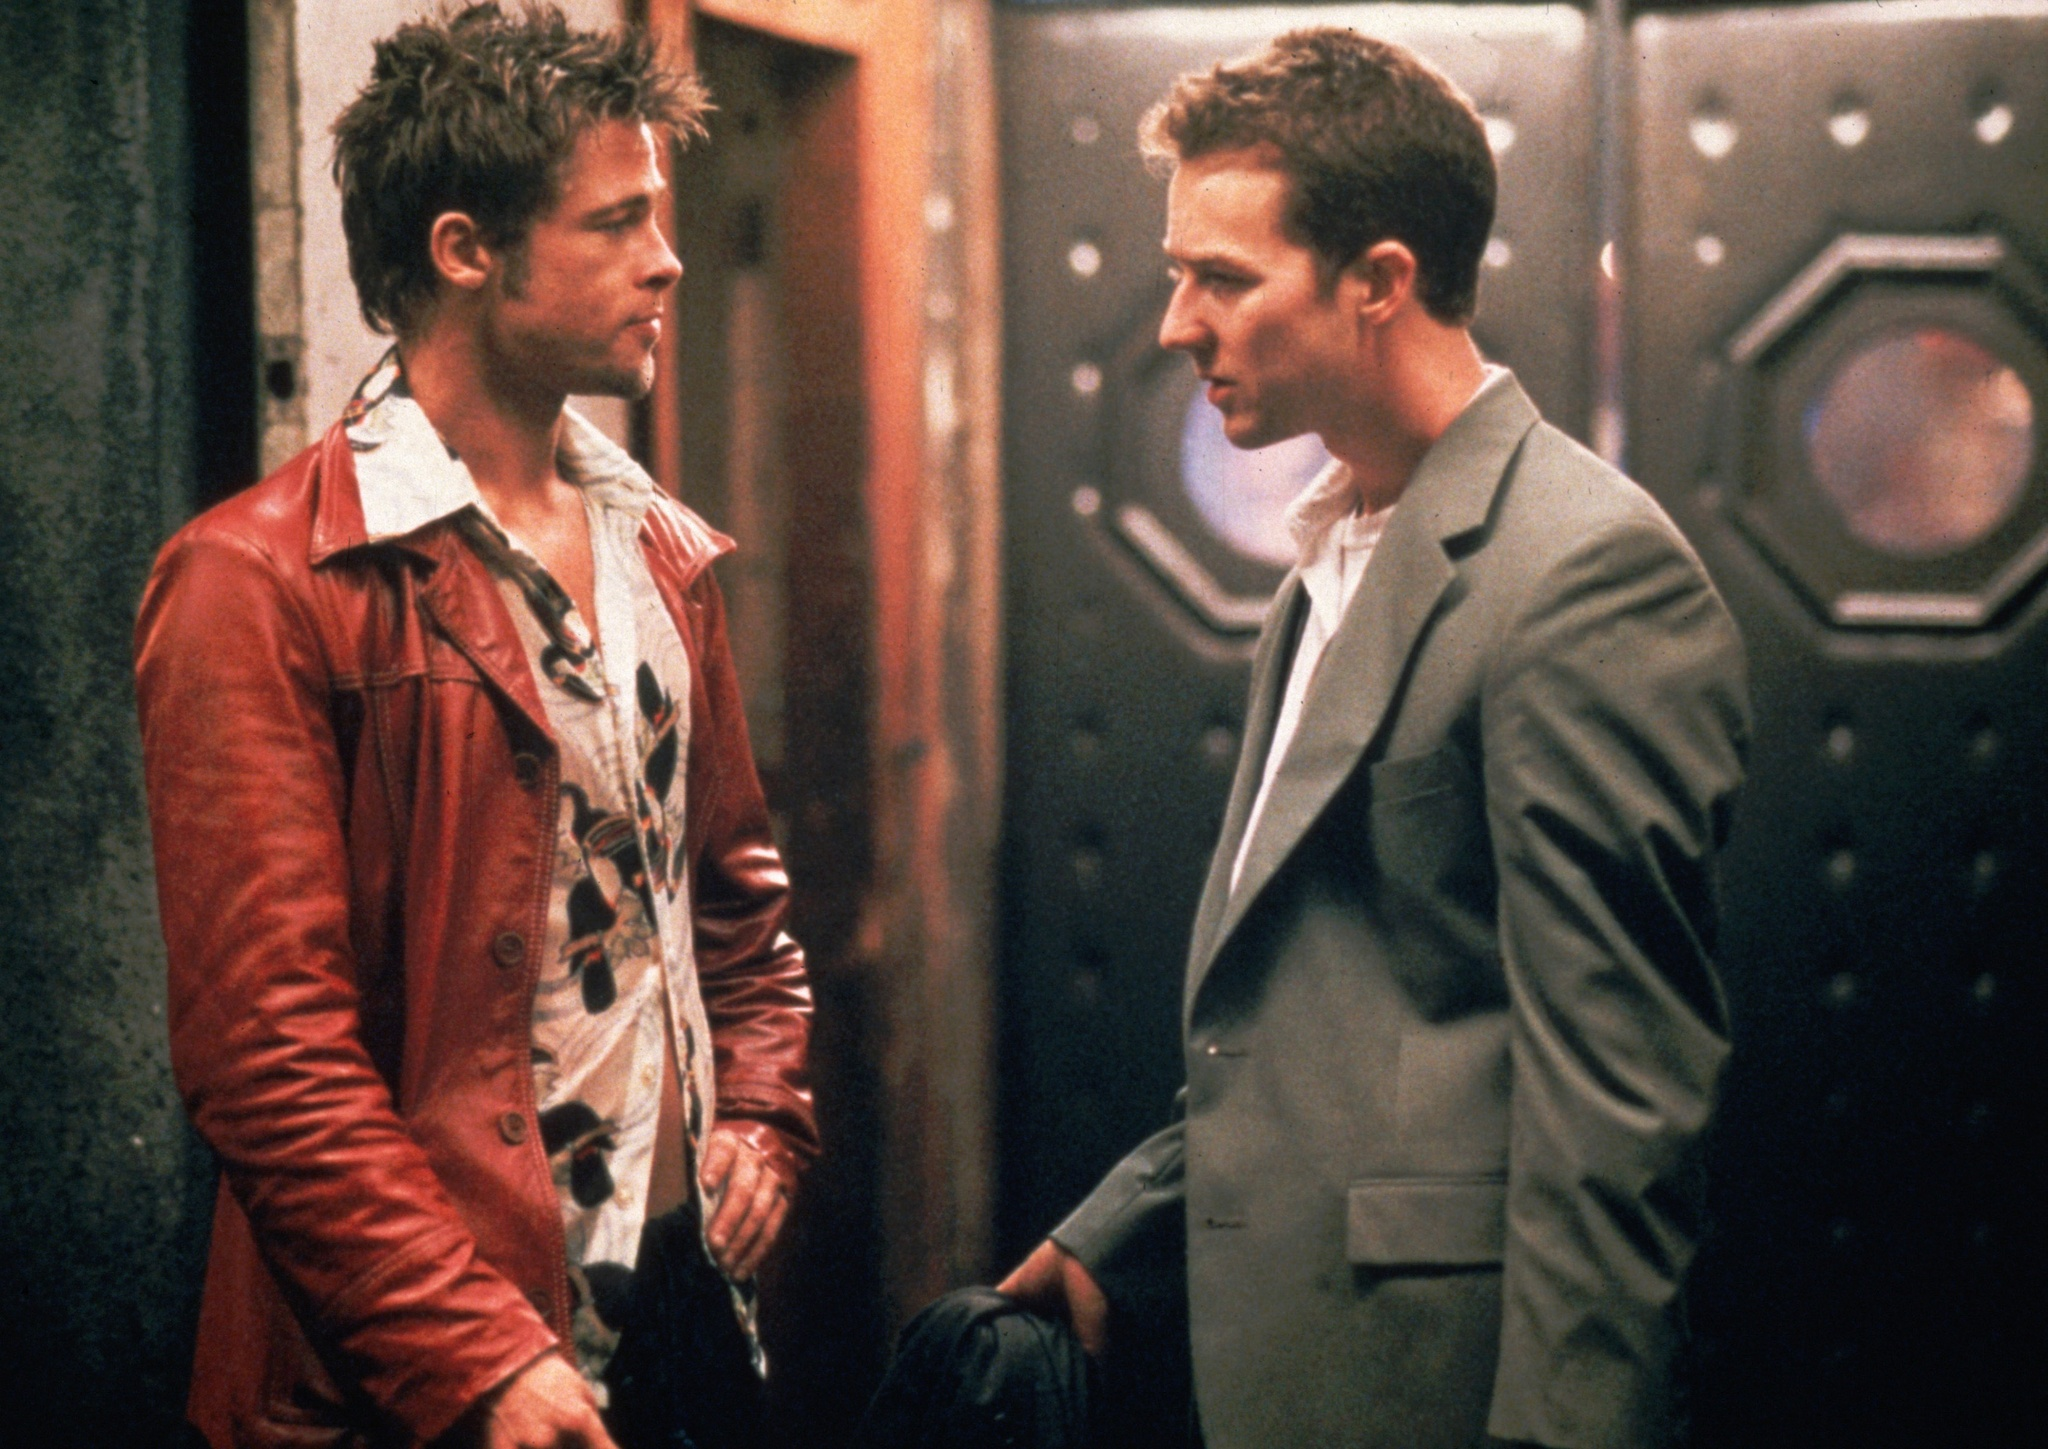
\includegraphics[width=0.6\textwidth]{../shared/images/screenshots/comparing.jpg}
    };
  \end{tikzpicture}
\end{frame}

\begin{frame}{Example: \cite{conclave} Comps}
  \begin{figure}
    \begin{minipage}{0.27\textwidth}
      
\includegraphics[width=\textwidth]{../shared/images/posters/conclave.jpg}
    \end{minipage}
    \hfill
    \begin{minipage}{0.71\textwidth}
      
\includegraphics[width=0.242\textwidth]{../shared/images/posters/hauntinginvenice.jpg}
      
\includegraphics[width=0.242\textwidth]{../shared/images/posters/girlonthetrain.jpg}
      
\includegraphics[width=0.242\textwidth]{../shared/images/posters/artofracingintherain.jpg}
      
\includegraphics[width=0.242\textwidth]{../shared/images/posters/americanassassin.jpg}
      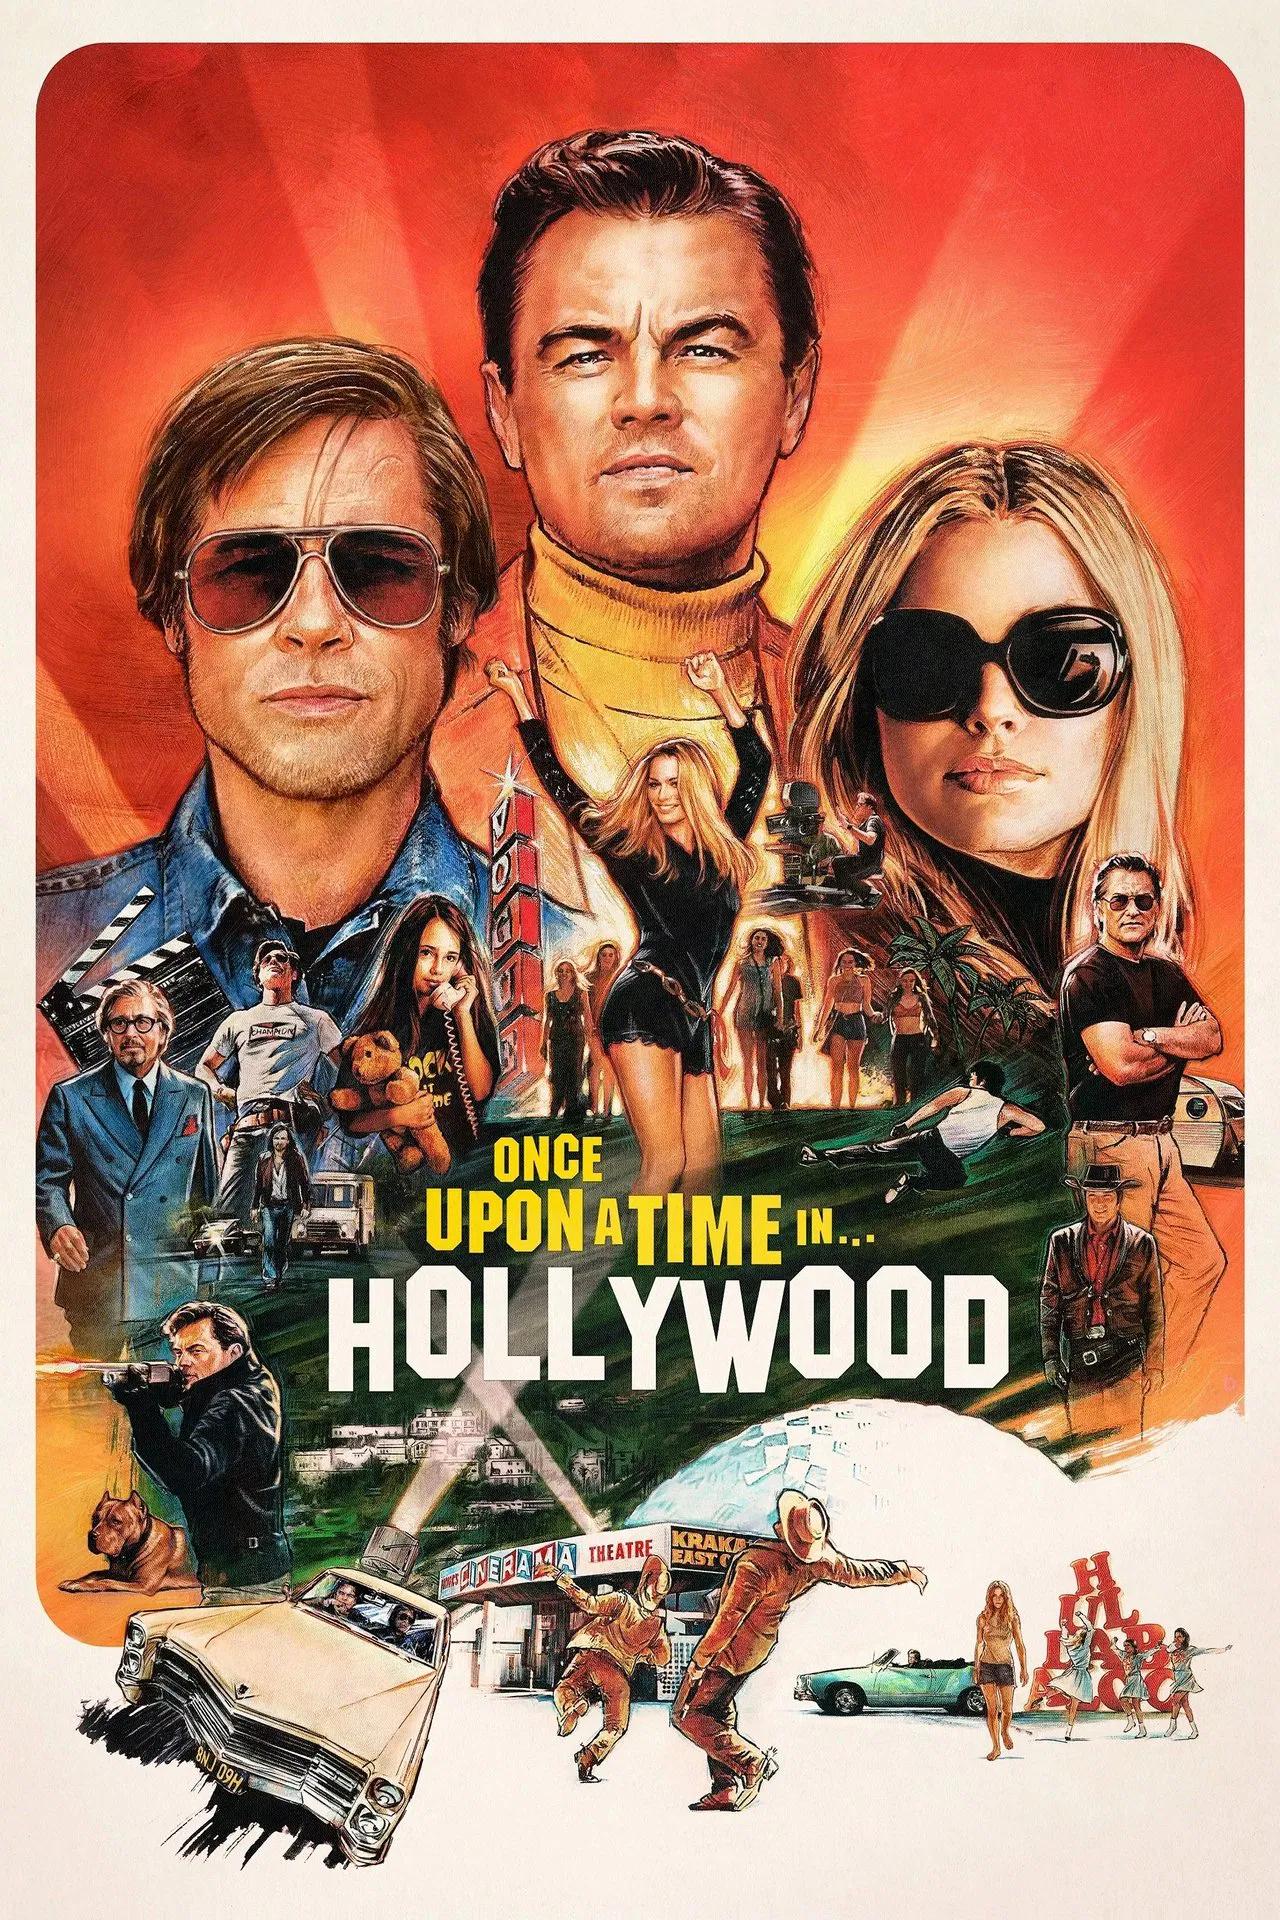
\includegraphics[width=0.242\textwidth]{../shared/images/posters/onceuponatime.jpg}
      
\includegraphics[width=0.242\textwidth]{../shared/images/posters/notimetodie.jpg}
      
\includegraphics[width=0.242\textwidth]{../shared/images/posters/missing.jpg}
      
\includegraphics[width=0.242\textwidth]{../shared/images/posters/therhythmsection.jpg}
    \end{minipage}
  \end{figure}
\end{frame}

\begin{frame}{\cite{conclave} Comps Multipliers}
  \begin{figure}
    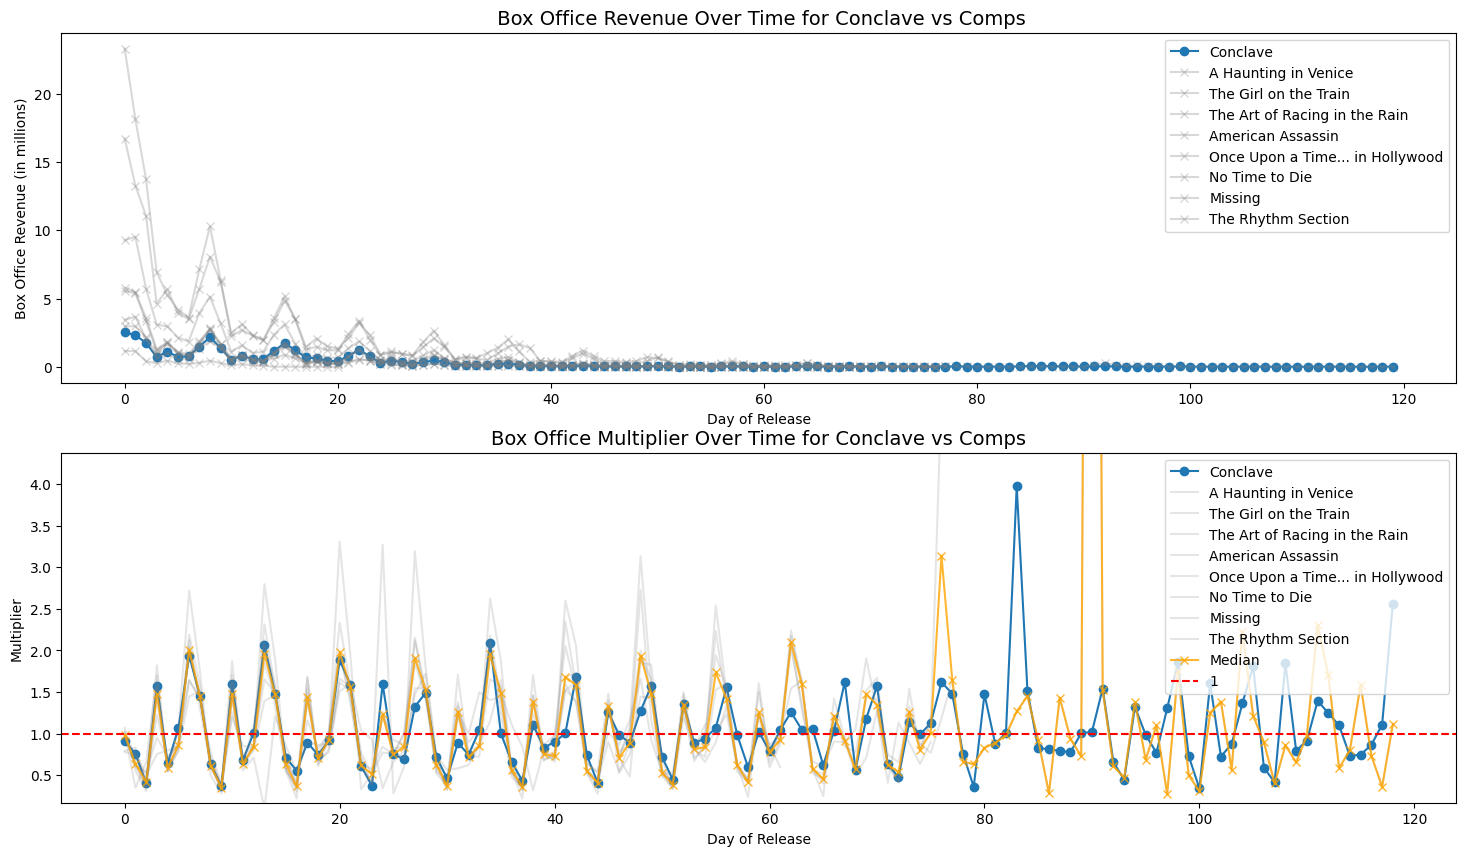
\includegraphics[width=0.95\textwidth]{../shared/images/conclavecomps.png}
  \end{figure}
\end{frame}

\begin{frame}{Zoomed \cite{conclave} Comps Multipliers}
  \begin{figure}
    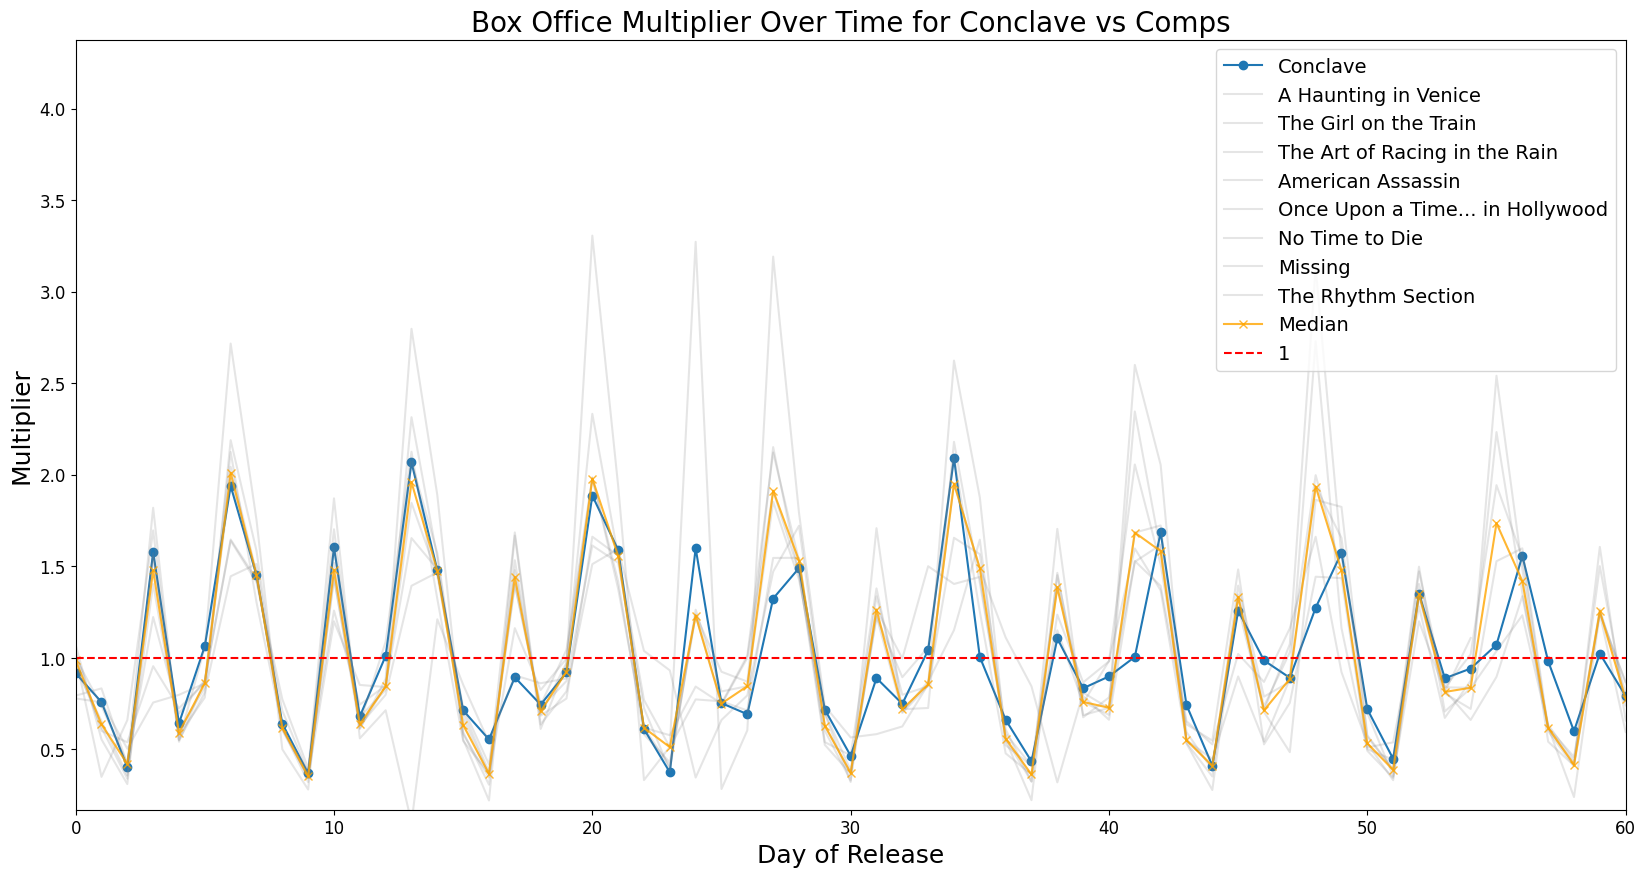
\includegraphics[width=1\textwidth]{../shared/images/conclavecompszoom.png}
  \end{figure}

  \addtocounter{framenumber}{-1}
\end{frame}

\begin{frame}{Step 2: Seasonal Multipliers}
  \begin{itemize}
    \item Movies make more money during summer and winter seasons
    \item Movies also make more money on certain holidays
    \item To compare movies, we need to \textbf{adjust} for these factors
  \end{itemize}

  \begin{figure}
    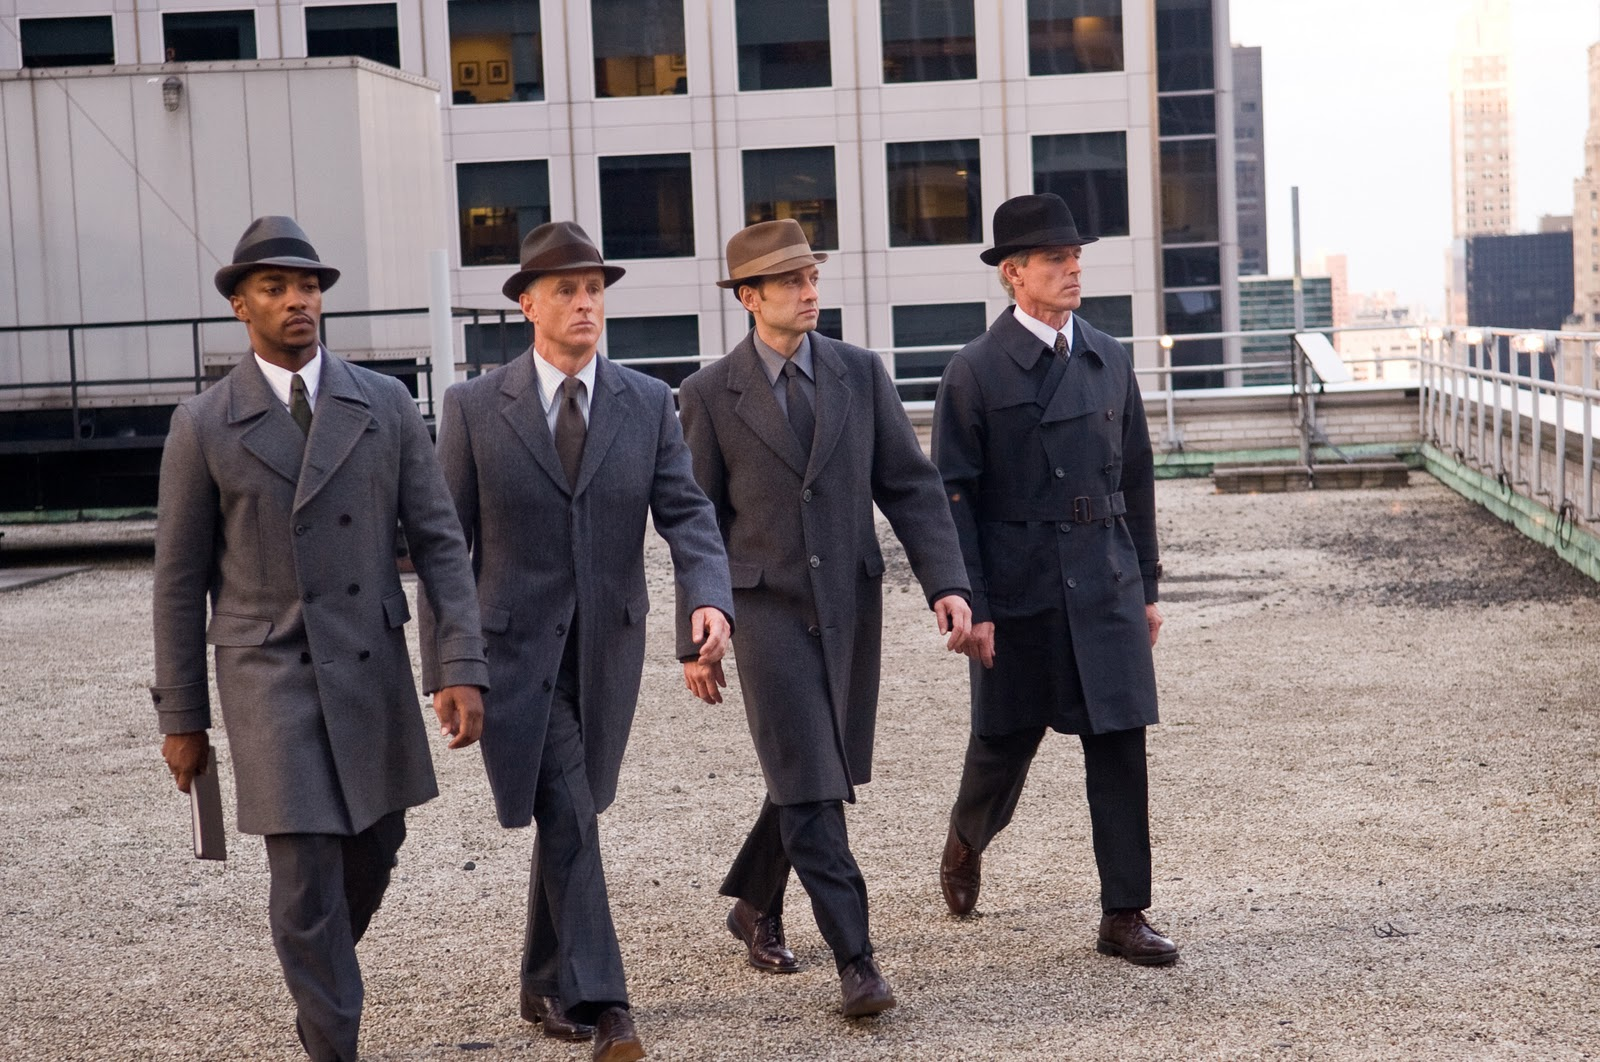
\includegraphics[width=0.65\textwidth]{../shared/images/screenshots/adjustment.jpg}
  \end{figure}
\end{frame}

\begin{frame}{How Much They Make}
  \begin{figure}
    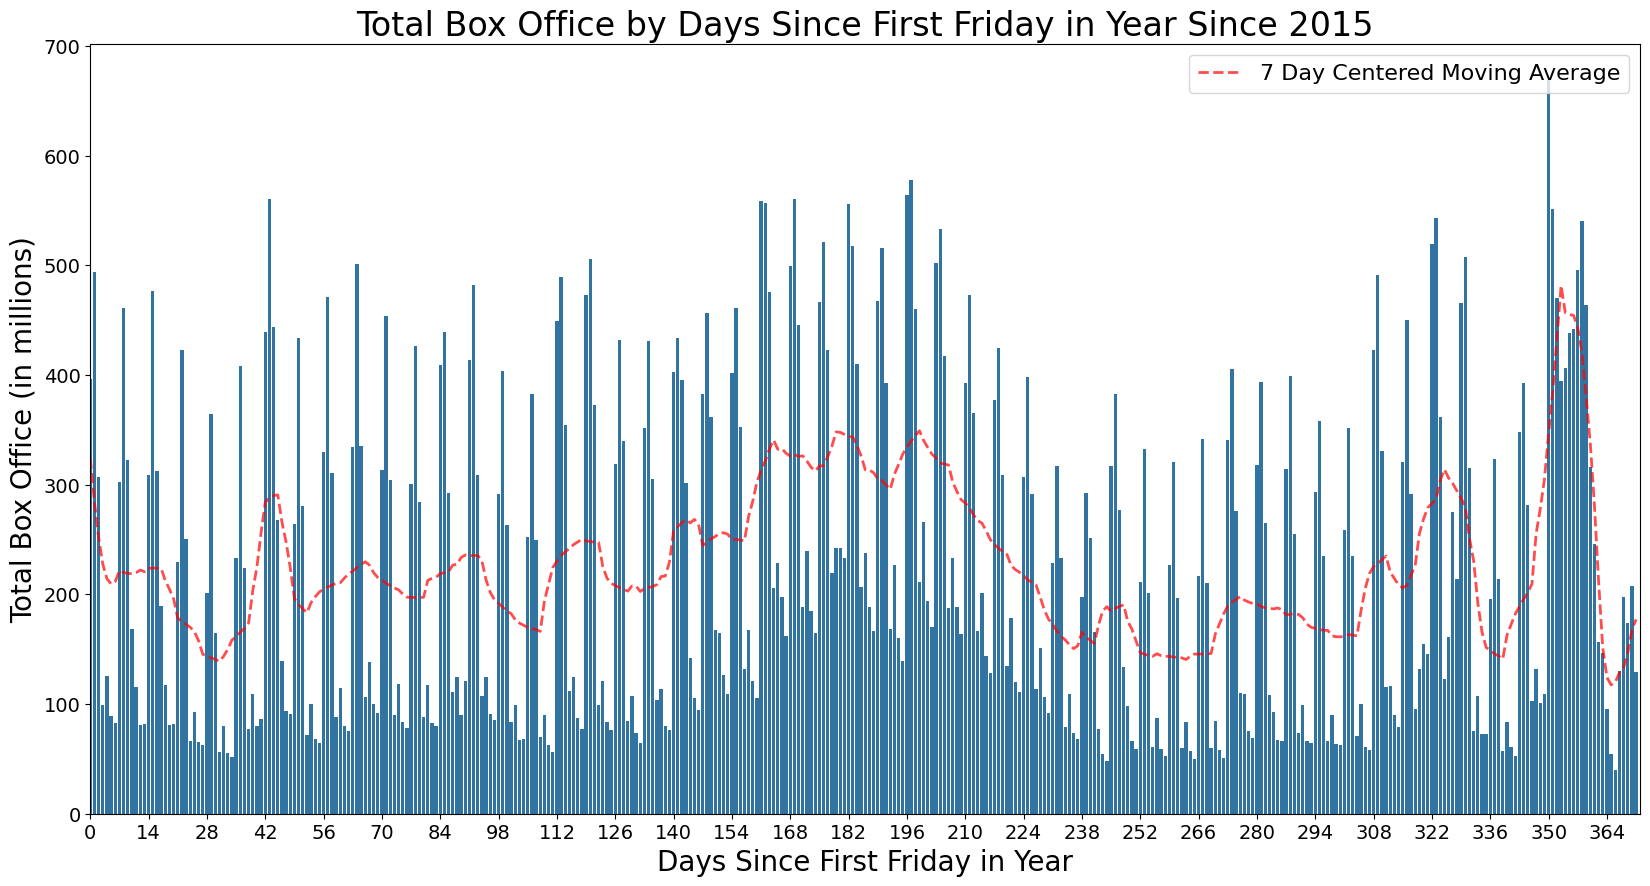
\includegraphics[width=1.0\textwidth]{../shared/images/boxoffice.png}
  \end{figure}
\end{frame}

\begin{frame}{How Much They Cost}
  \begin{figure}
    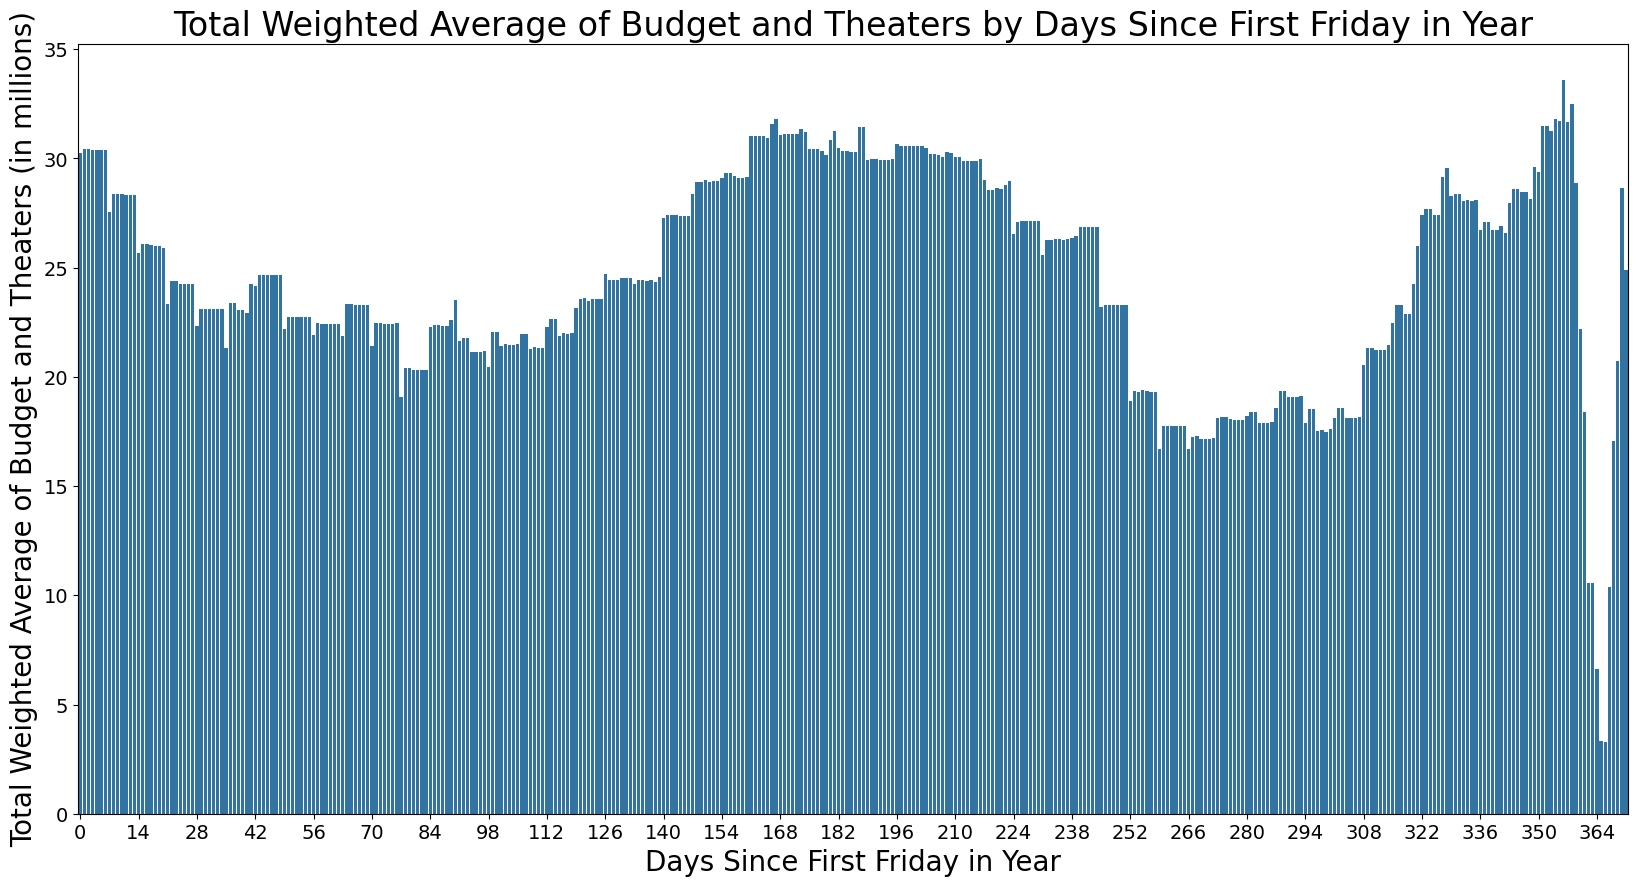
\includegraphics[width=1.0\textwidth]{../shared/images/weighteddays.png}
  \end{figure}
\end{frame}

\begin{frame}{Seasonal Multipliers}
  \begin{figure}
    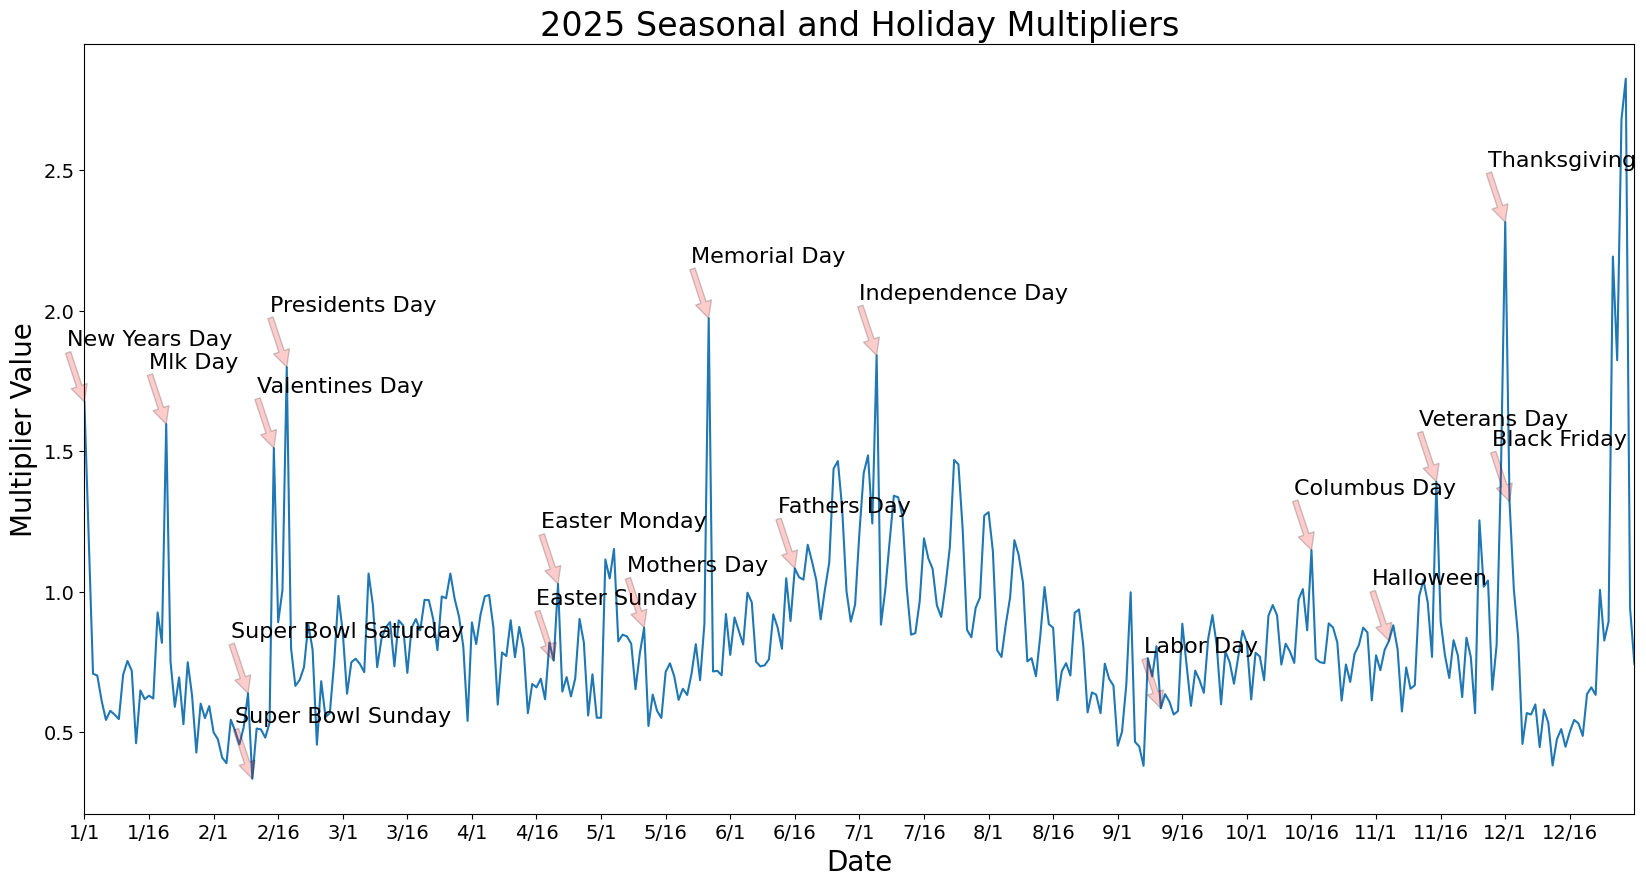
\includegraphics[width=1.0\textwidth]{../shared/images/adjustments.png}
  \end{figure}
\end{frame}

\begin{frame}{Step 3: Weekly Multipliers}
  \begin{itemize}
    \item Movie grosses decrease each week in a generally exponential pattern
    \item Take the median of weekly \textit{drops} for each comparison movie as it changes by week
    \item If the target movie has been out for more than 7 days, consider its own past drops as well
  \end{itemize}

  \begin{figure}
    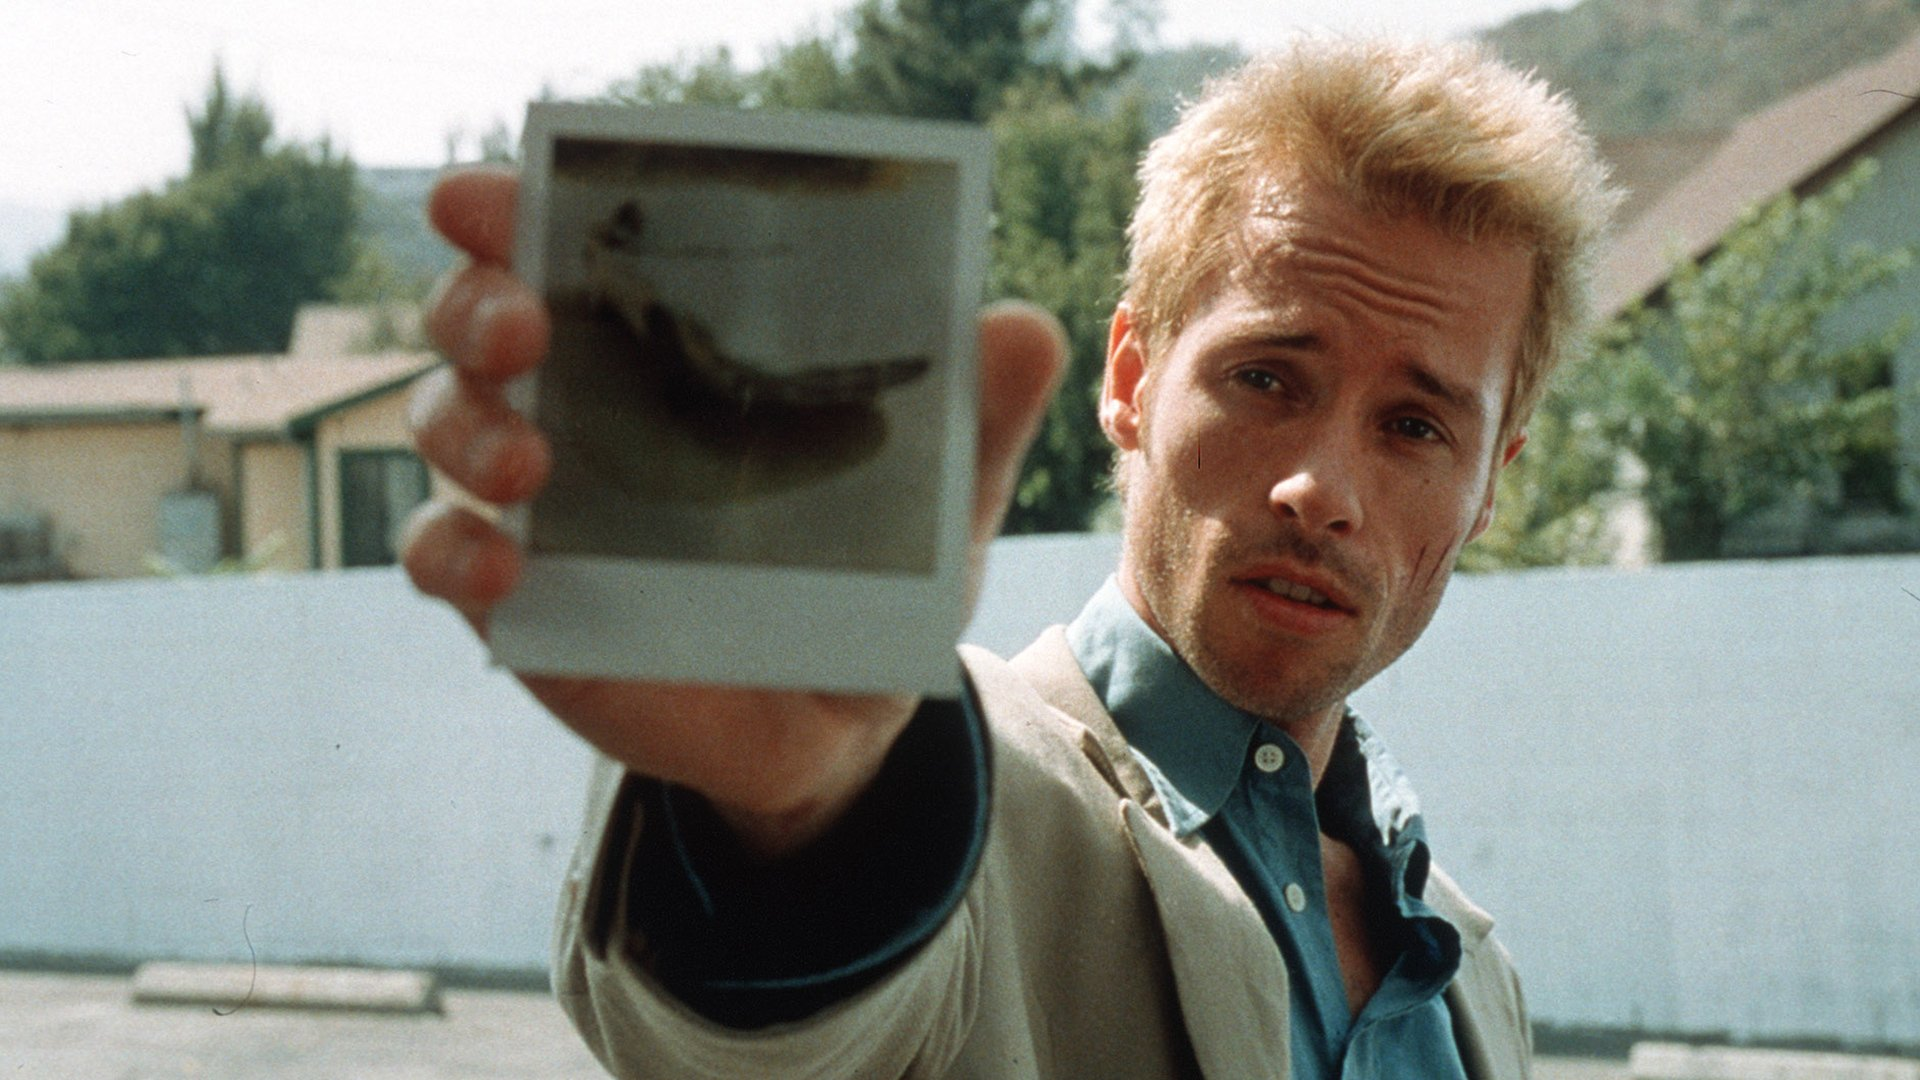
\includegraphics[width=0.55\textwidth]{../shared/images/screenshots/drops.jpg}
  \end{figure}
\end{frame}

\begin{frame}{Why Weekly Multipliers}
  \begin{figure}
    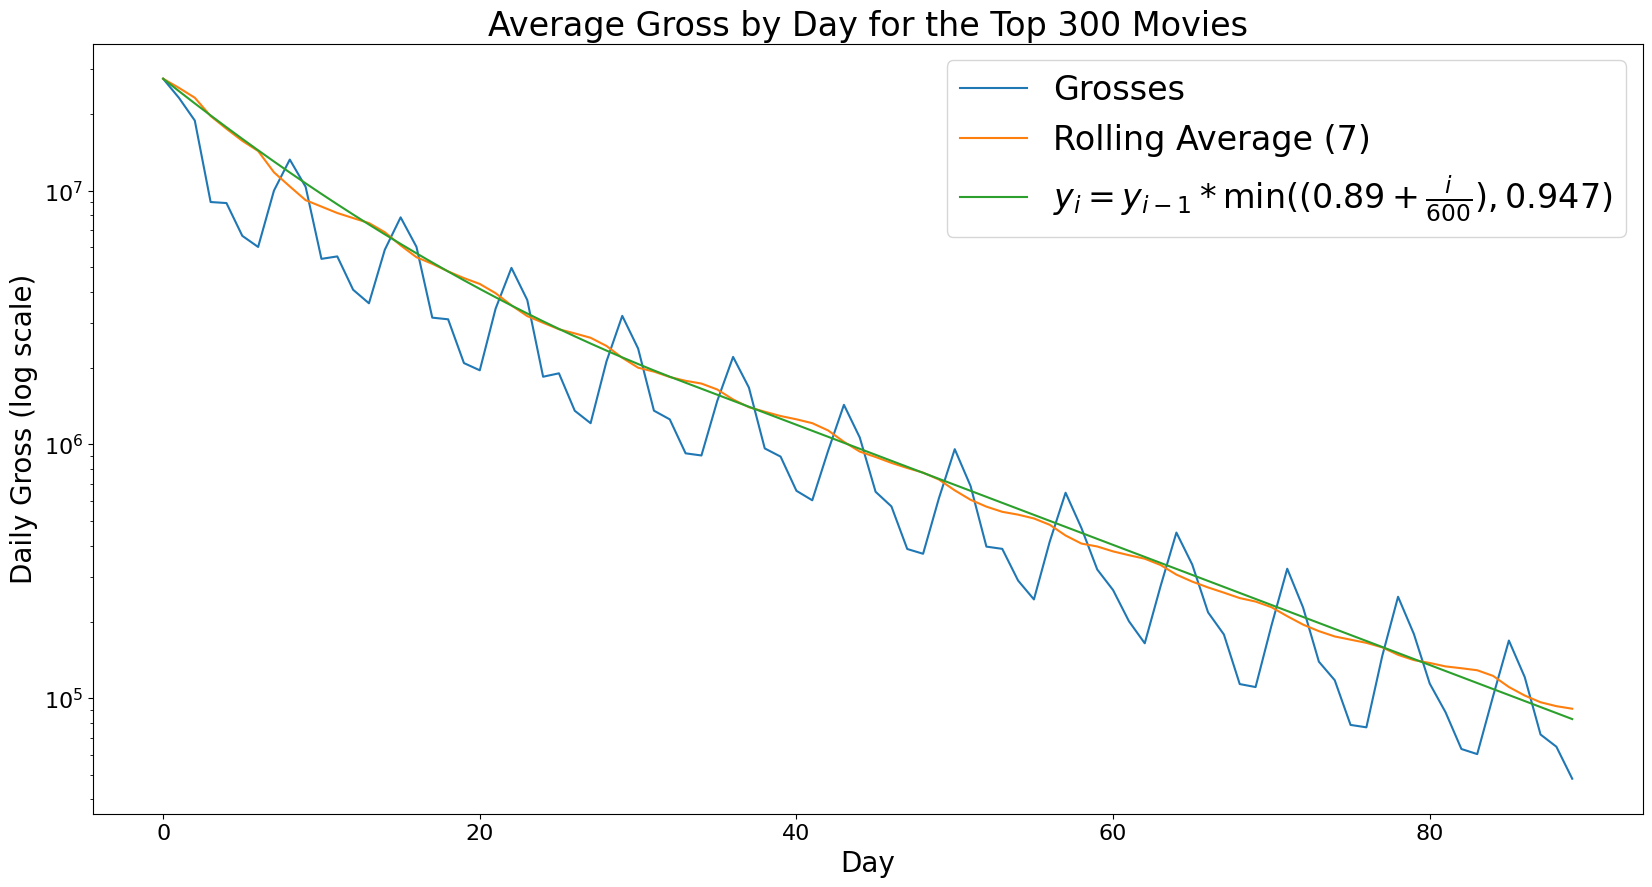
\includegraphics[width=1.0\textwidth]{../shared/images/top300fancy.png}
  \end{figure}
\end{frame}

\begin{frame}{Step 4: Daily Multipliers}
  \begin{itemize}
    \item Movies make more money on weekends than weekdays
    \item The pattern of multipliers is different for each day of the week but is generally consistent between weeks
    \item Take the weighted average of the daily changes for each comparison movie
    \item Use that weighted average to create 7 values, one for each day of the week
  \end{itemize}

  \begin{figure}
    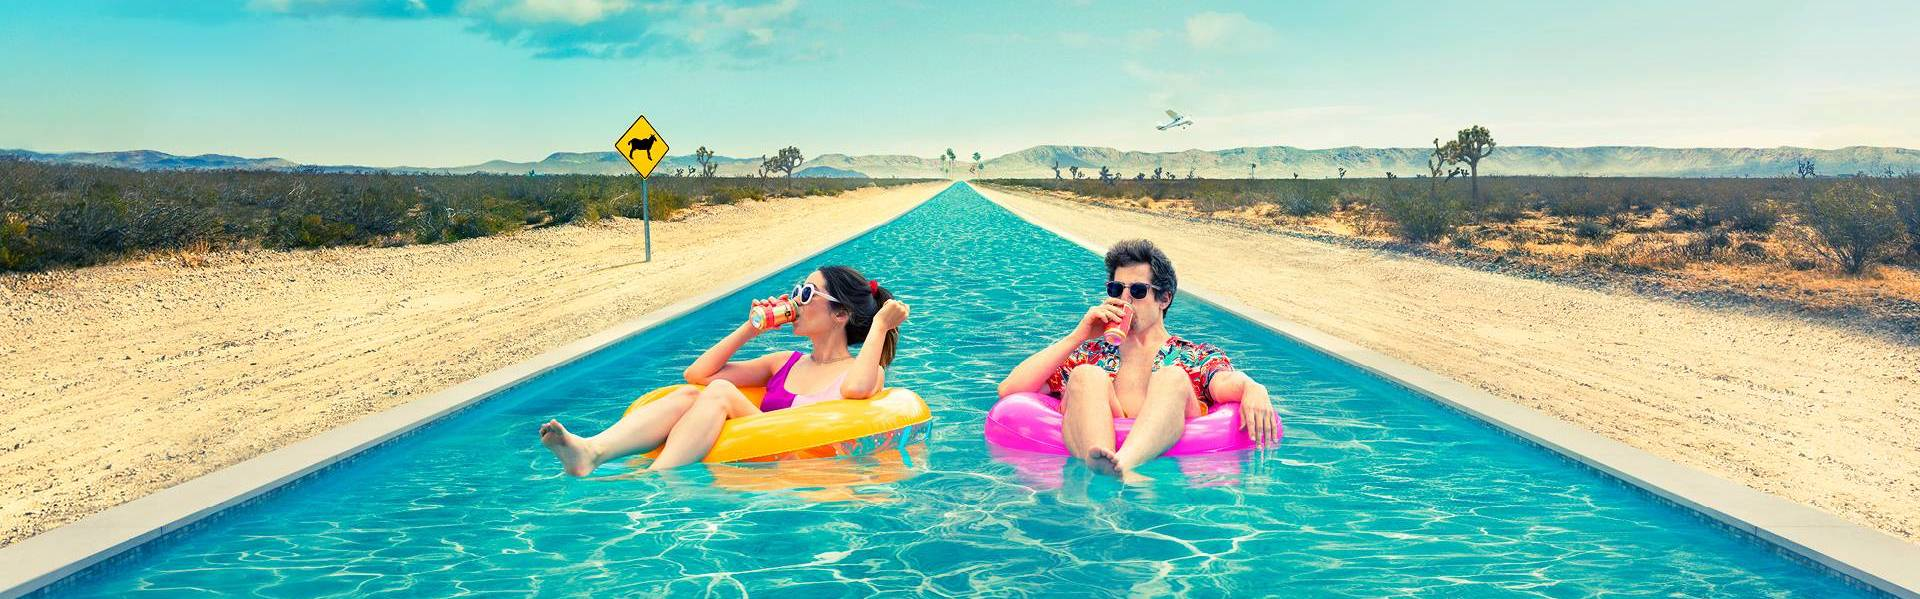
\includegraphics[width=0.65\textwidth]{../shared/images/screenshots/mult.jpg}
  \end{figure}
\end{frame}

\begin{frame}{Median Daily Multipliers}
  % explain how to find multipliers for the target movie
  \begin{table}
    \begin{tabular}{cc}
      \hline
      \textbf{Days} & \textbf{Median Multiplier} \\ \hline
      Monday -> Tuesday & 1.28 \\
      Tuesday -> Wednesday & 0.75 \\
      Wednesday -> Thursday & 0.92 \\
      Thursday -> Friday & 2.86 \\
      Friday -> Saturday & 1.60 \\
      Saturday -> Sunday & 0.66 \\
      Sunday -> Monday & 0.35 \\ \hline
    \end{tabular}
  \end{table}

  \begin{figure}
    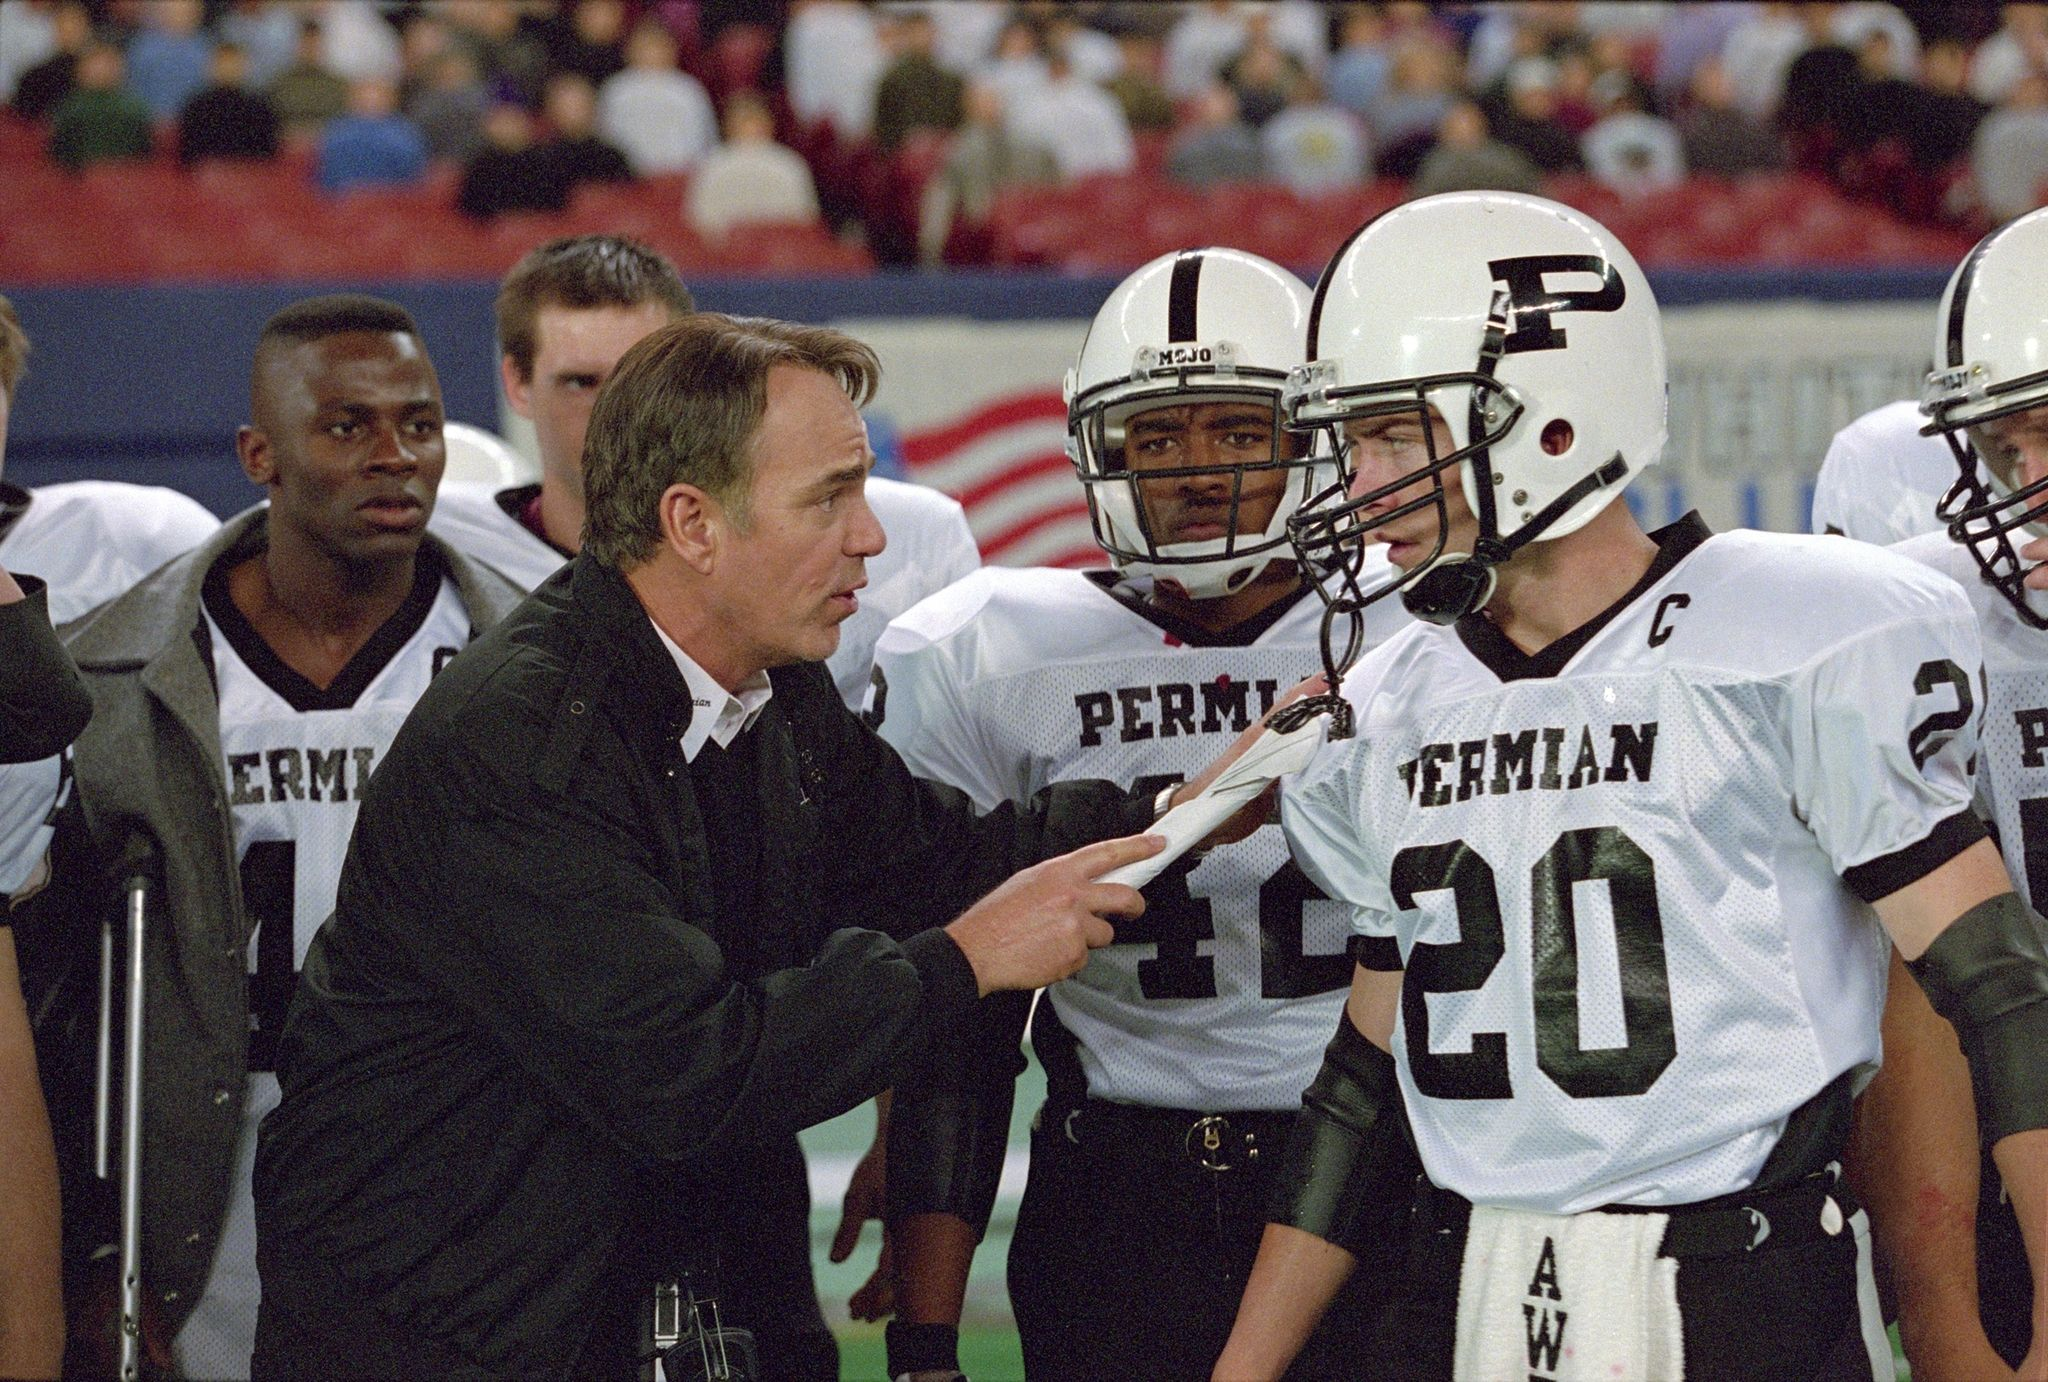
\includegraphics[width=0.35\textwidth]{../shared/images/screenshots/fridaynightlights.jpg}
  \end{figure}
\end{frame}

\begin{frame}{Step 5: Apply the Values}
\begin{equation*}
  \text{rev}_{n+1} = \text{rev}_{n} \times \text{weekly}_{\lfloor n/7 \rfloor}^{1/7} \times \text{daily}_{n \bmod 7} \times \frac{\text{seasonal}_{date_{n+1}}}{\text{seasonal}_{date_n}}
\end{equation*}
where:
\begin{align*}
    \text{rev}_{n} &= \text{revenue on day n} \\
    \text{seasonal} &= \text{seasonal mult for the day of the year} \\
    \text{weekly} &= \text{array of max comp length} \\
    \text{daily} &= \text{array of length 7 with daily mults for each day of the week}
\end{align*}

\begin{figure}
  
\includegraphics[width=0.3\textwidth]{../shared/images/screenshots/aladdin.jpg}
\end{figure}
\end{frame}

\section{Results}

\begin{frame}
  % 3 images
  \begin{figure}
    
\includegraphics[width=0.2\textwidth]{../shared/images/posters/twisters.jpg}
    
\includegraphics[width=0.2\textwidth]{../shared/images/posters/monkeyman.jpg}
    
\includegraphics[width=0.2\textwidth]{../shared/images/posters/meangirls.jpg}
  \end{figure}

  \begin{center}
    \textbf{Results}
  \end{center}

  \begin{figure}
    
\includegraphics[width=0.2\textwidth]{../shared/images/posters/joker2.jpg}
    
\includegraphics[width=0.2\textwidth]{../shared/images/posters/conclave.jpg}
    
\includegraphics[width=0.2\textwidth]{../shared/images/posters/insideout2.jpg}
  \end{figure}

  % text that says Results
  % 3 images
\end{frame}

\begin{frame}{Results: \cite{twisters}}
  \begin{figure}
    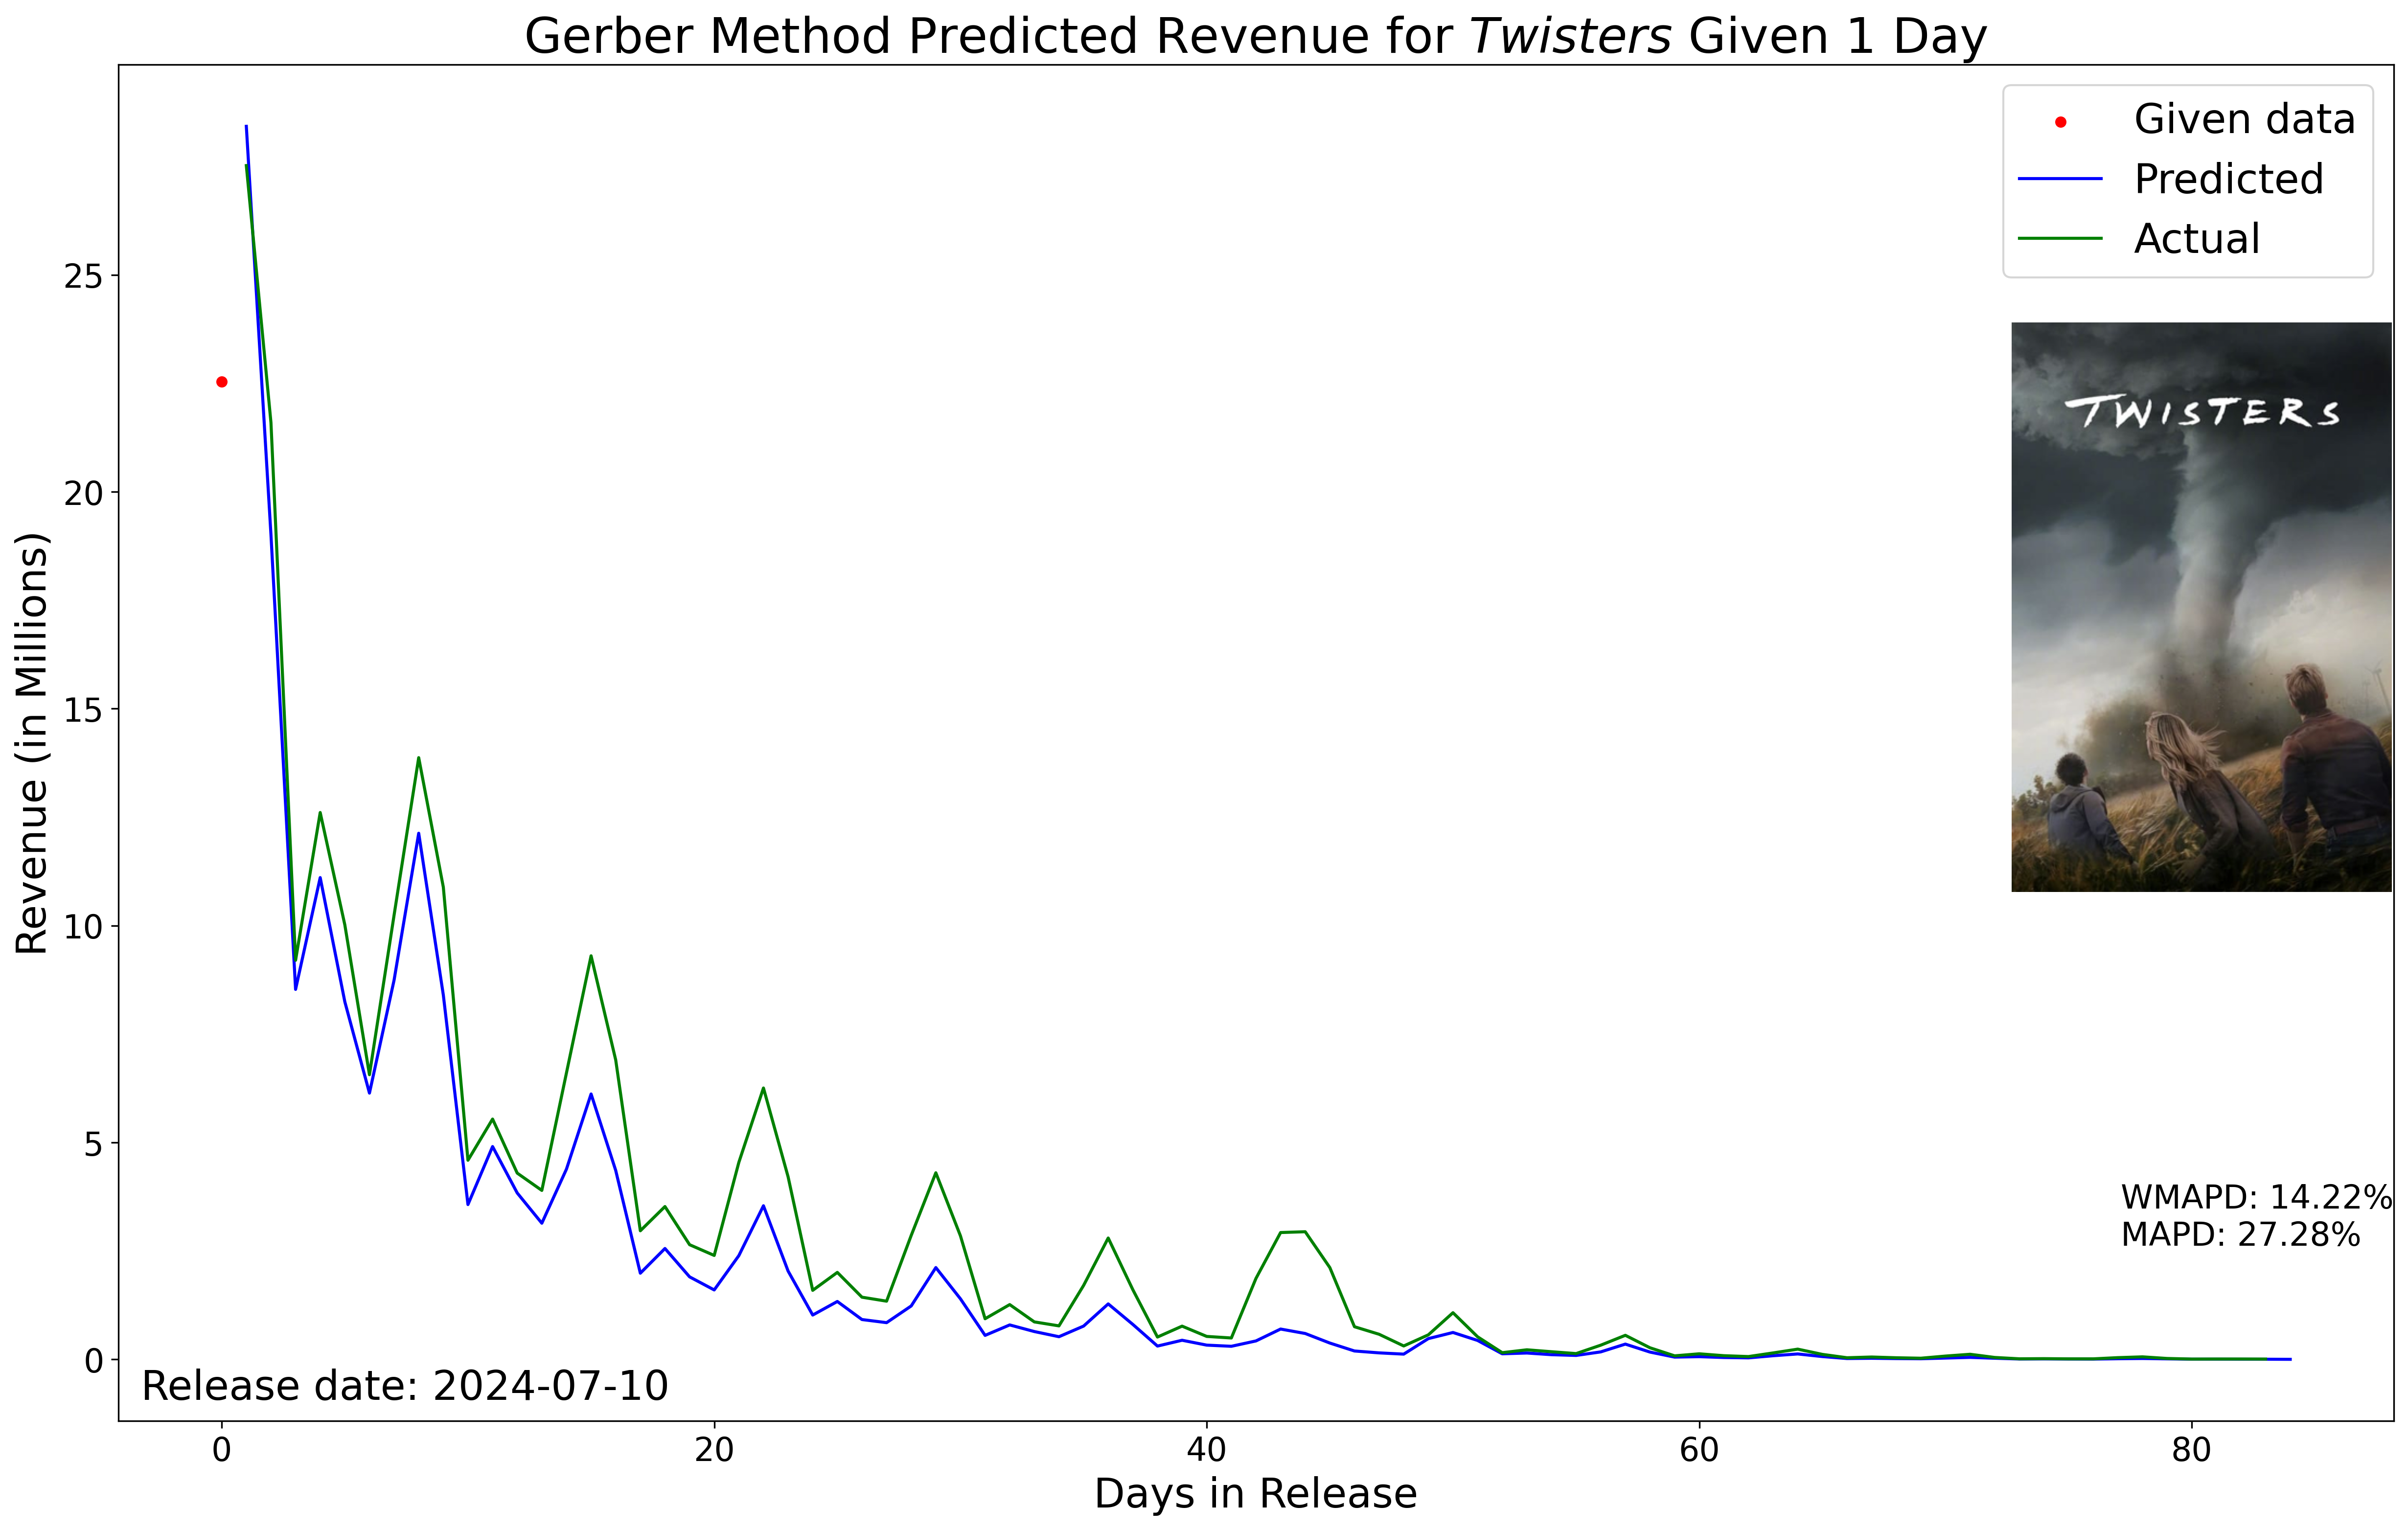
\includegraphics[width=0.95\textwidth]{../shared/images/pred/Twisters_1.png}
  \end{figure}
\end{frame}

\begin{frame}{Metrics}
  \begin{itemize}
    \item MAPD: Mean Absolute Percentage Difference
    \item $\frac{\sum_{i=1}^{n} \frac{|y_i - \hat{y}_i|}{y_i+\hat{y}_i}}{n}$
    \item WMAPD: Weighted Mean Absolute Percentage Difference
    \item $\frac{\sum_{i=1}^{n} | y_i - \hat{y}_i |}{\sum_{i=1}^{n} \left( y_i + \hat{y}_i \right)}$
  \end{itemize}

  \begin{figure}
    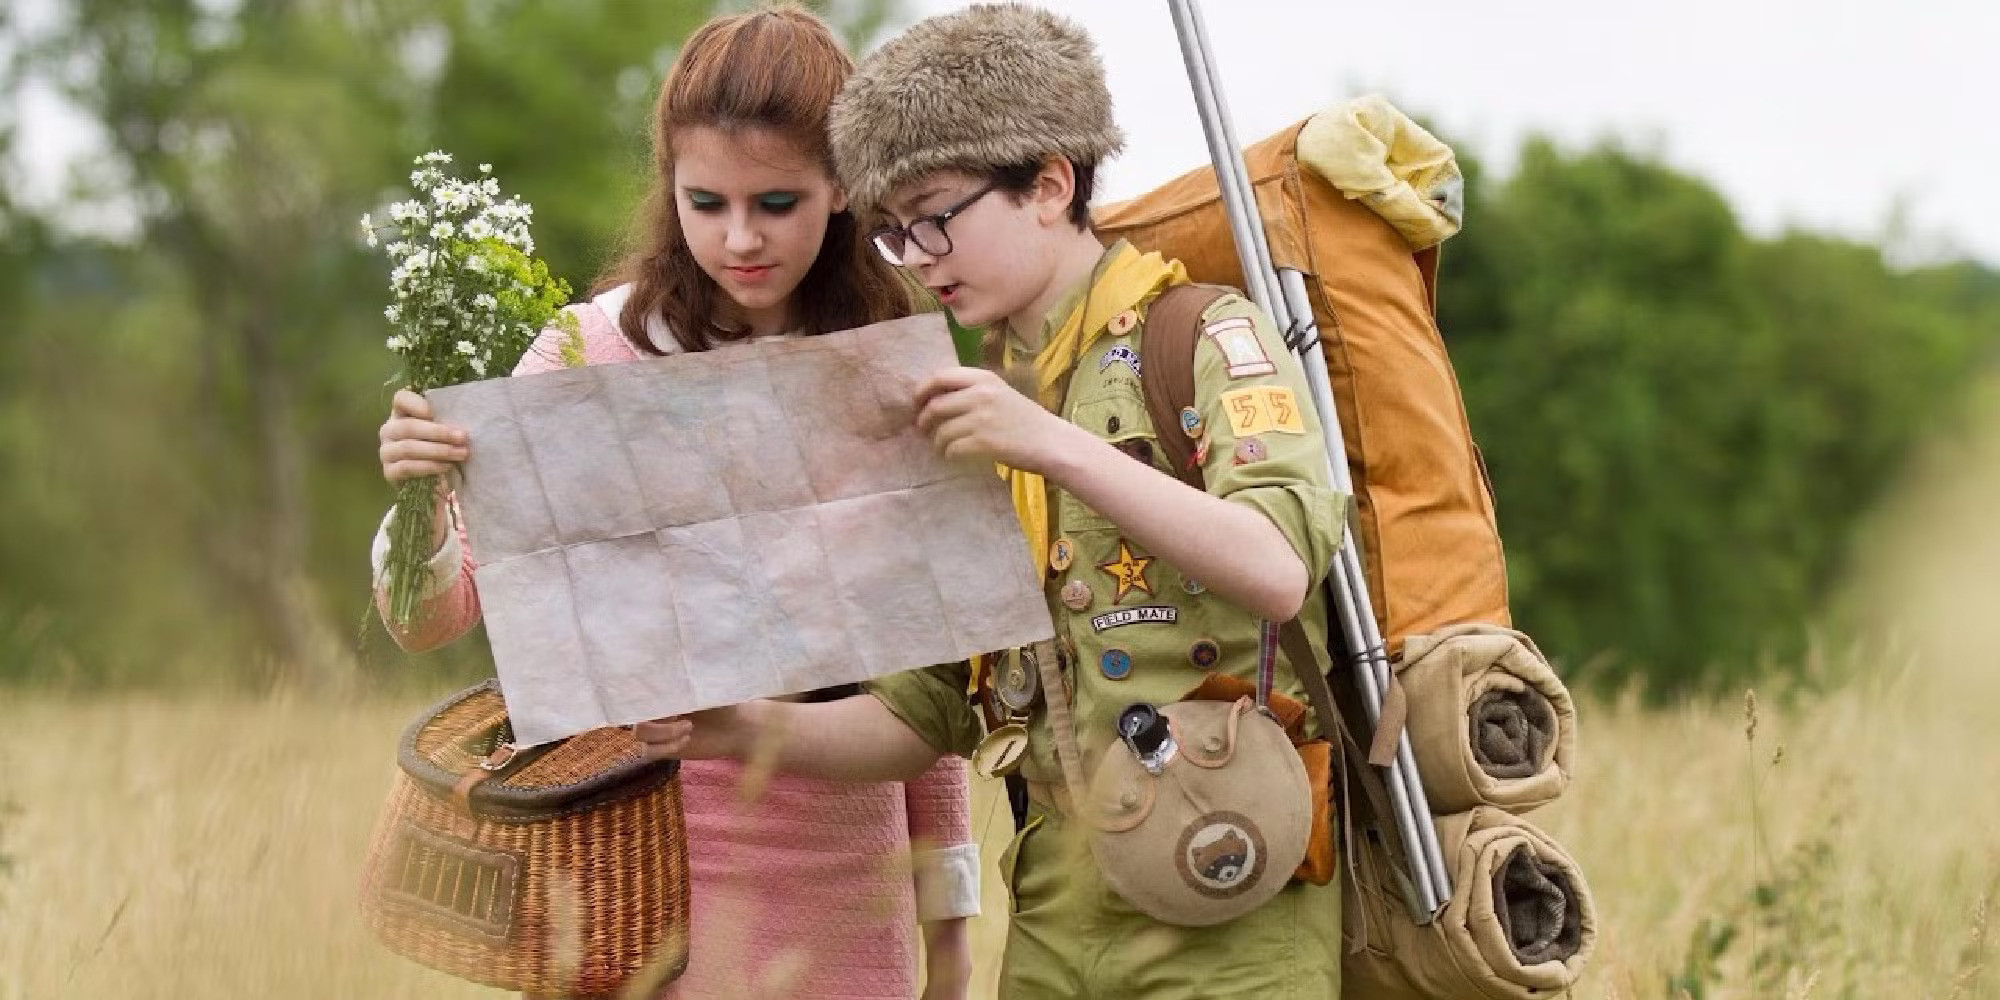
\includegraphics[width=0.6\textwidth]{../shared/images/screenshots/map.jpeg}
  \end{figure}
\end{frame}

\begin{frame}{Results: \cite{monkeyMan}}
  \begin{figure}
    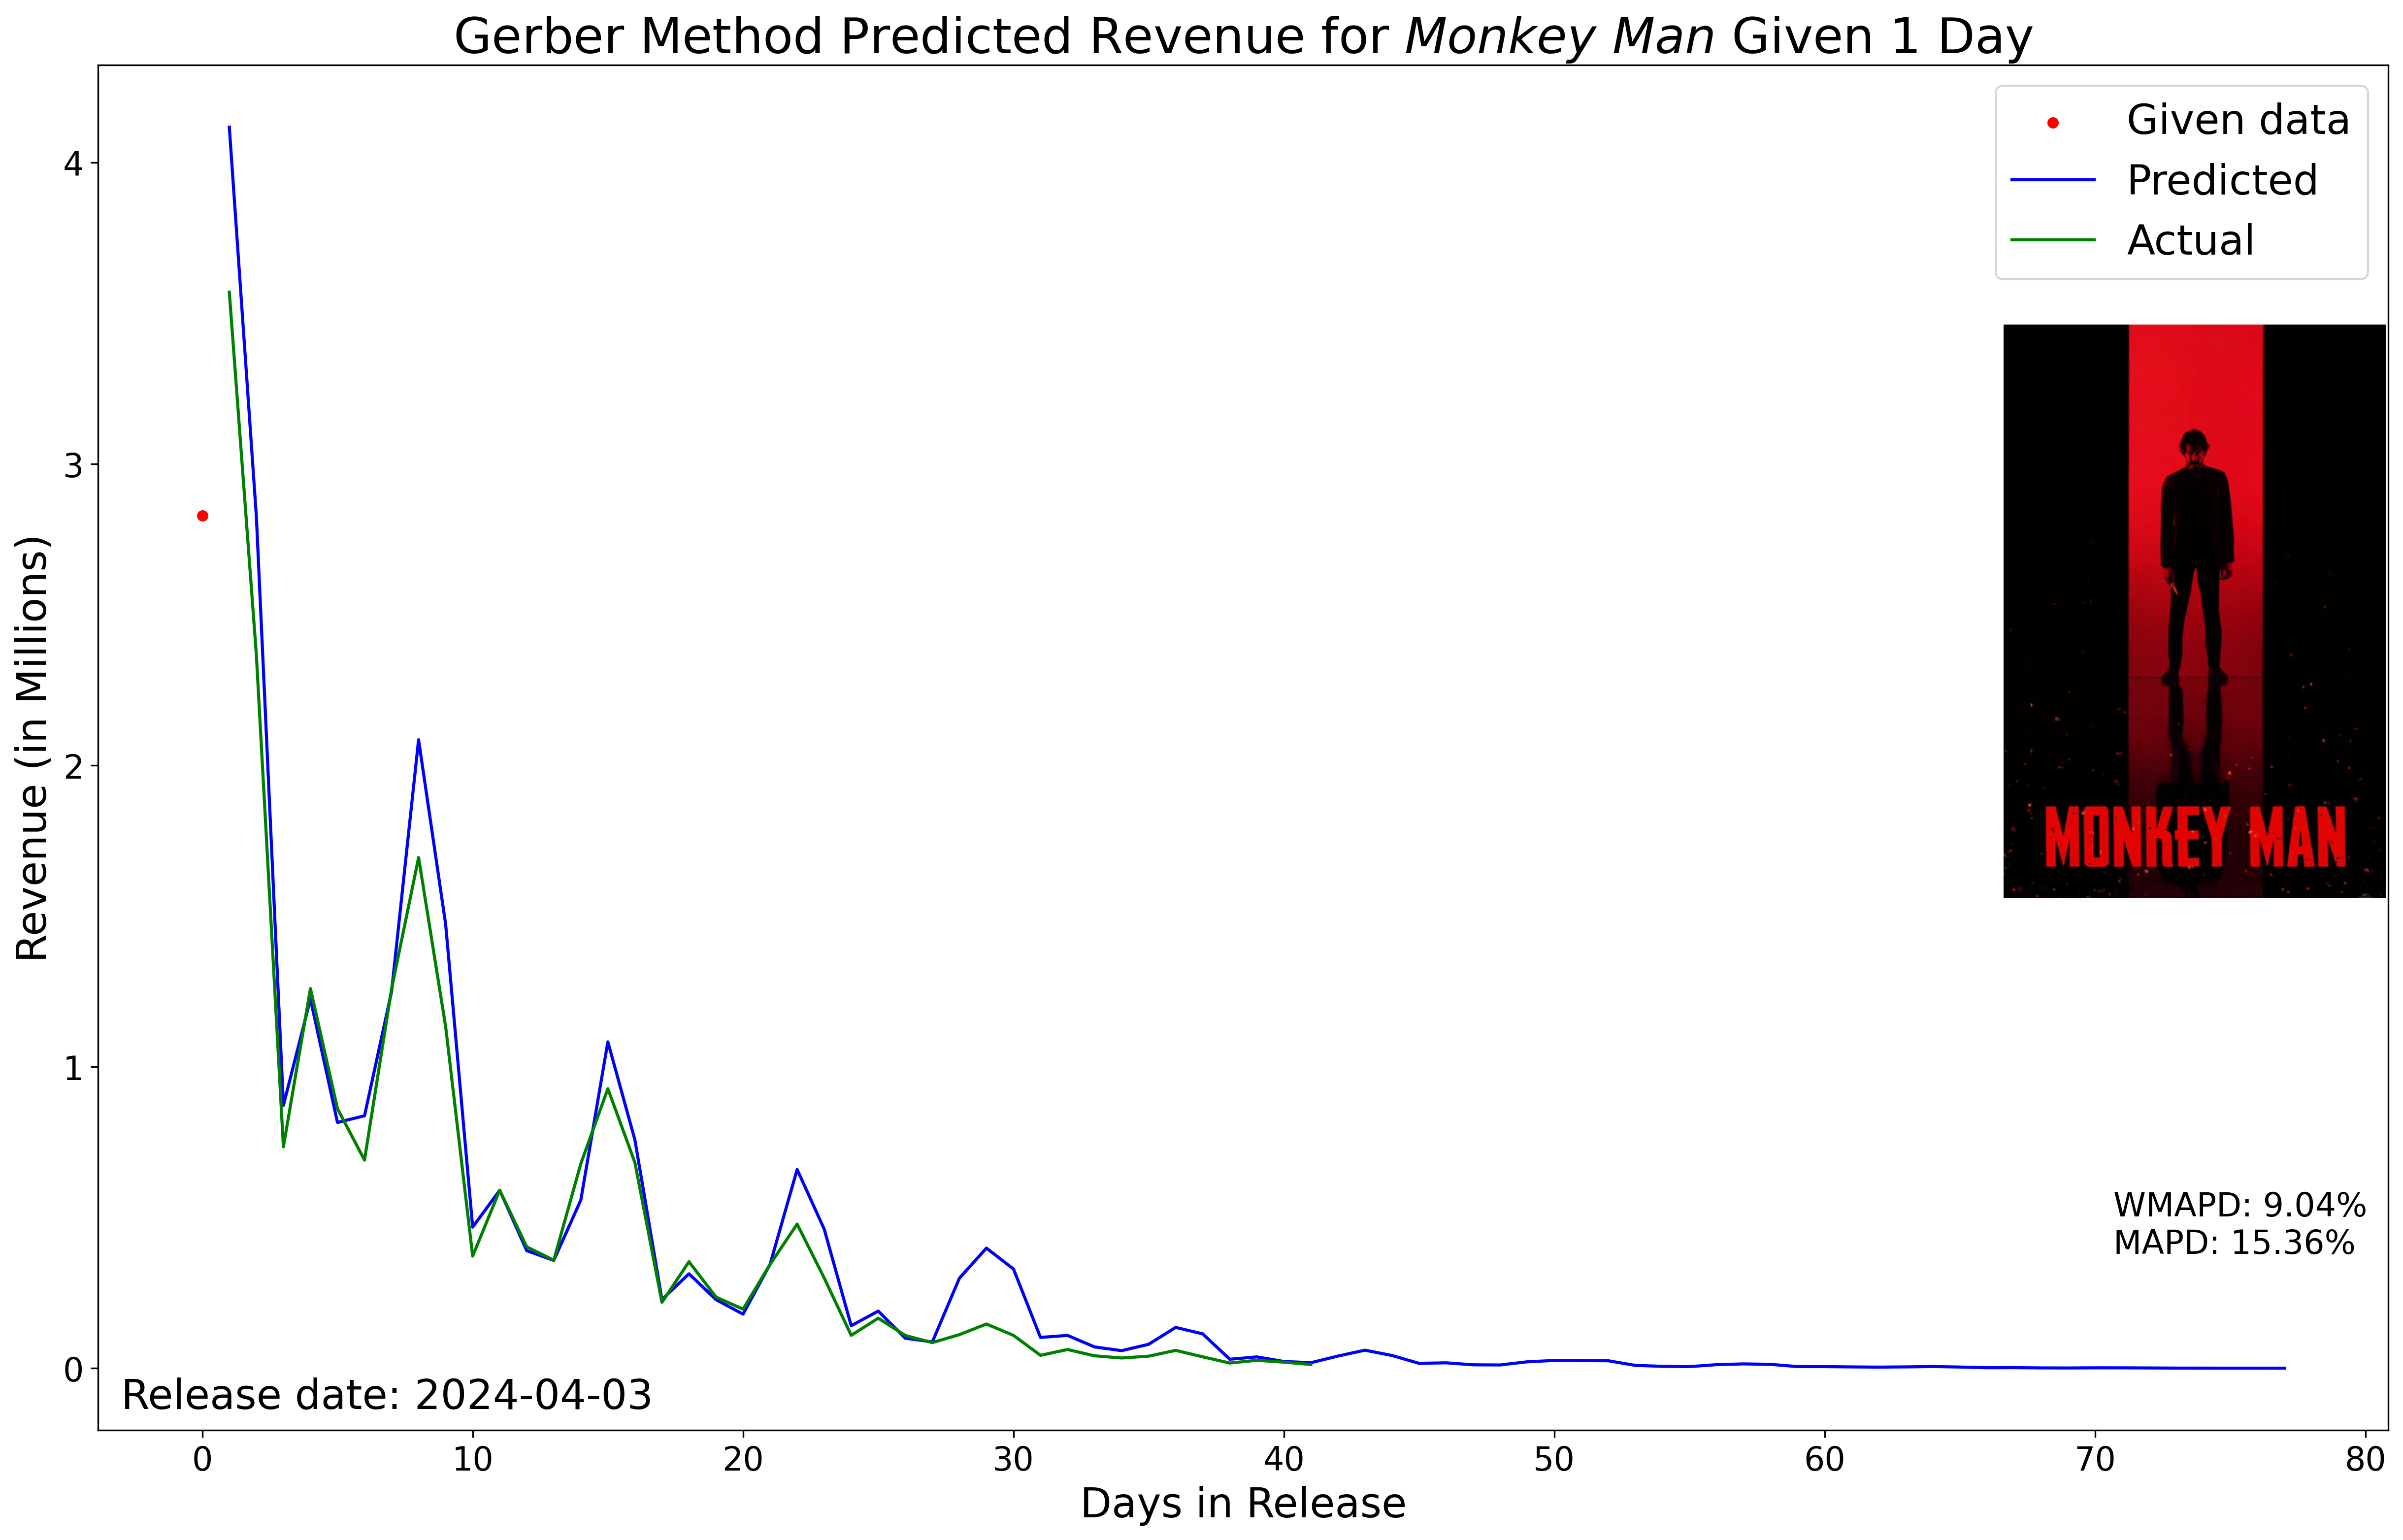
\includegraphics[width=0.95\textwidth]{../shared/images/pred/Monkey Man_1.png}
  \end{figure}
\end{frame}

\begin{frame}{Opening Day Predictions}
  \begin{tikzpicture}[remember picture, overlay]
    \node[below left] at (current page.north east) 
    {
        
\includegraphics[width=0.47\textwidth]{../shared/images/screenshots/training.jpg}
    };
  \end{tikzpicture}
    
  \begin{itemize}
    \item Train a \textit{robust multiple linear \newline regression} to predict opening day
    \item Based on budget, Wikipedia page views, YouTube trailer views, and whether a movie is in a franchise
    \item $R^2$ of 0.47
  \end{itemize}

  \begin{figure}
    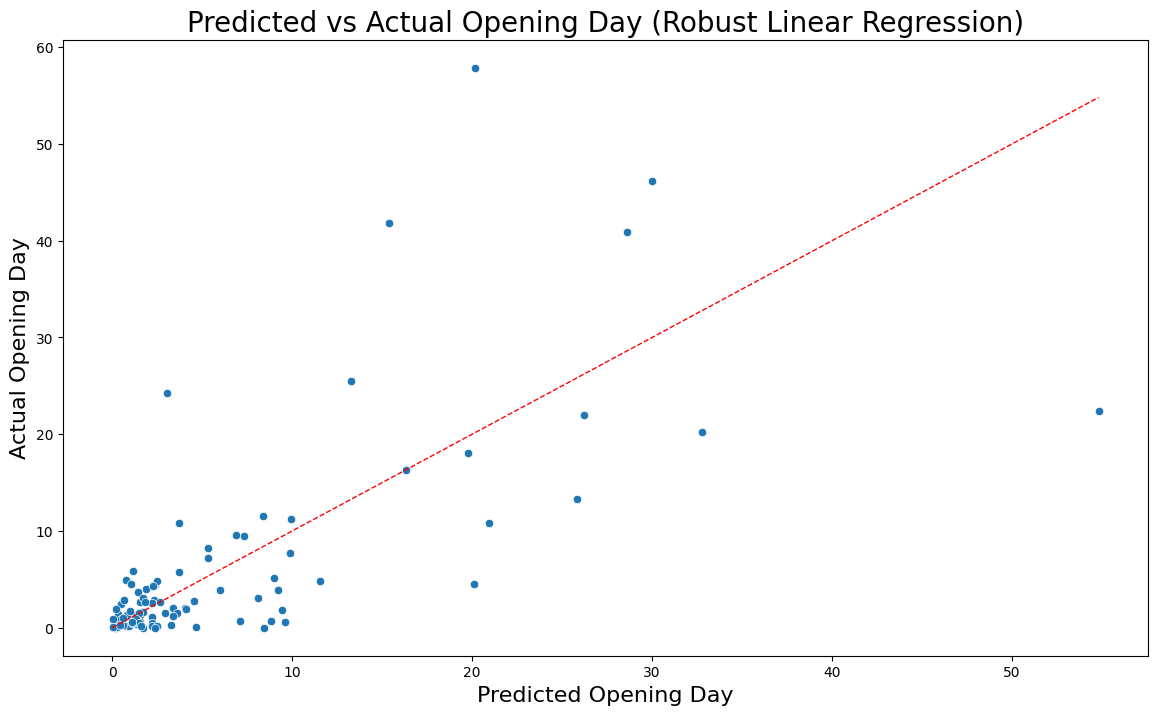
\includegraphics[width=0.55\textwidth]{../shared/images/openingdaypred.png}
  \end{figure}
\end{frame}

% mean girls results multi
\begin{frame}{Results Multiple: \cite{meanGirls}}
  \begin{figure}
    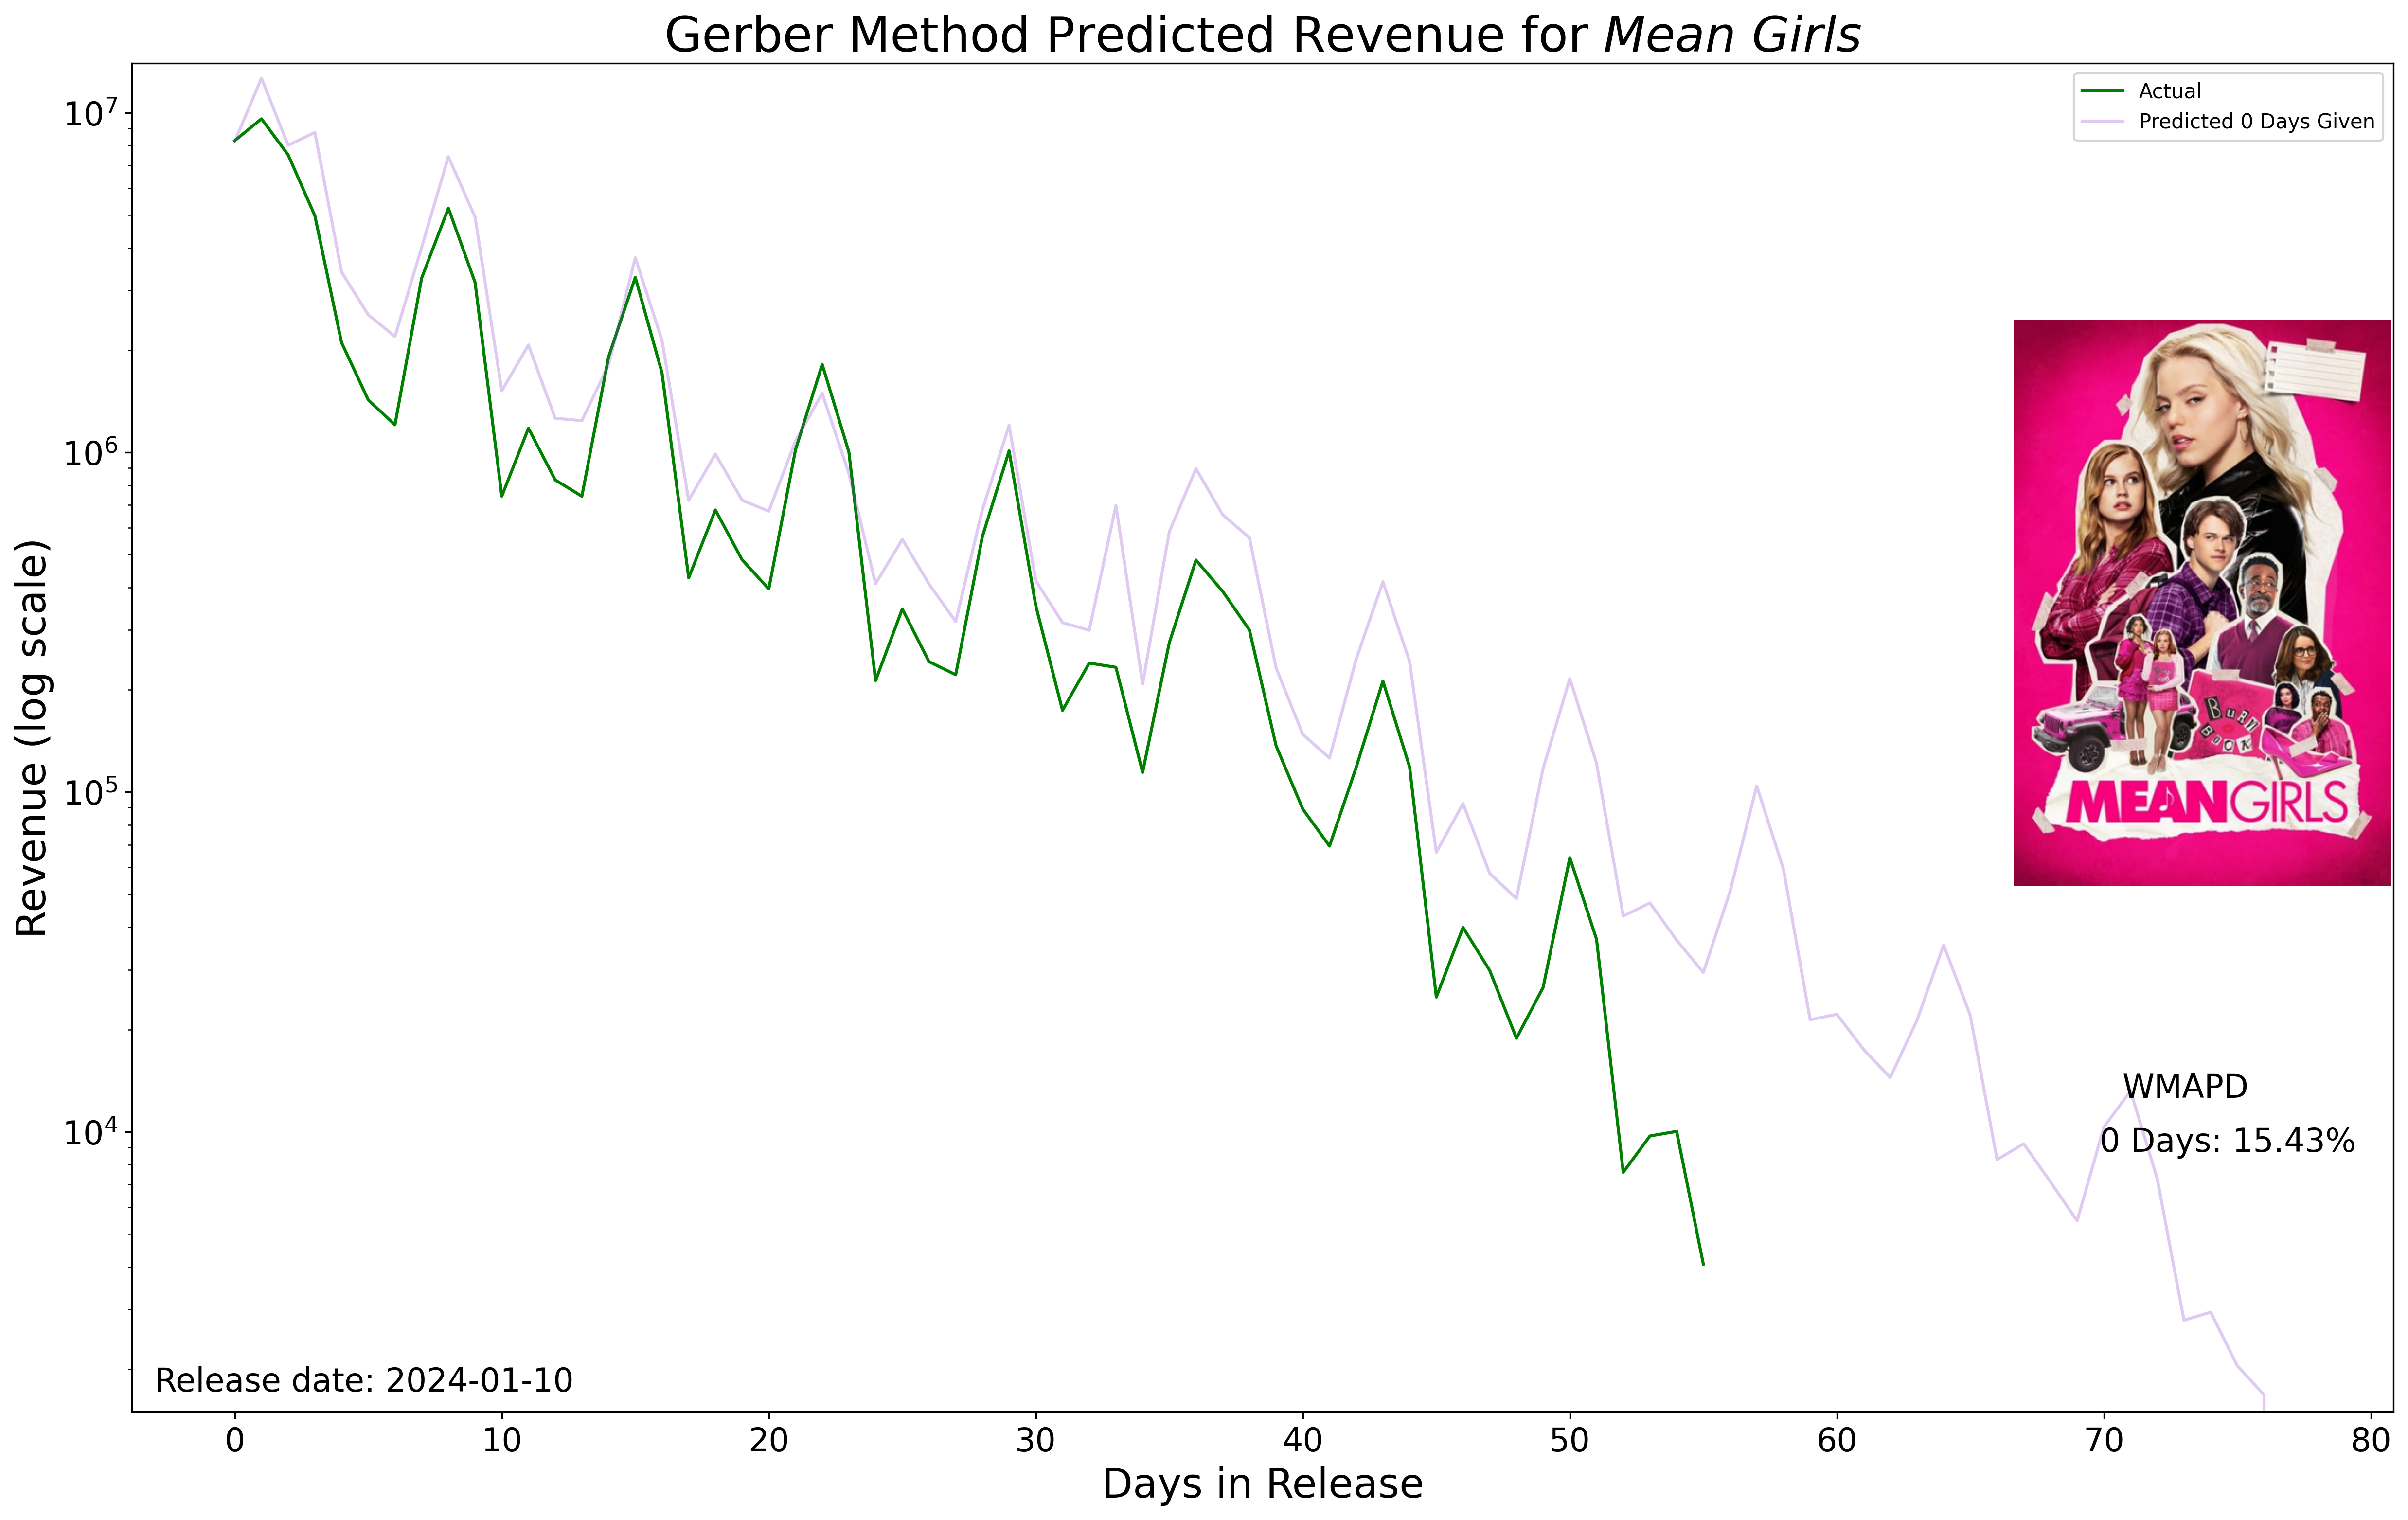
\includegraphics[width=0.95\textwidth]{../shared/images/pred/Mean Girls_multiple_1.png}
  \end{figure}
\end{frame}

\begin{frame}{Results Multiple: \cite{meanGirls}}
  \begin{figure}
    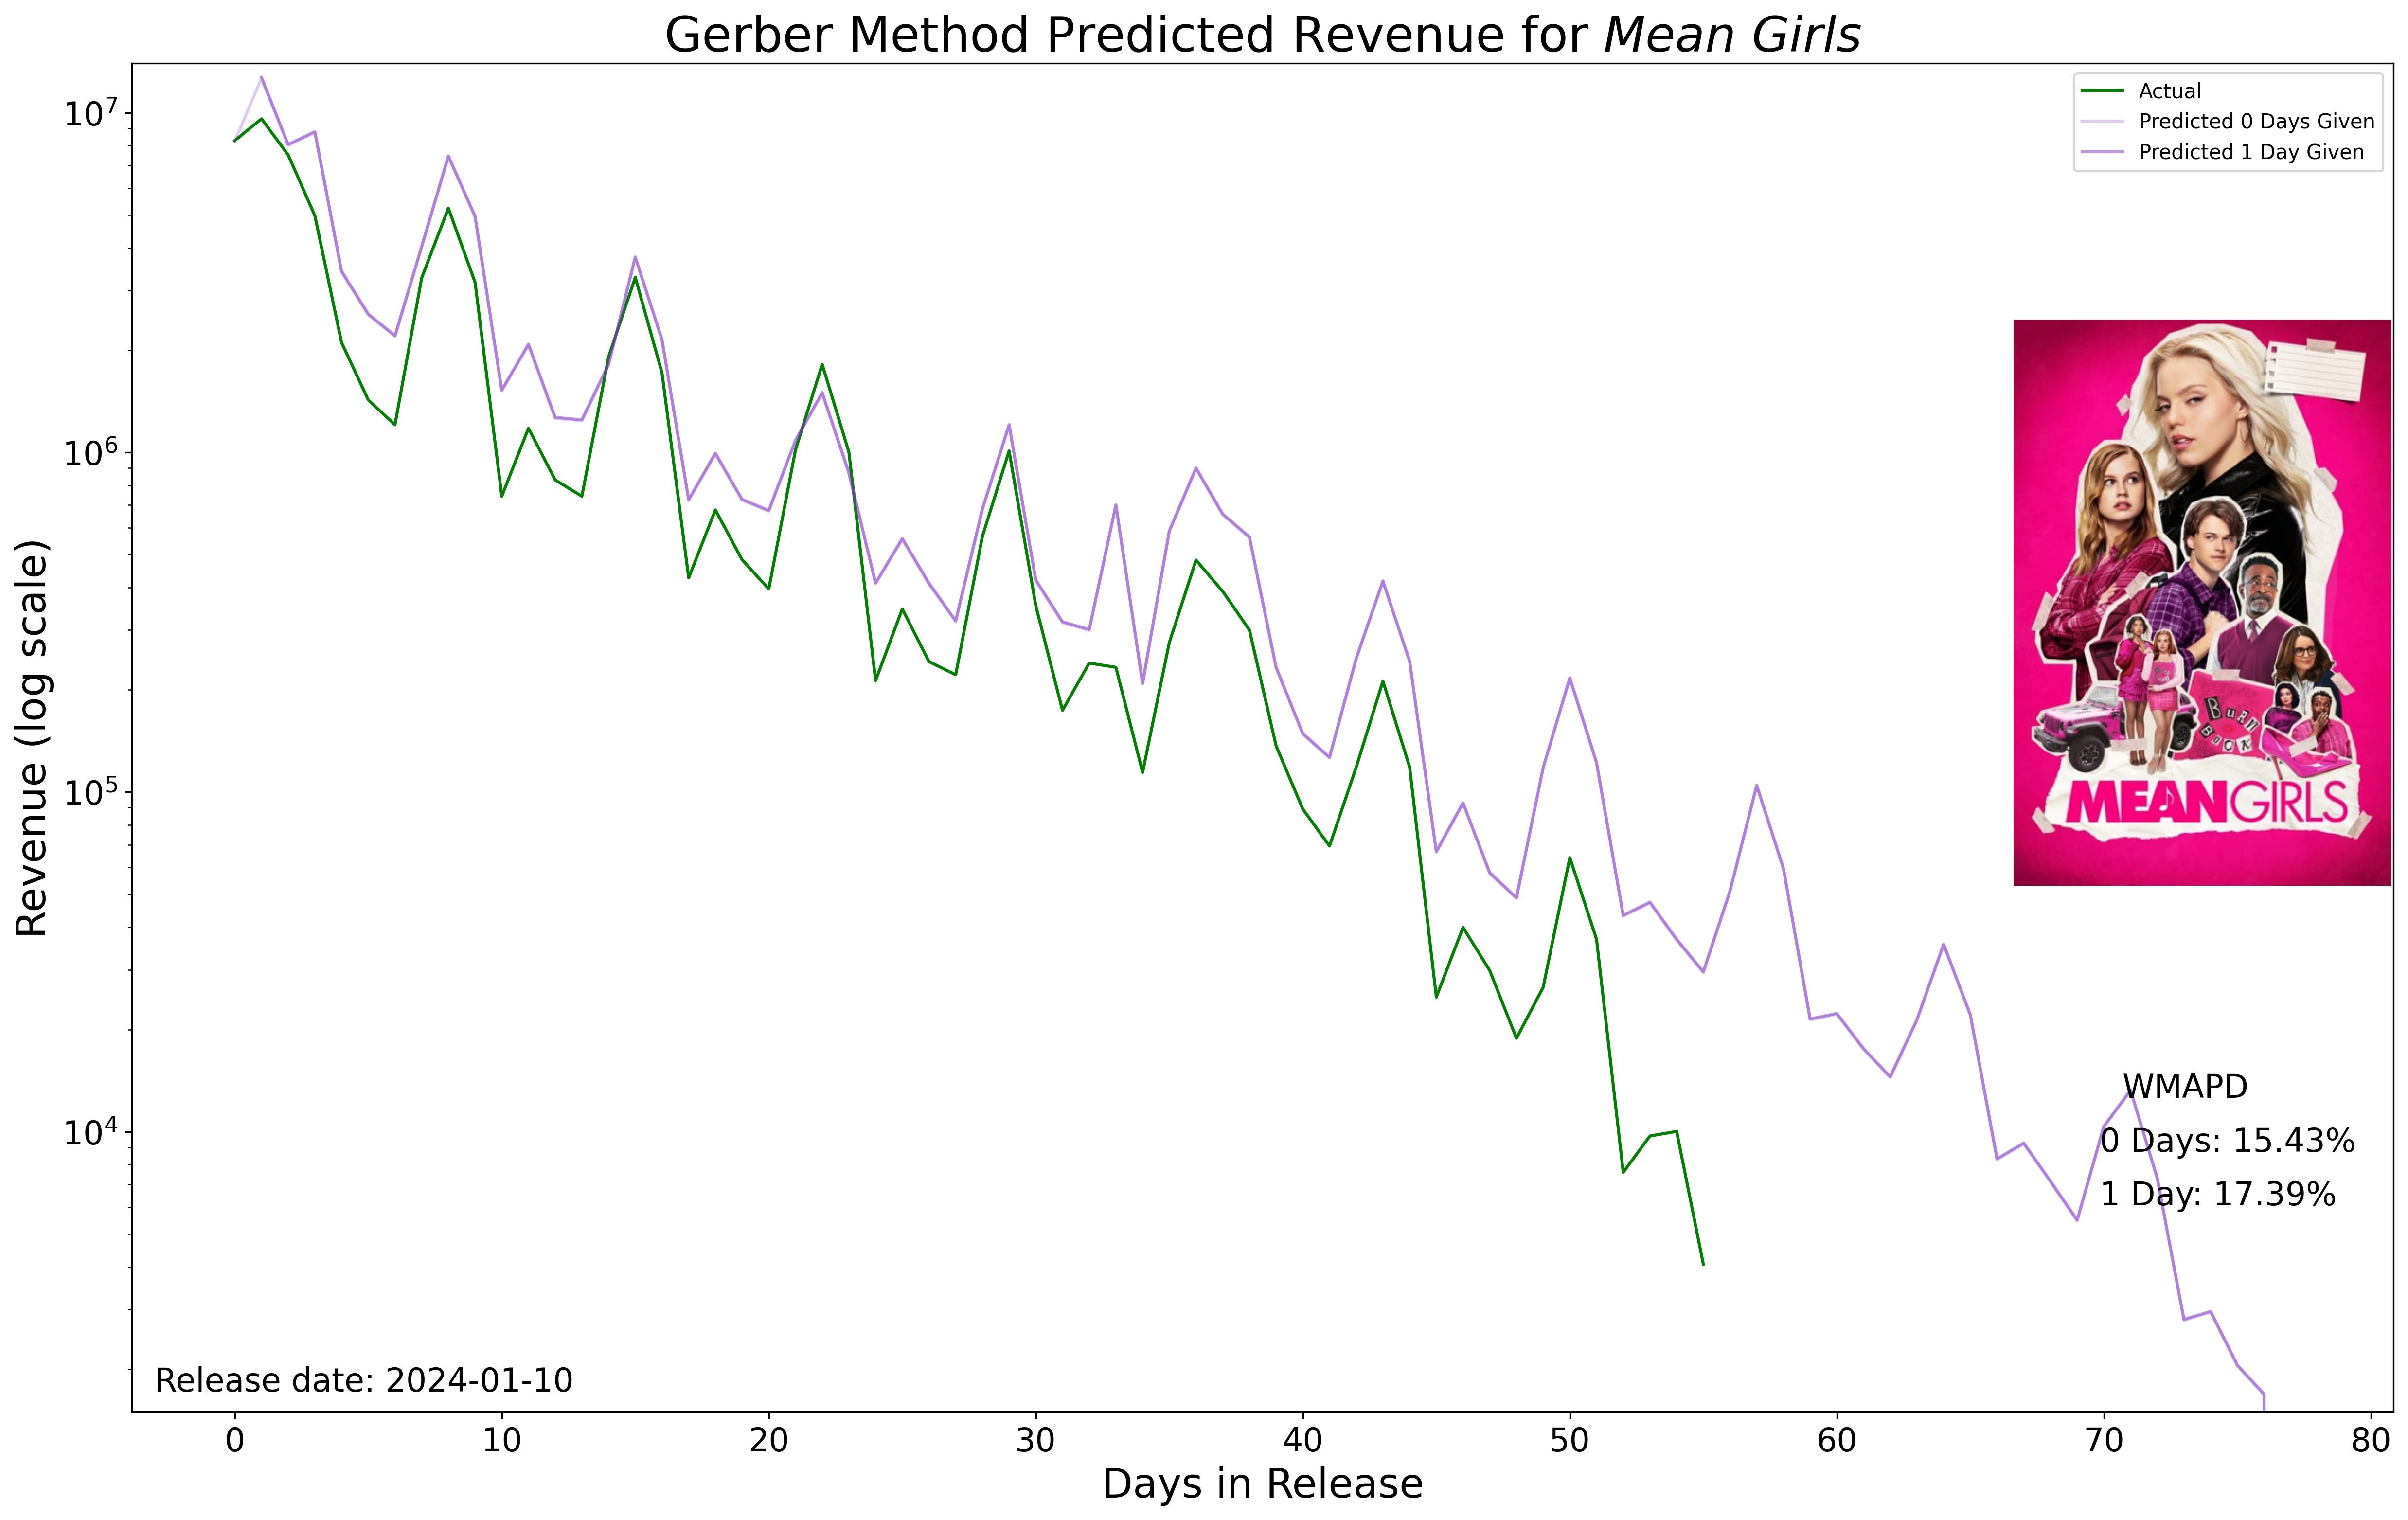
\includegraphics[width=0.95\textwidth]{../shared/images/pred/Mean Girls_multiple_2.png}
  \end{figure}
  \addtocounter{framenumber}{-1}
\end{frame}

\begin{frame}{Results Multiple: \cite{meanGirls}}
  \begin{figure}
    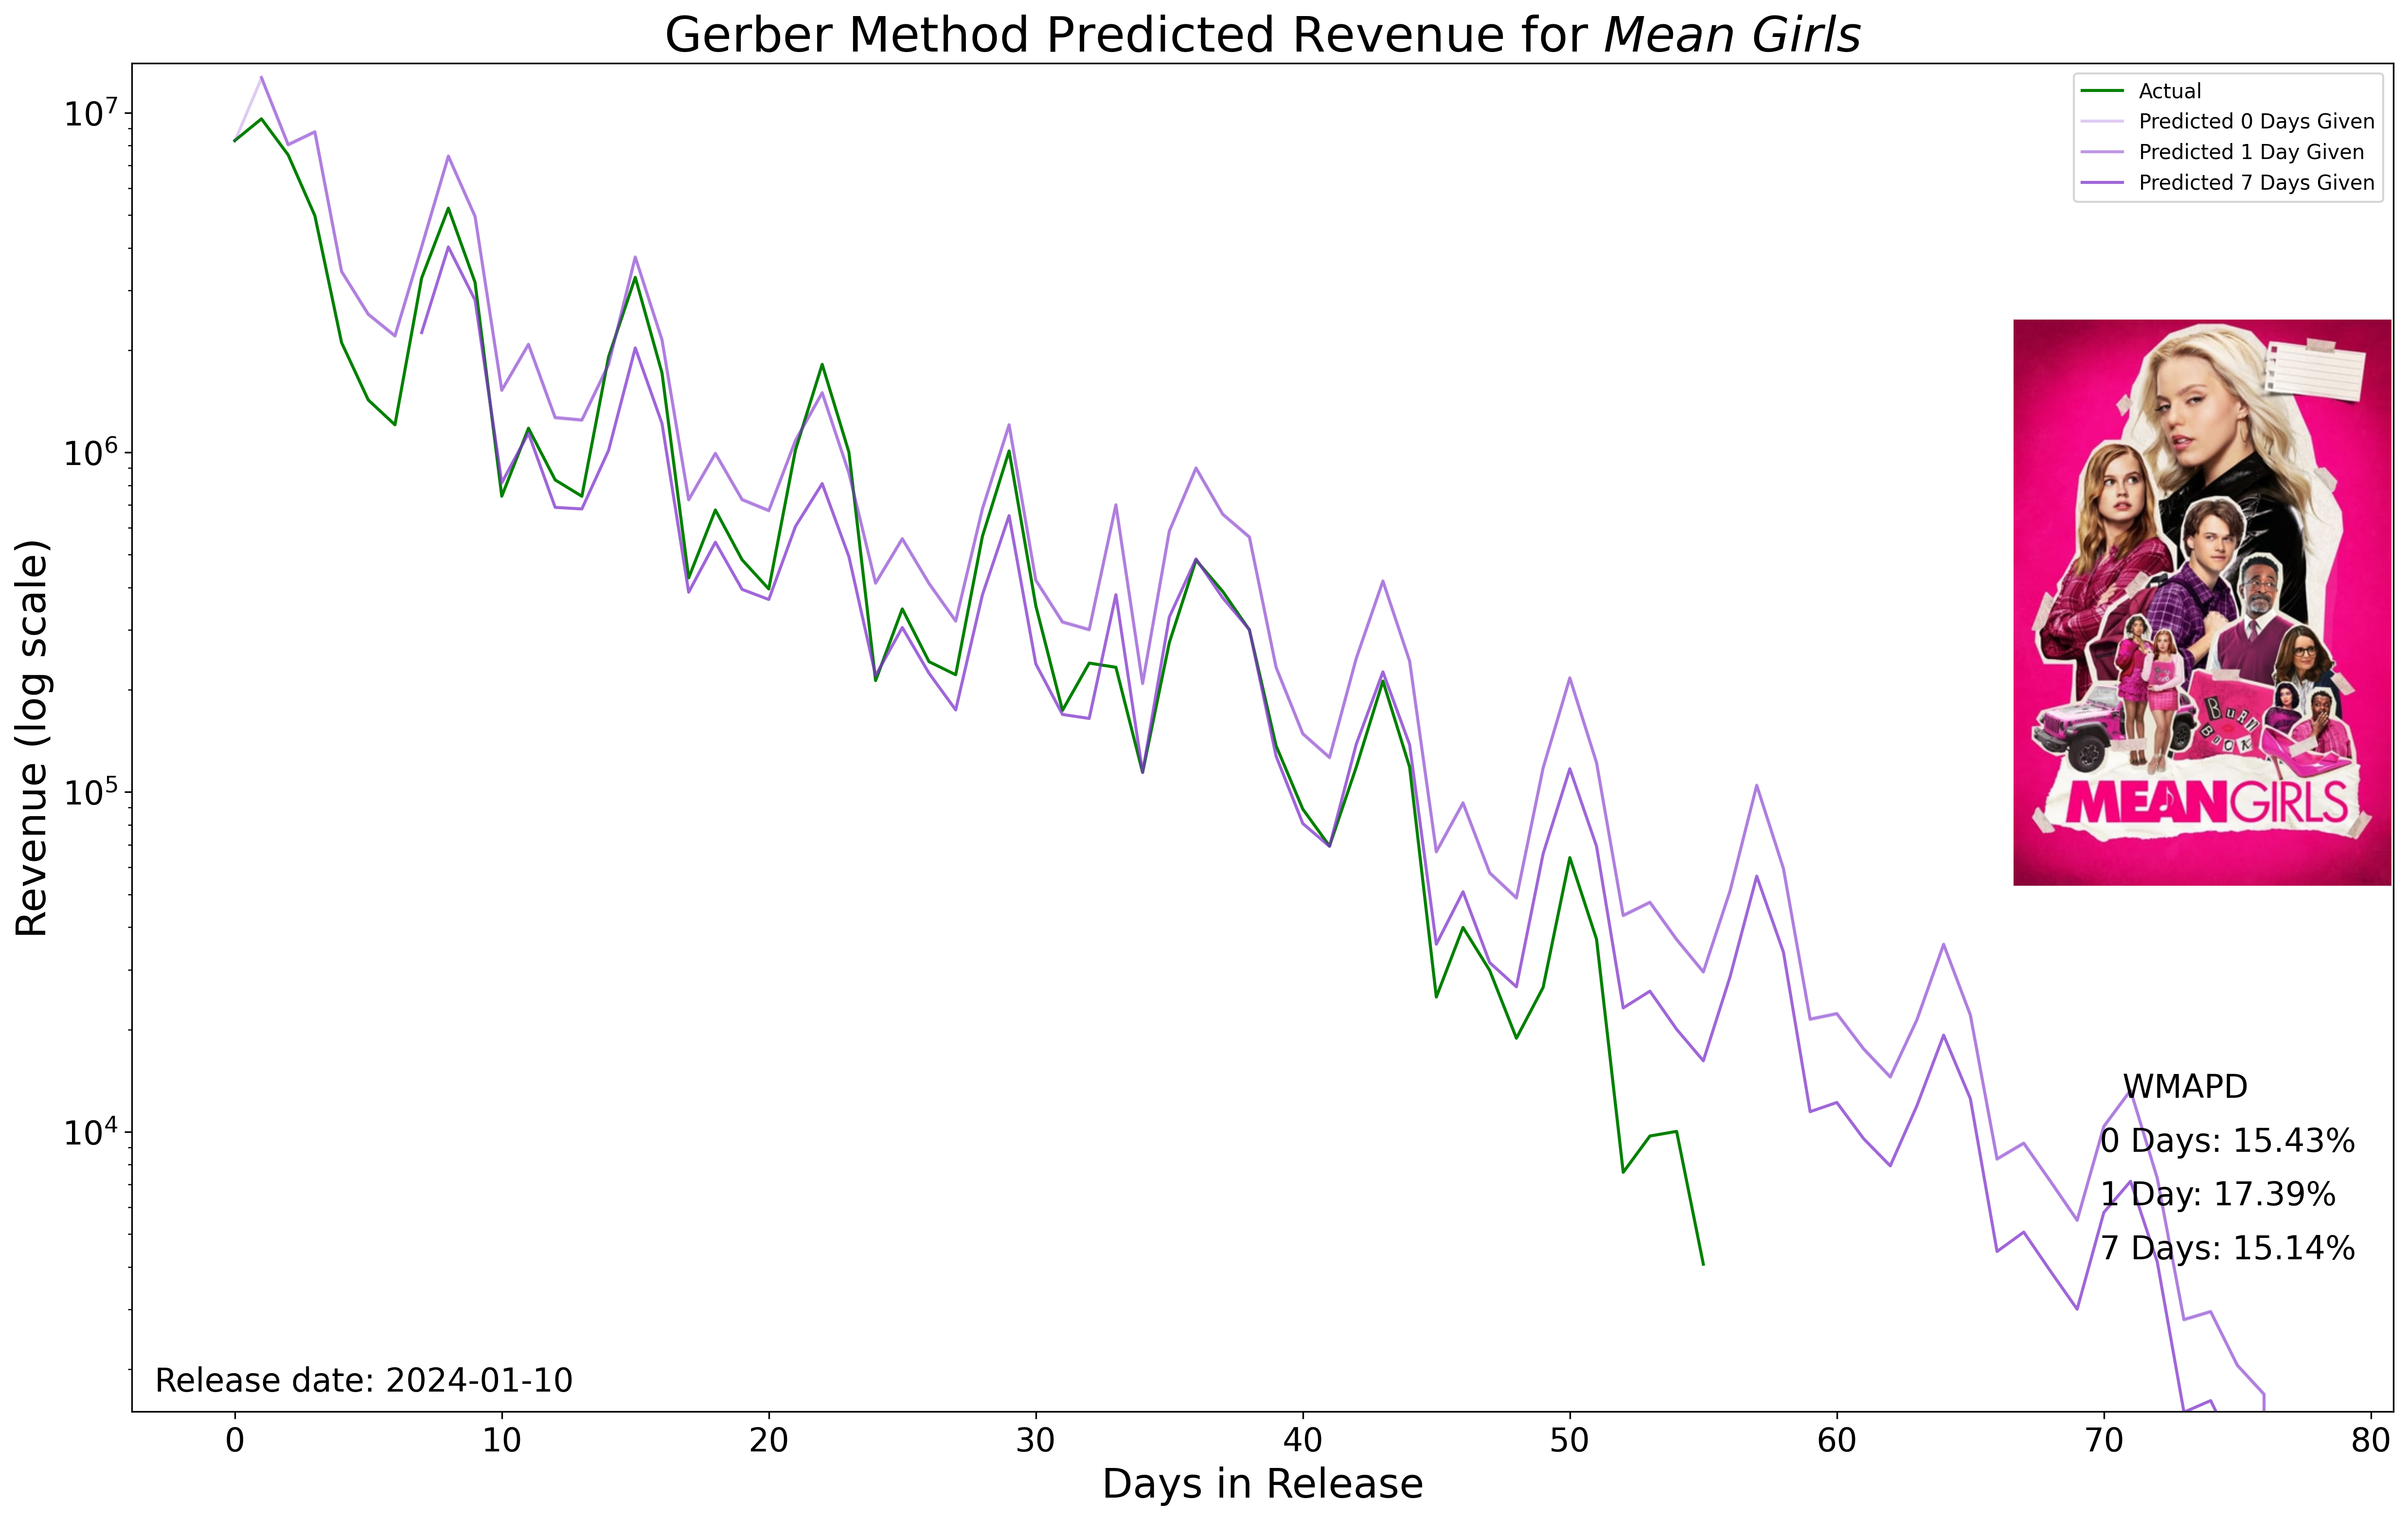
\includegraphics[width=0.95\textwidth]{../shared/images/pred/Mean Girls_multiple_3.png}
  \end{figure}
  \addtocounter{framenumber}{-1}
\end{frame}

\begin{frame}{Results Multiple: \cite{meanGirls}}
  \begin{figure}
    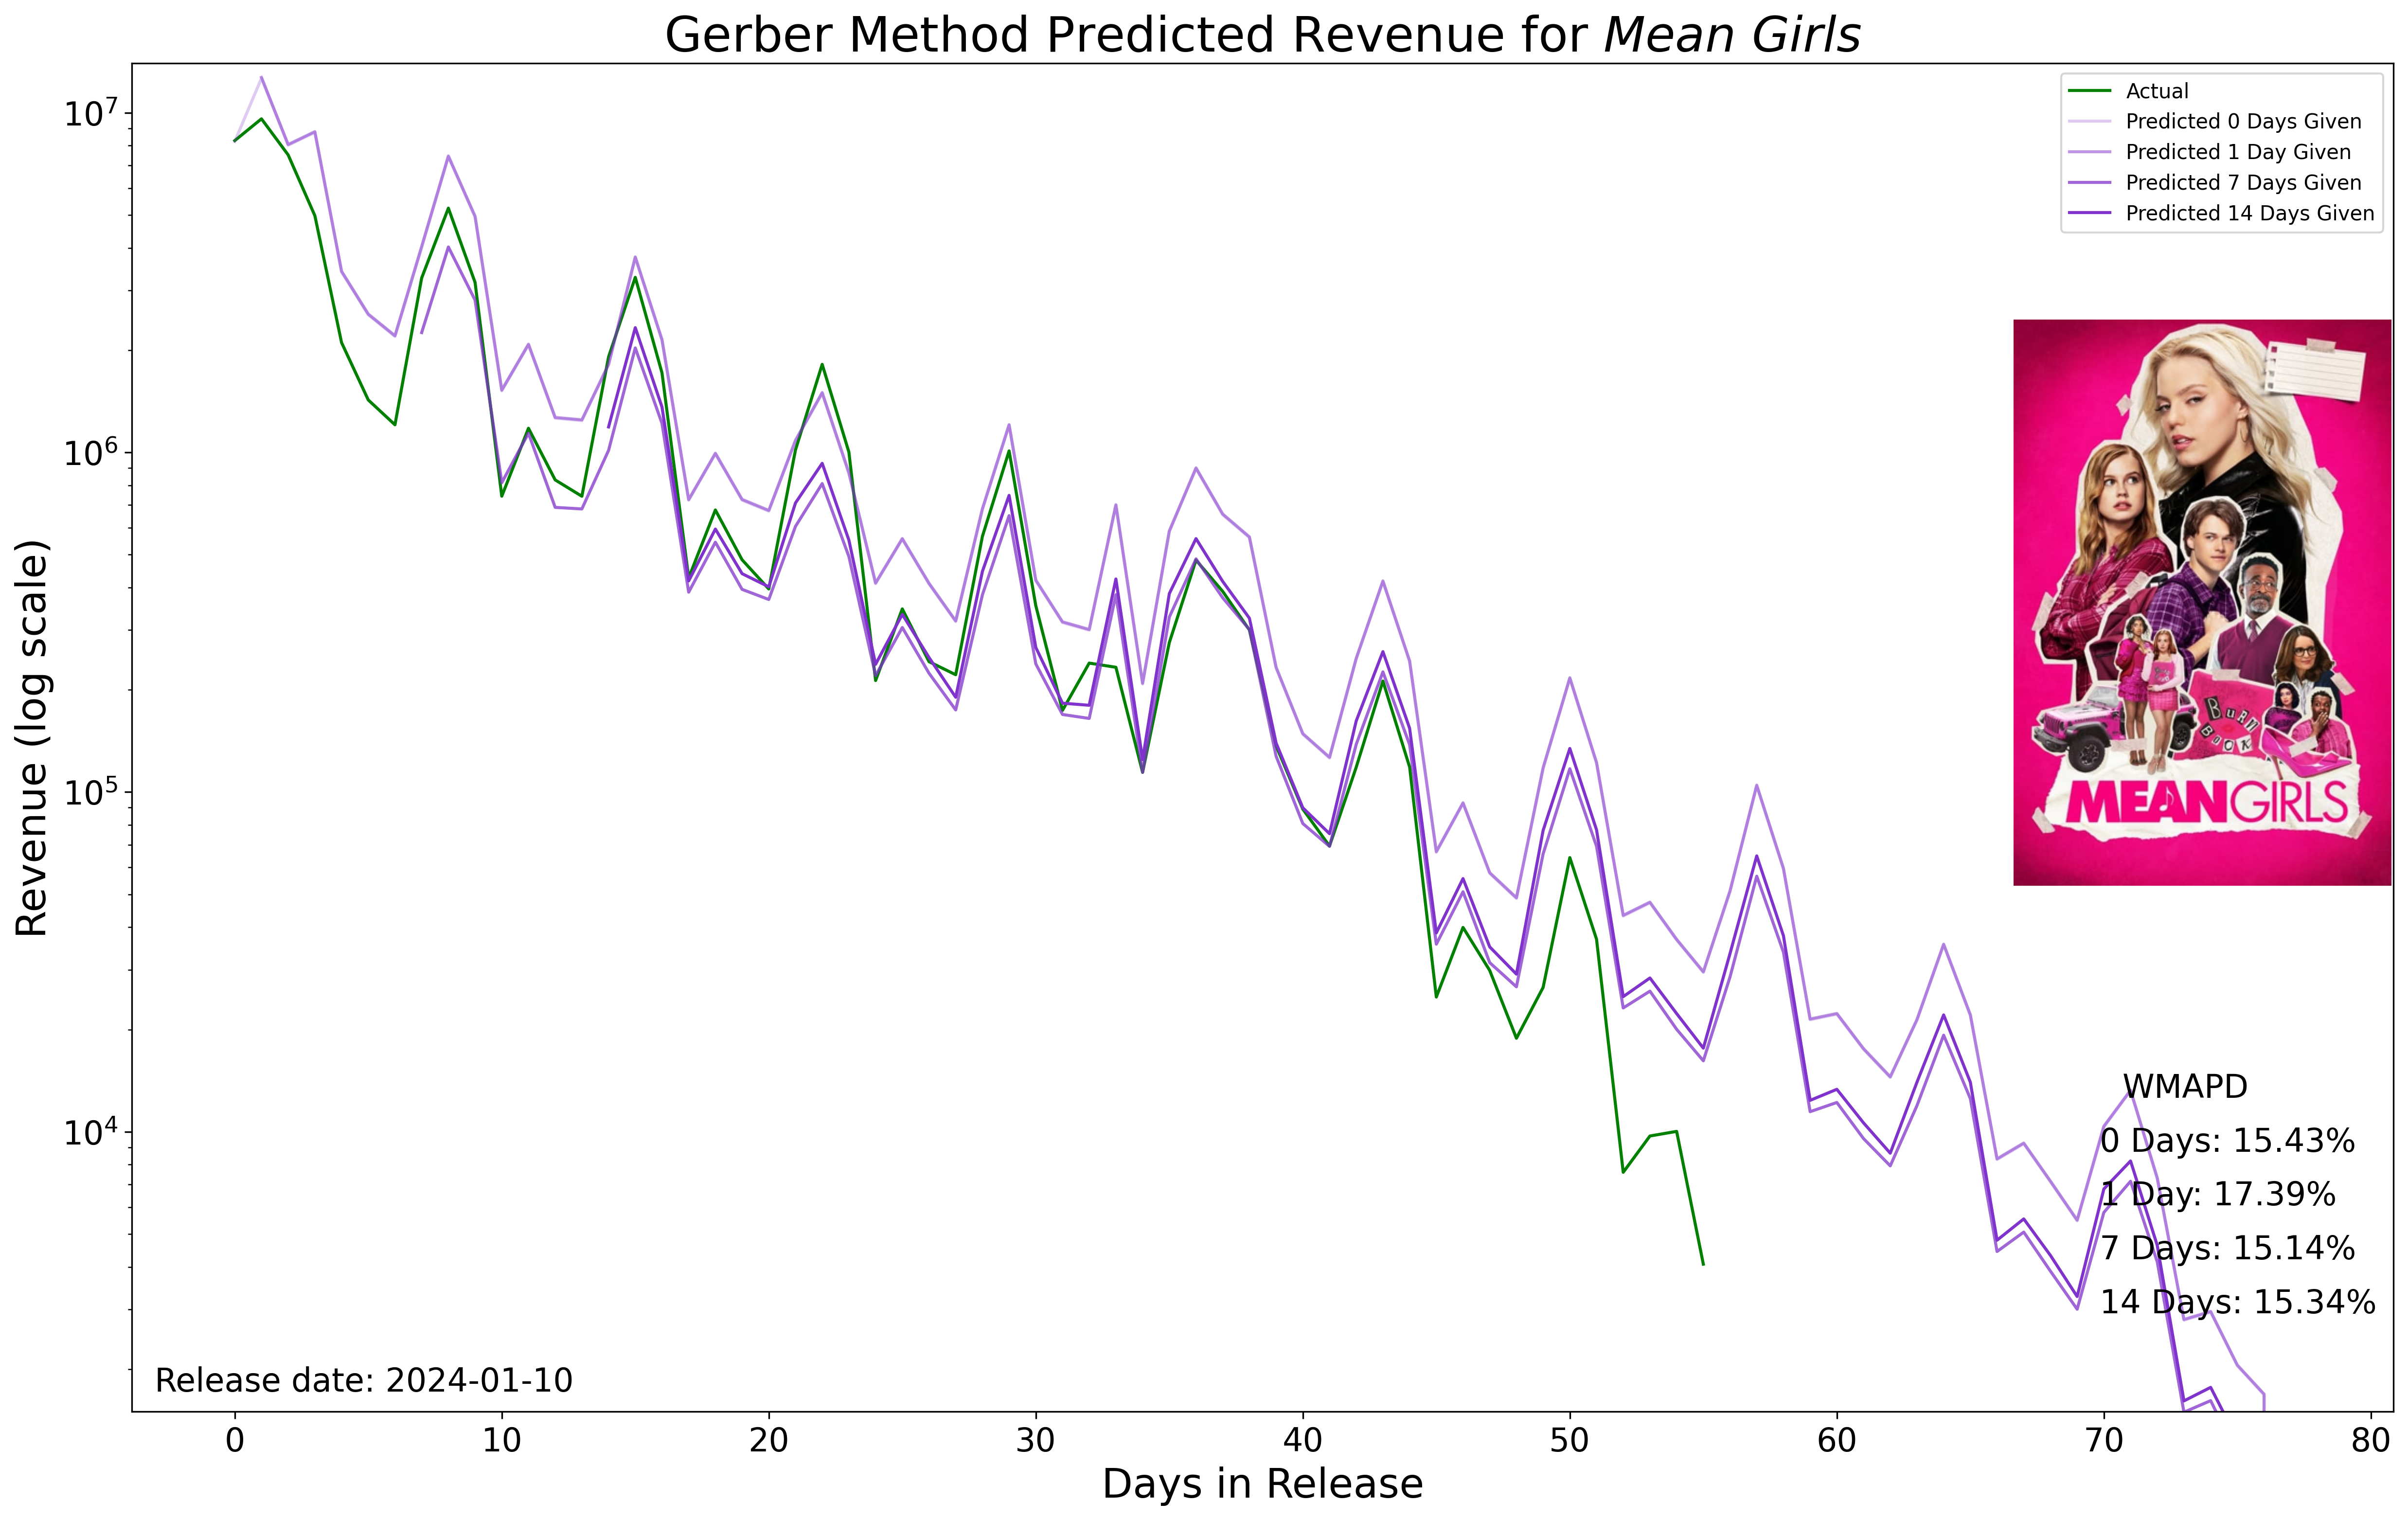
\includegraphics[width=0.95\textwidth]{../shared/images/pred/Mean Girls_multiple_4.png}
  \end{figure}
  \addtocounter{framenumber}{-1}
\end{frame}

\begin{frame}{Results Multiple: \cite{jokerFolie}}
  \begin{figure}
    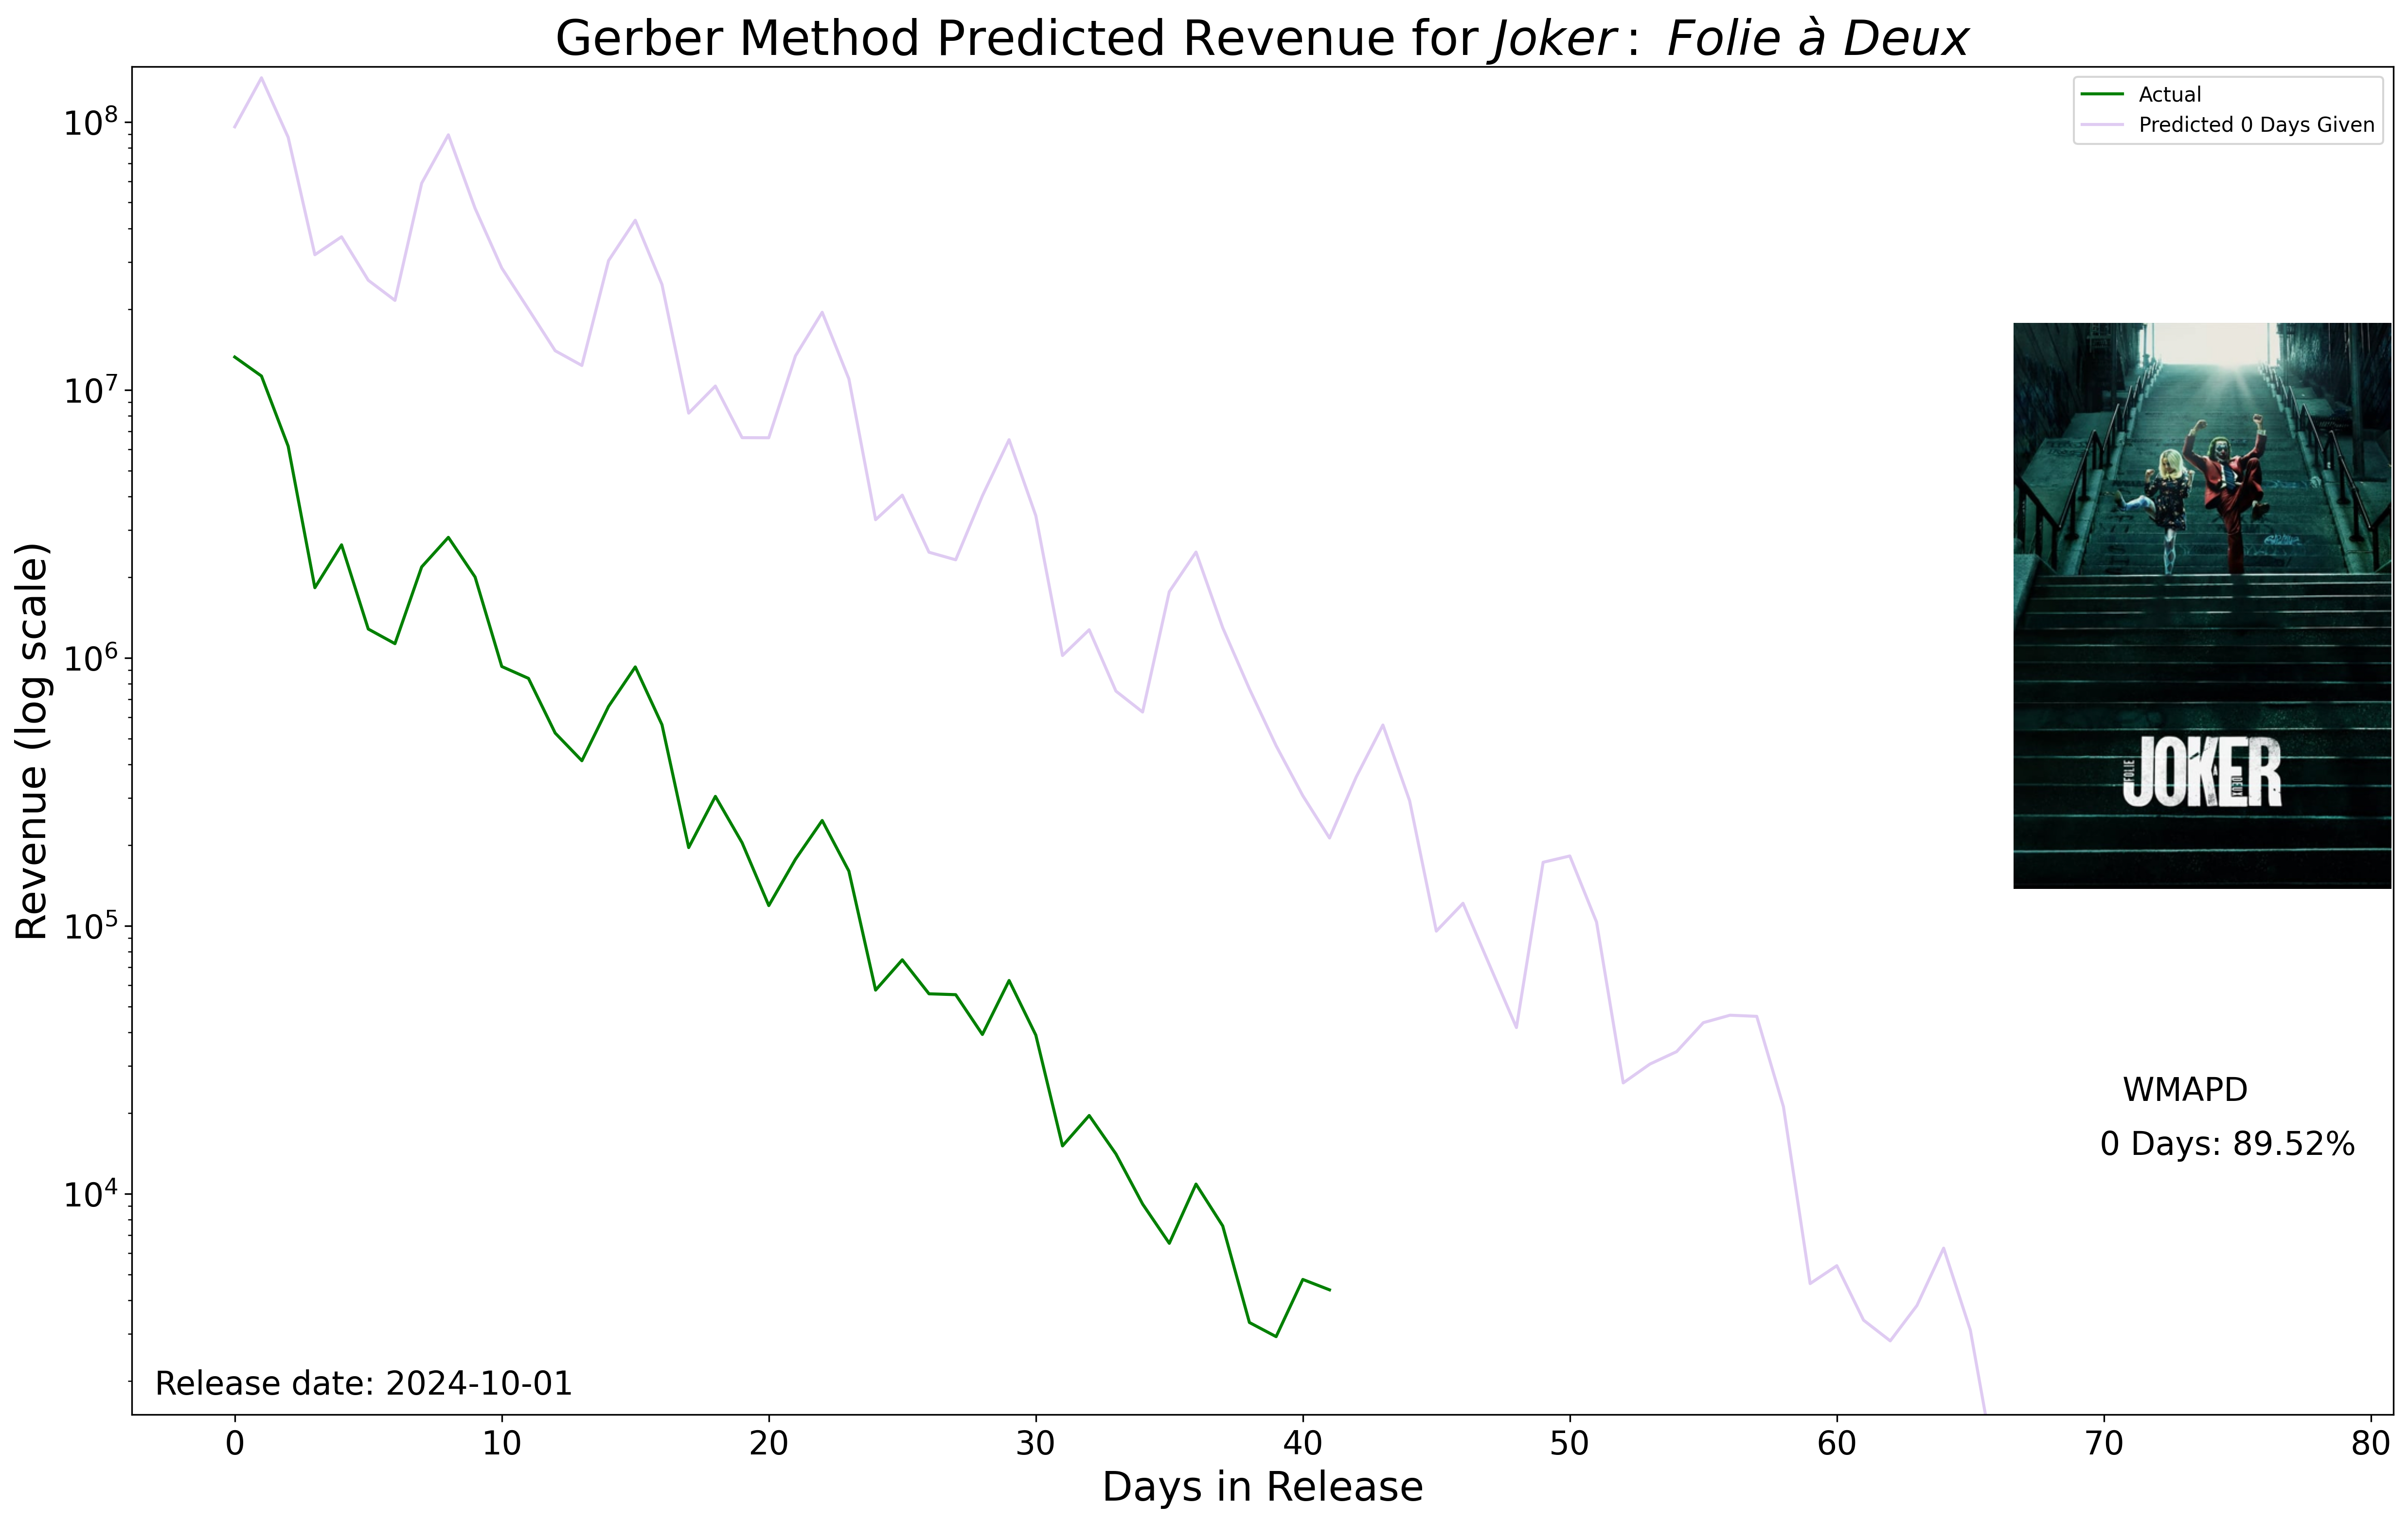
\includegraphics[width=0.95\textwidth]{../shared/images/pred/Joker: Folie à Deux_multiple_1.png}
  \end{figure}
\end{frame}

\begin{frame}{Results Multiple: \cite{jokerFolie}}
  \begin{figure}
    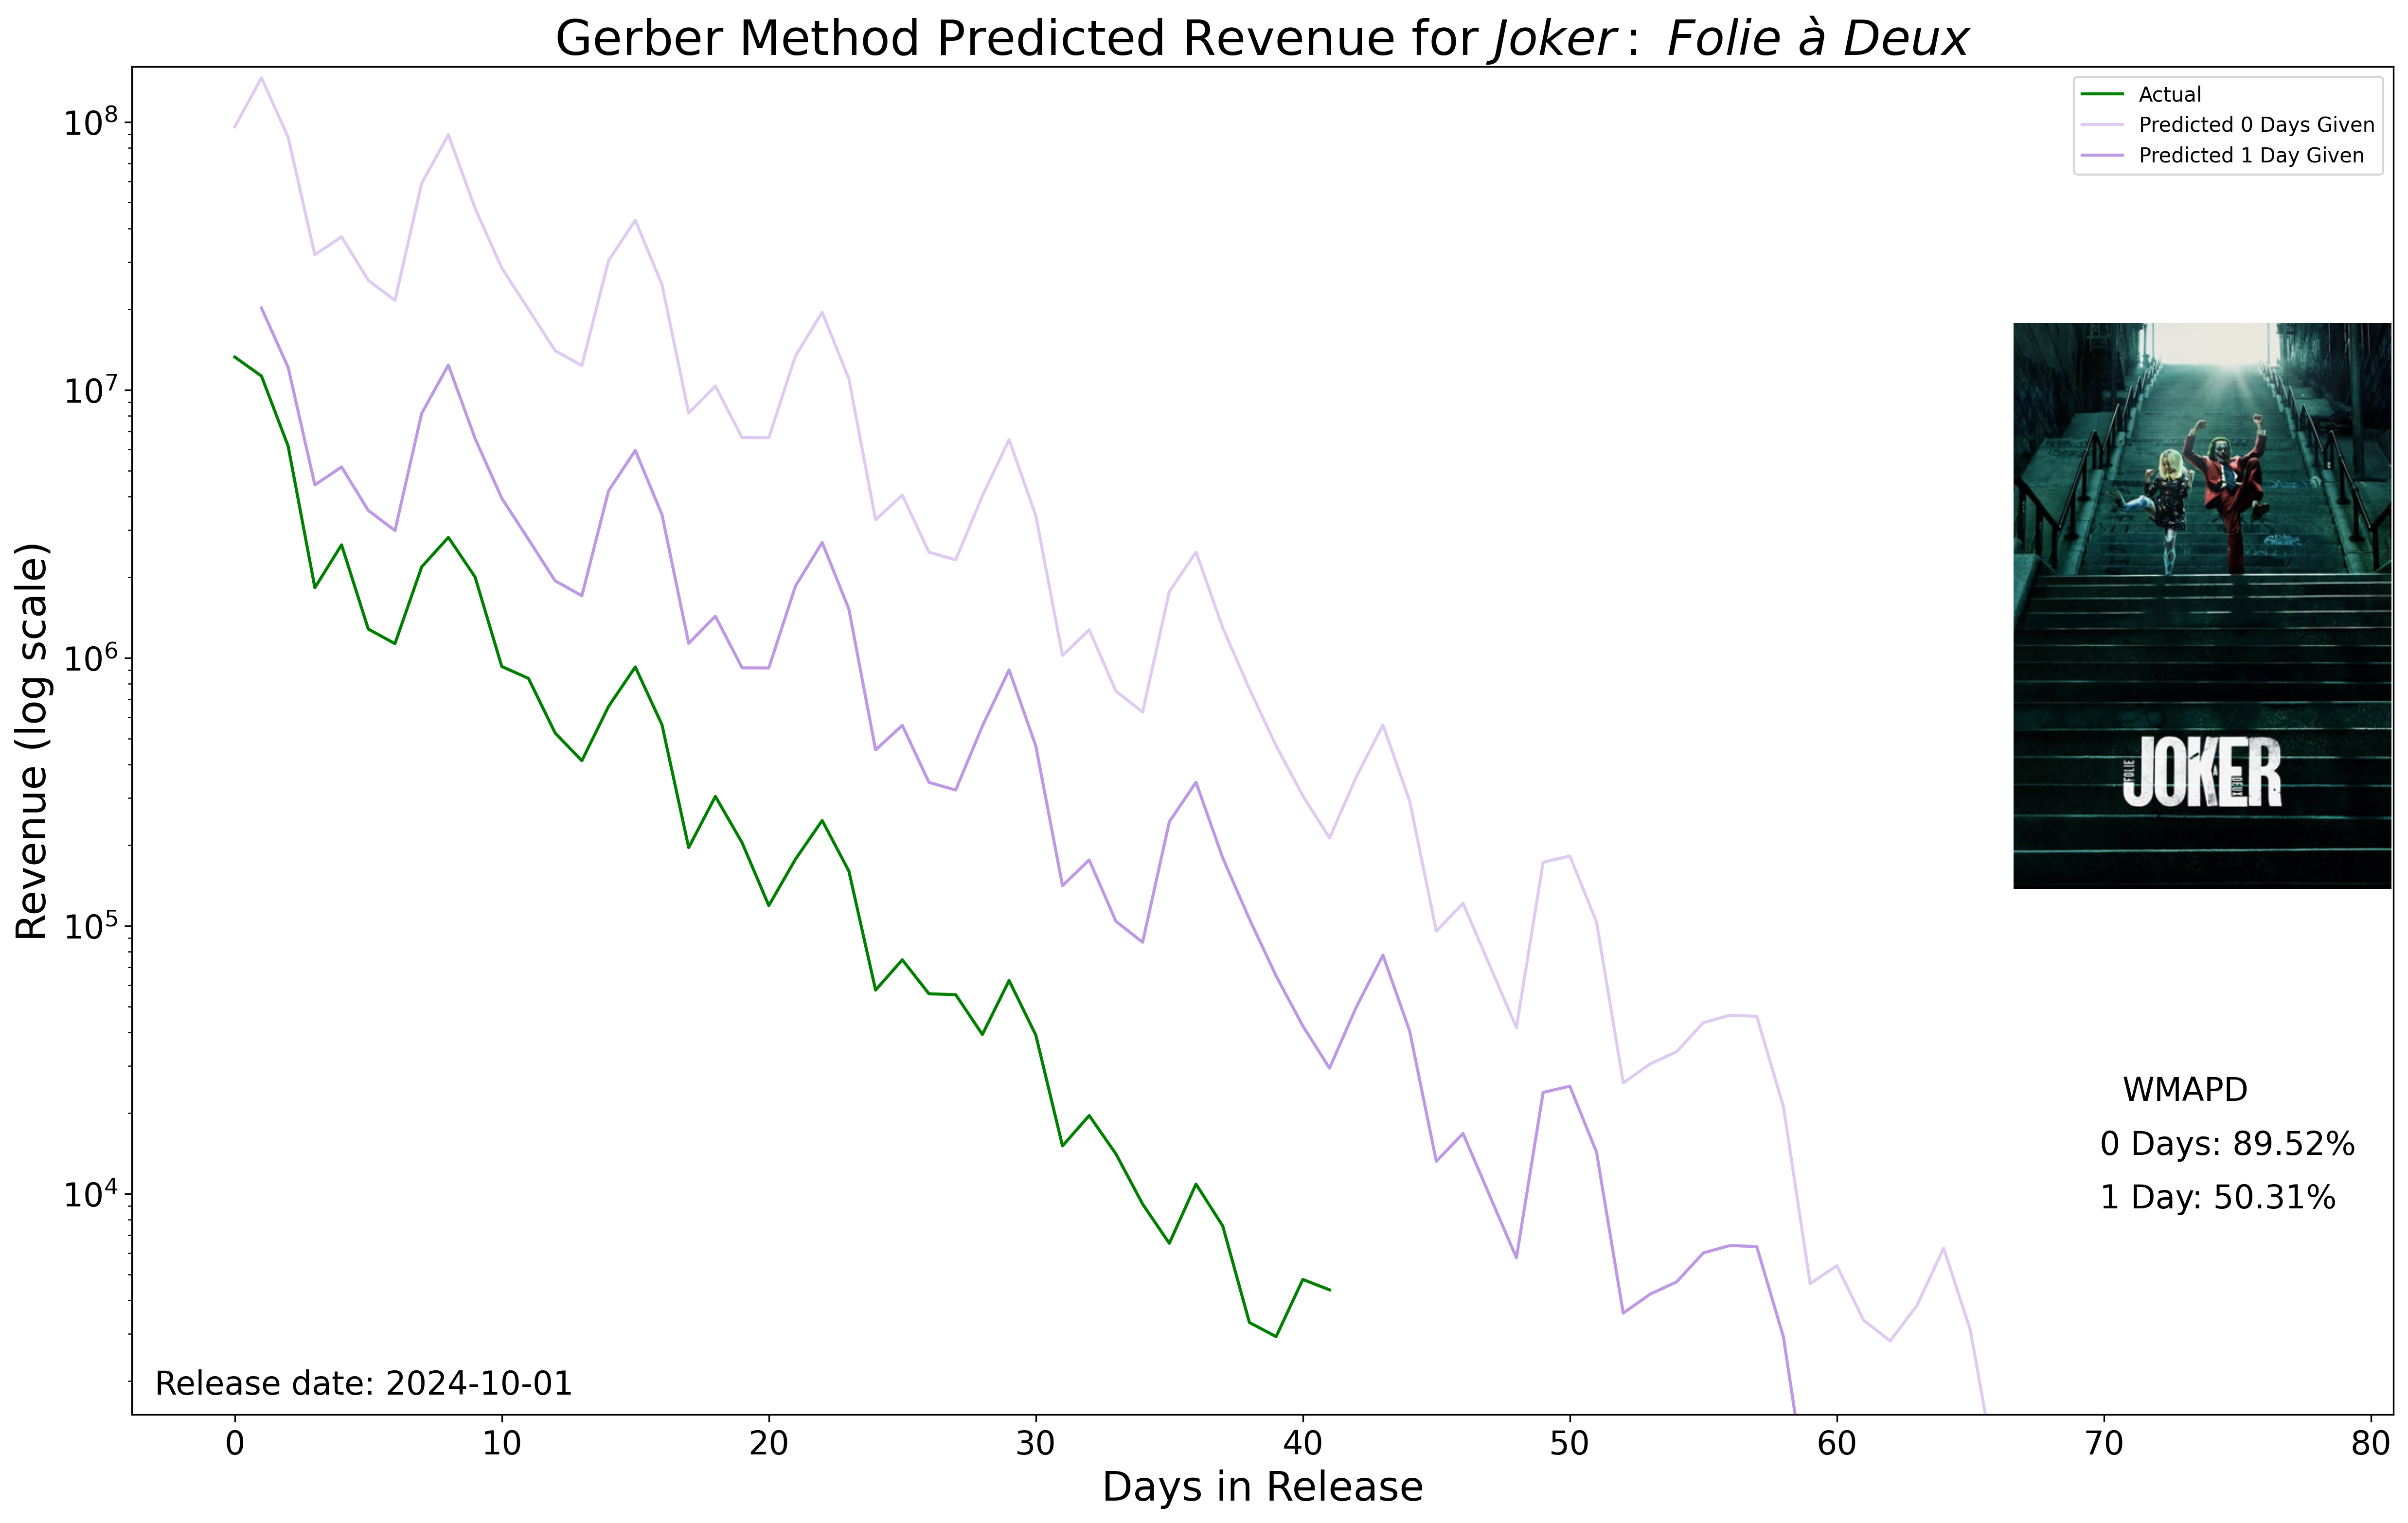
\includegraphics[width=0.95\textwidth]{../shared/images/pred/Joker: Folie à Deux_multiple_2.png}
  \end{figure}
  \addtocounter{framenumber}{-1}
\end{frame}

\begin{frame}{Results Multiple: \cite{jokerFolie}}
  \begin{figure}
    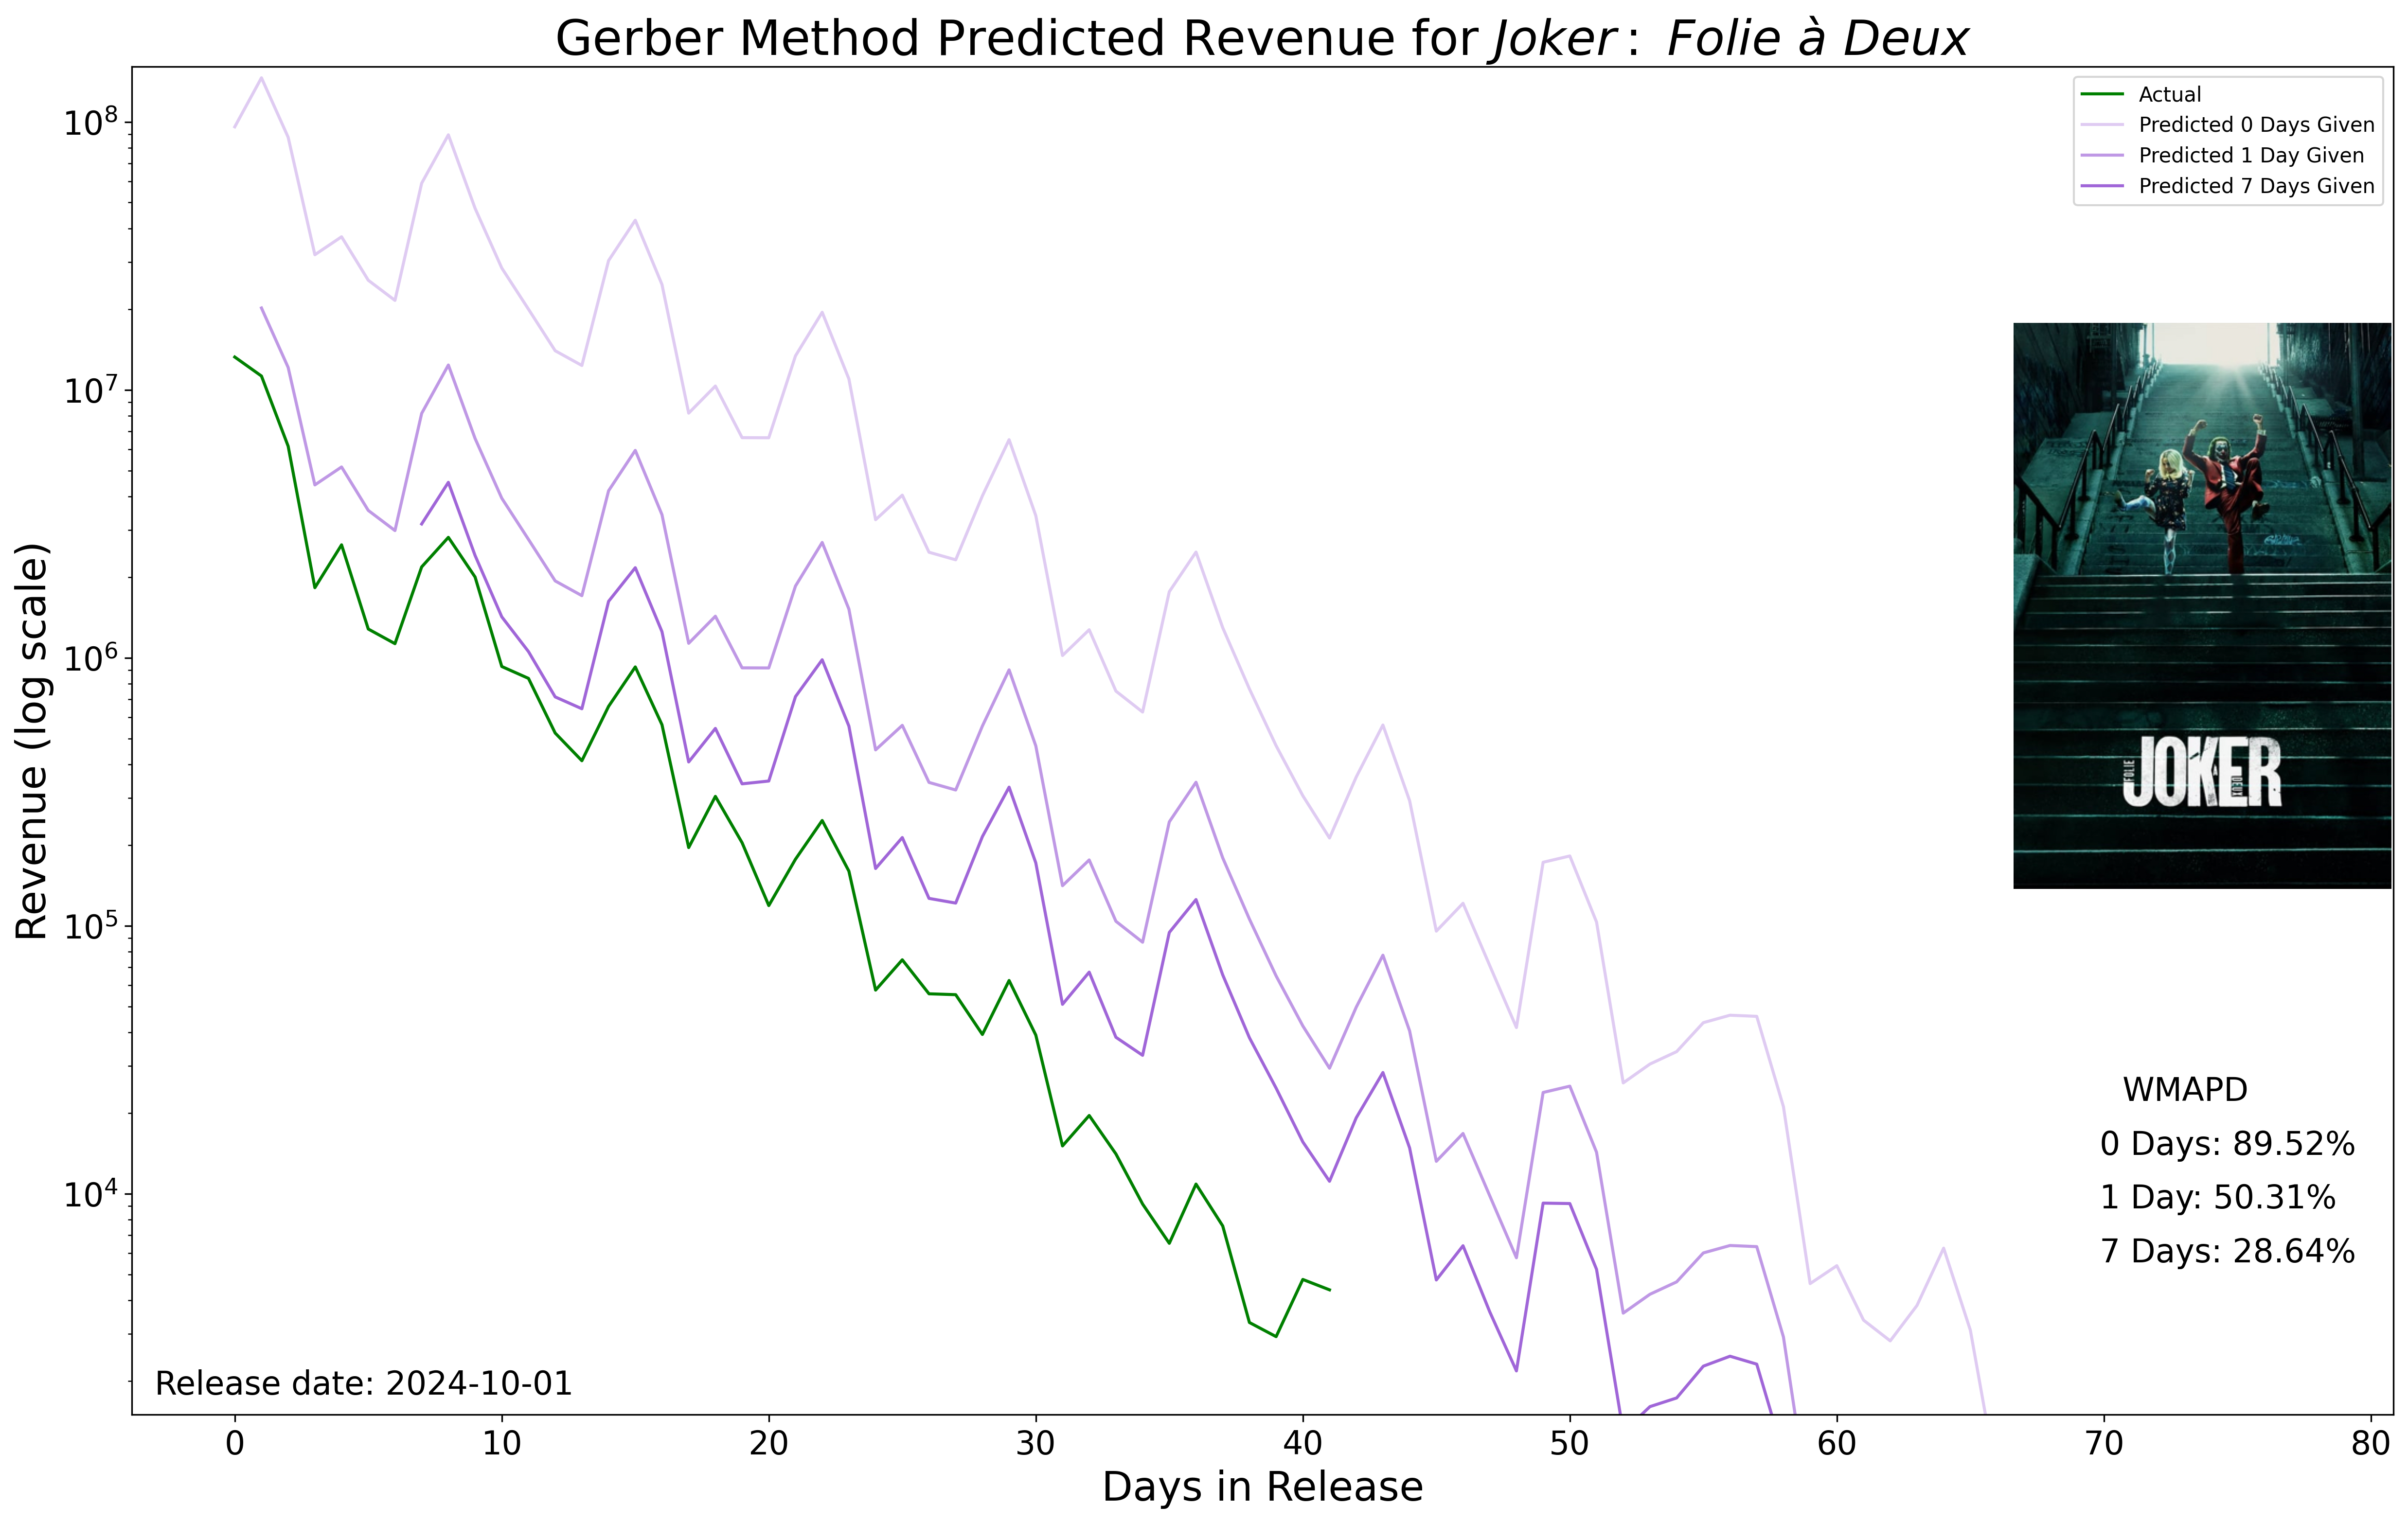
\includegraphics[width=0.95\textwidth]{../shared/images/pred/Joker: Folie à Deux_multiple_3.png}
  \end{figure}
  \addtocounter{framenumber}{-1}
\end{frame}

\begin{frame}{Results Multiple: \cite{jokerFolie}}
  \begin{figure}
    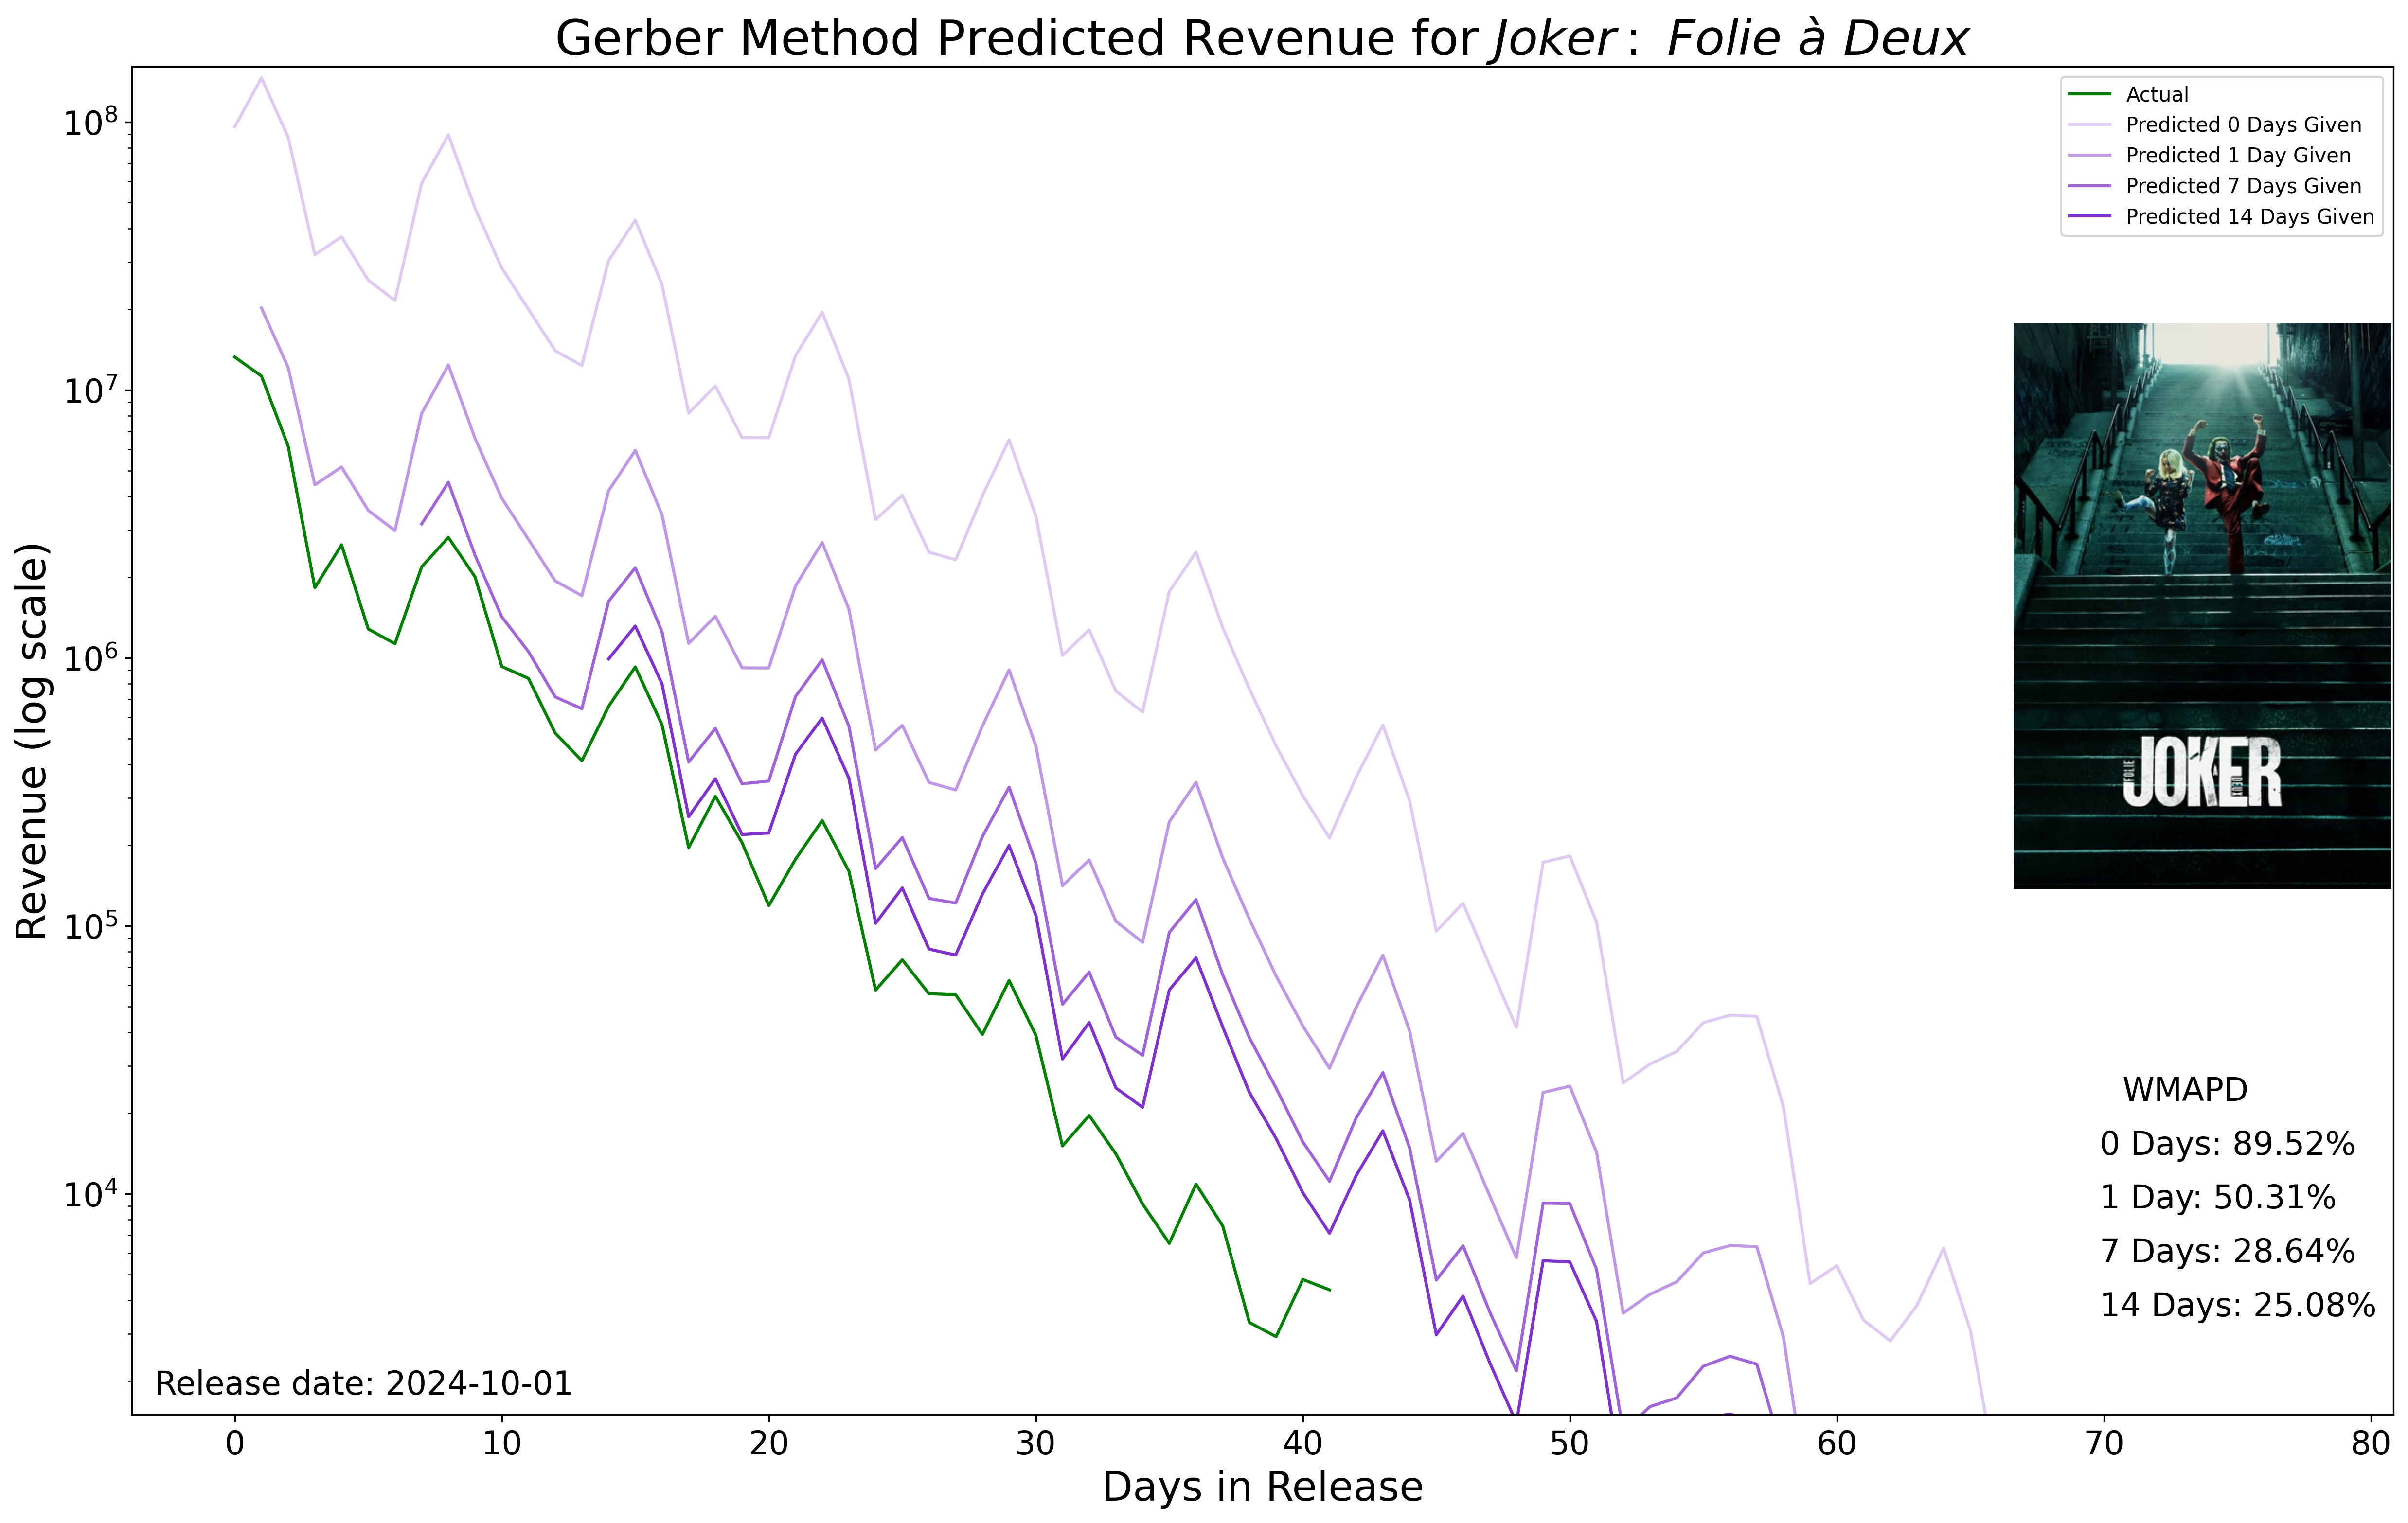
\includegraphics[width=0.95\textwidth]{../shared/images/pred/Joker: Folie à Deux_multiple_4.png}
  \end{figure}
  \addtocounter{framenumber}{-1}
\end{frame}

\begin{frame}{Results Multiple: \cite{conclave}}
  \begin{figure}
    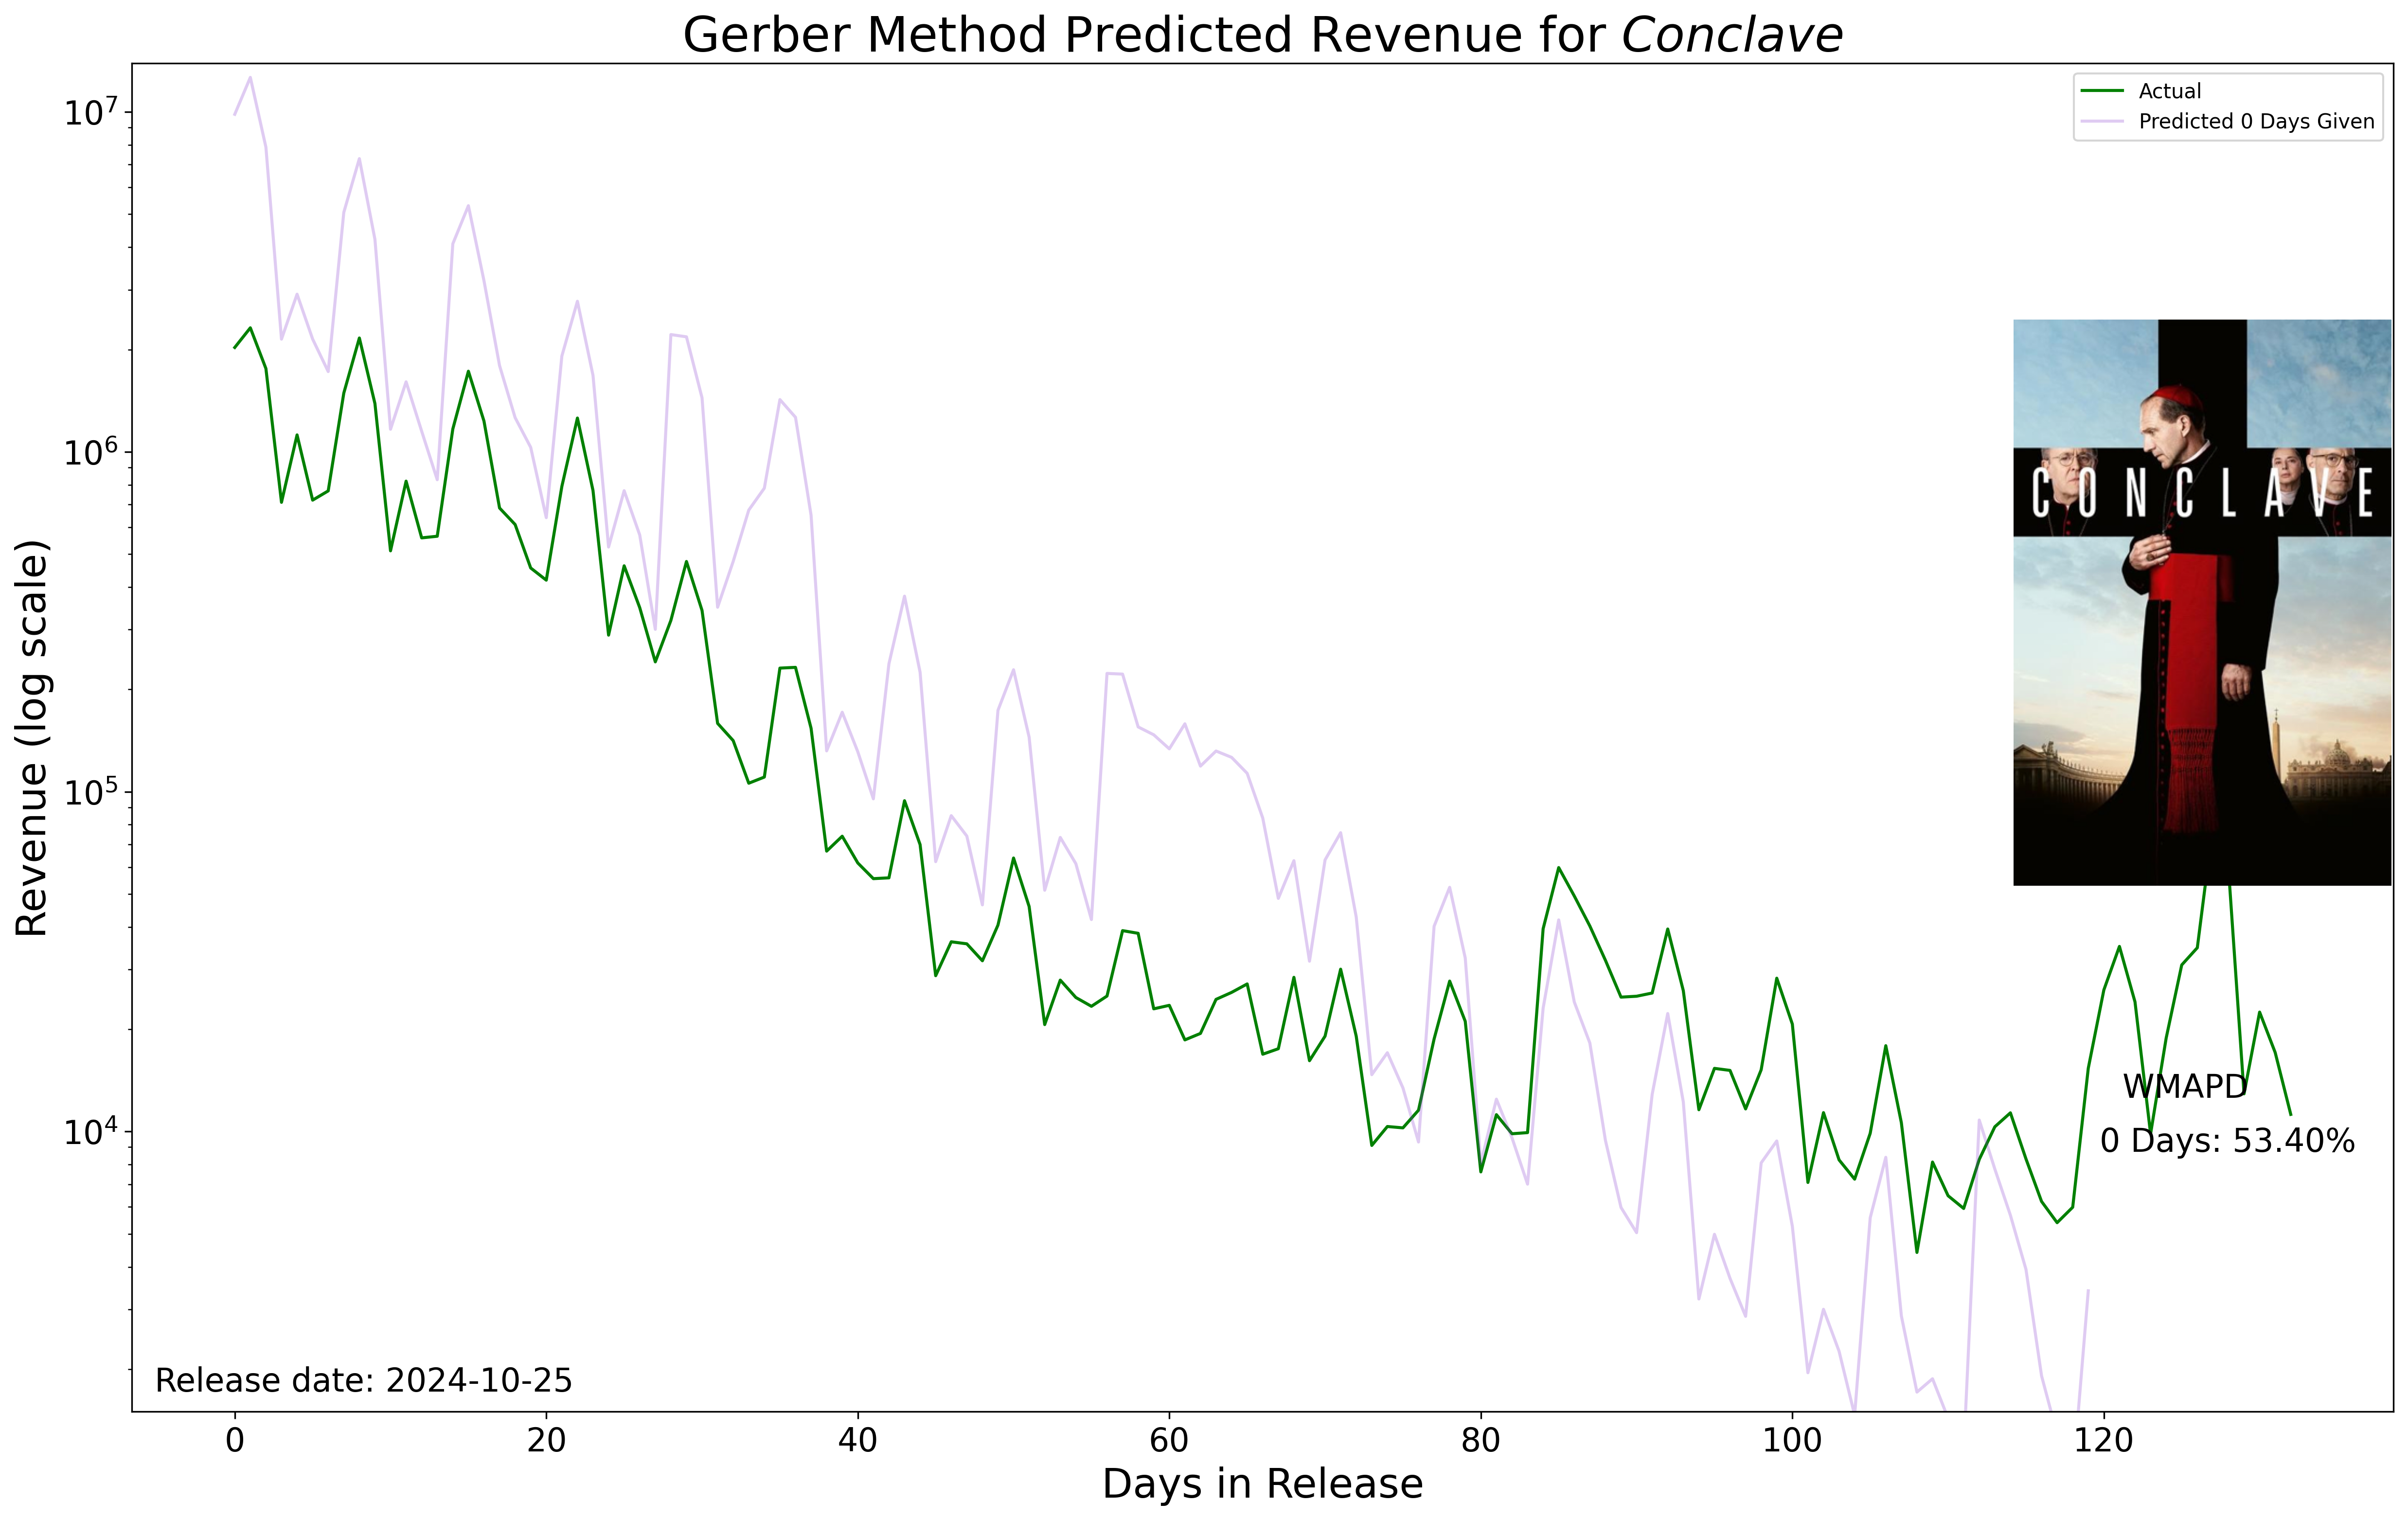
\includegraphics[width=0.95\textwidth]{../shared/images/pred/Conclave_multiple_1.png}
  \end{figure}
\end{frame}

\begin{frame}{Results Multiple: \cite{conclave}}
  \begin{figure}
    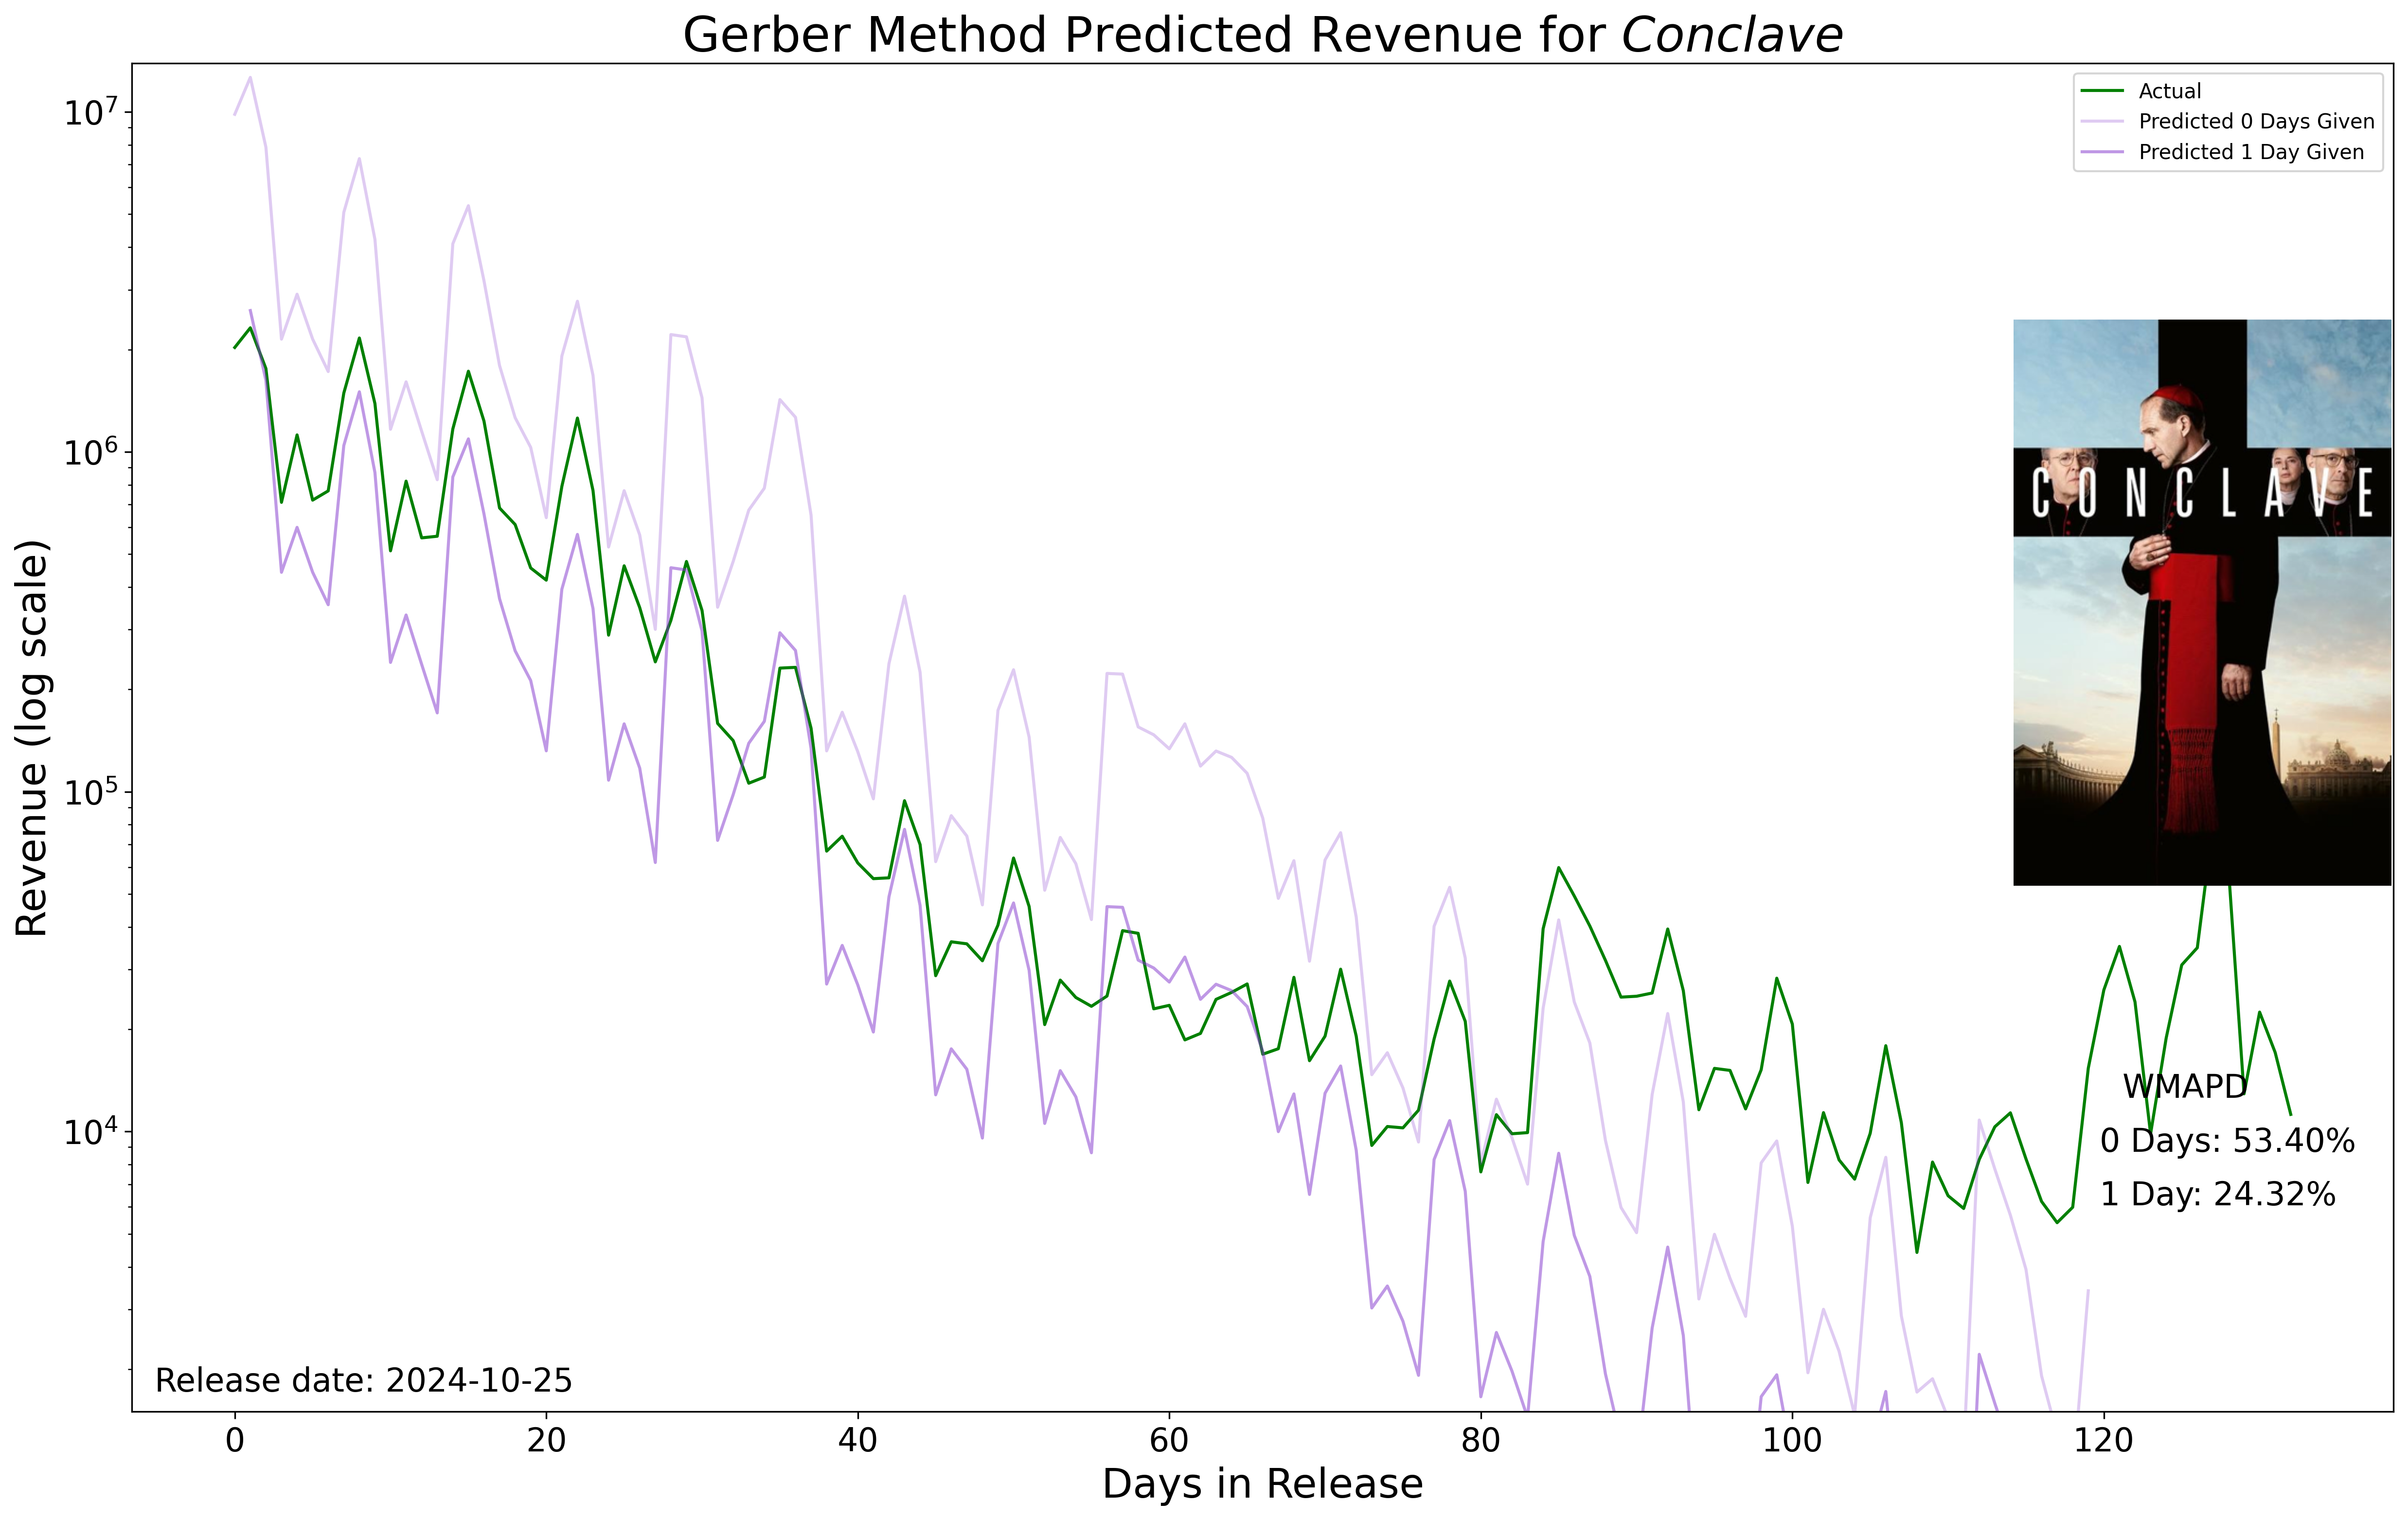
\includegraphics[width=0.95\textwidth]{../shared/images/pred/Conclave_multiple_2.png}
  \end{figure}
  \addtocounter{framenumber}{-1}
\end{frame}

\begin{frame}{Results Multiple: \cite{conclave}}
  \begin{figure}
    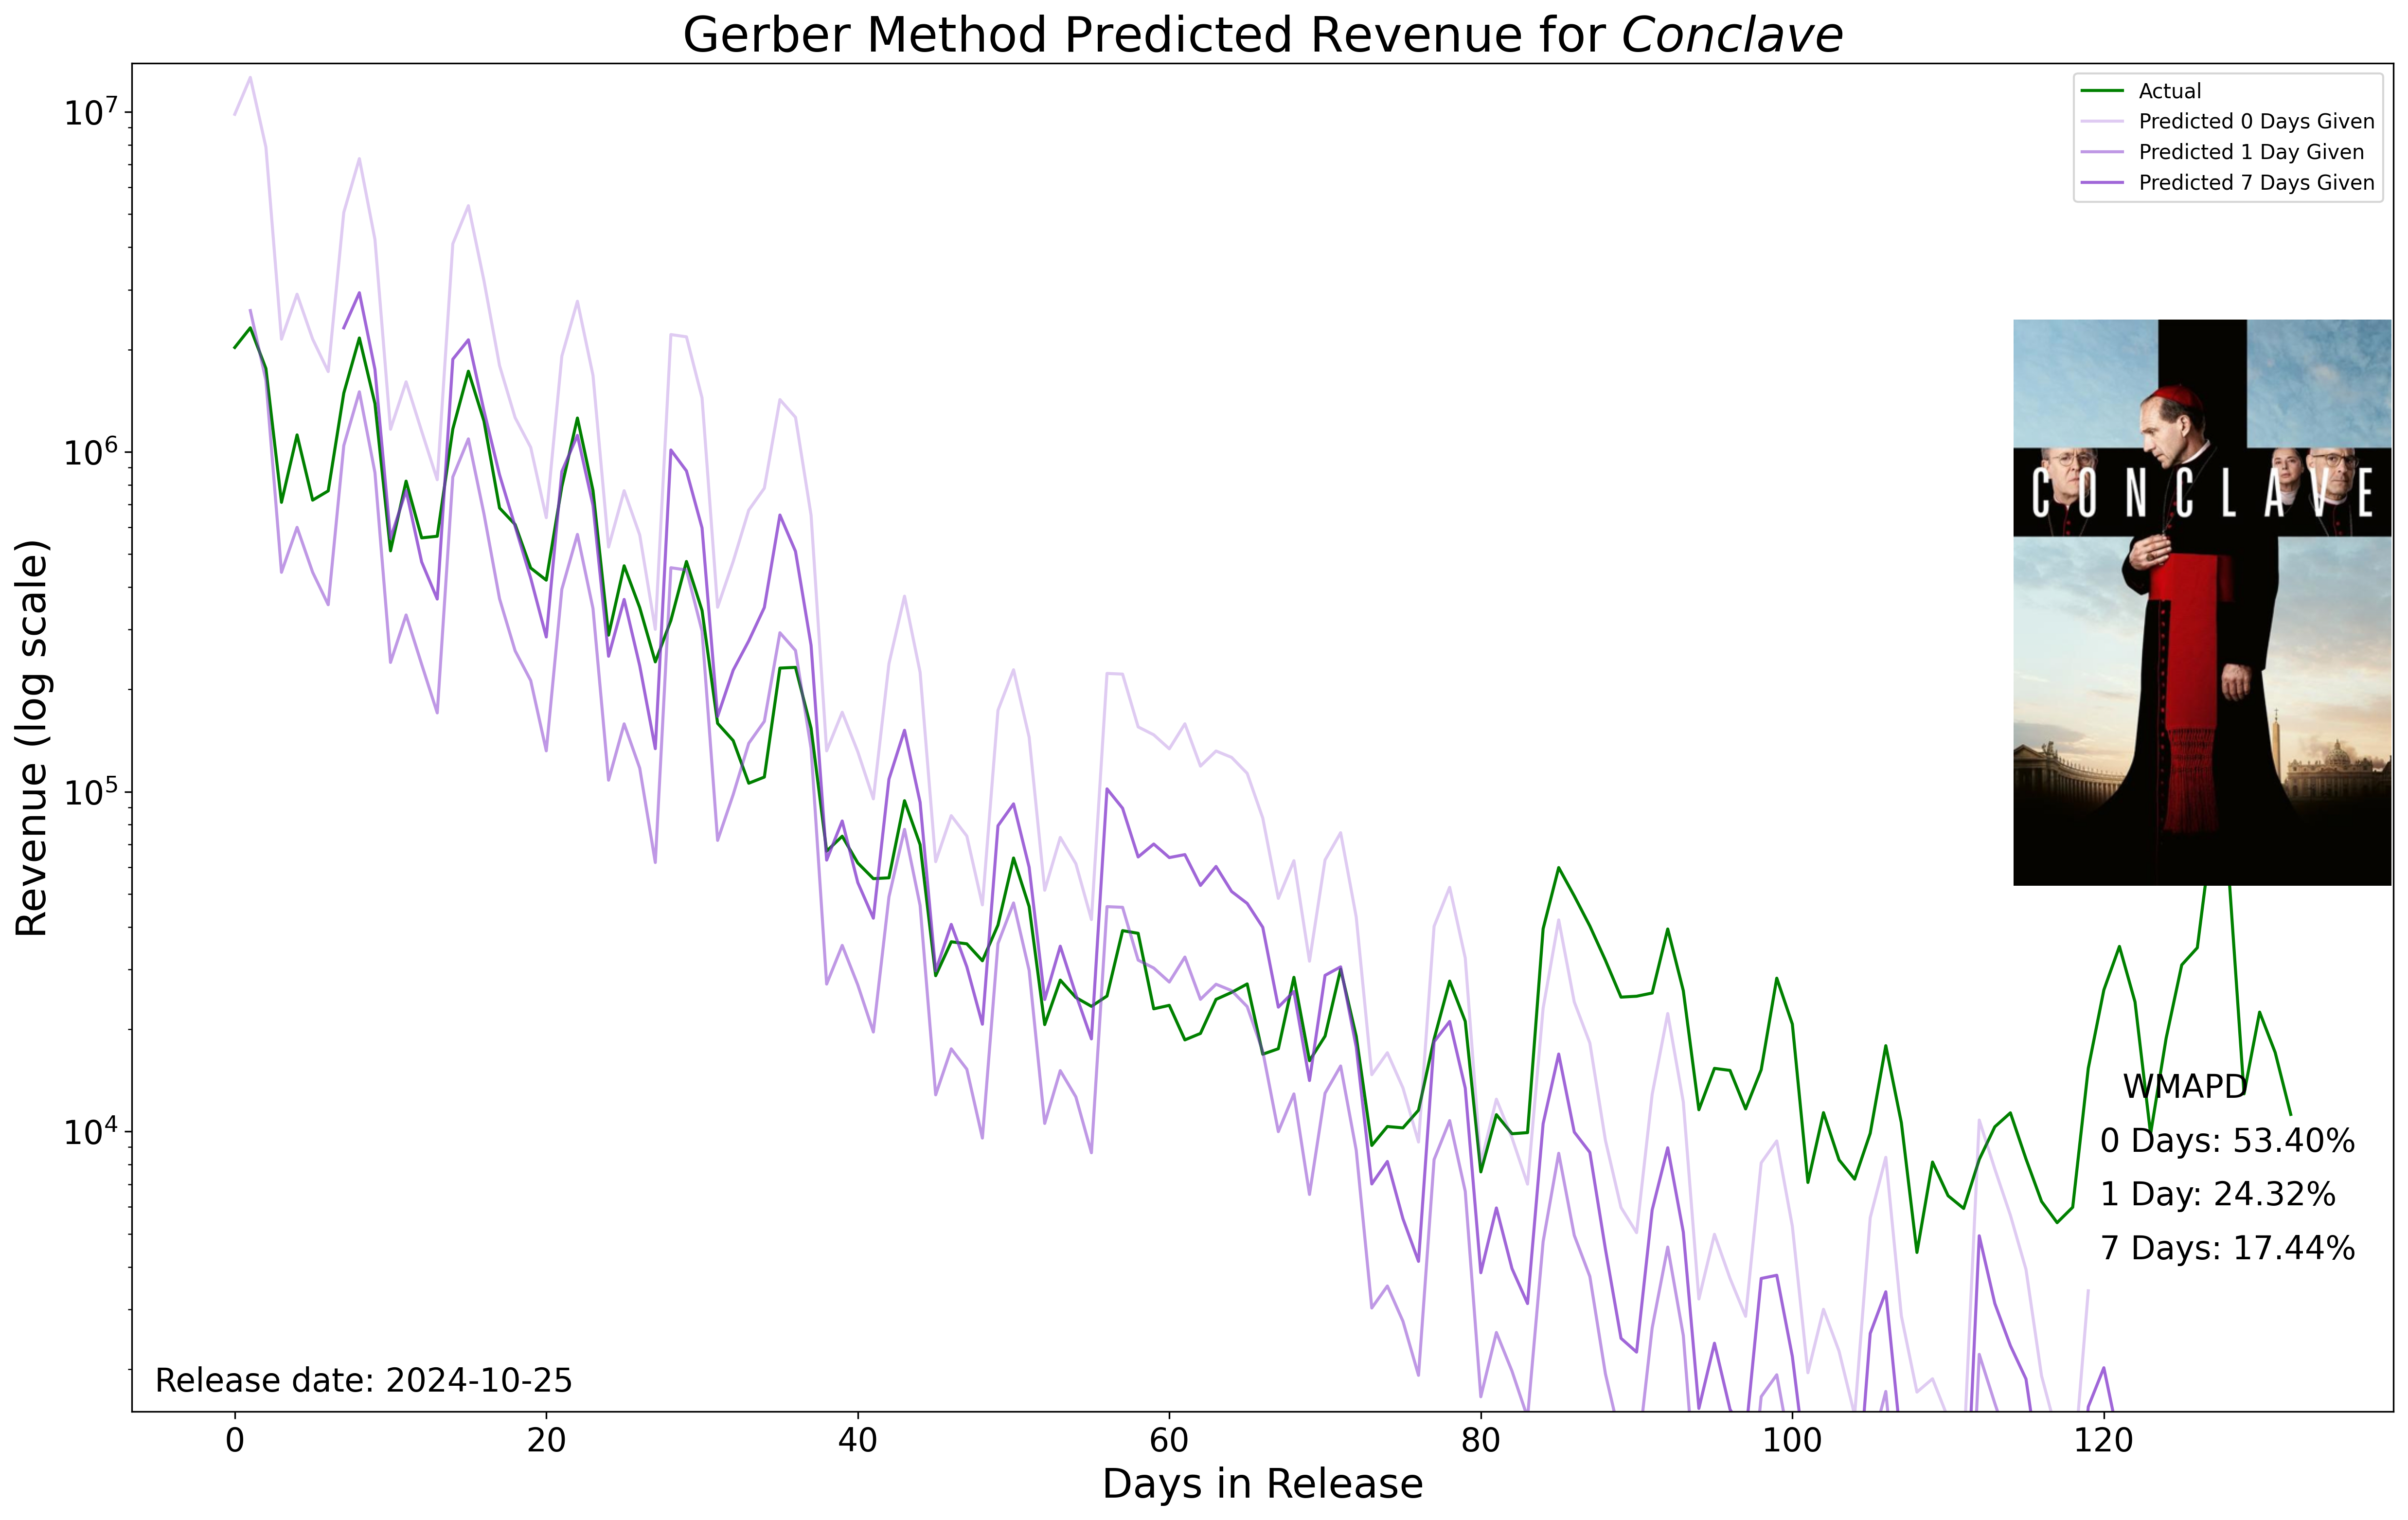
\includegraphics[width=0.95\textwidth]{../shared/images/pred/Conclave_multiple_3.png}
  \end{figure}
  \addtocounter{framenumber}{-1}
\end{frame}

\begin{frame}{Results Multiple: \cite{conclave}}
  \begin{figure}
    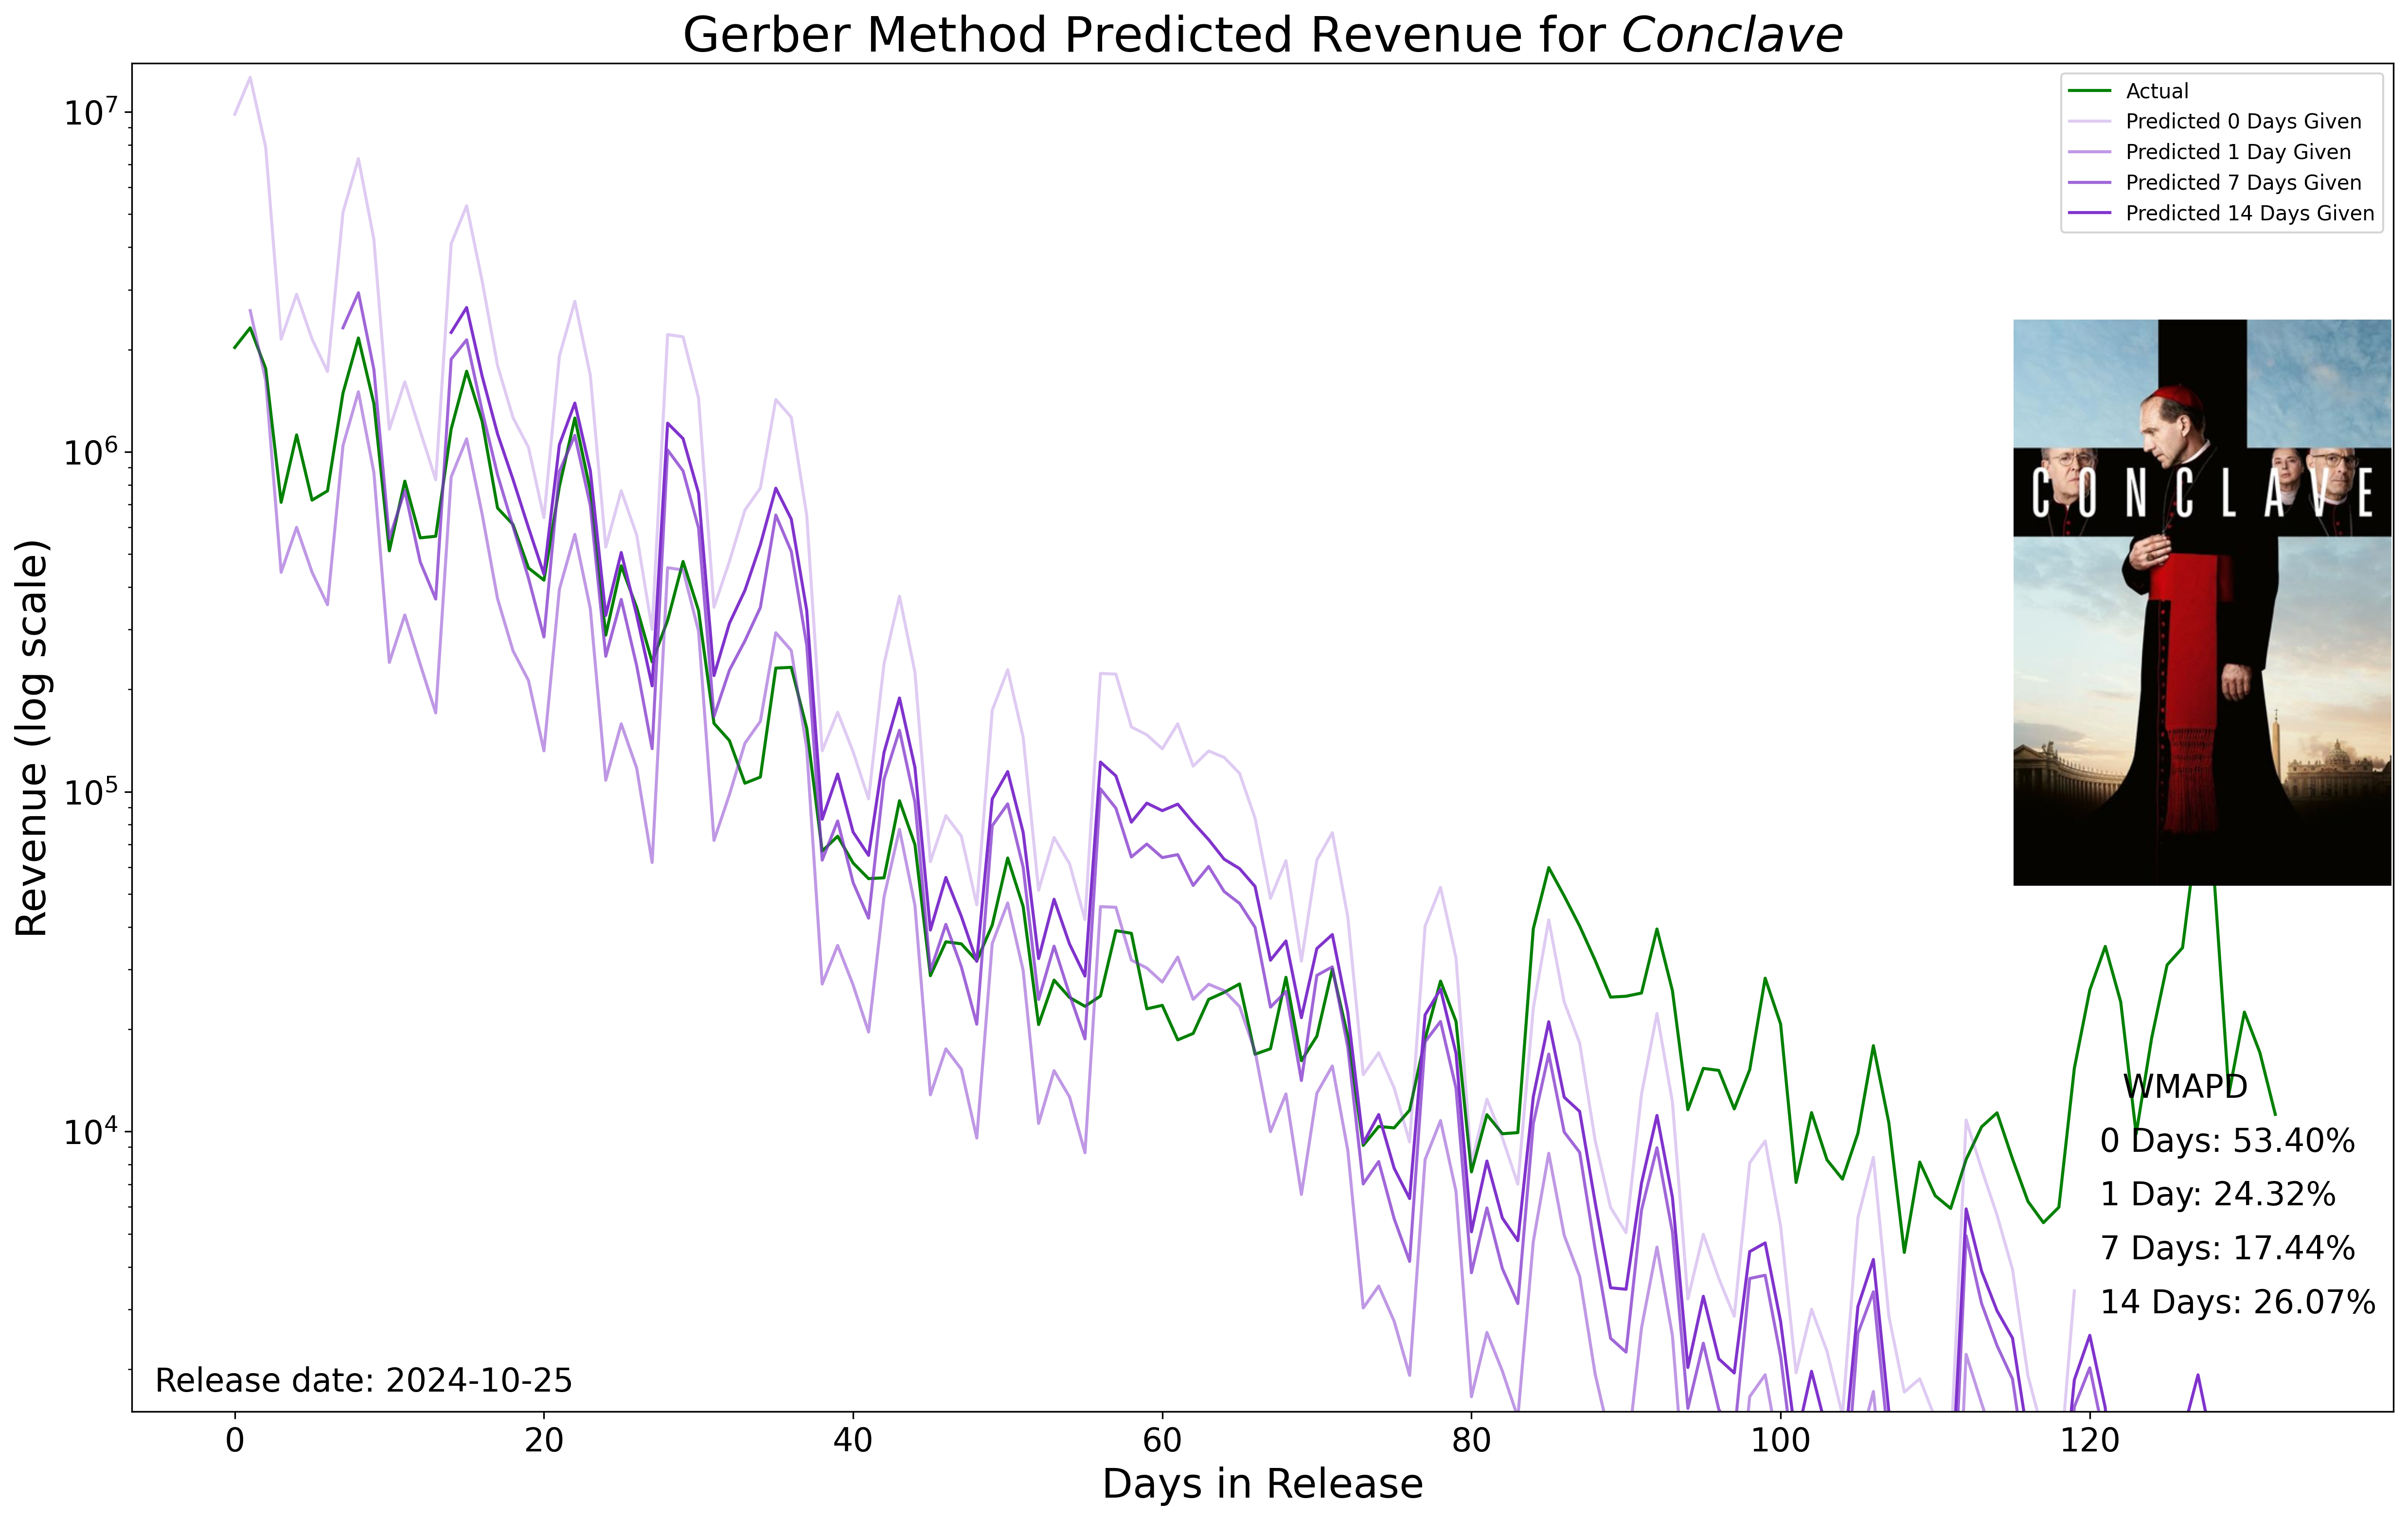
\includegraphics[width=0.95\textwidth]{../shared/images/pred/Conclave_multiple_4.png}
  \end{figure}
  \addtocounter{framenumber}{-1}
\end{frame}

\begin{frame}{Results Multiple: \cite{insideOut2}}
  \begin{figure}
    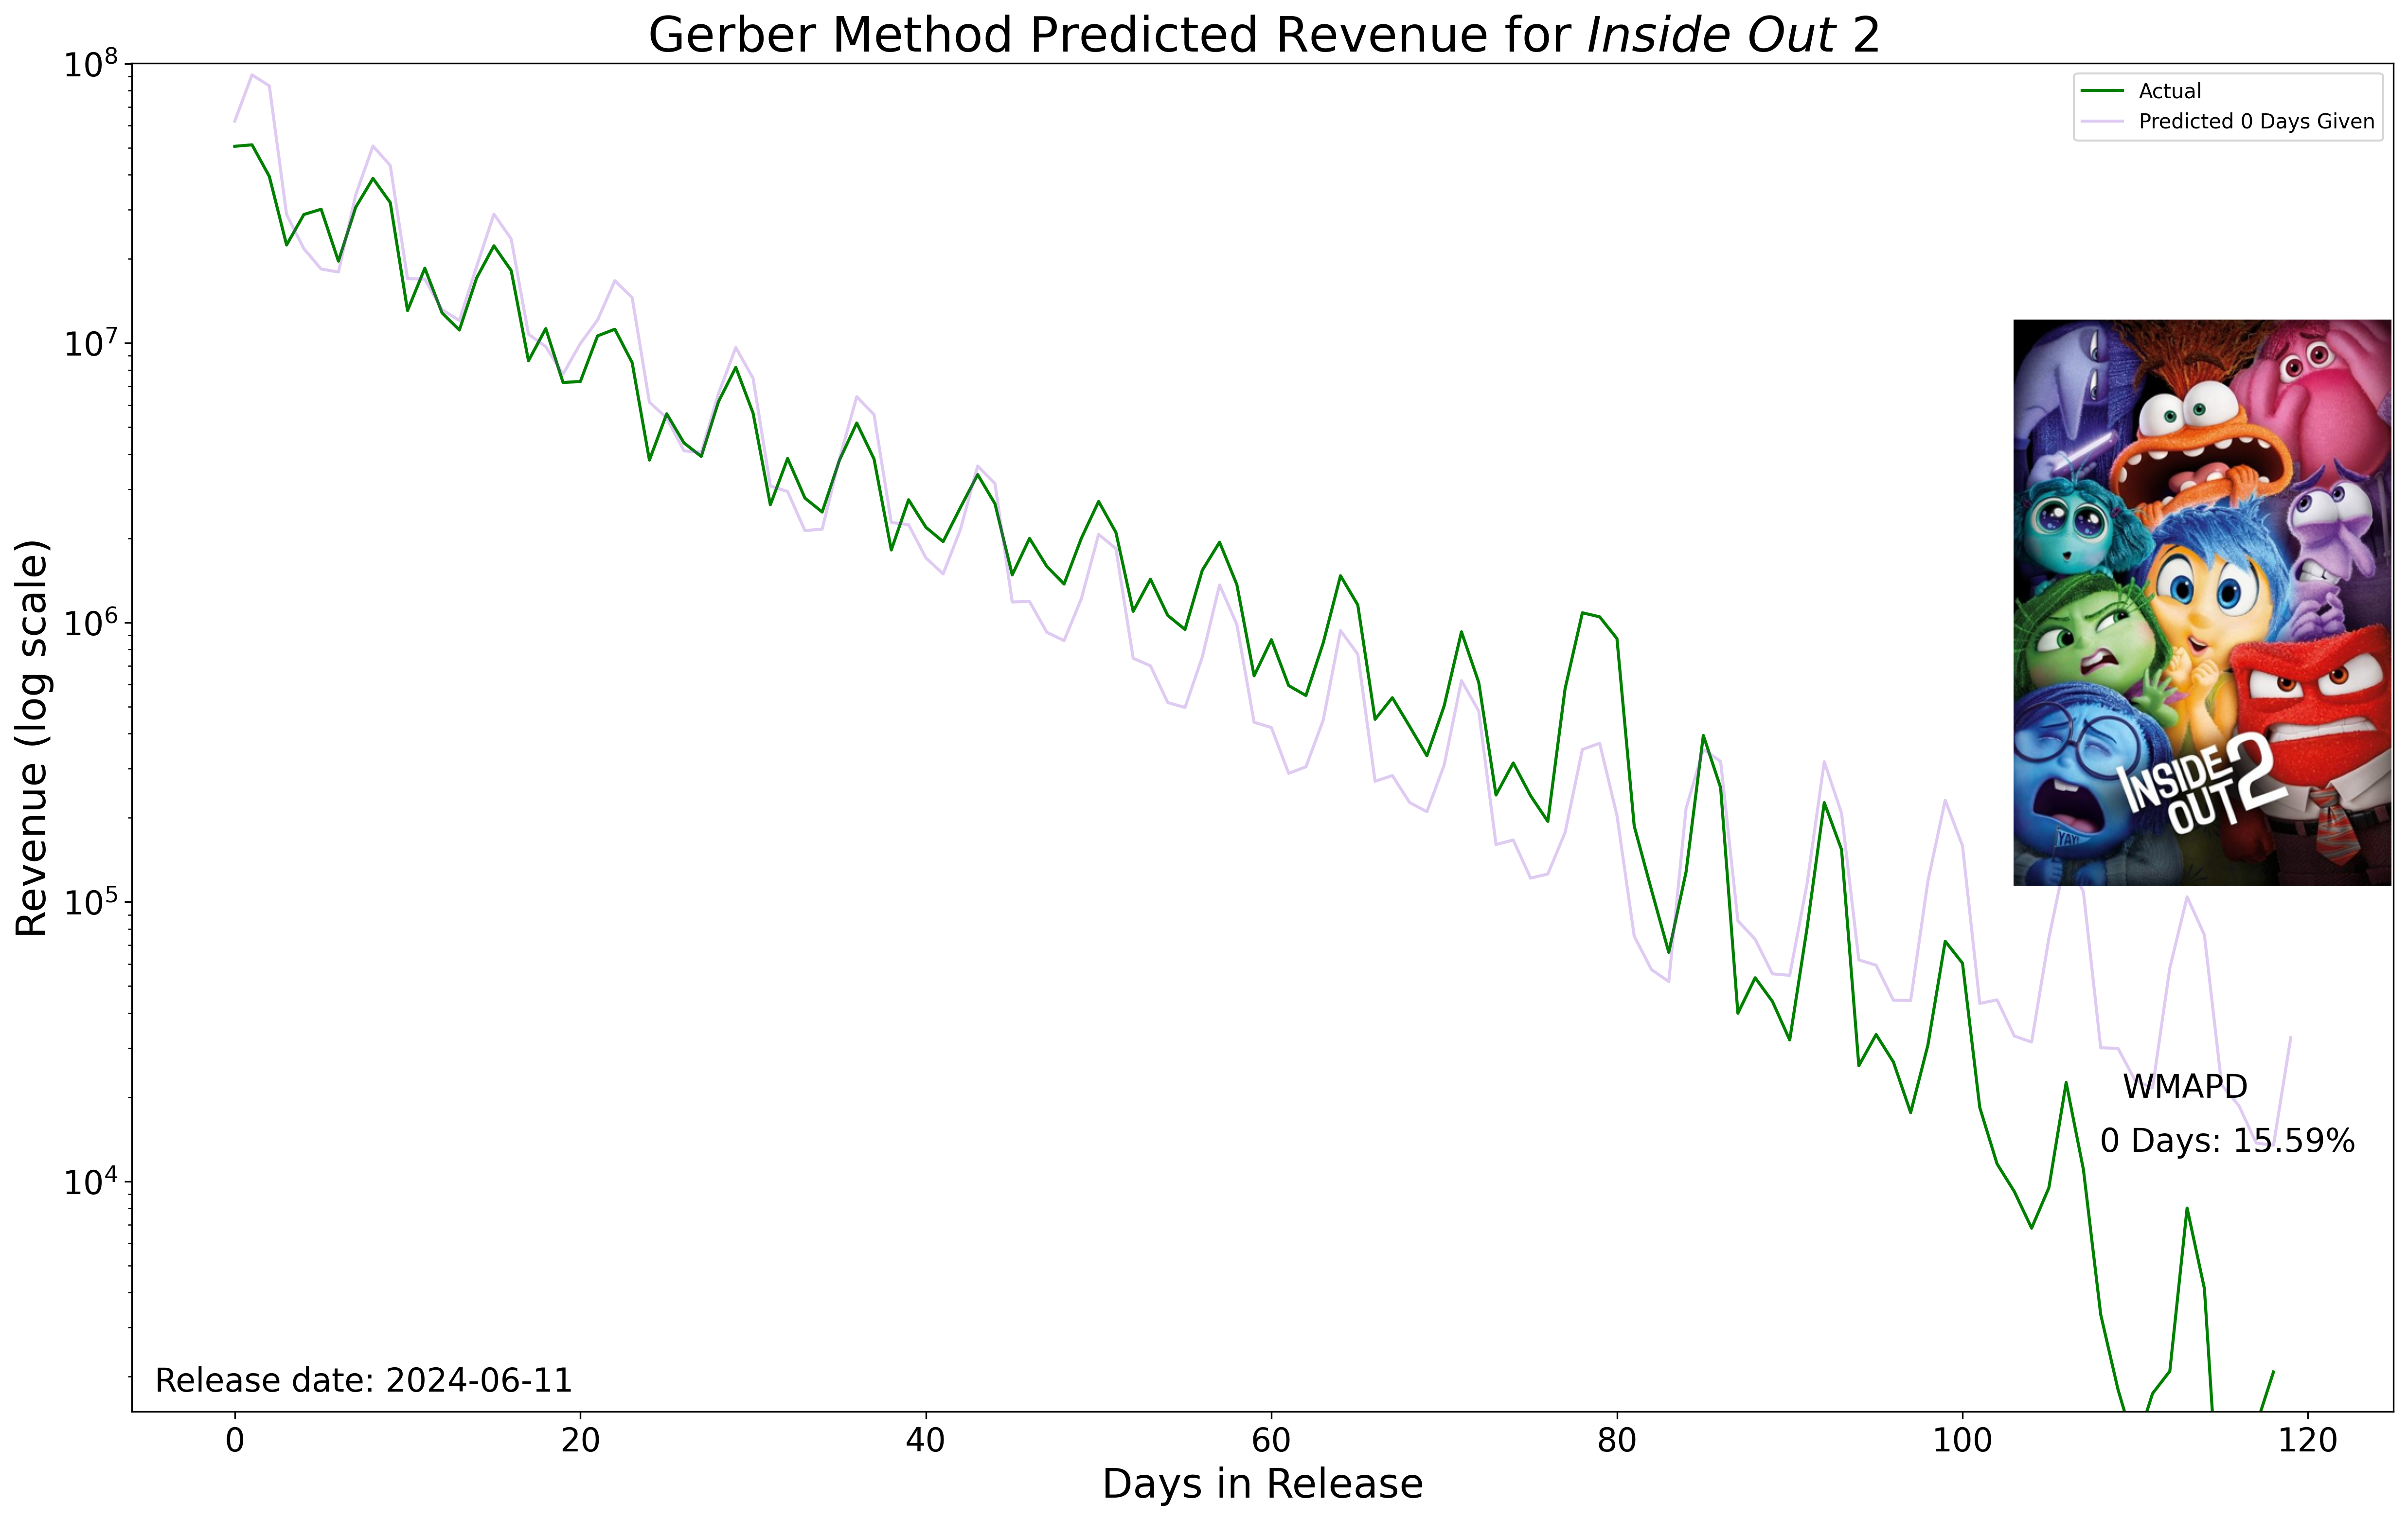
\includegraphics[width=0.95\textwidth]{../shared/images/pred/Inside Out 2_multiple_1.png}
  \end{figure}
\end{frame}

\begin{frame}{Results Multiple: \cite{insideOut2}}
  \begin{figure}
    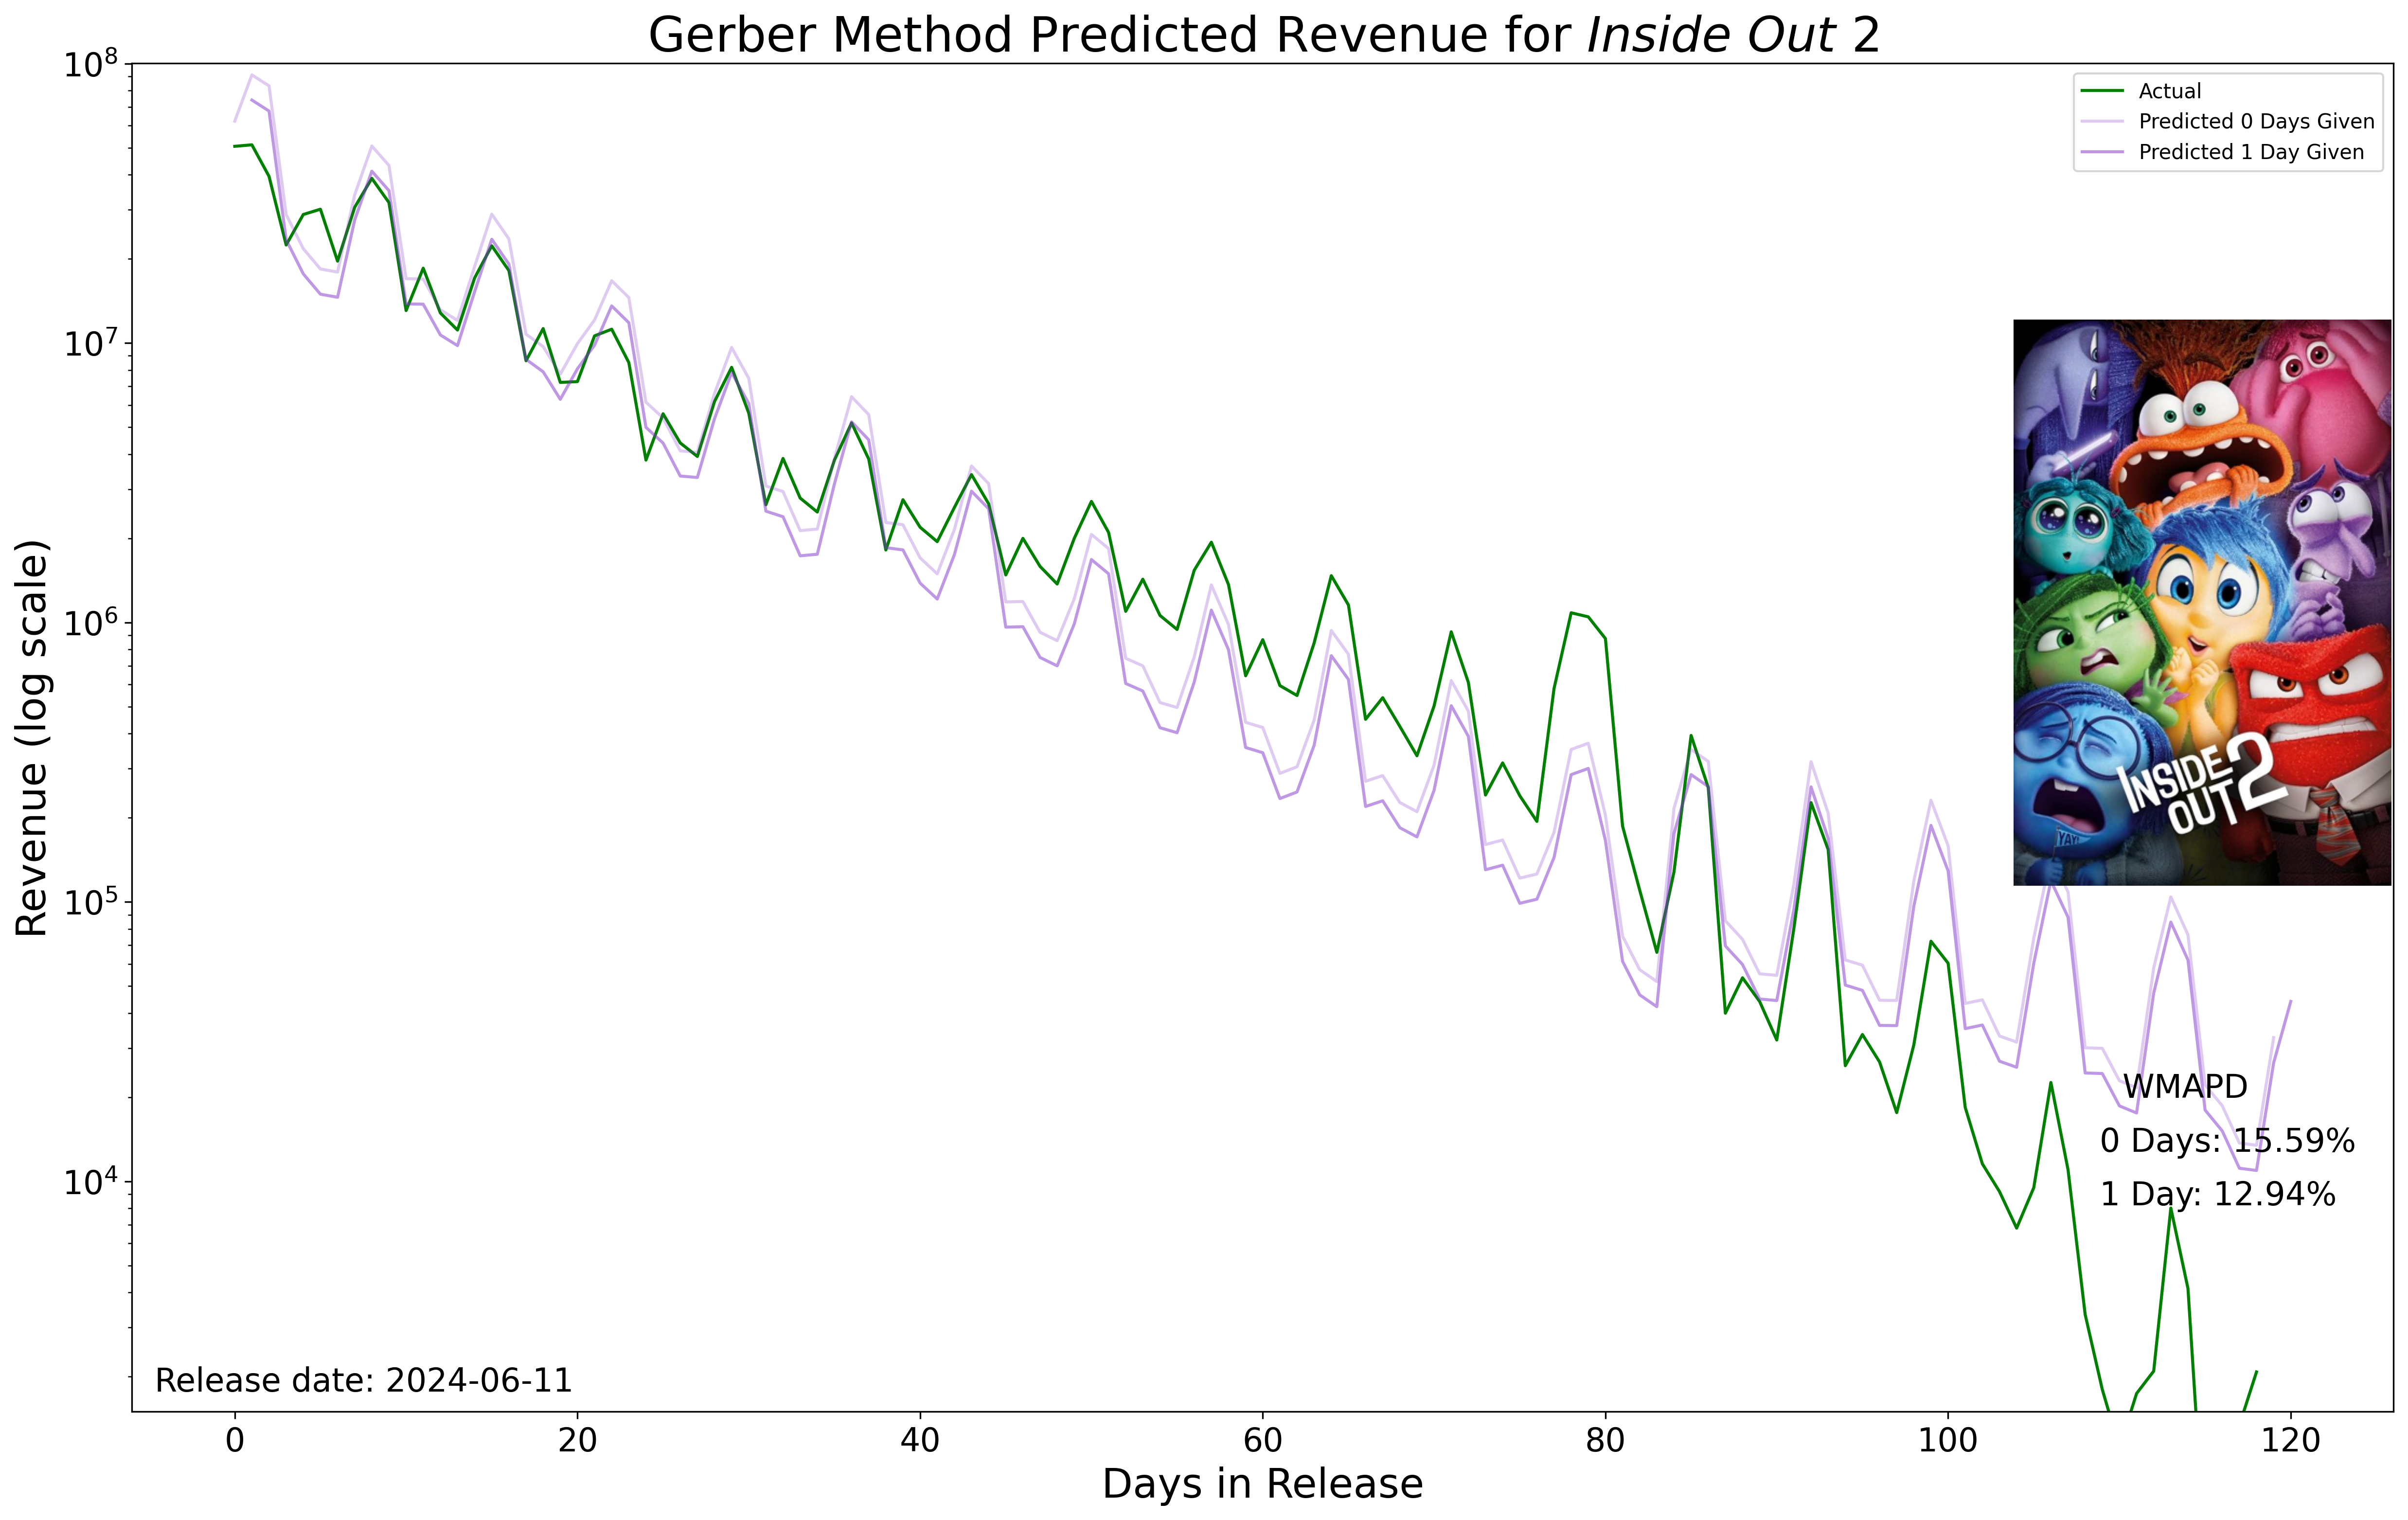
\includegraphics[width=0.95\textwidth]{../shared/images/pred/Inside Out 2_multiple_2.png}
  \end{figure}
  \addtocounter{framenumber}{-1}
\end{frame}

\begin{frame}{Results Multiple: \cite{insideOut2}}
  \begin{figure}
    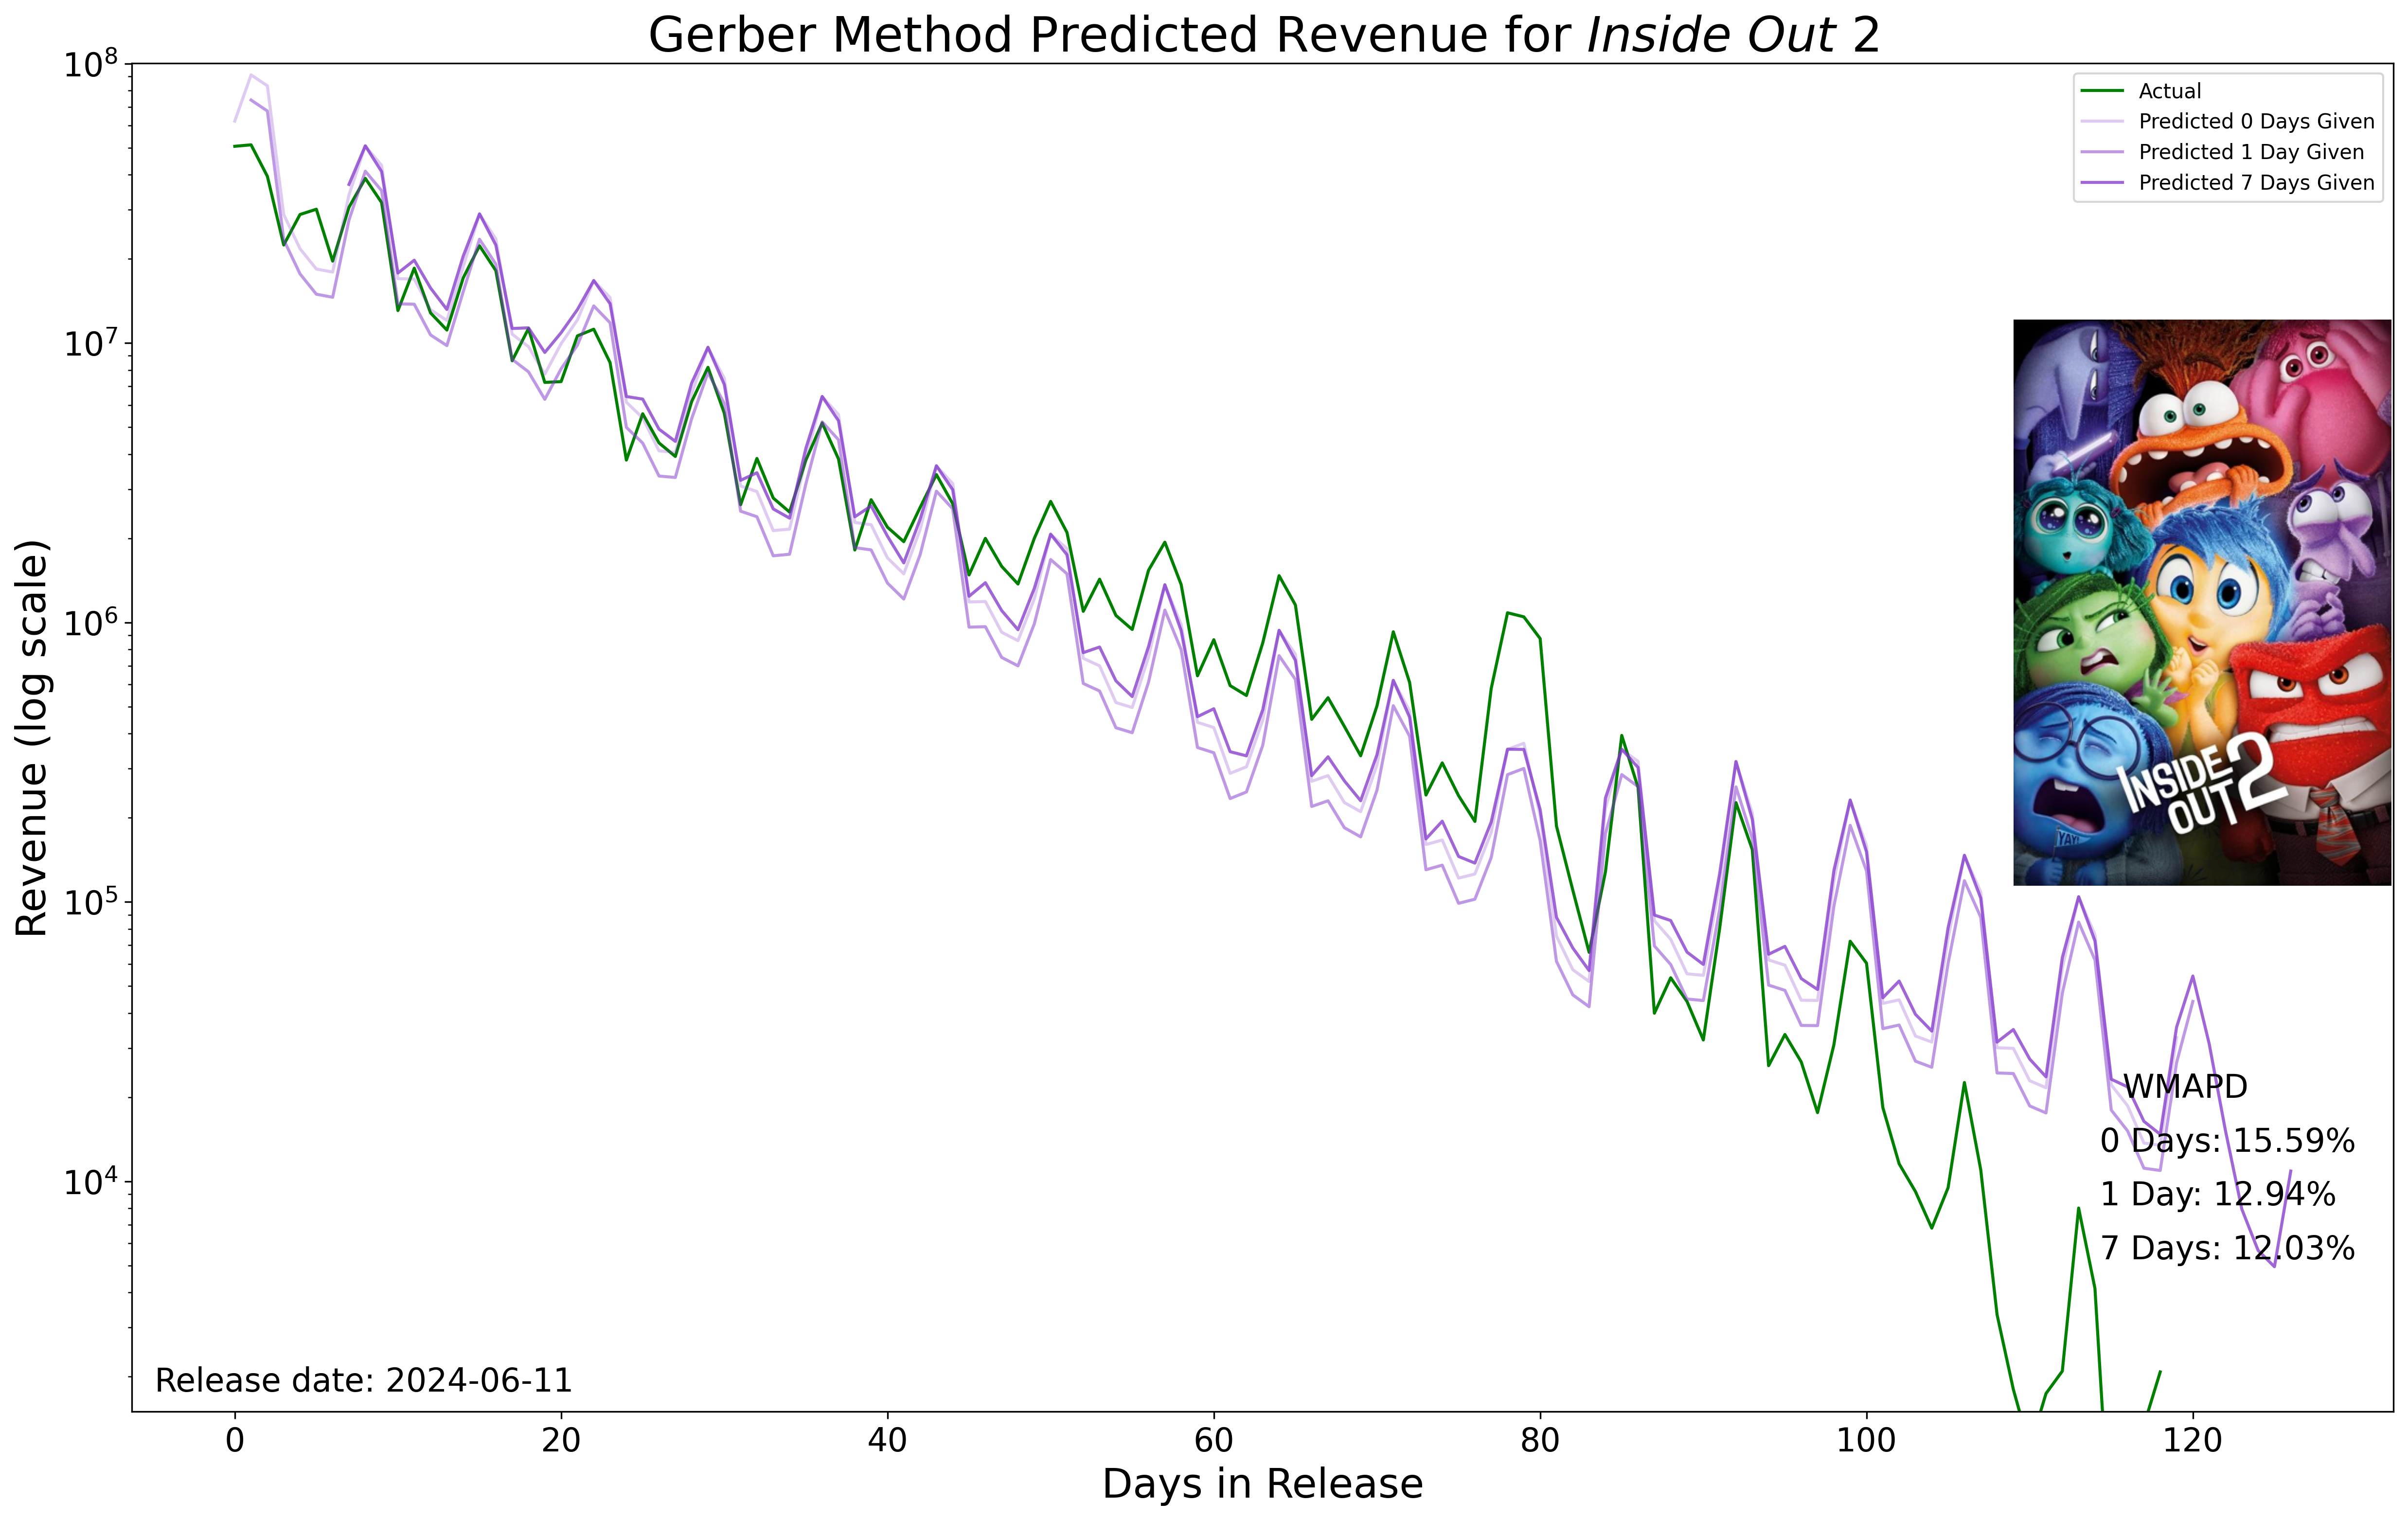
\includegraphics[width=0.95\textwidth]{../shared/images/pred/Inside Out 2_multiple_3.png}
  \end{figure}
  \addtocounter{framenumber}{-1}
\end{frame}

\begin{frame}{Results Multiple: \cite{insideOut2}}
  \begin{figure}
    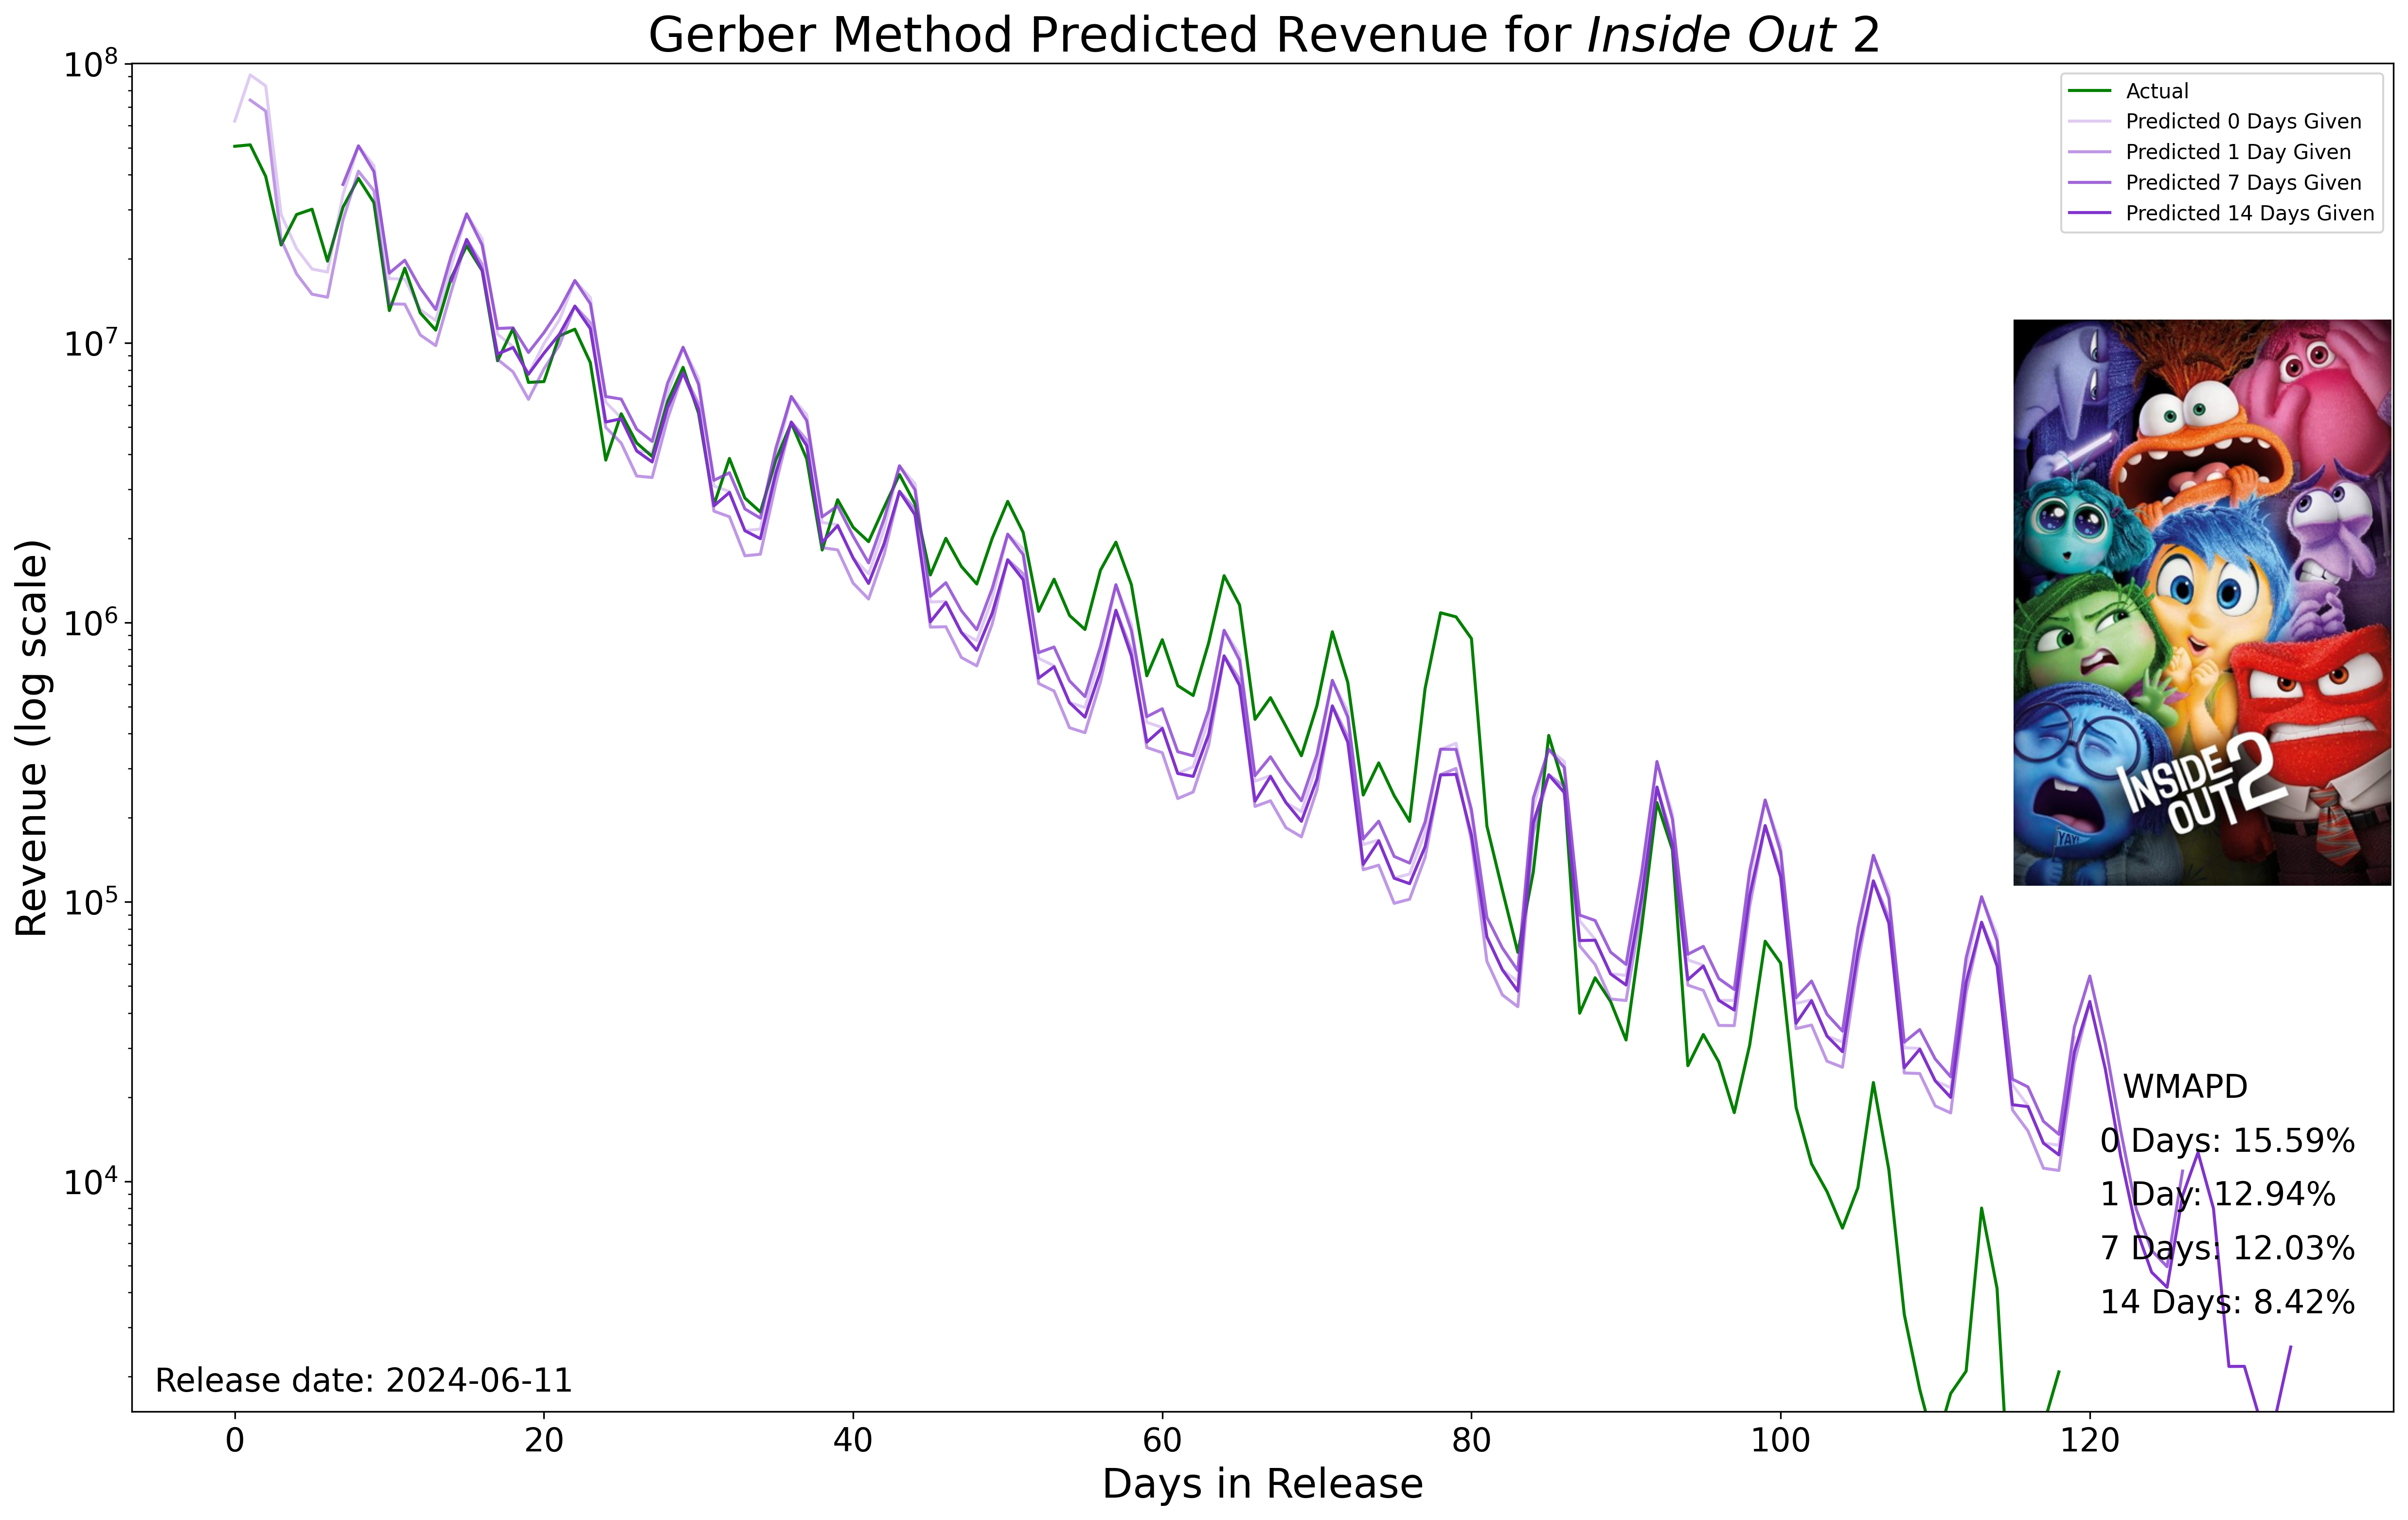
\includegraphics[width=0.95\textwidth]{../shared/images/pred/Inside Out 2_multiple_4.png}
  \end{figure}
  \addtocounter{framenumber}{-1}
  % Inside Out 2 re-released around labor day weekend to try to make it to the top 10 all time domestic first-run grosses and pass Jurassic World
\end{frame}

\begin{frame}{Metrics Box Plot}
  \begin{figure}
    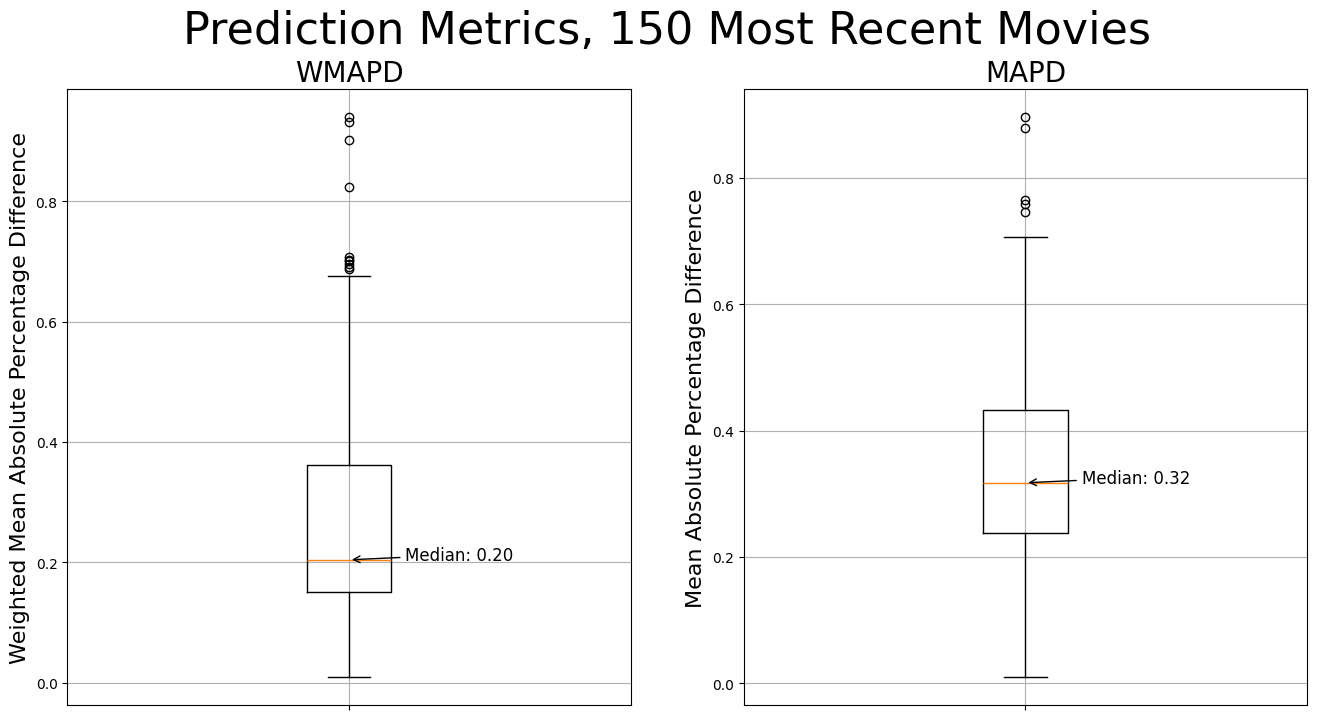
\includegraphics[width=0.92\textwidth]{../shared/images/results150small.png}
  \end{figure}
\end{frame}

\section{Conclusion}

\begin{frame}{Conclusion}
  Multipliers are an effective way of predicting daily box office
  \begin{itemize}
    \item Automated algorithms like KNN can find similar movies
    \item The model is able to predict box office for all types of releases
    \item Utilized appropriate adjustments to improve predictions
    \item This type of complete daily time series has never been done before
  \end{itemize}
  Next steps are to build a web app to provide predictions to interested parties

  \begin{figure}
    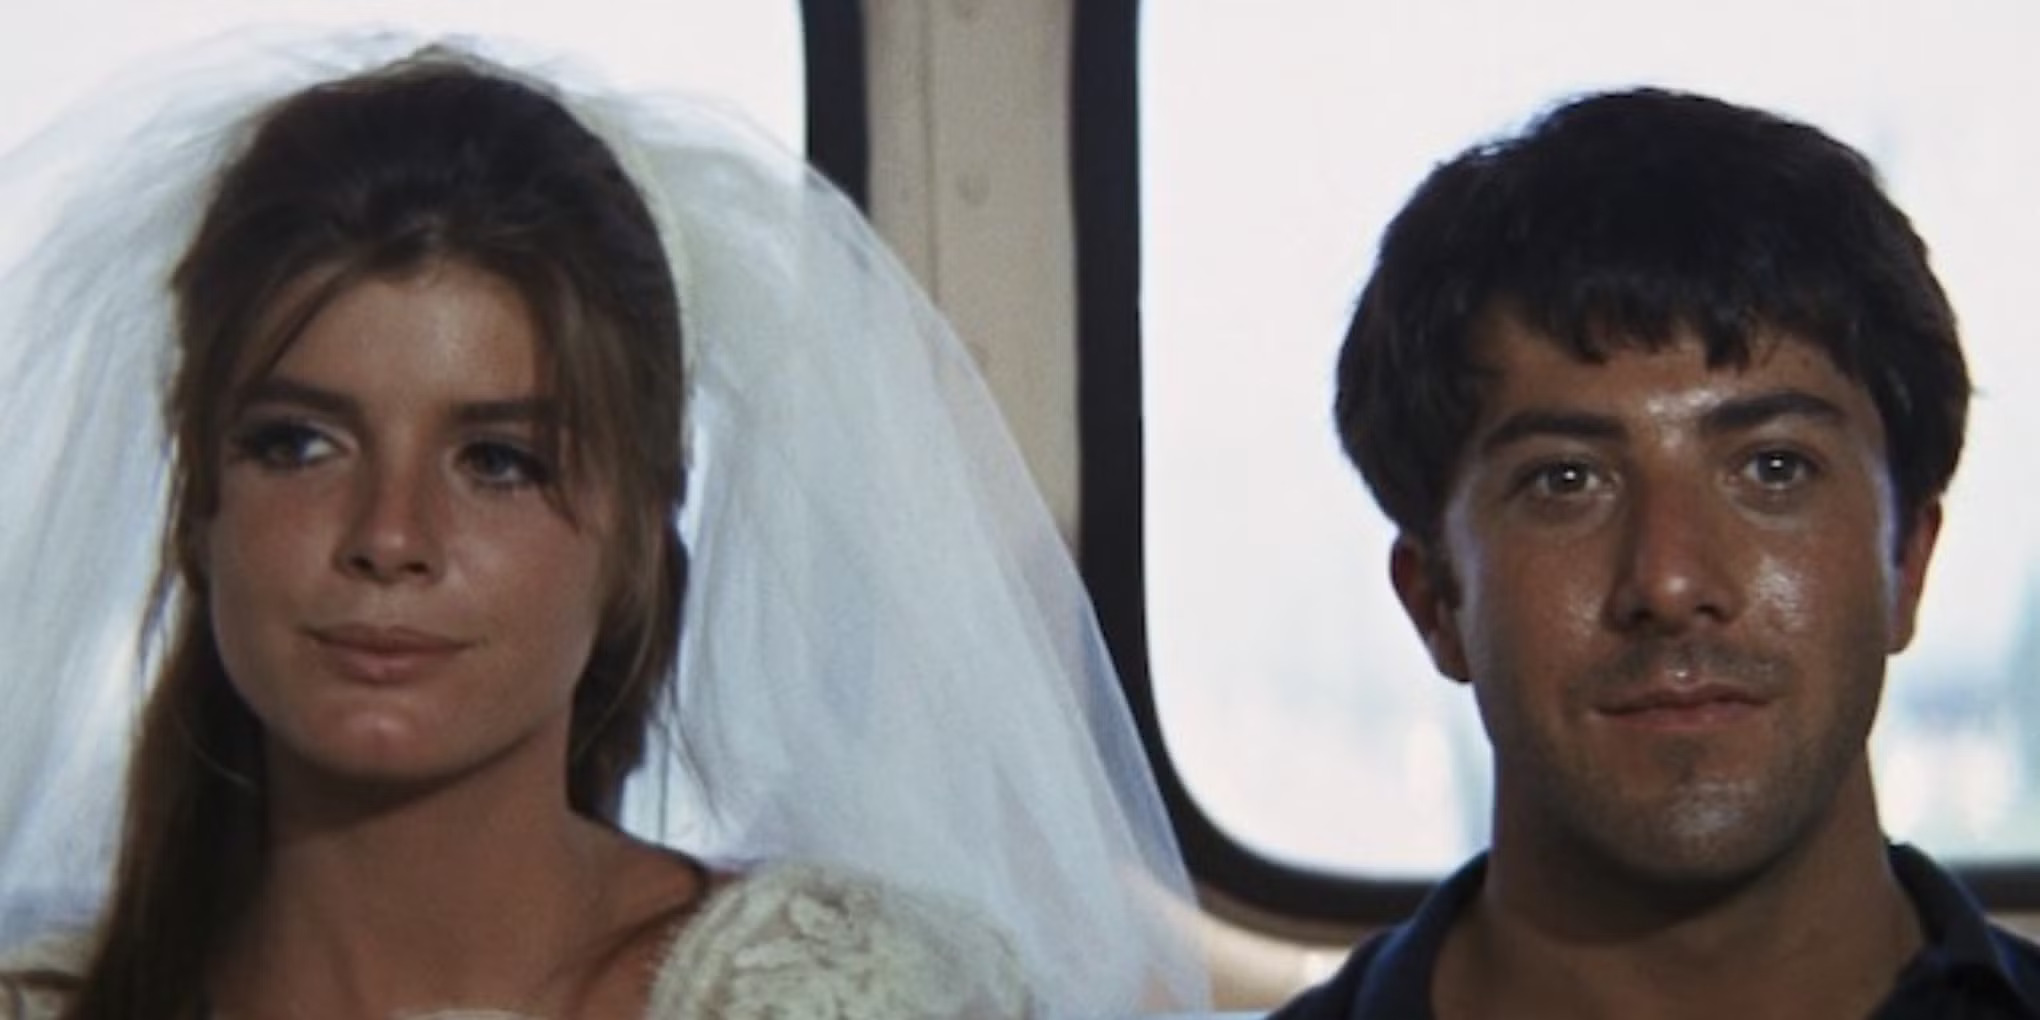
\includegraphics[width=0.55\textwidth]{../shared/images/conclusion.jpeg}
  \end{figure}
\end{frame}

\begin{frame}{Movie References by Appearance Order}
  \scriptsize
  \begin{itemize}
    \item \cite{prisonerOfAzkaban}
    \item \cite{legallyBlonde}
    \item \cite{wolfOfWallStreet}
    \item \cite{shaolinSoccer}
    \item \cite{8and12}
    \item \cite{pulpFiction}
    \item \cite{livesOfOthers}
    \item \cite{jaws}
    \item \cite{fastAndFurious6}
    \item \cite{schoolOfRock}
    \item \cite{fightClub}
    \item \cite{adjustmentBureau}
    \item \cite{memento}
    \item \cite{palmSprings}
    \item \cite{fridayNightLights}
    \item \cite{aladdin}
    \item \cite{moonriseKingdom}
    \item \cite{teamAmerica}
    \item \cite{graduate}
    \item \cite{paddington}
  \end{itemize}
  \normalsize
\end{frame}

\begin{frame}[allowframebreaks]{References}
  \scriptsize
  \bibliographystyle{../shared/asa}  % Using asa.bst for this style
  \bibliography{../shared/refs}
\end{frame}


\begin{frame}{Thank You}
  \begin{itemize}
    \item Thank you for listening!
    \item Any questions?
  \end{itemize}
  
  \begin{figure}
    
\includegraphics[width=0.75\textwidth]{../shared/images/screenshots/thanks.jpg}
  \end{figure}
\end{frame}

\begin{frame}{\cite{redOne} Adjusted Multipliers}
  \begin{figure}
    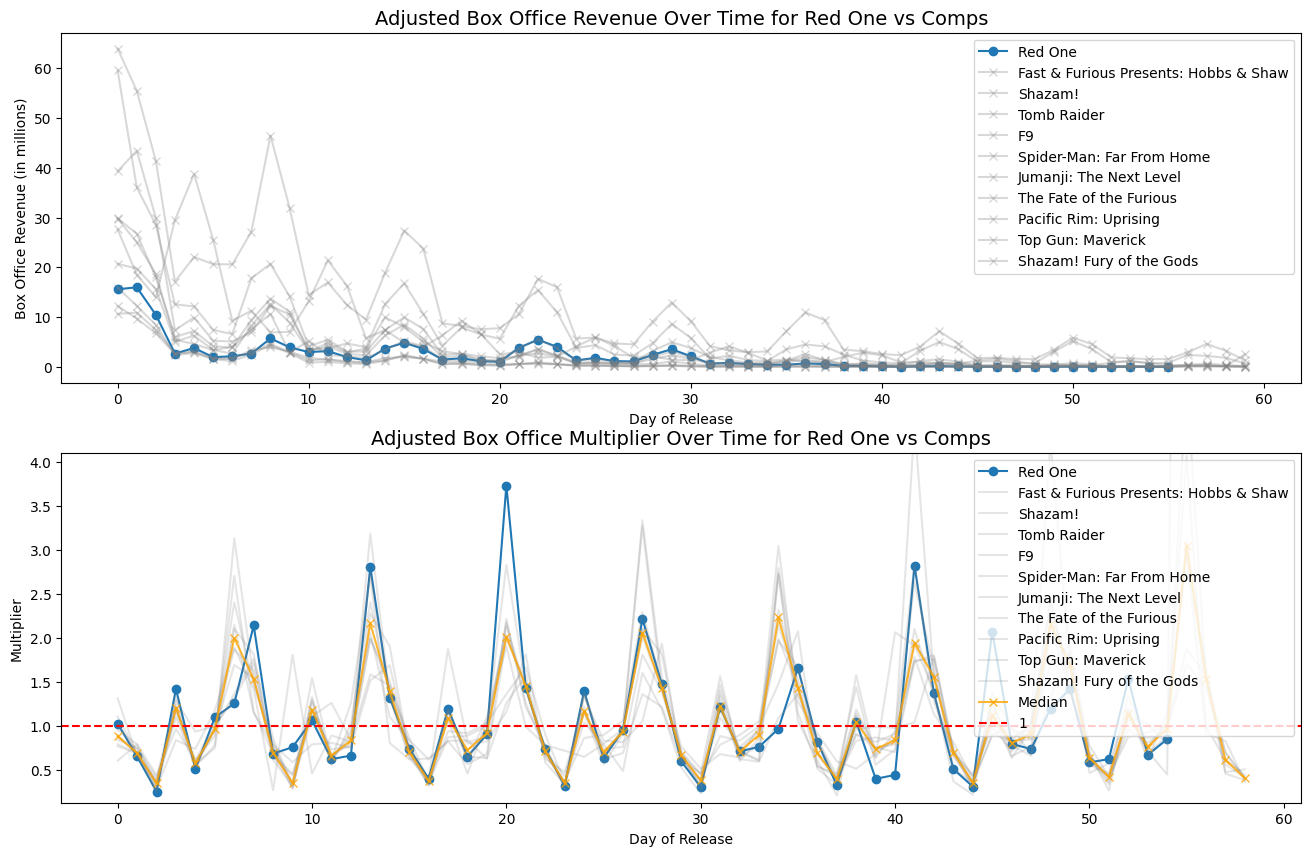
\includegraphics[width=0.92\textwidth]{../shared/images/redonecomps.png}
  \end{figure}
\end{frame}

\begin{frame}{\cite{captainAmerica}}
  \begin{figure}
    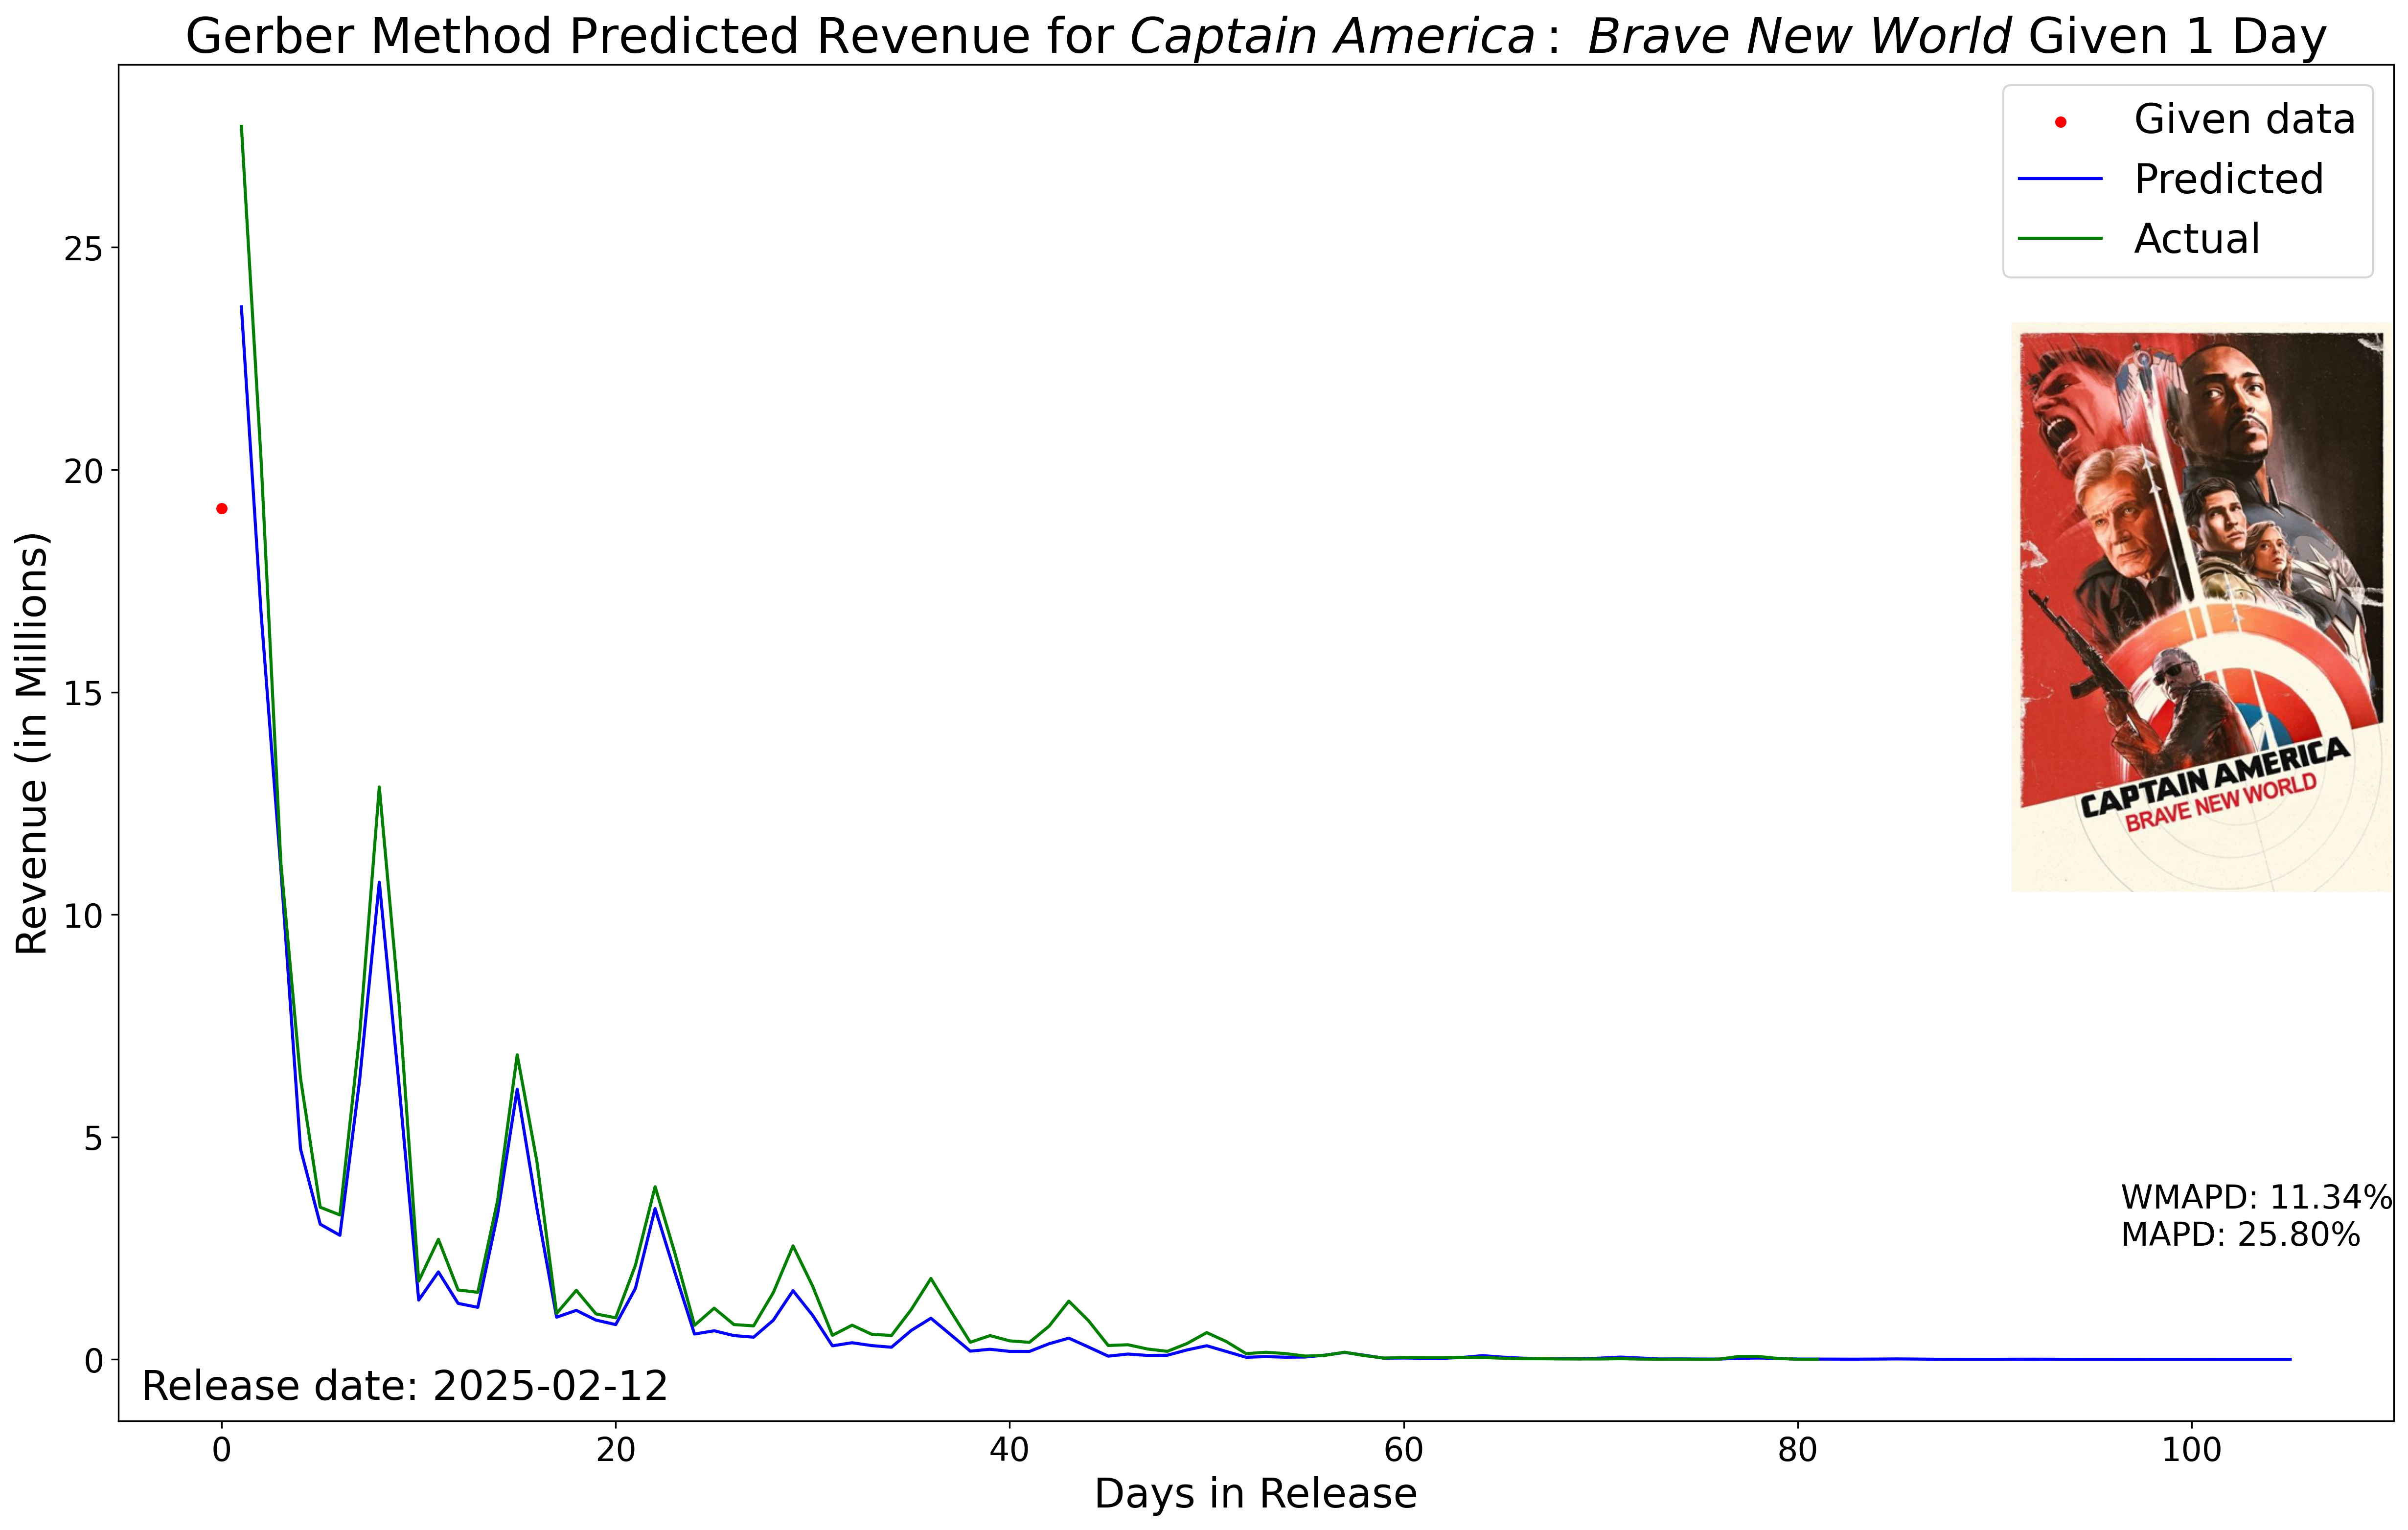
\includegraphics[width=0.95\textwidth]{../shared/images/pred/Captain America: Brave New World_1.png}
  \end{figure}
\end{frame}

\begin{frame}{Results Multiple: \cite{barbie}}
  \begin{figure}
    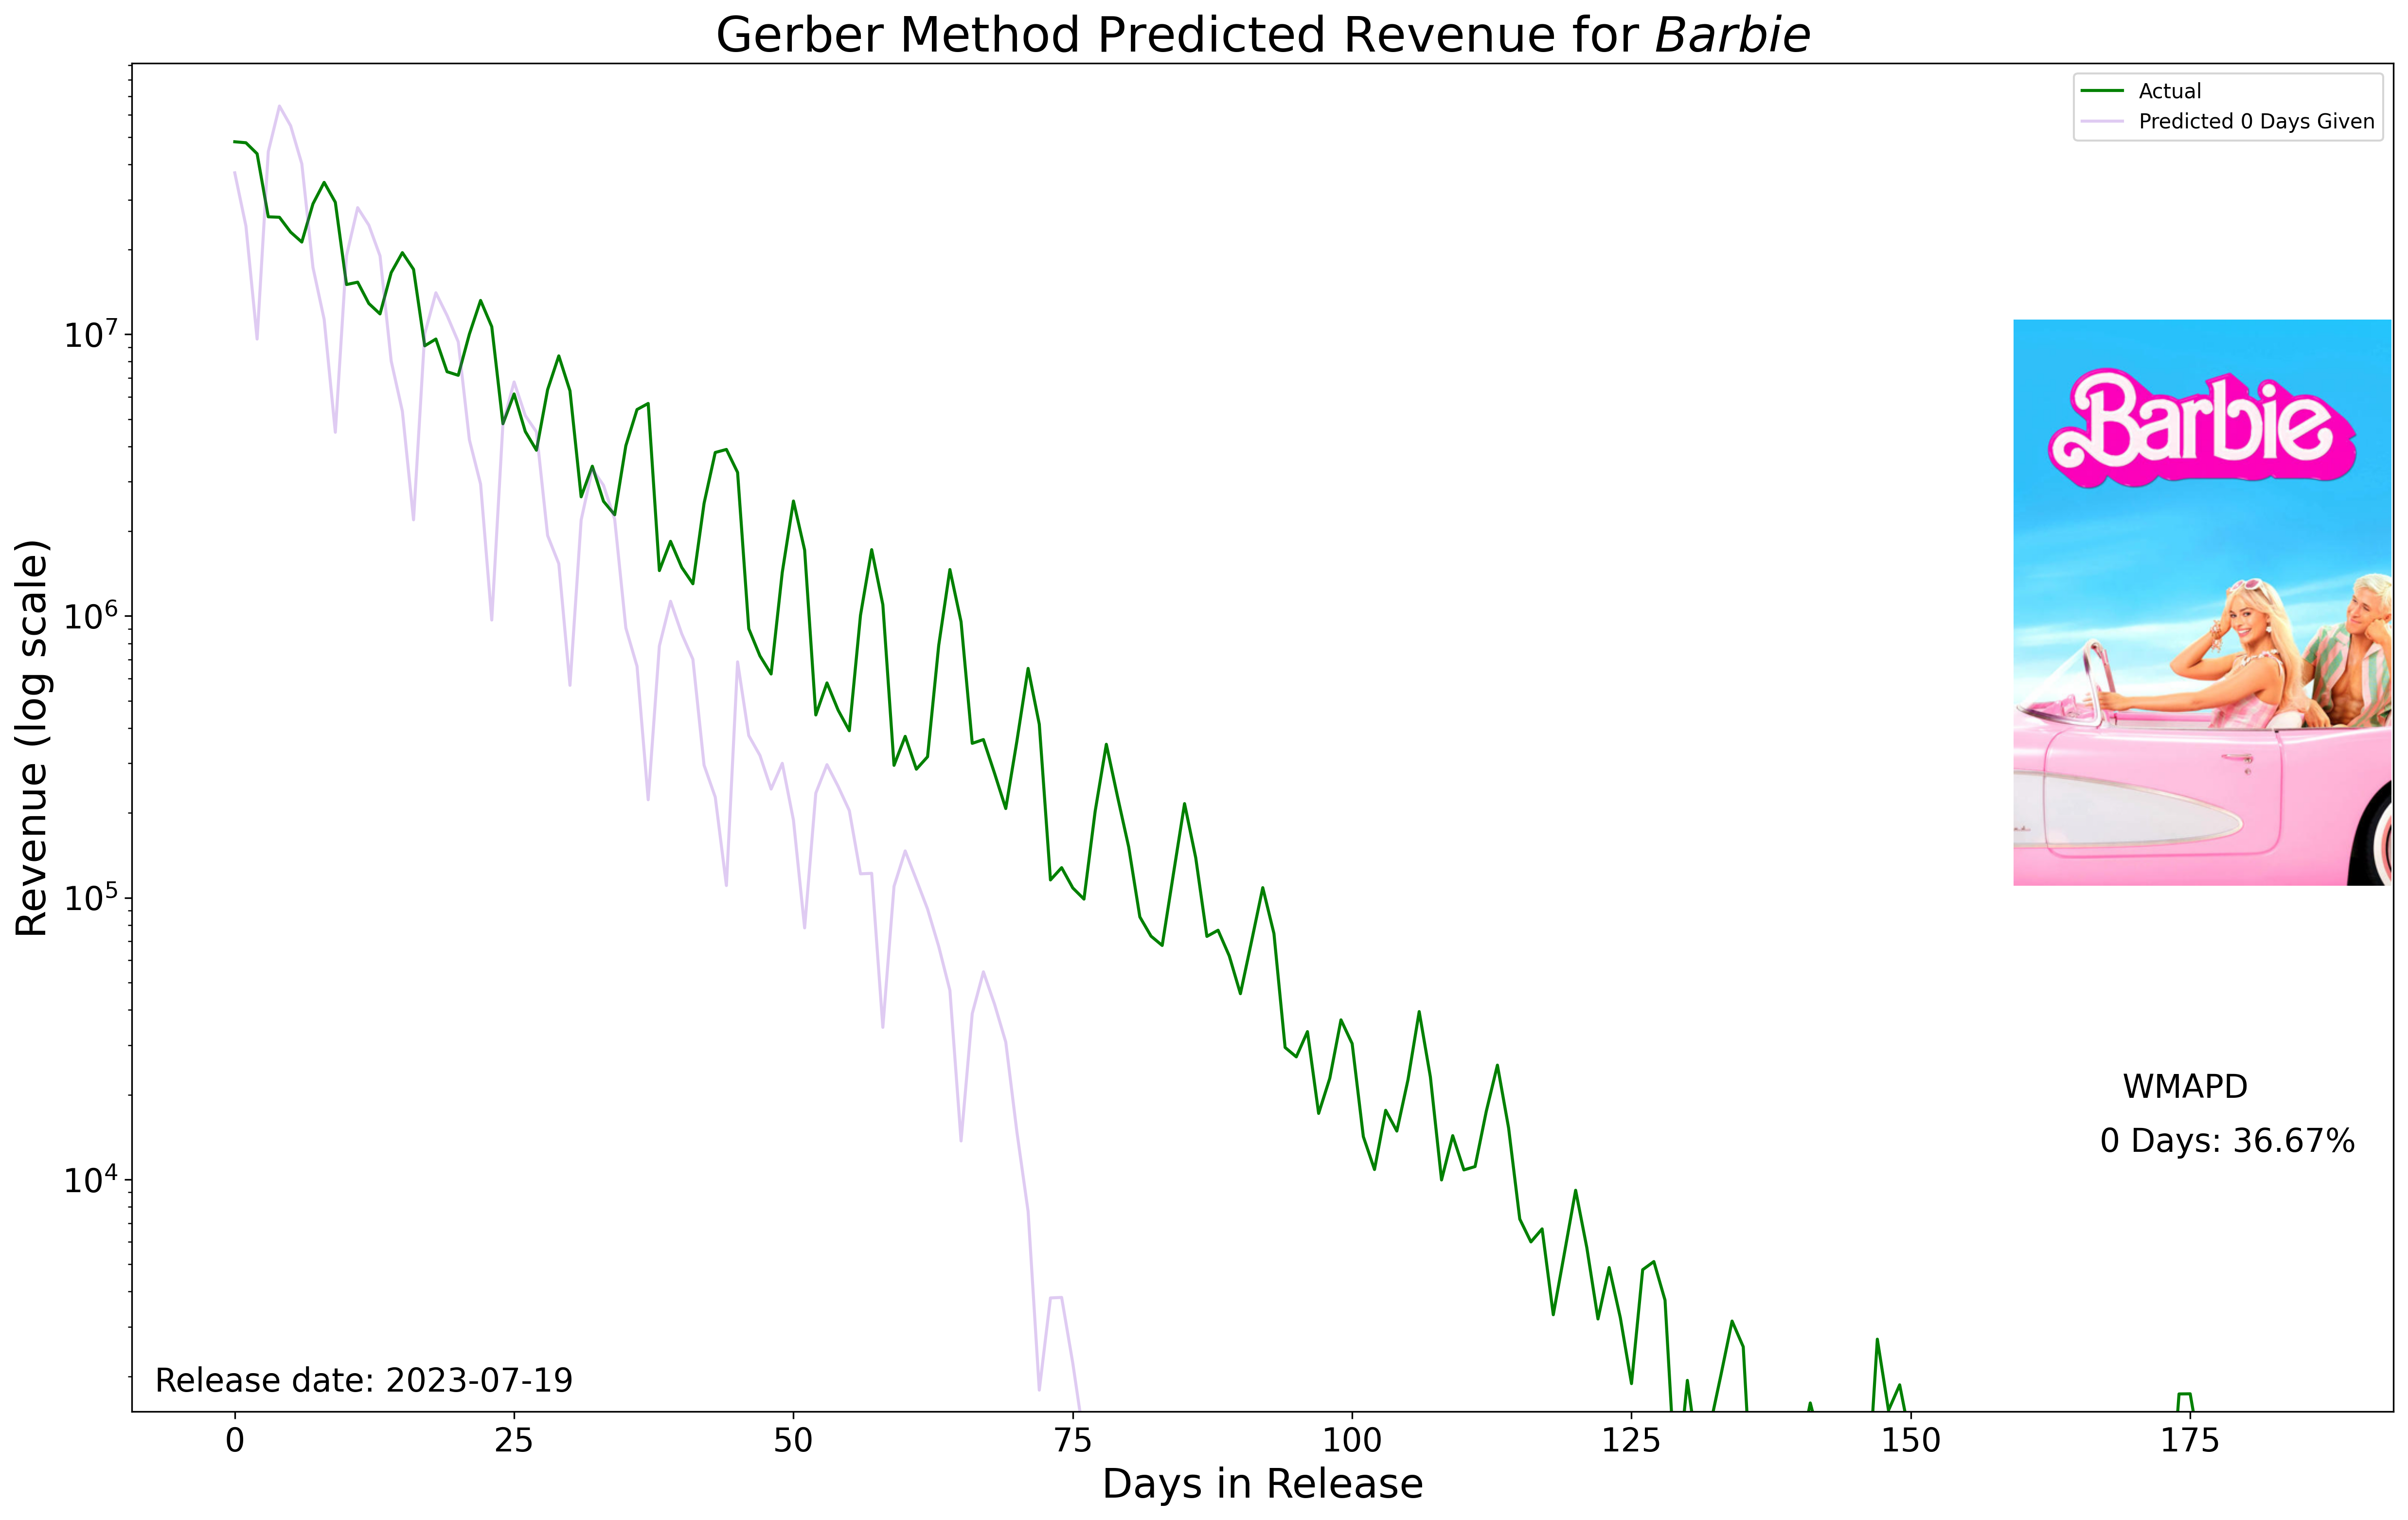
\includegraphics[width=0.95\textwidth]{../shared/images/pred/Barbie_multiple_1.png}
  \end{figure}
\end{frame}

\begin{frame}{Results Multiple: \cite{barbie}}
  \begin{figure}
    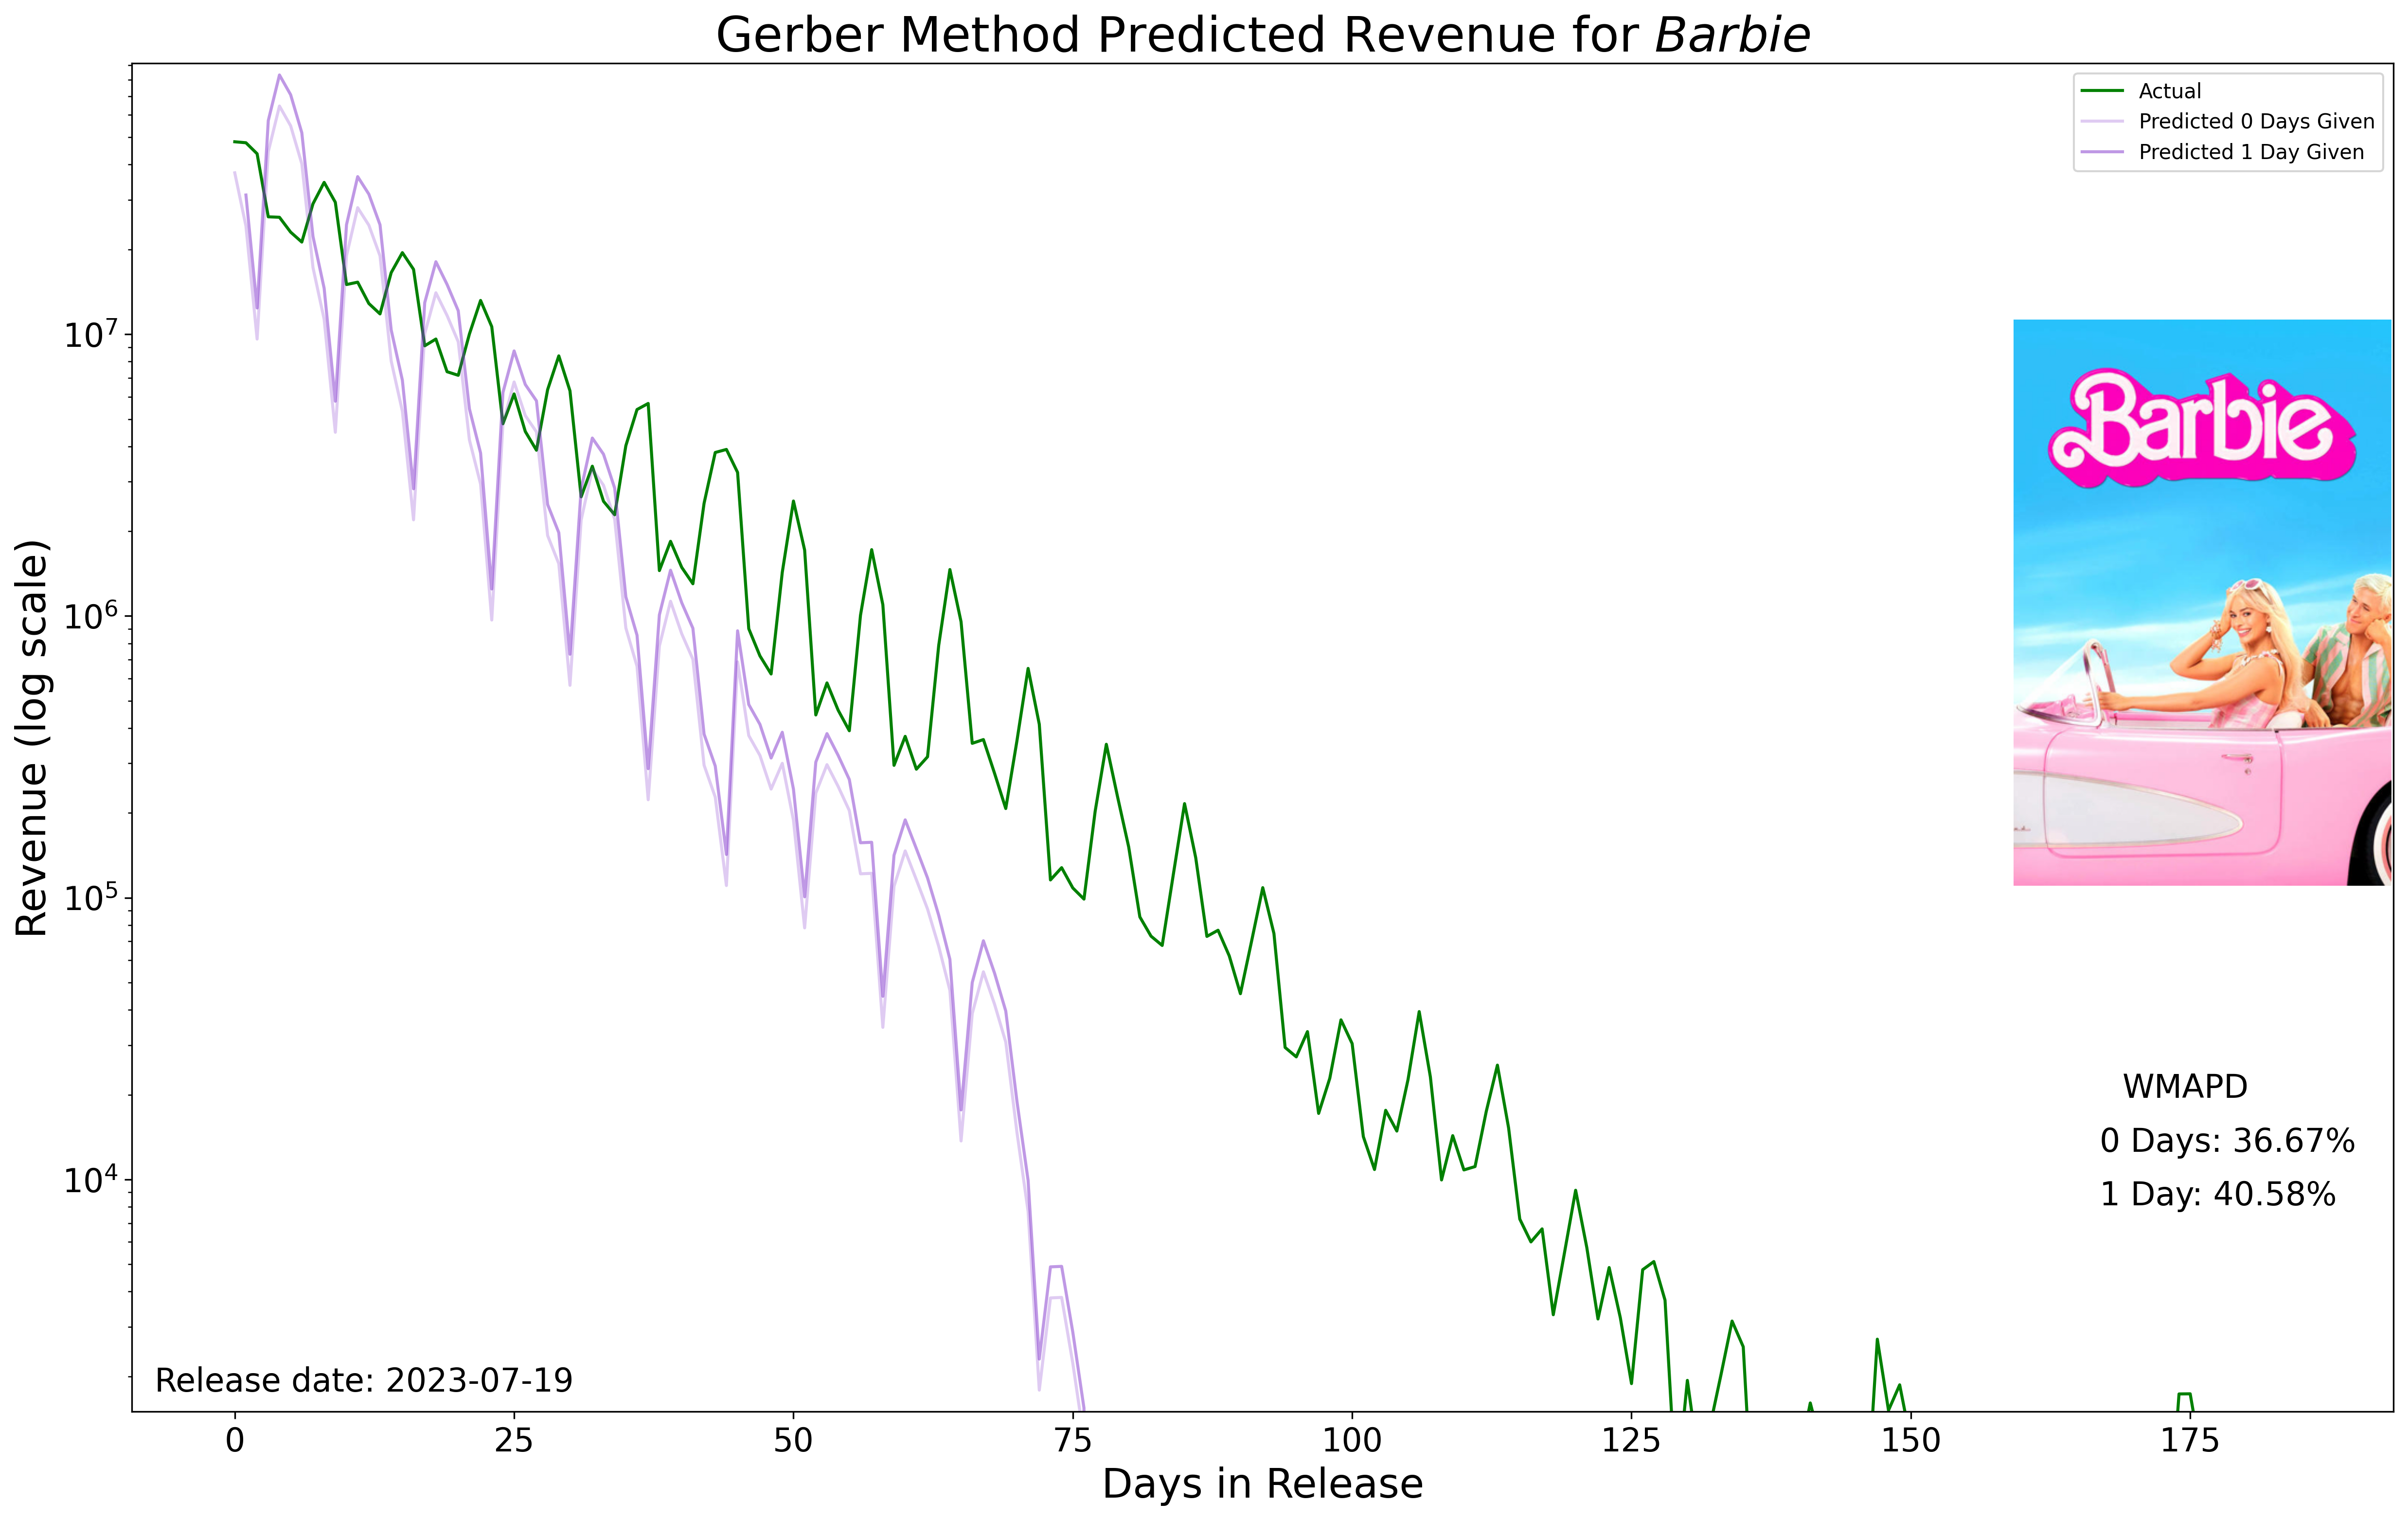
\includegraphics[width=0.95\textwidth]{../shared/images/pred/Barbie_multiple_2.png}
  \end{figure}
  \addtocounter{framenumber}{-1}
\end{frame}

\begin{frame}{Results Multiple: \cite{barbie}}
  \begin{figure}
    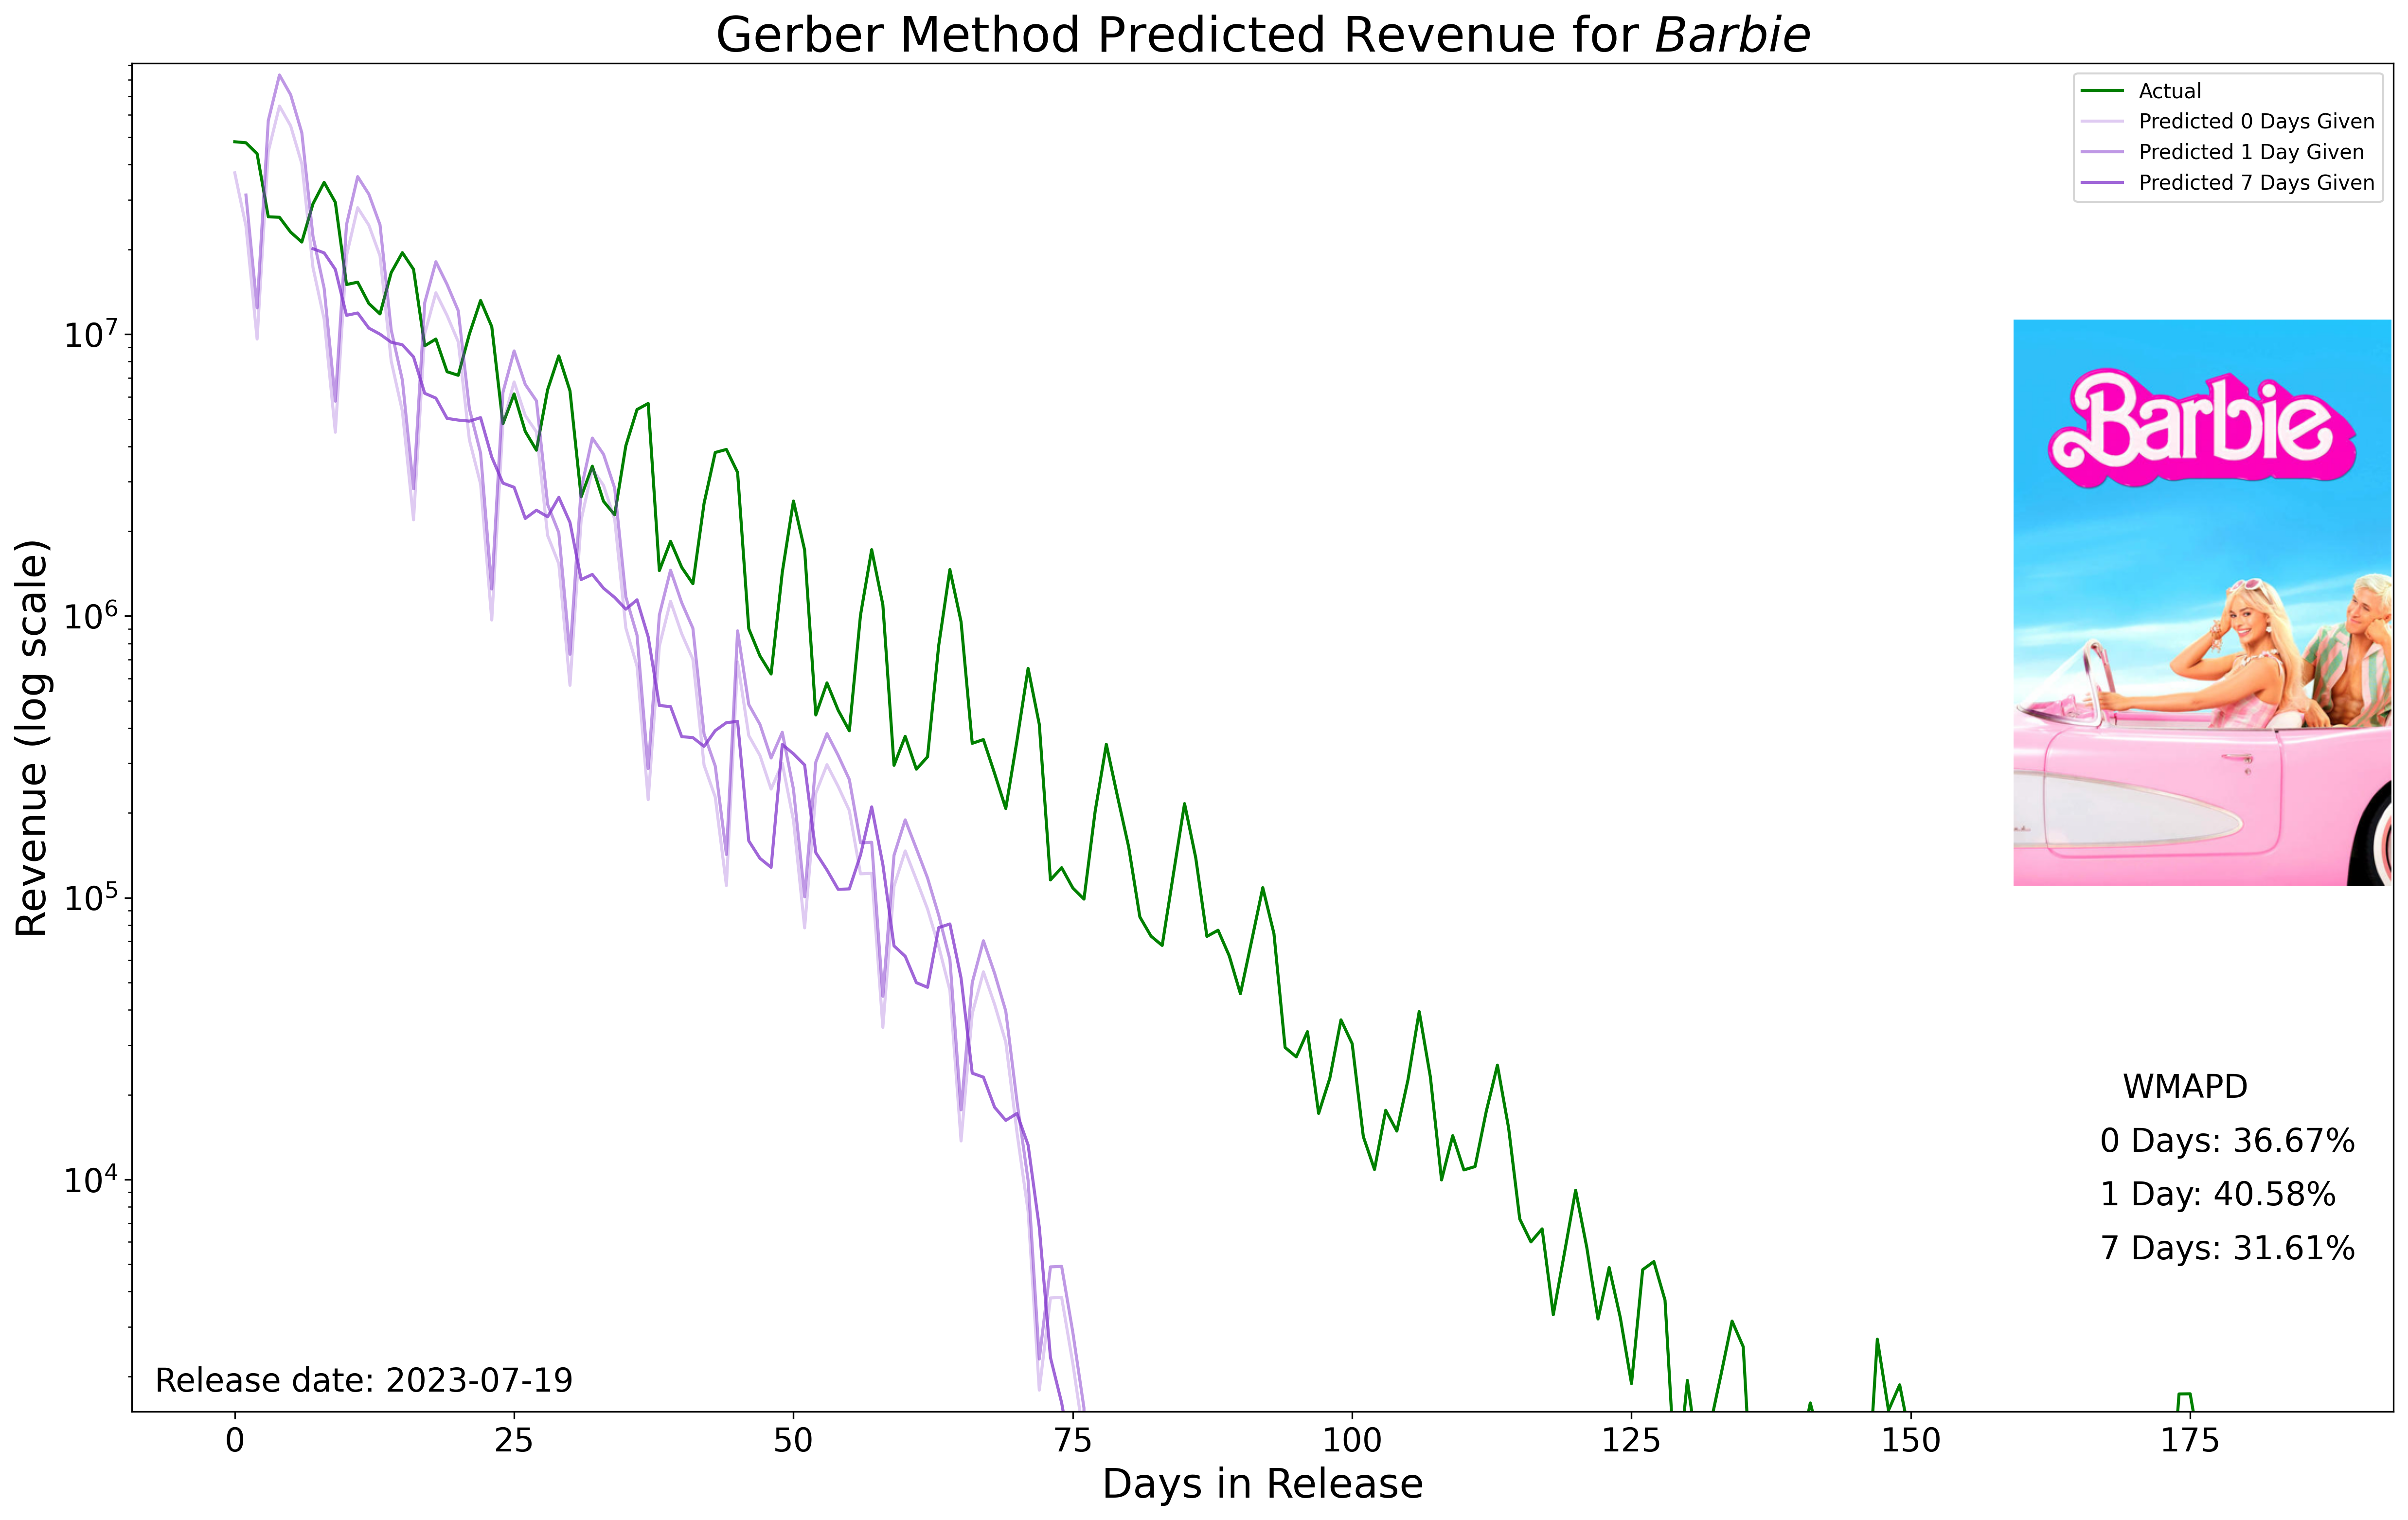
\includegraphics[width=0.95\textwidth]{../shared/images/pred/Barbie_multiple_3.png}
  \end{figure}
  \addtocounter{framenumber}{-1}
\end{frame}

\begin{frame}{Results Multiple: \cite{barbie}}
  \begin{figure}
    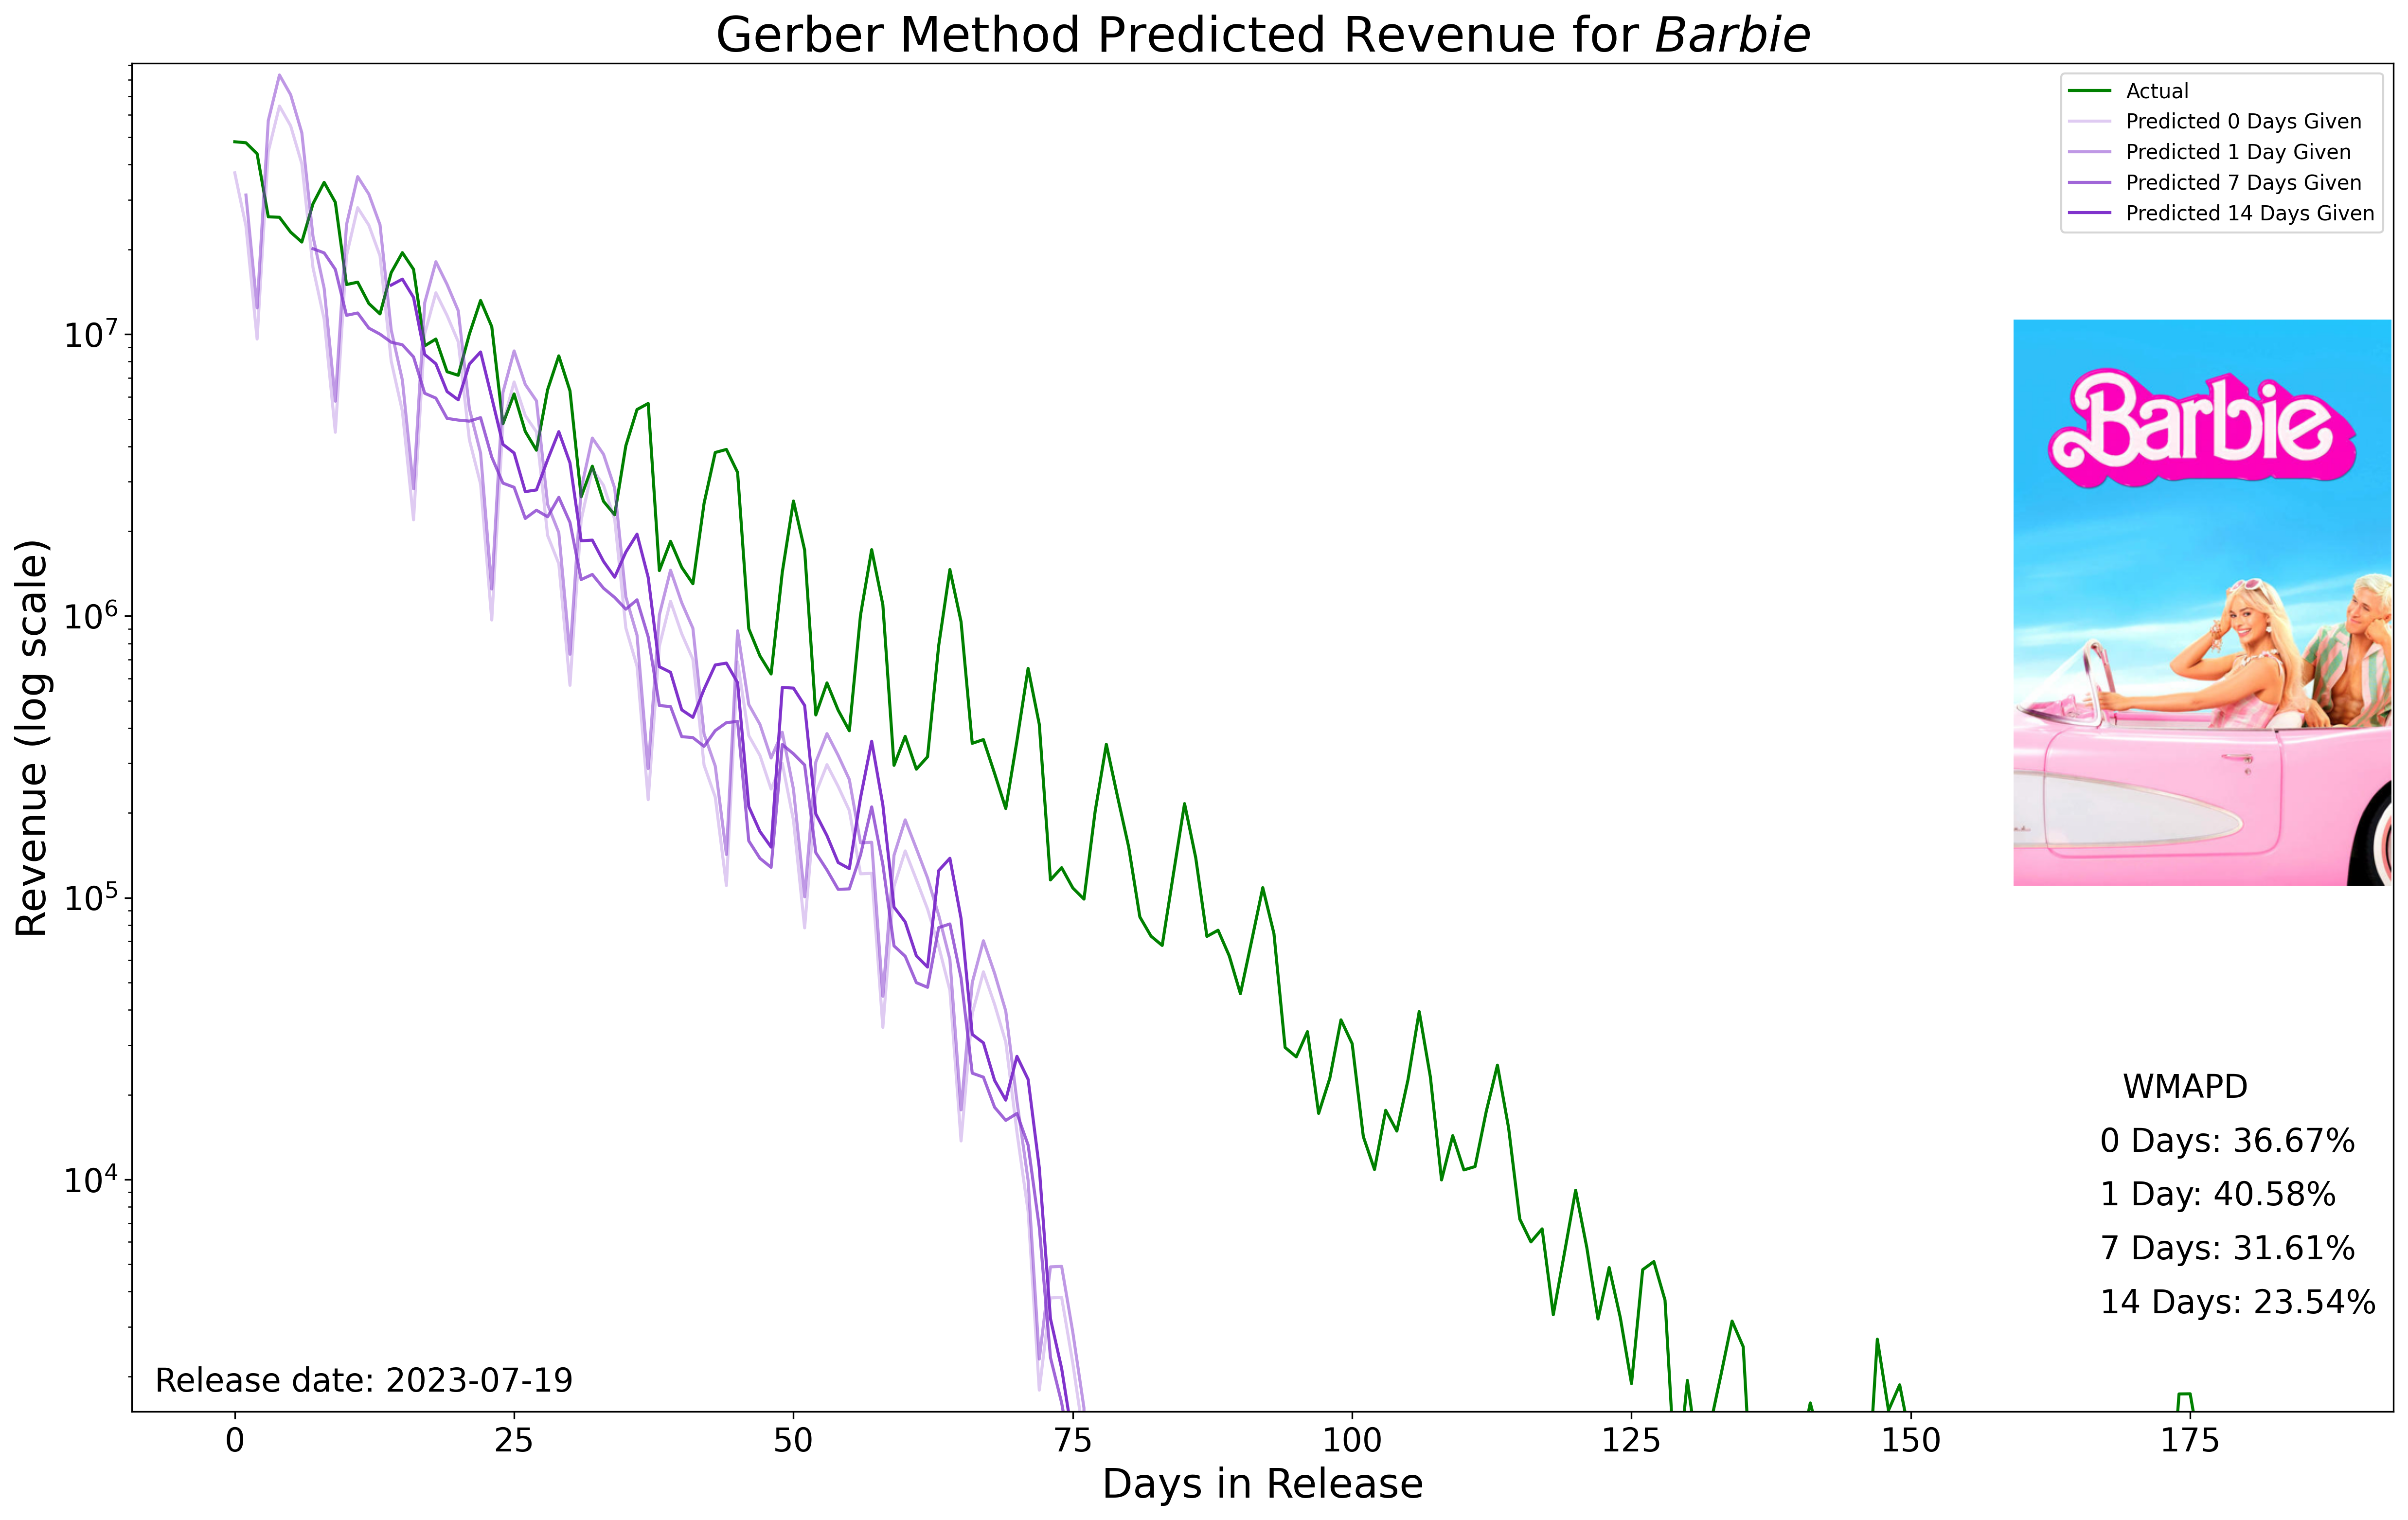
\includegraphics[width=0.95\textwidth]{../shared/images/pred/Barbie_multiple_4.png}
  \end{figure}
  \addtocounter{framenumber}{-1}
\end{frame}

\begin{frame}{Results Multiple: \cite{transformersOne}}
  \begin{figure}
    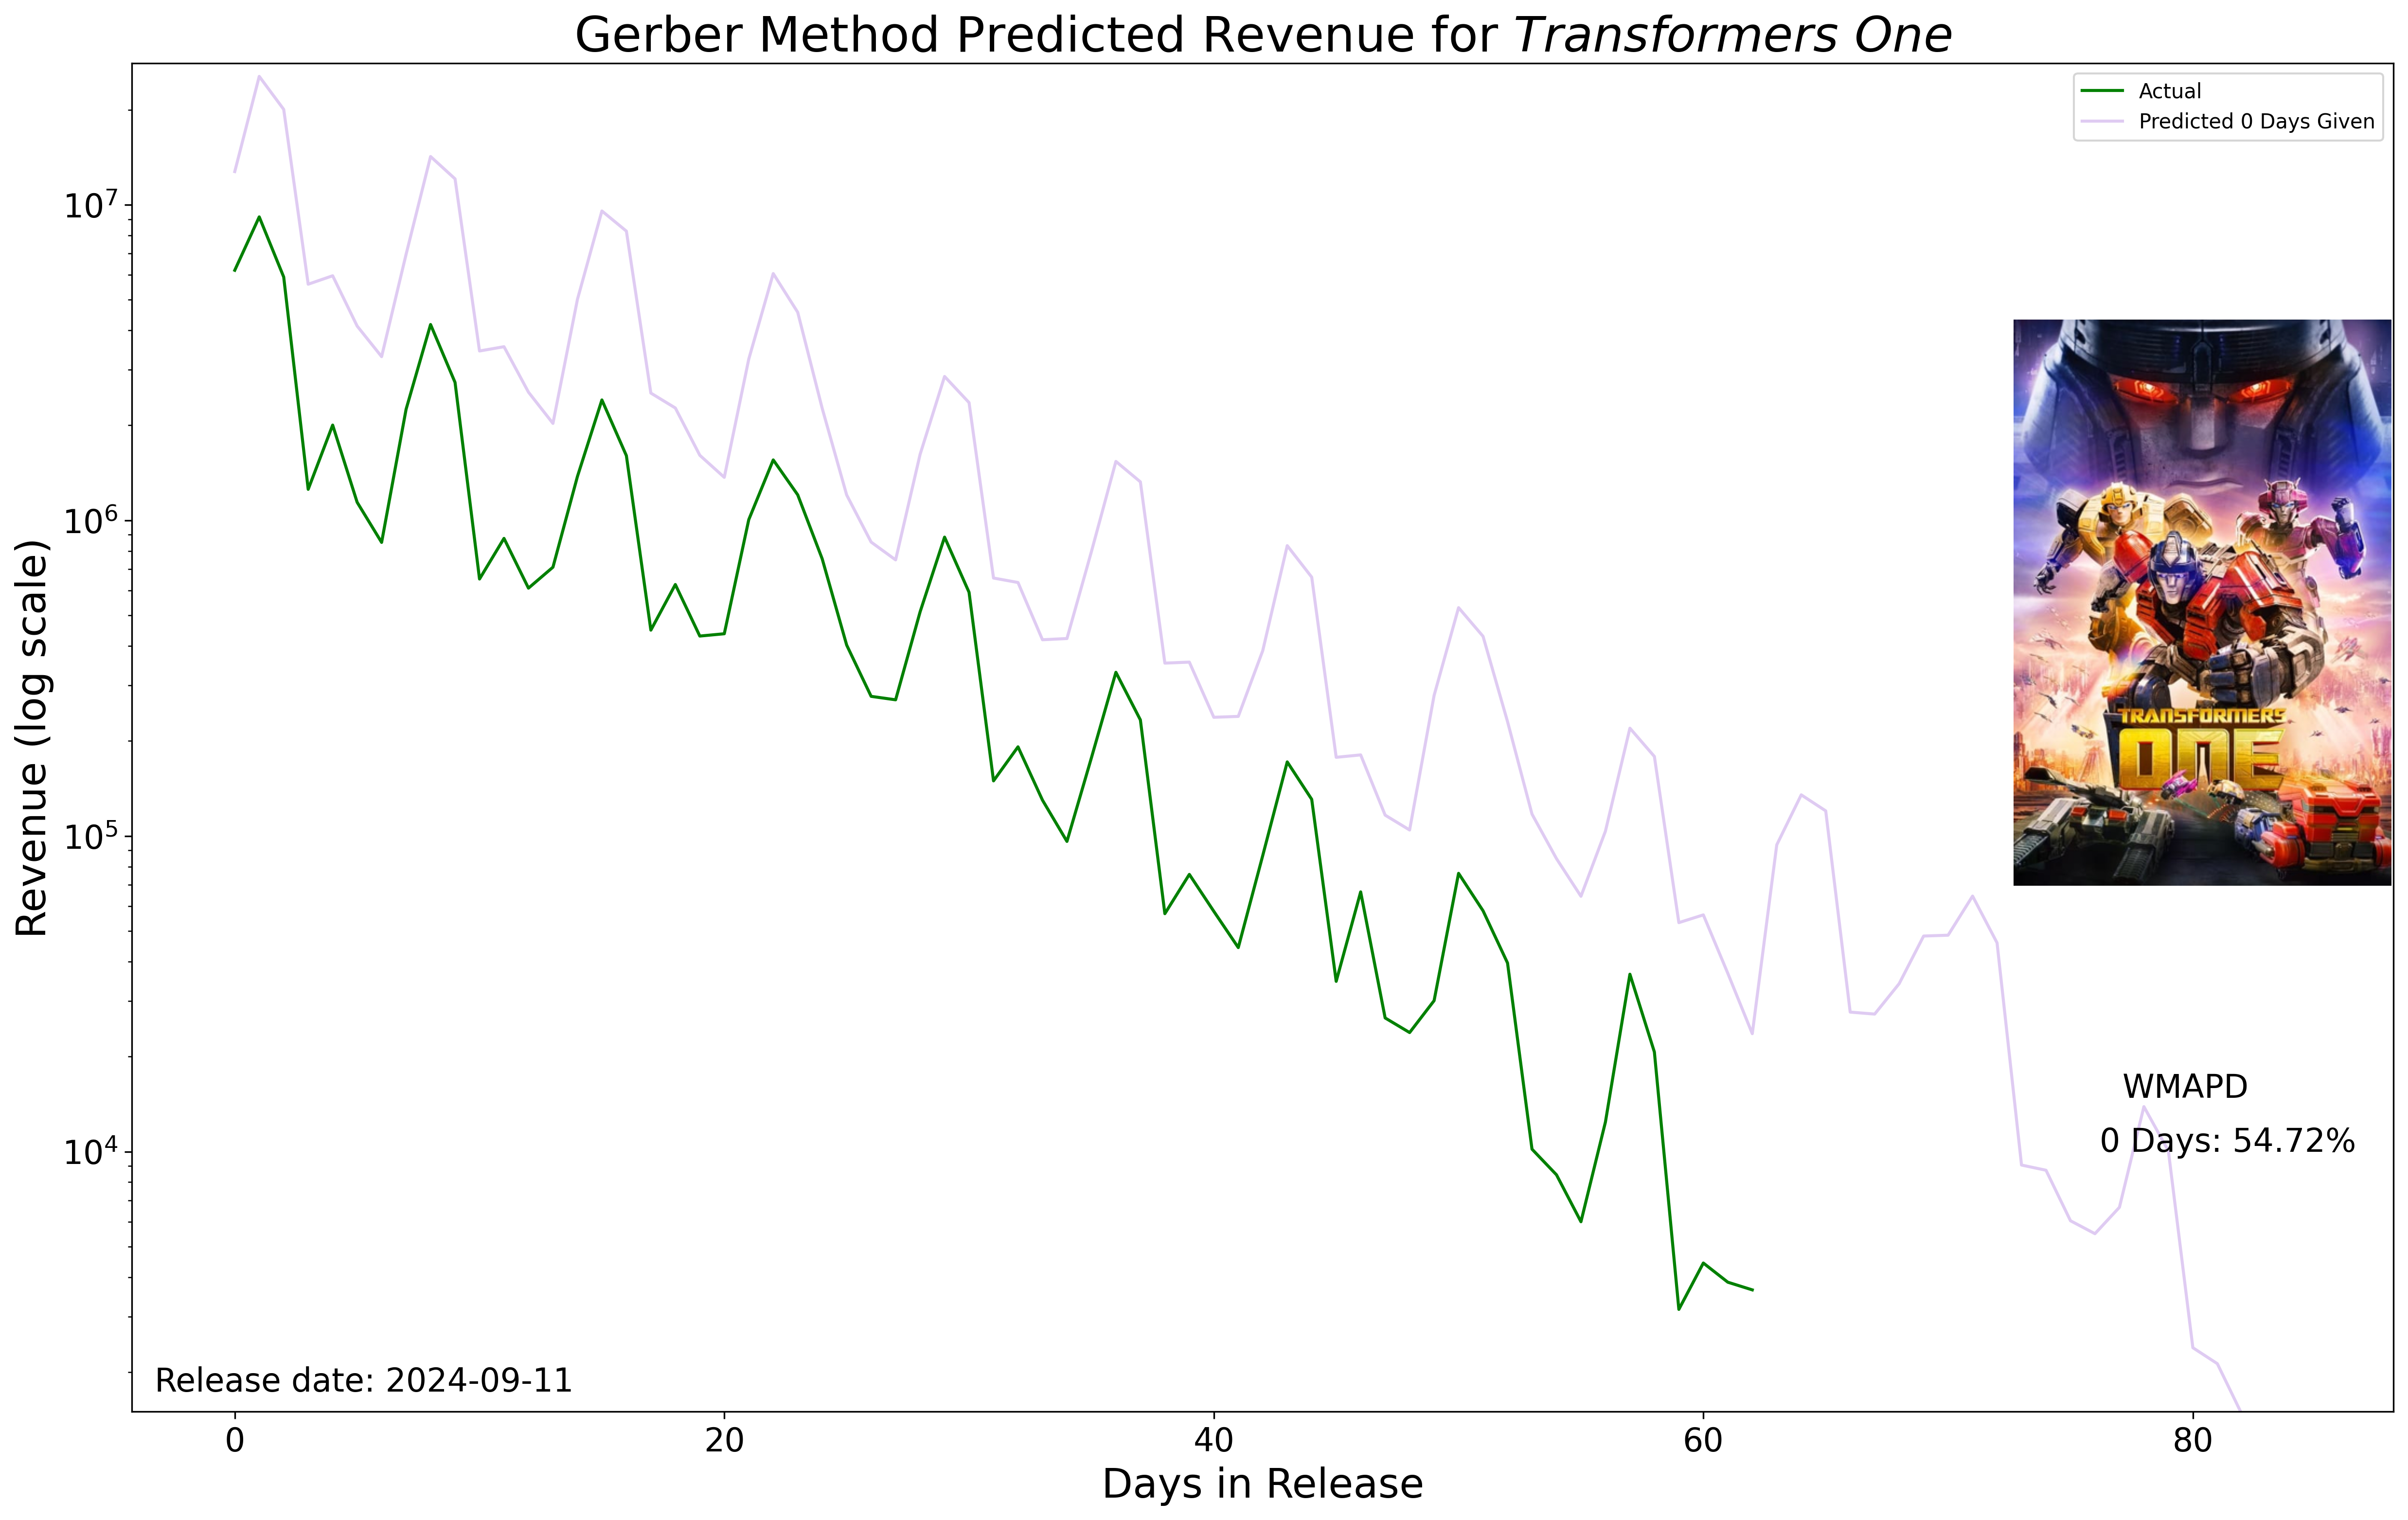
\includegraphics[width=0.95\textwidth]{../shared/images/pred/Transformers One_multiple_1.png}
  \end{figure}
\end{frame}

\begin{frame}{Results Multiple: \cite{transformersOne}}
  \begin{figure}
    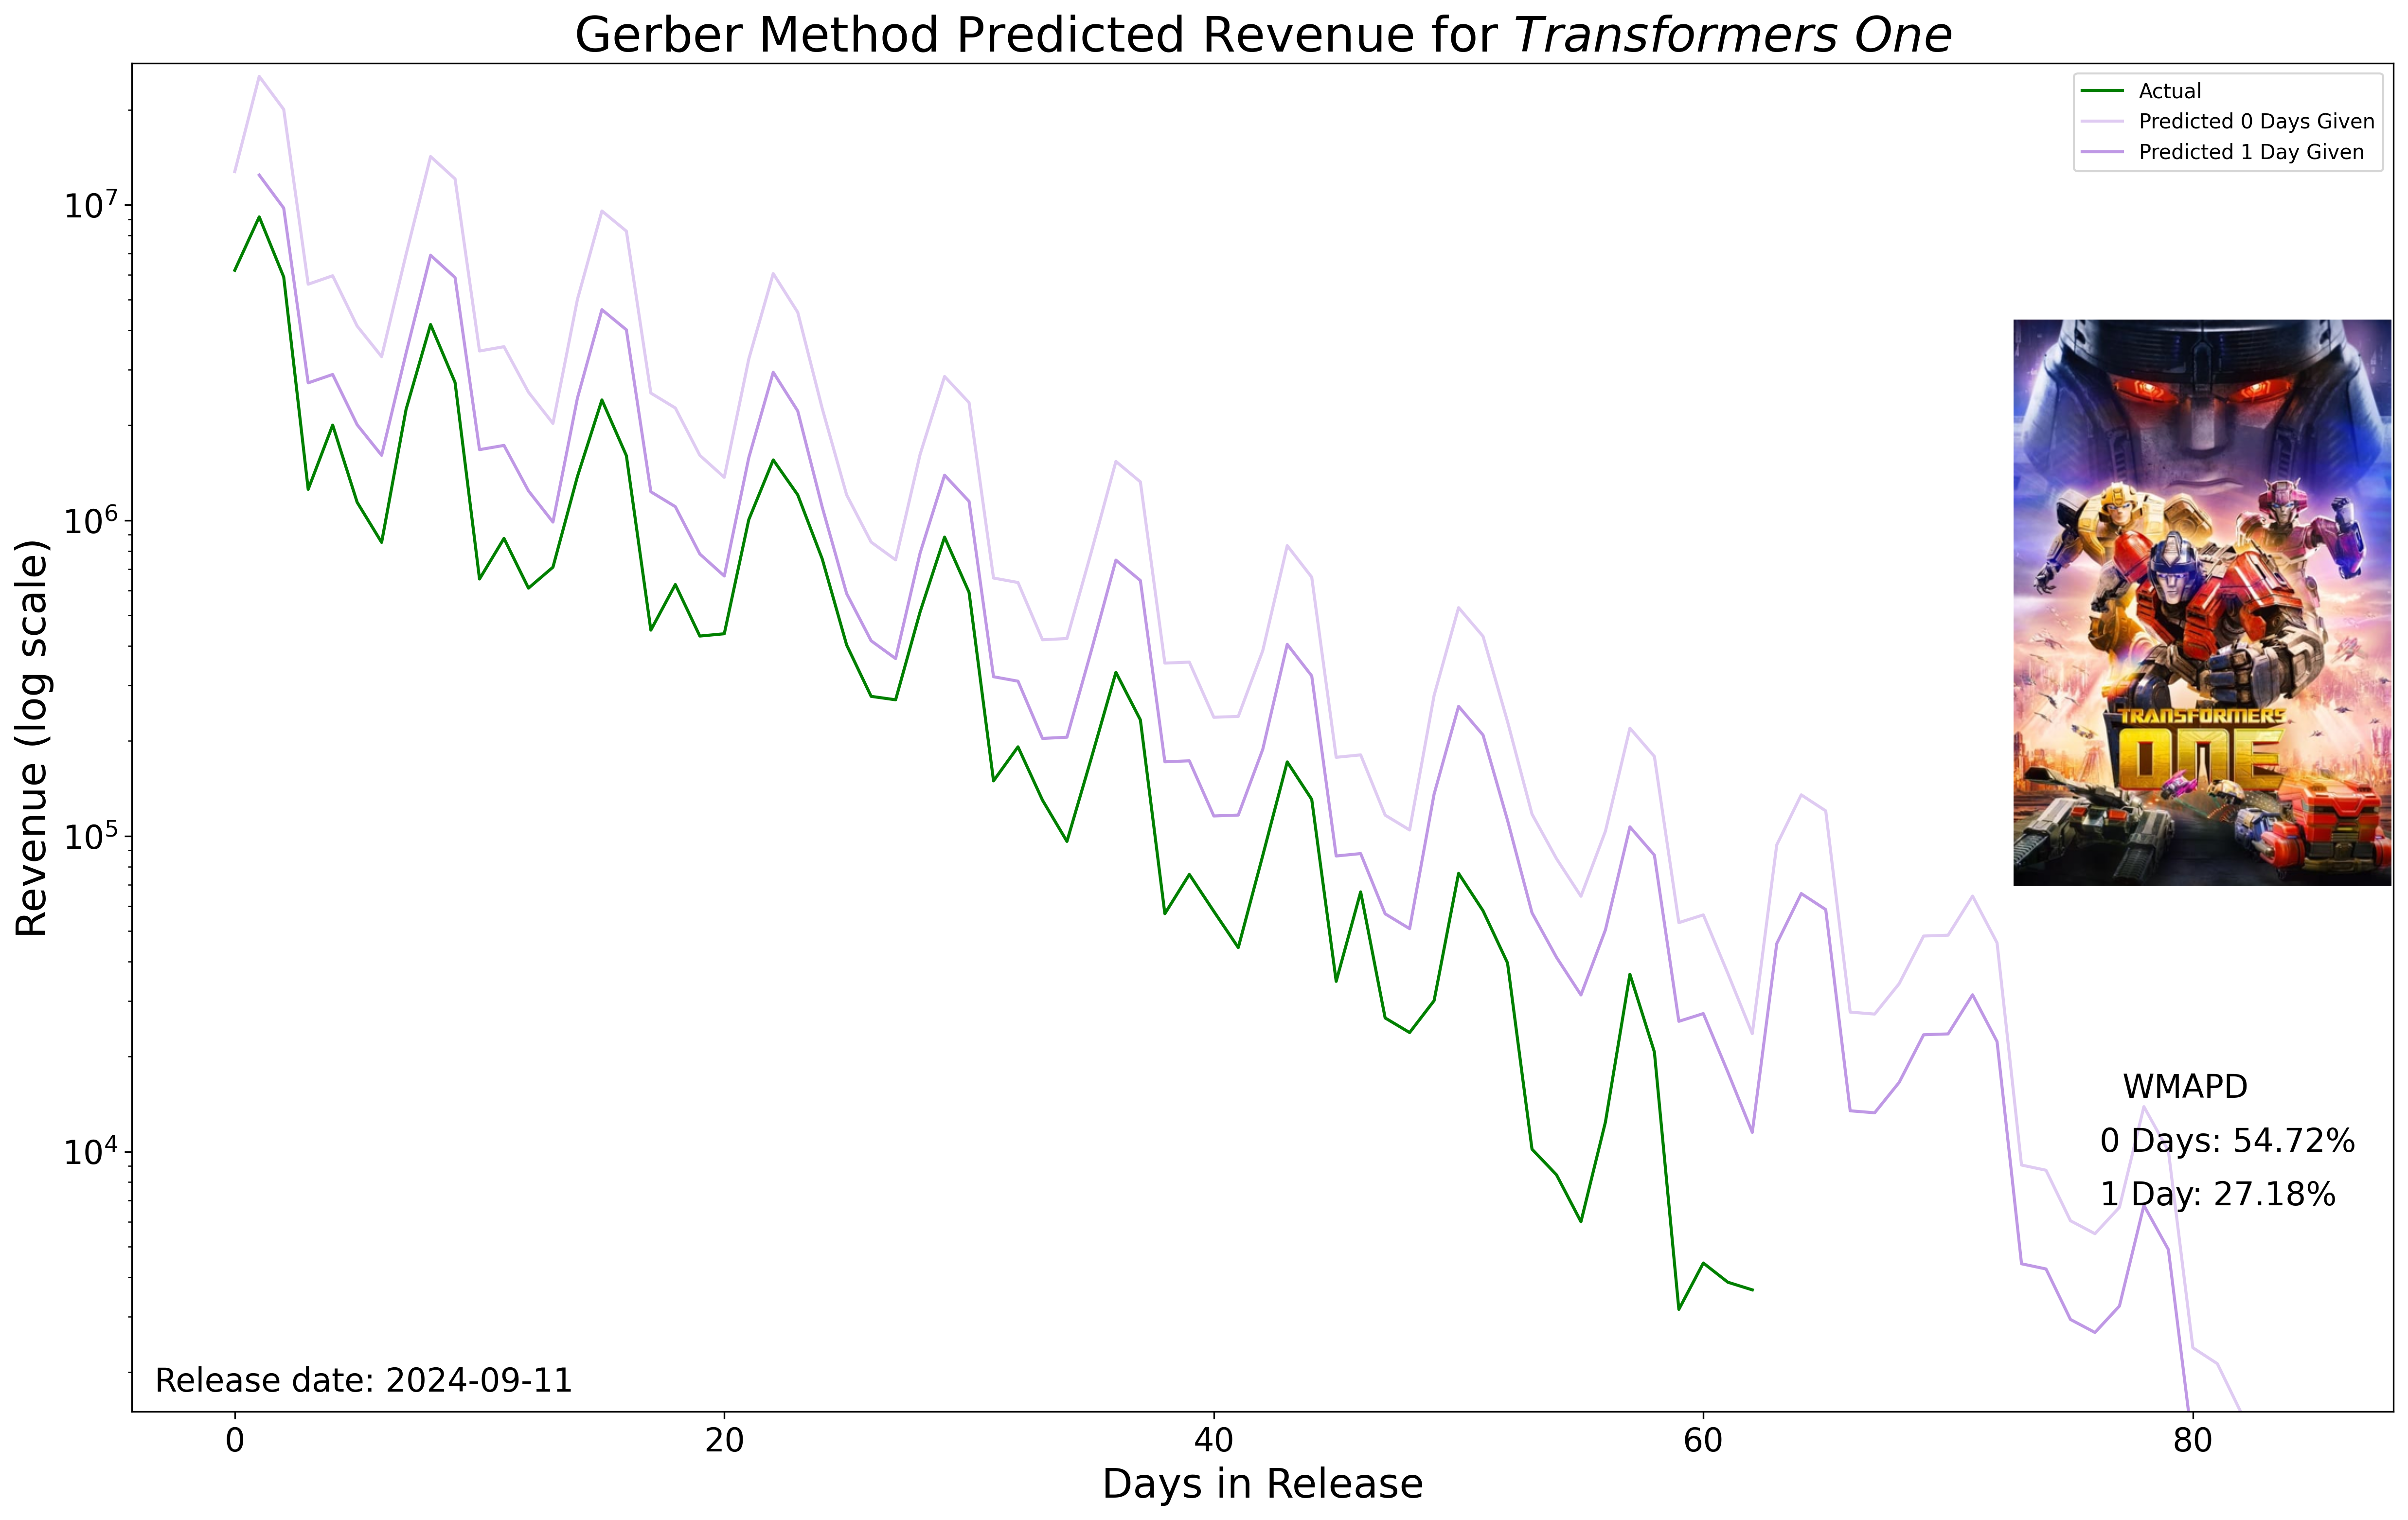
\includegraphics[width=0.95\textwidth]{../shared/images/pred/Transformers One_multiple_2.png}
  \end{figure}
  \addtocounter{framenumber}{-1}
\end{frame}

\begin{frame}{Results Multiple: \cite{transformersOne}}
  \begin{figure}
    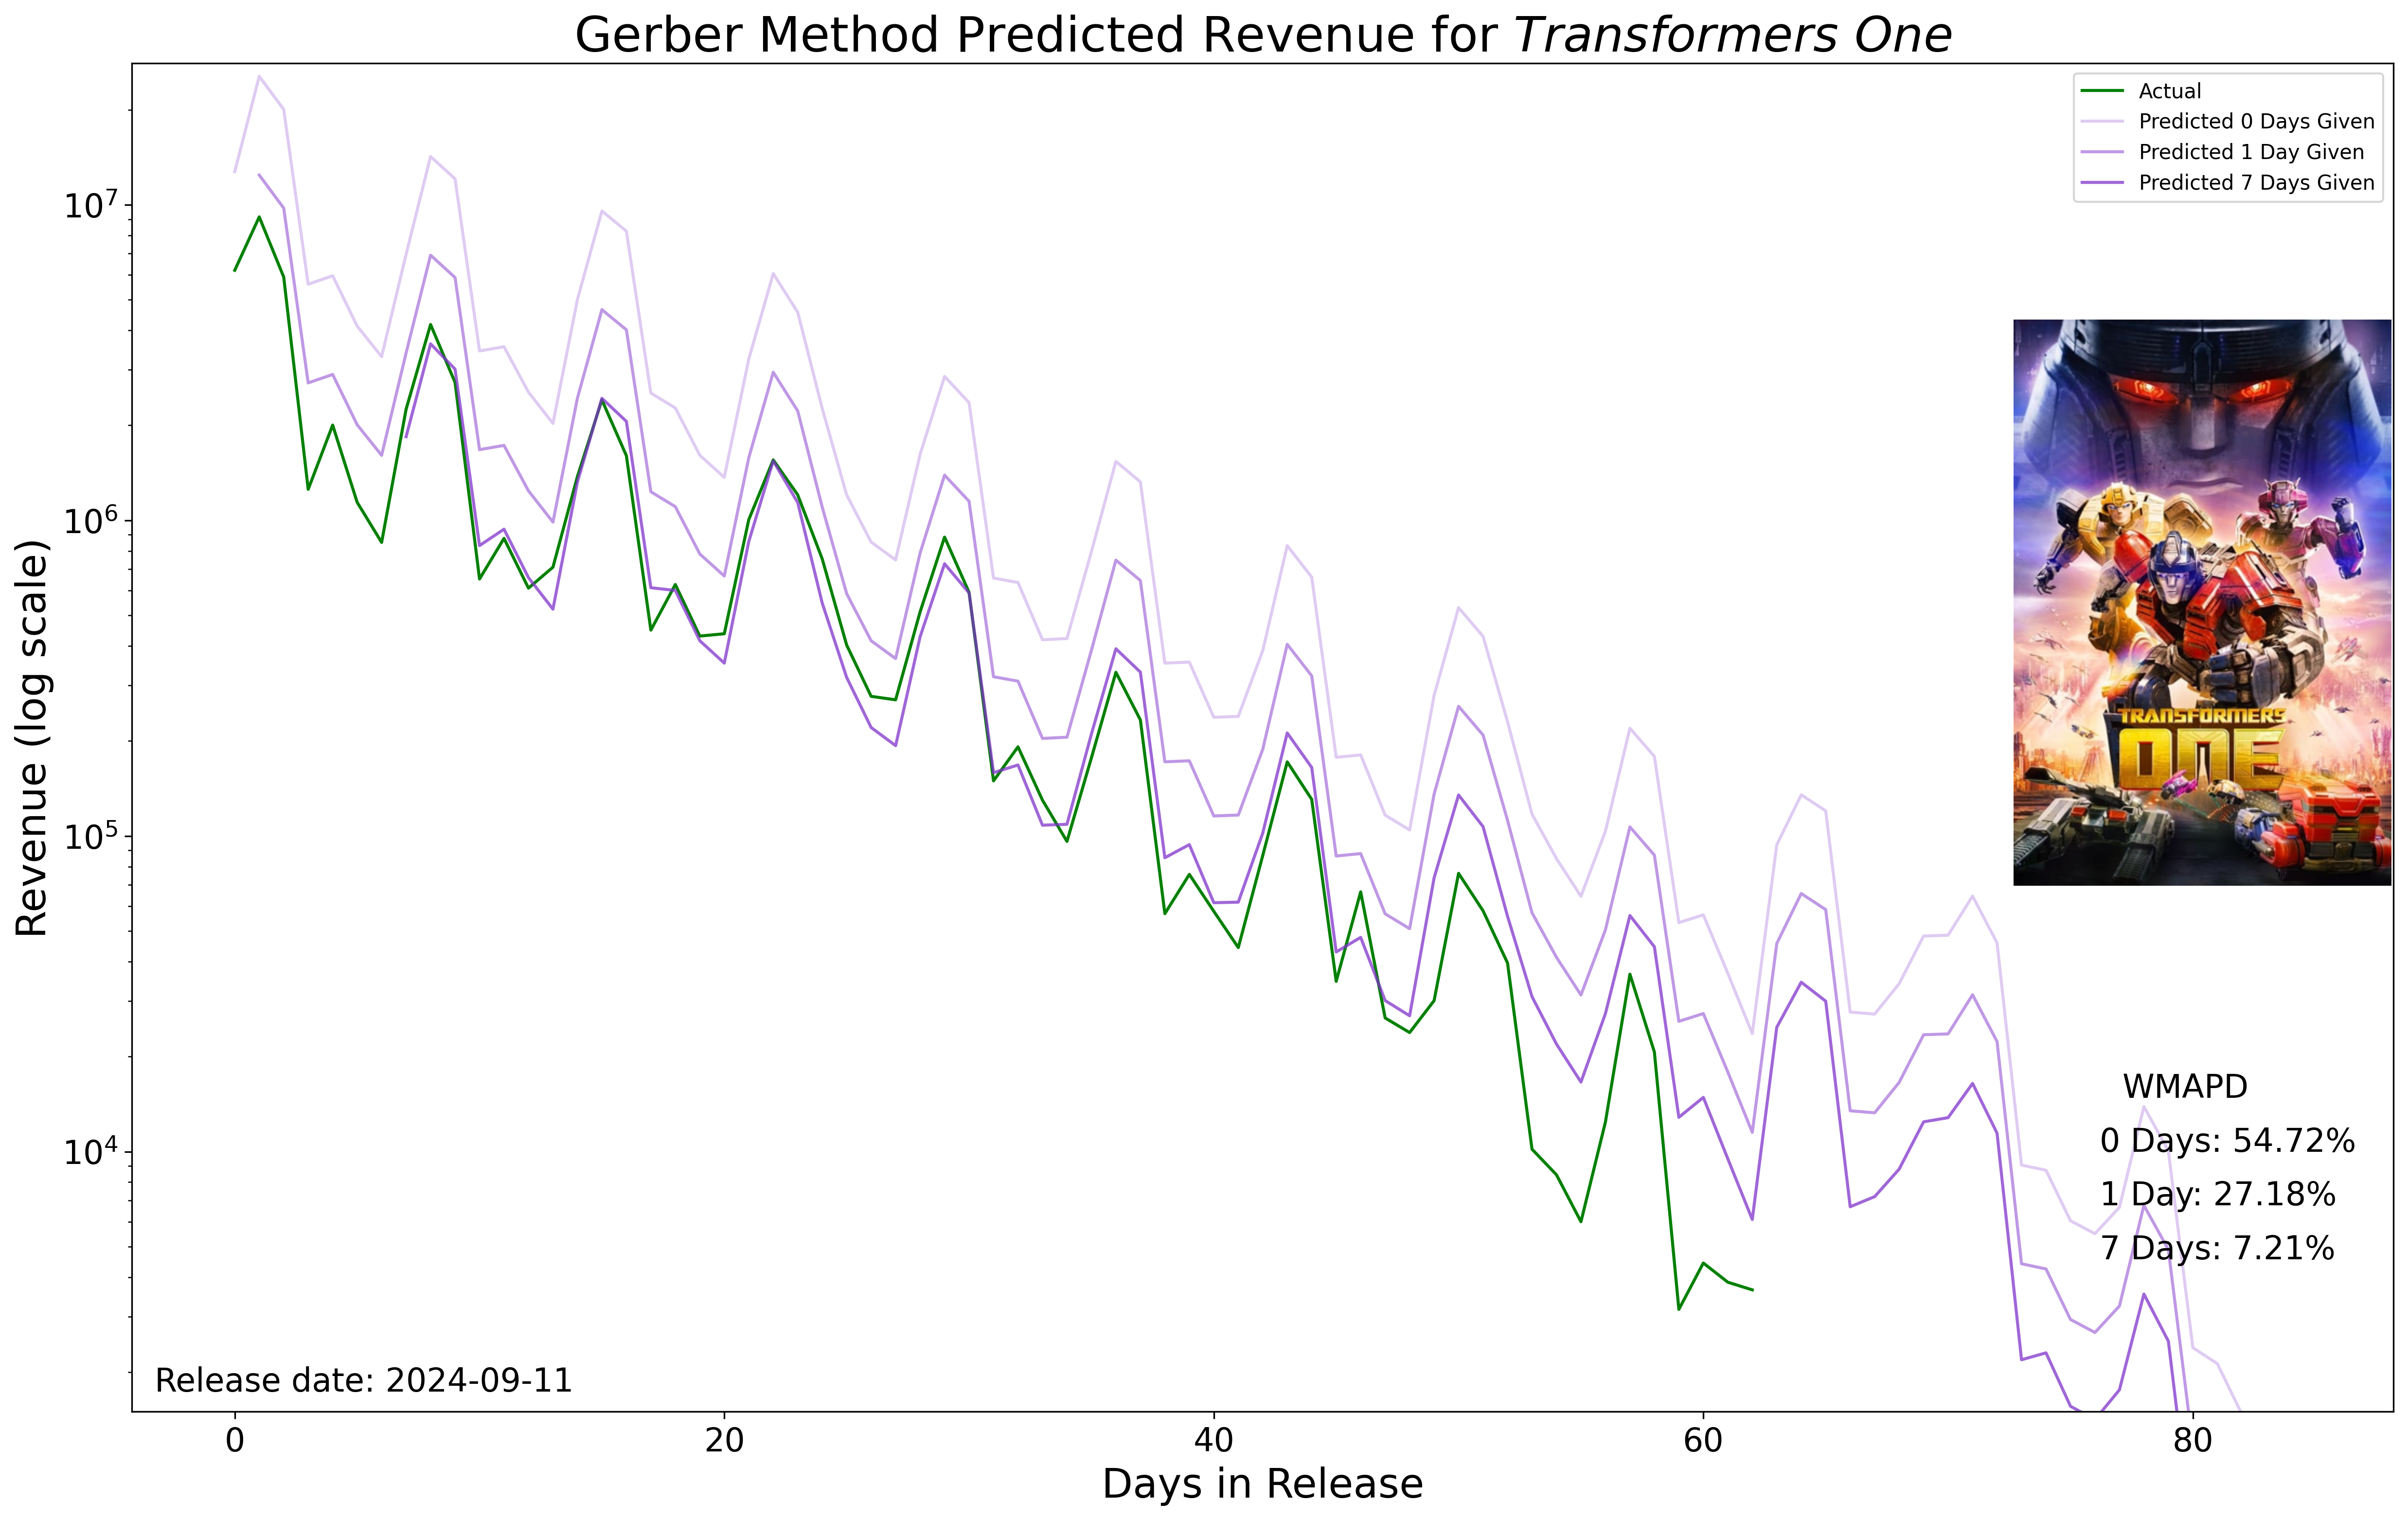
\includegraphics[width=0.95\textwidth]{../shared/images/pred/Transformers One_multiple_3.png}
  \end{figure}
  \addtocounter{framenumber}{-1}
\end{frame}

\begin{frame}{Results Multiple: \cite{transformersOne}}
  \begin{figure}
    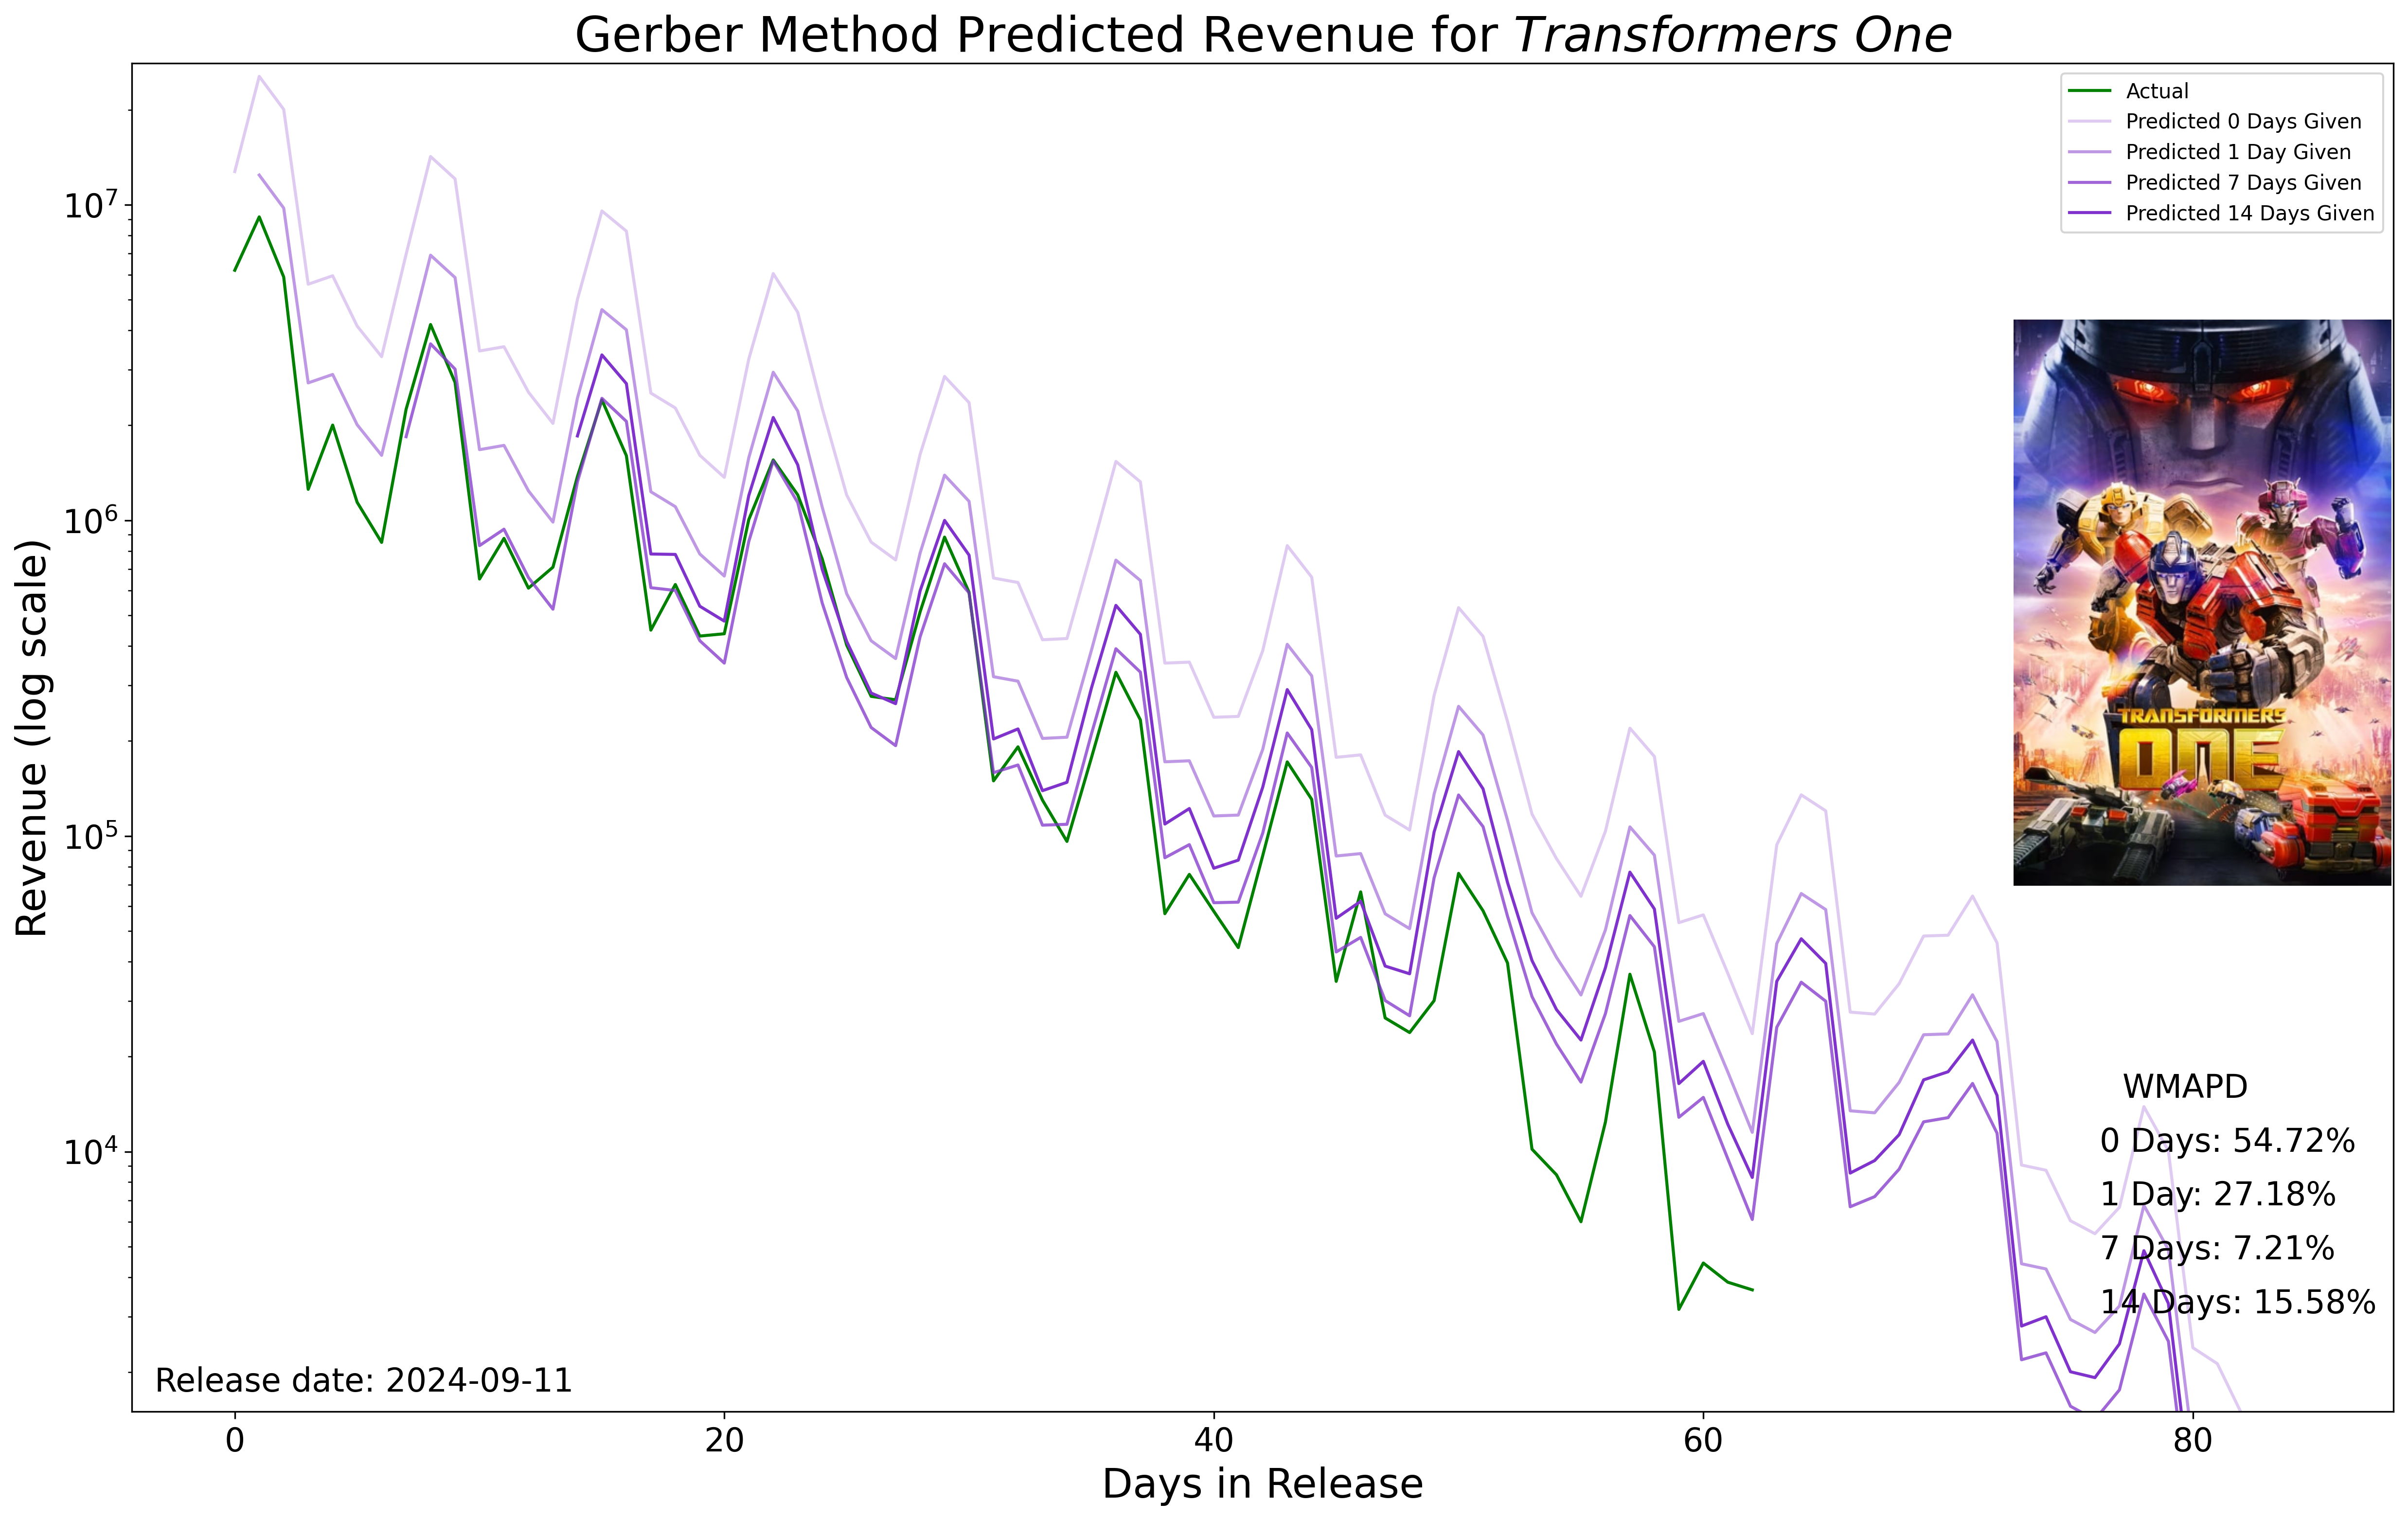
\includegraphics[width=0.95\textwidth]{../shared/images/pred/Transformers One_multiple_4.png}
  \end{figure}
  \addtocounter{framenumber}{-1}
\end{frame}

% alien romulus results multi
\begin{frame}{Results Multiple: \cite{alienRomulus}}
  \begin{figure}
    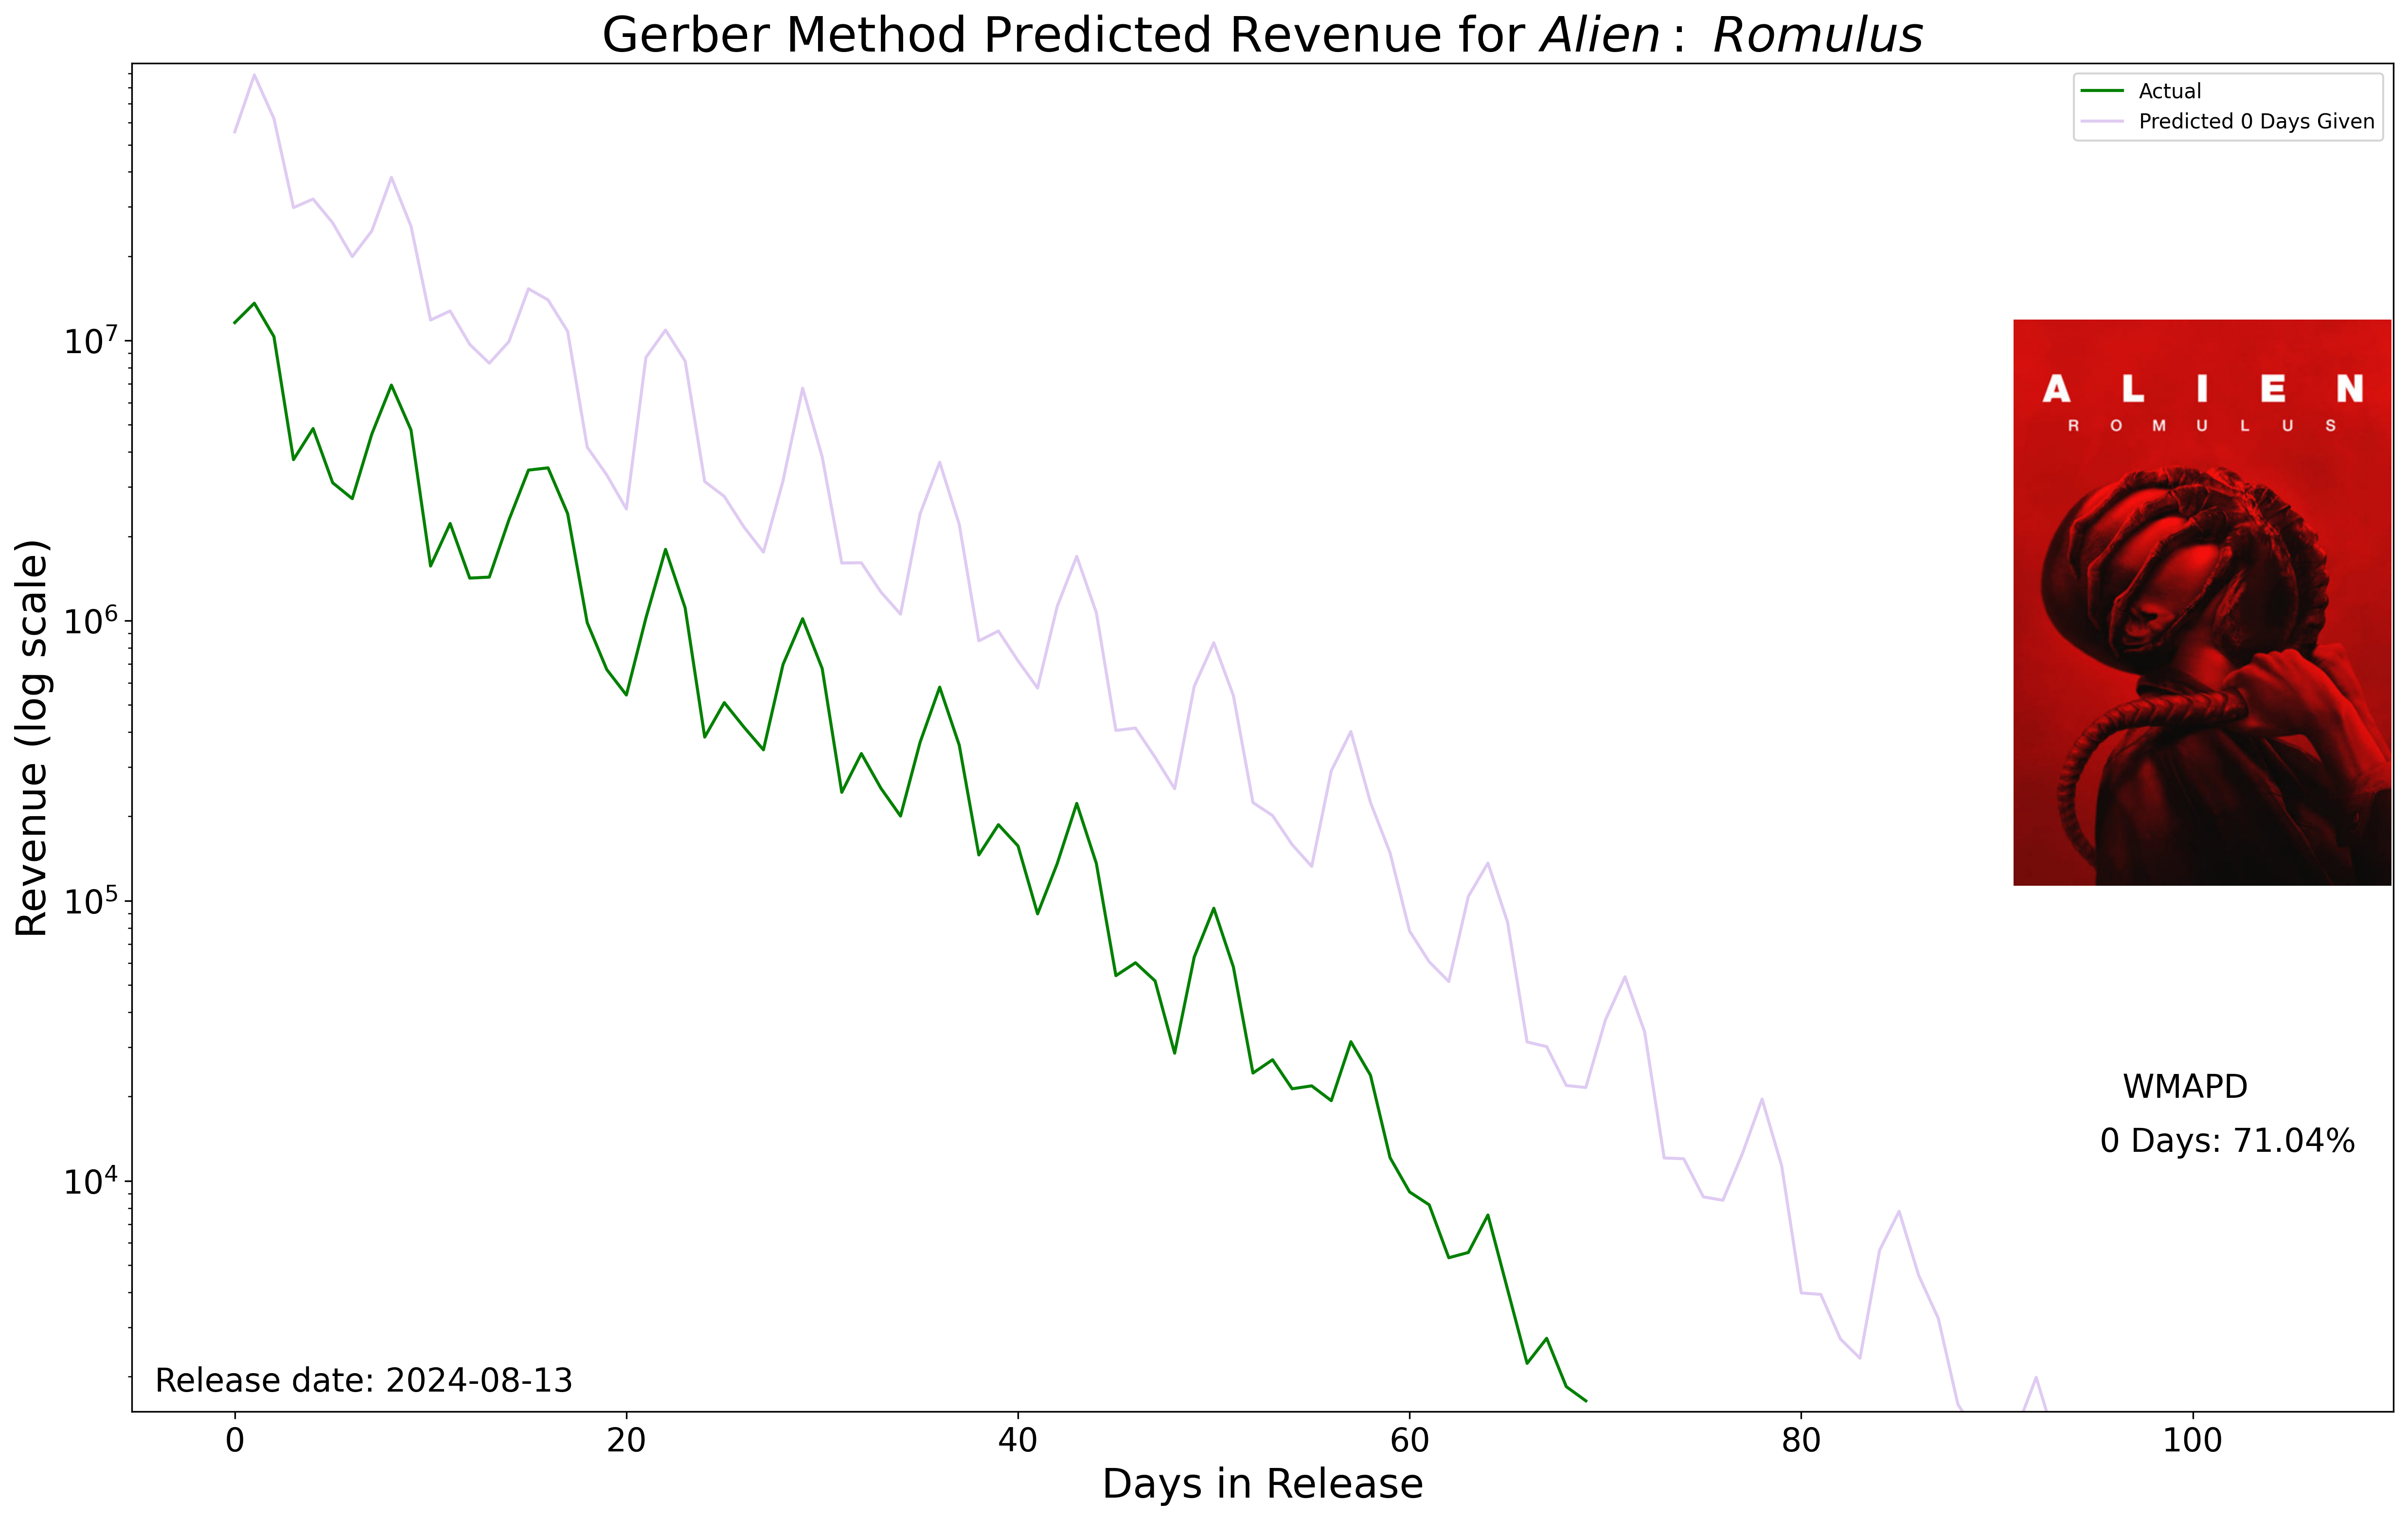
\includegraphics[width=0.95\textwidth]{../shared/images/pred/Alien: Romulus_multiple_1.png}
  \end{figure}
\end{frame}

\begin{frame}{Results Multiple: \cite{alienRomulus}}
  \begin{figure}
    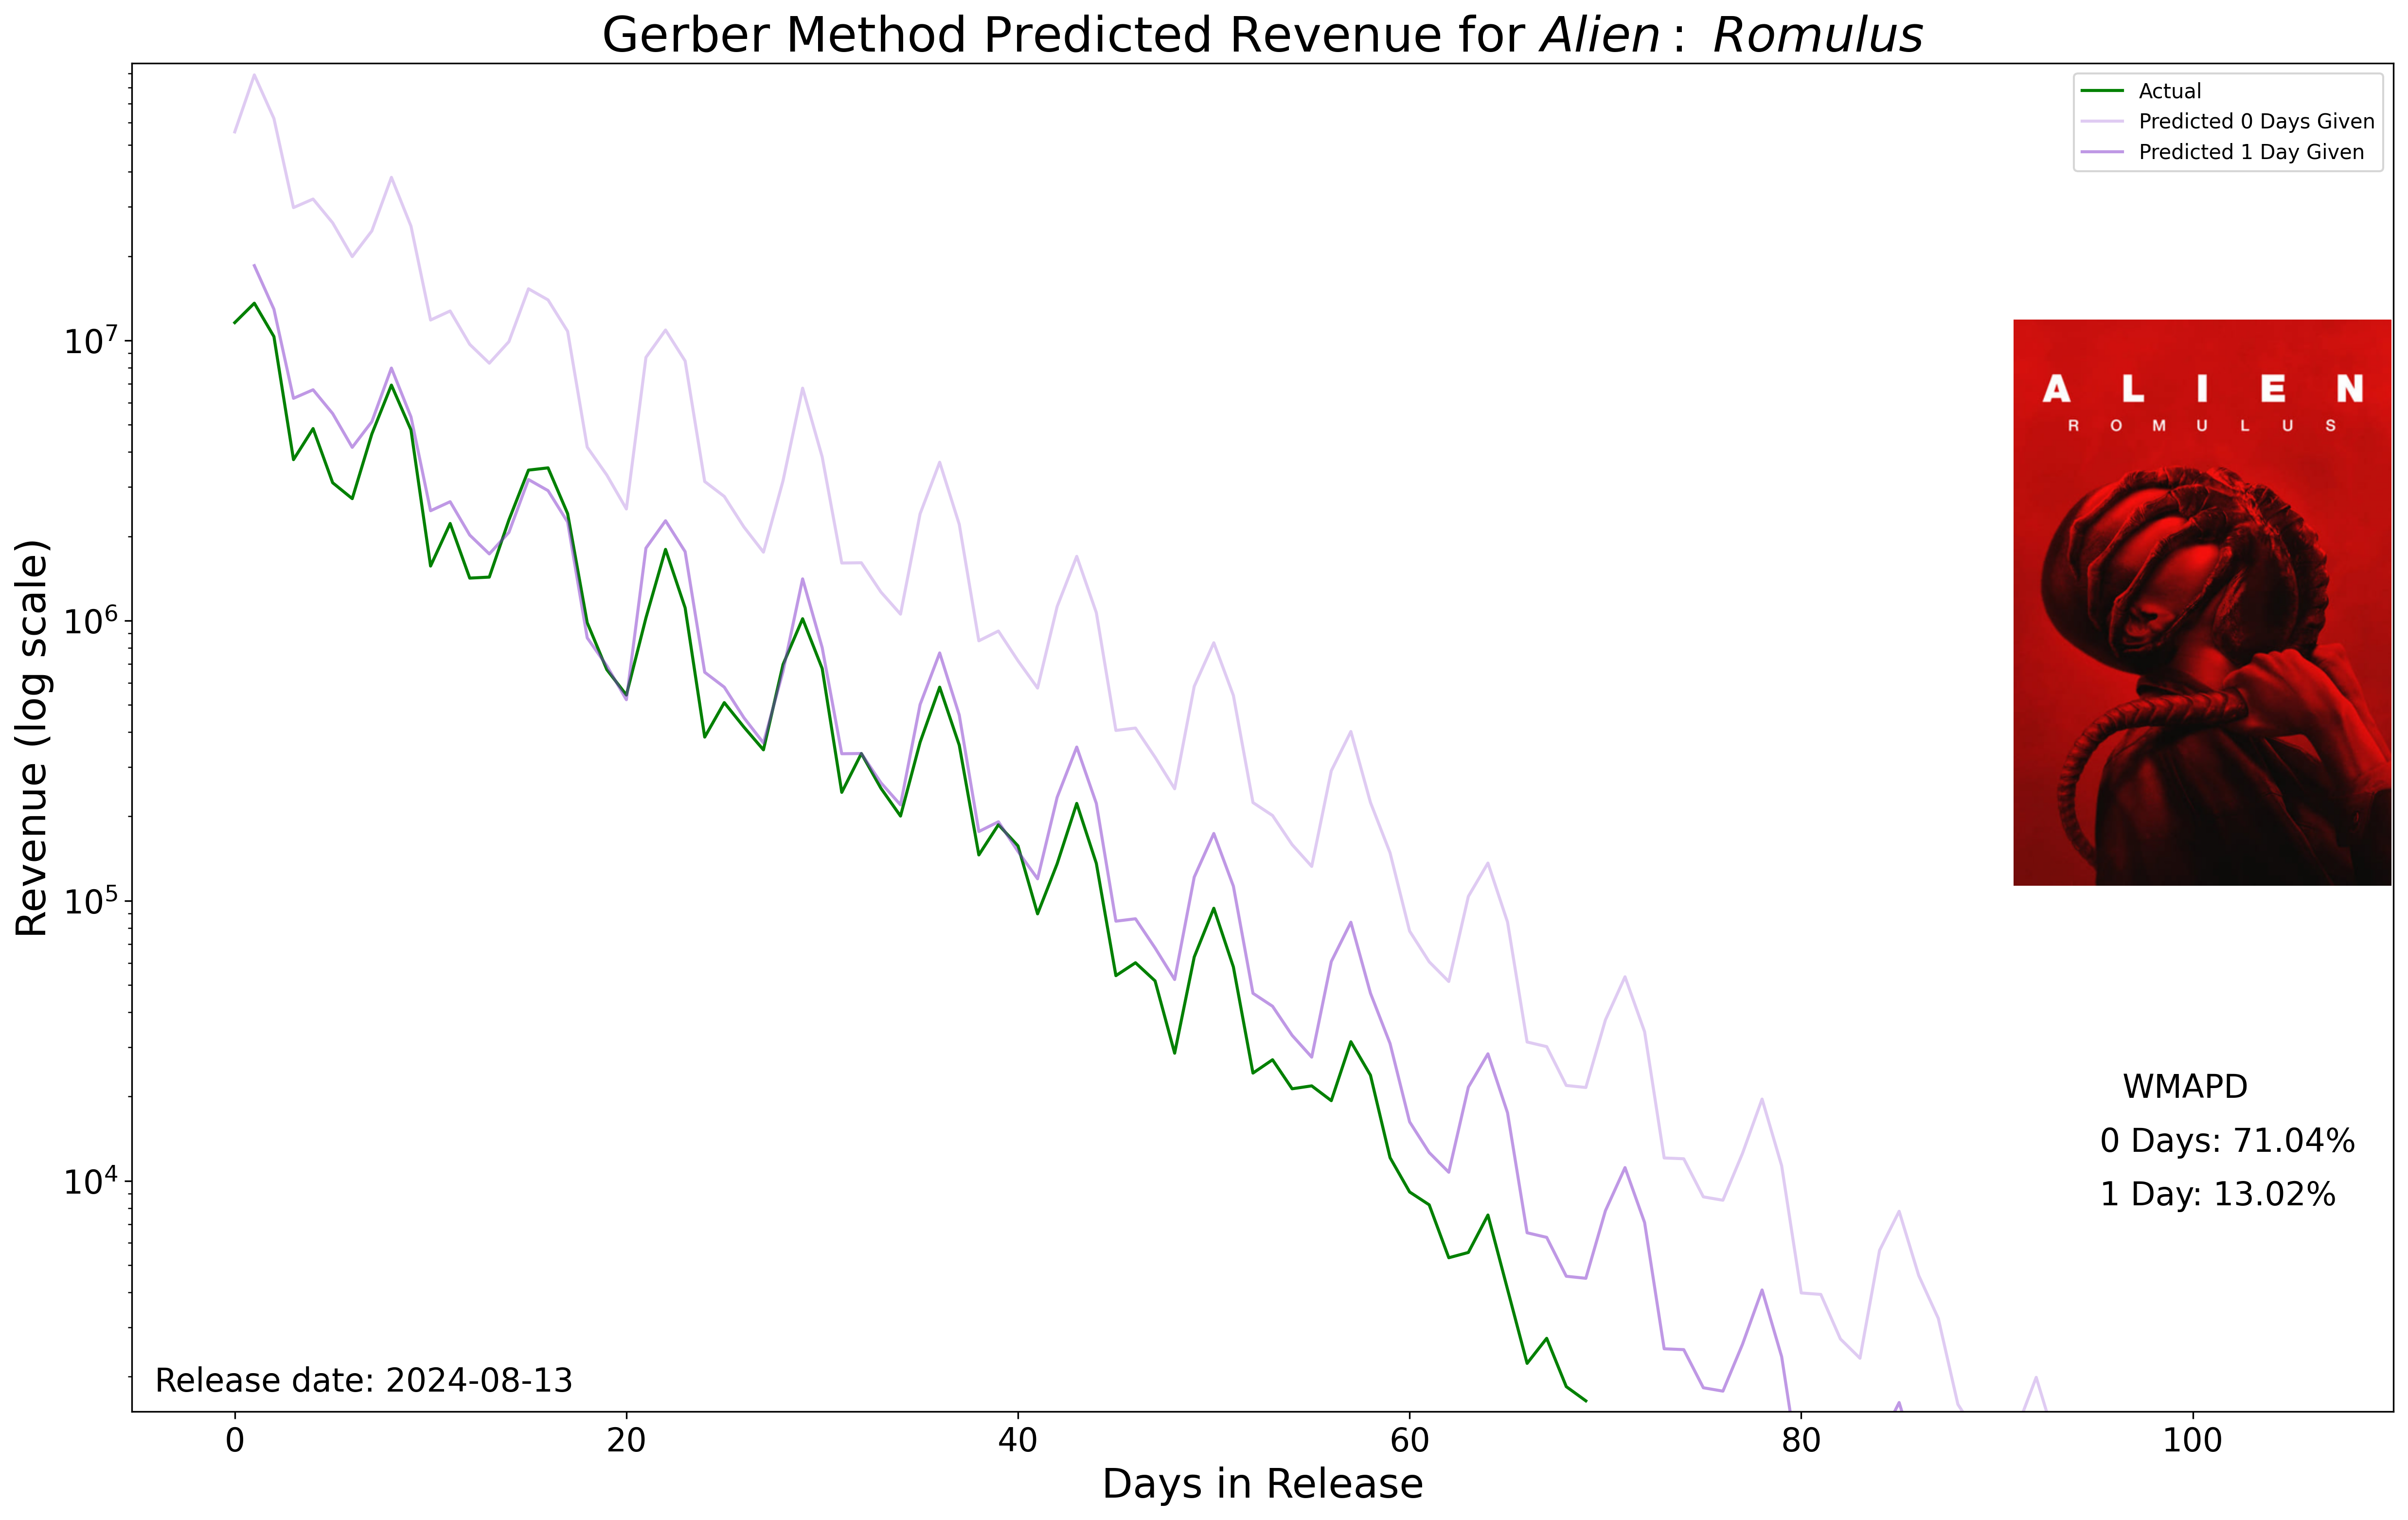
\includegraphics[width=0.95\textwidth]{../shared/images/pred/Alien: Romulus_multiple_2.png}
  \end{figure}
  \addtocounter{framenumber}{-1}
\end{frame}

\begin{frame}{Results Multiple: \cite{alienRomulus}}
  \begin{figure}
    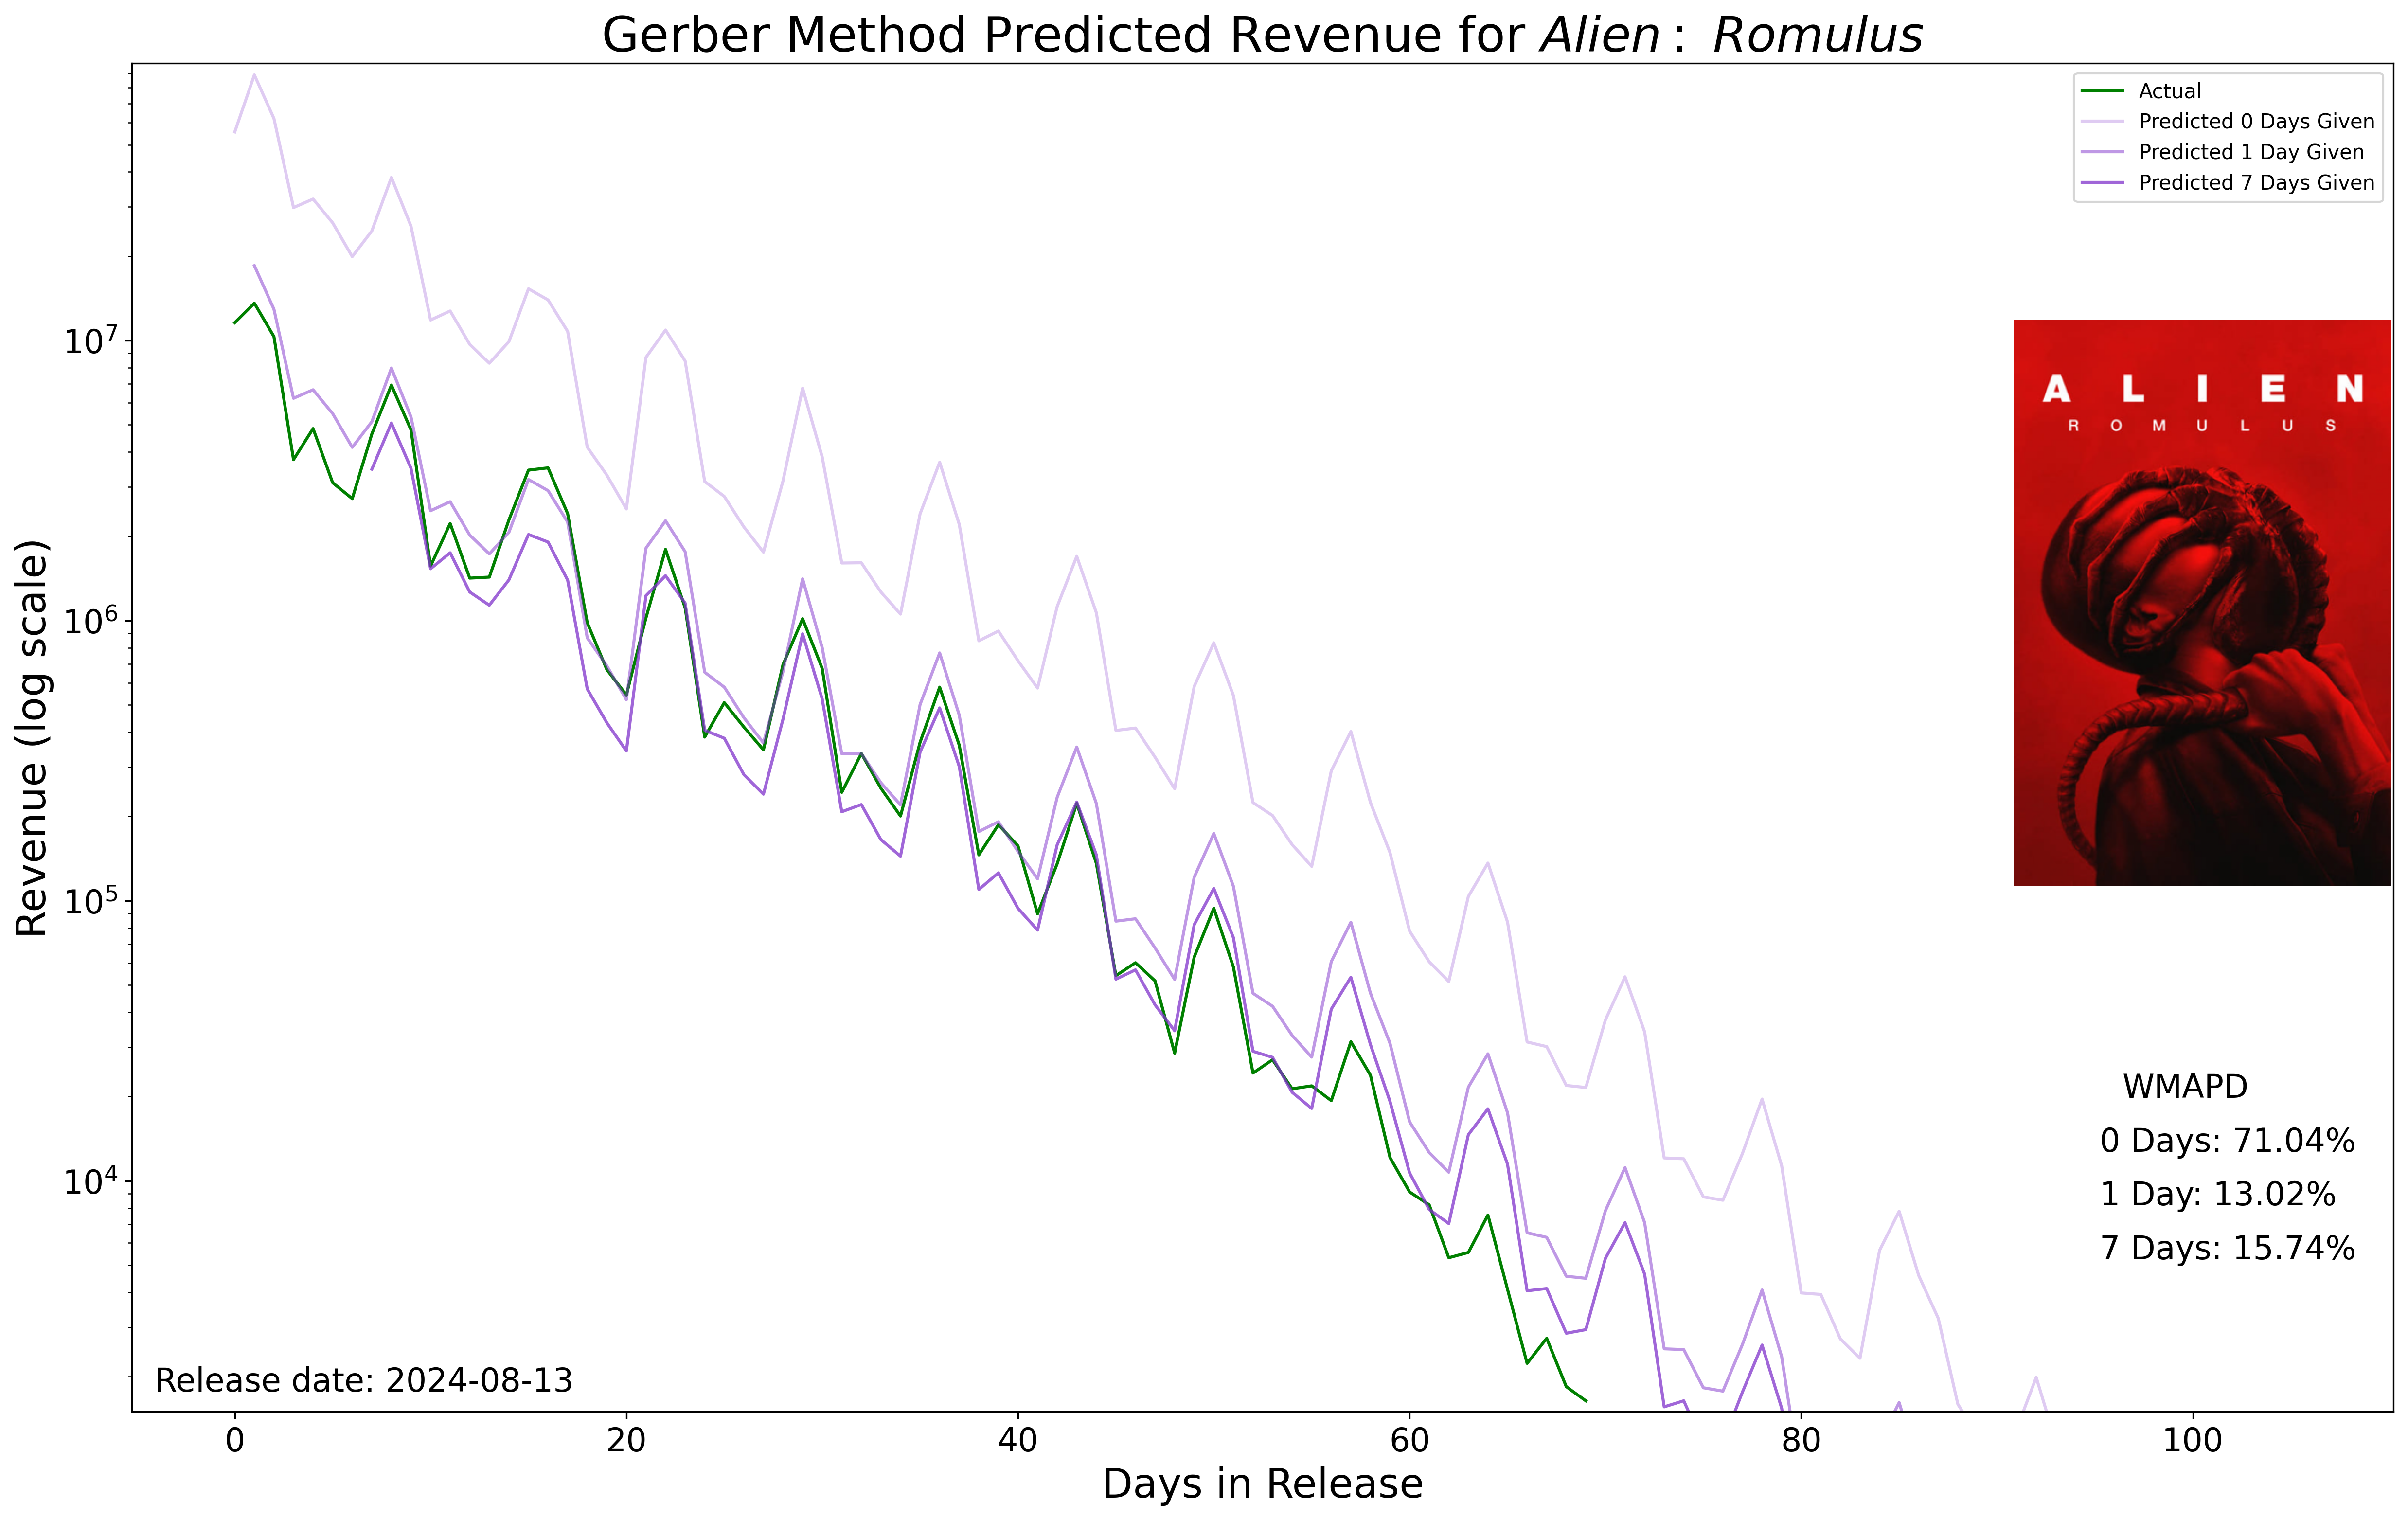
\includegraphics[width=0.95\textwidth]{../shared/images/pred/Alien: Romulus_multiple_3.png}
  \end{figure}
  \addtocounter{framenumber}{-1}
\end{frame}

\begin{frame}{Results Multiple: \cite{alienRomulus}}
  \begin{figure}
    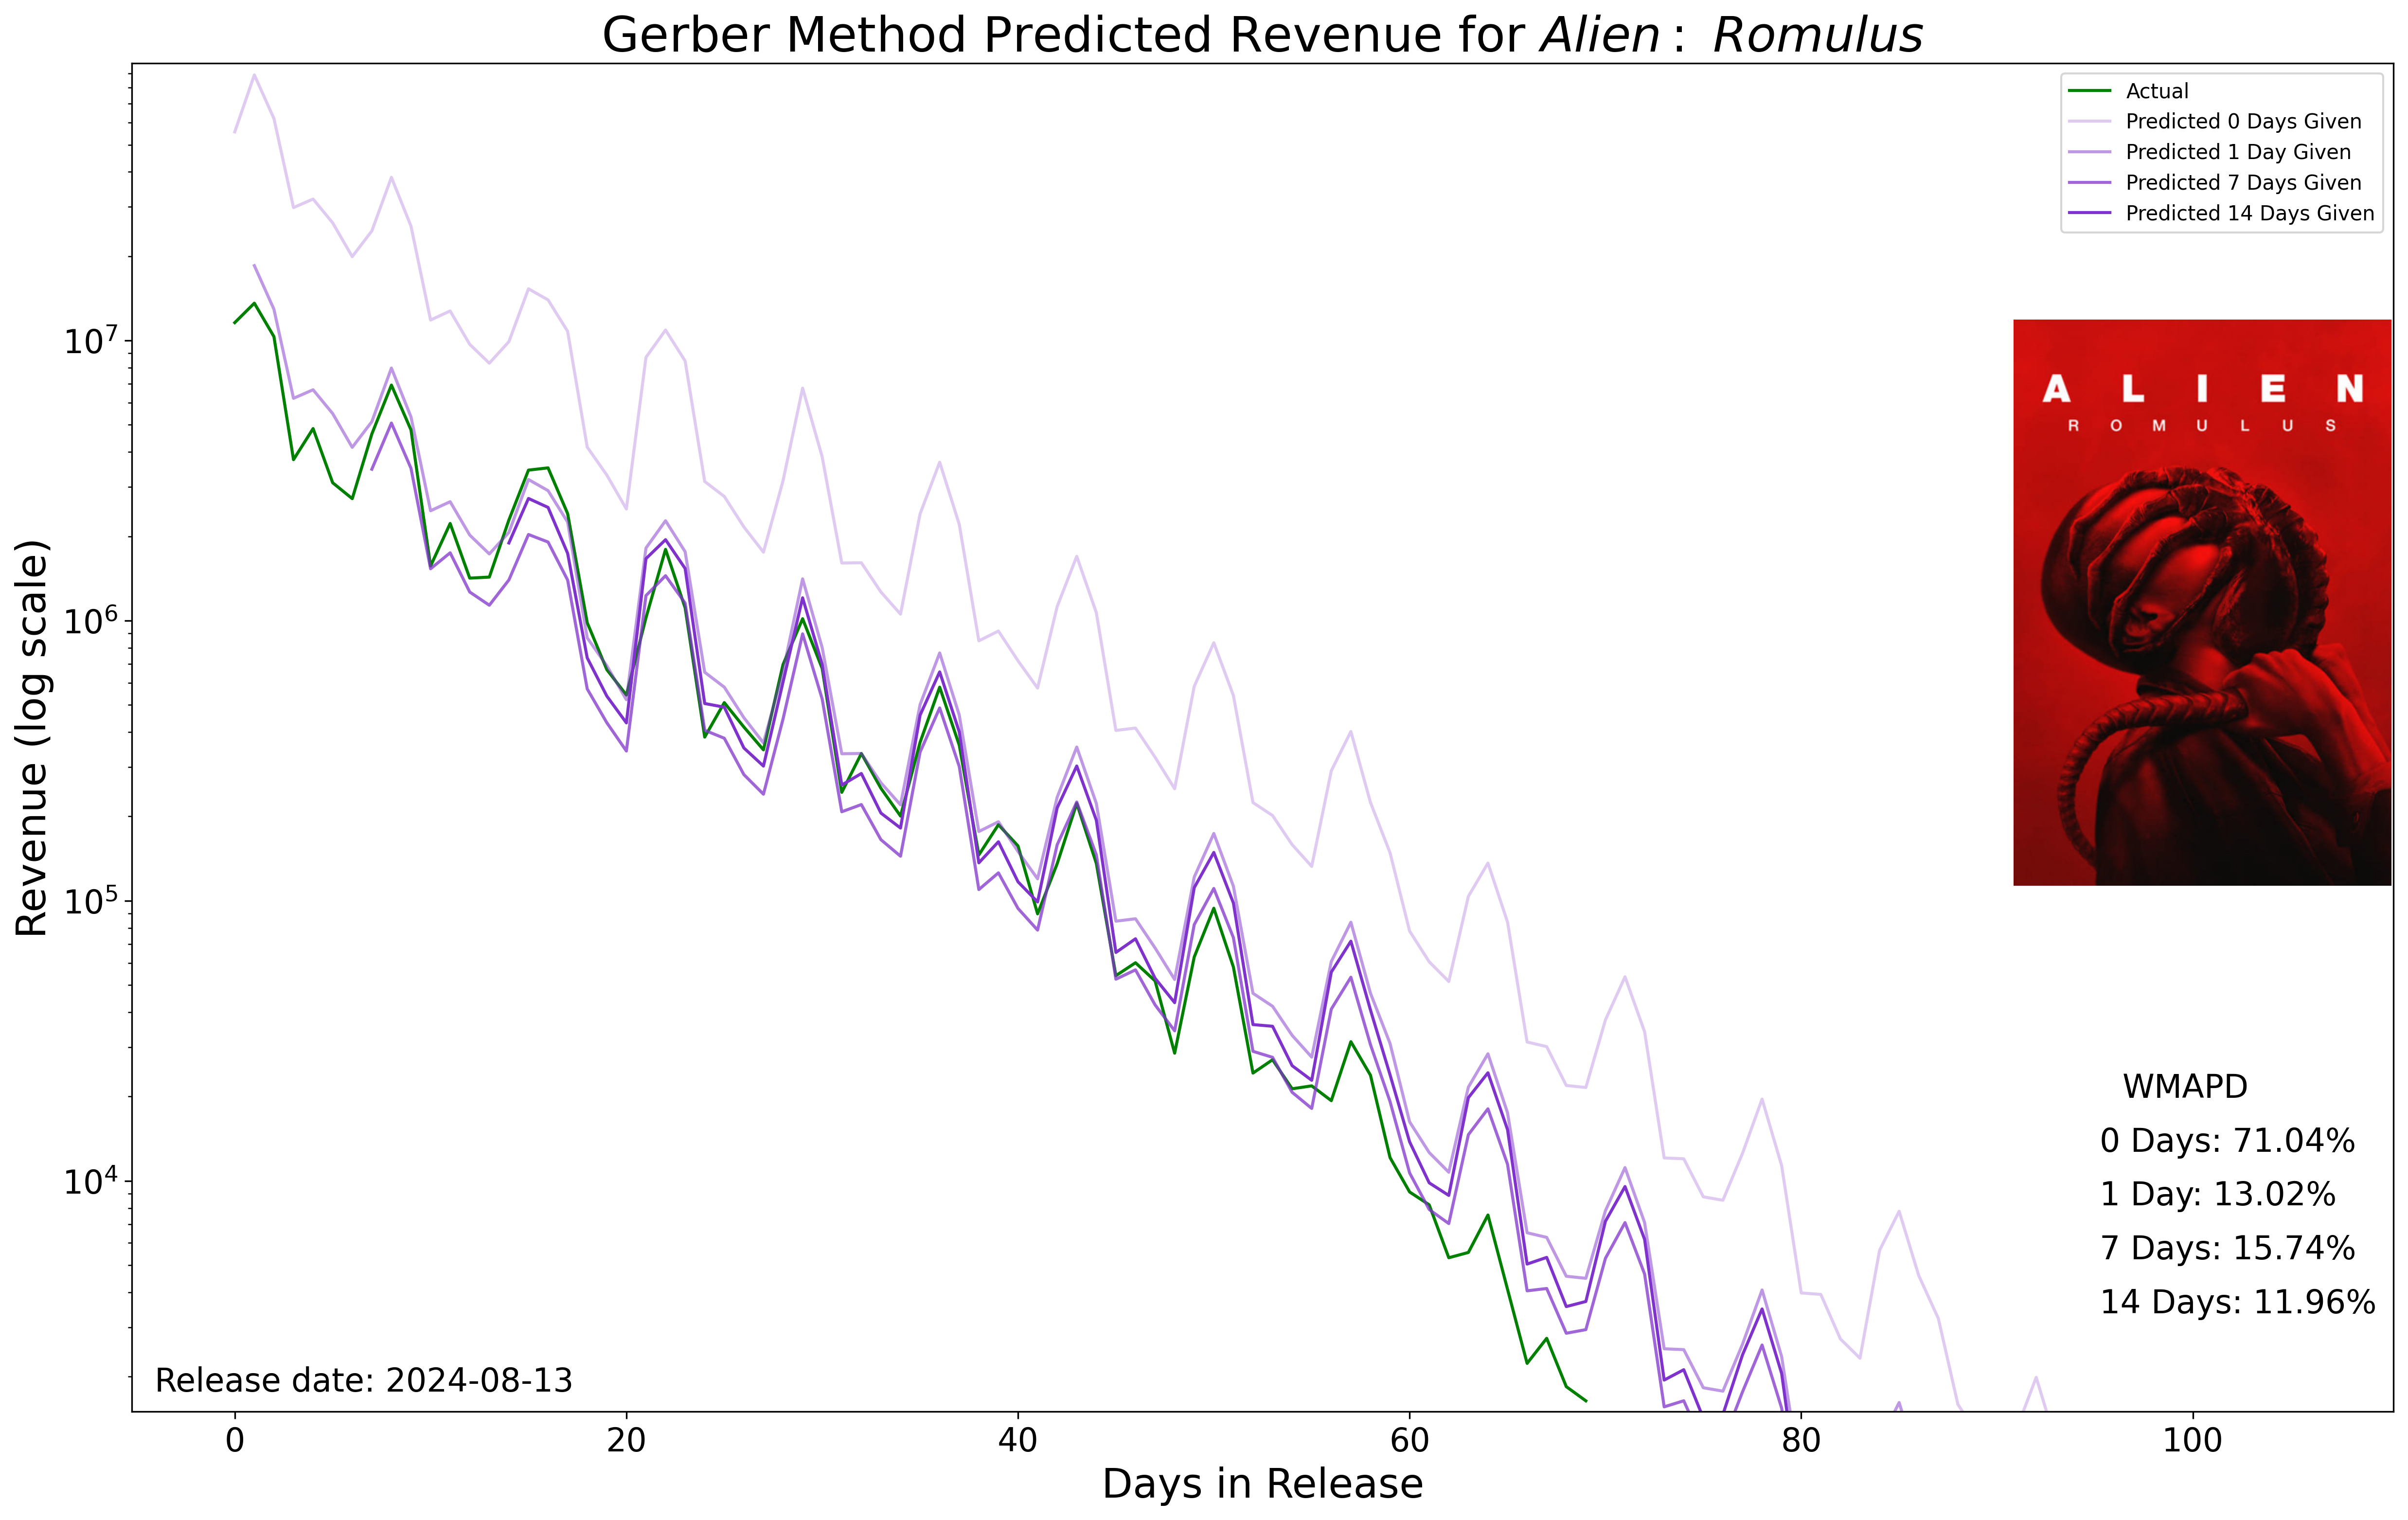
\includegraphics[width=0.95\textwidth]{../shared/images/pred/Alien: Romulus_multiple_4.png}
  \end{figure}
  \addtocounter{framenumber}{-1}
\end{frame}

\end{document}
